% !TEX encoding = UTF-8 Unicode
\documentclass[a4paper,twoside,italian,11pt]{book}
\usepackage{unibs-analisi2}

\hfuzz=3pt % To relax LaTeX about hbox overfullness

\hypersetup{
	pdftitle={Appunti di Analisi Matematica 2},
	pdfauthor={Federico Cerutti e Mauro Conte},
	pdfstartview={FitH},
	pdflang={it},
	pdfsubject={Appunti del corso di Analisi Matematica 2 del prof. Rinaldo M. Colombo},
	colorlinks = true,
	linkcolor = blue,
	anchorcolor = blue,
	citecolor = blue,
	filecolor = blue,
	urlcolor = blue
}

\begin{document}
\pagestyle{headings}

\frontmatter
\begin{titlepage}
	\begin{center}
		{\huge\bfseries Appunti di Analisi Matematica 2\\}
		% ----------------------------------------------------------------
		\vspace{1.5cm}
		{\Large\bfseries Federico Cerutti\\Mauro Conte\\}
		% ----------------------------------------------------------------
		\vspace{2cm}
		{Dal corso del professor}\\[5pt]
		\emph{{Rinaldo M. Colombo}}\\[2cm]
		\vfill
		% ----------------------------------------------------------------
		
\includegraphics[width=0.19\textwidth]{unibs-logo.png}\\[5pt]
		{Università degli Studi di Brescia}\\[10pt]
		{Ultimo aggiornamento: \today}
	\end{center}
\end{titlepage}

% Colophon
~
\vfill
\doclicenseThis

\cleardoublepage
\pdfbookmark[0]{\contentsname}{toc}
\tableofcontents


\mainmatter
\chapter*{Prefazione}\label{chap:foreword}
\addcontentsline{toc}{chapter}{Prefazione}
% The 2nd parameter of markboth may be left blank since this is a twoside document,
% but has been nonetheless specified to avoid future oversights.
\markboth{\MakeUppercase{Prefazione}}{\MakeUppercase{Prefazione}}
Questi appunti sono basati sulla dispensa \textit{Appunti per il Secondo Corso di Analisi Matematica per Allievi Ingegneri} del professor Rinaldo M. Colombo dell'Università degli Studi di Brescia. La stesura è stata resa necessaria dalla brevità delle dimostrazioni offerte nel testo ufficiale del corso, nonché dall'esigenza per gli autori di formalizzare i passaggi seguiti mentalmente durante lo studio.
\vspace*{\baselineskip}

\cbstart
Le parti di questo documento affiancate da una banda verde non sono state trattate a lezione e son riportate dal libro per completezza.
\cbend

\vfill
\noindent La versione più recente del testo è reperibile nel repository
\begin{center}
	\url{https://github.com/ceres-c/unibs-analisi2}
\end{center}
accessibile anche scansionando il seguente QRCode
\begin{center}
	
\includegraphics[width=.2\linewidth]{repository-qr}
\end{center}
Gli appunti non sono stati validati dal professore, dunque non si escludono errori. Son ben accette pull request per correggere inesattezze o migliorare spiegazioni.

\chapter{Spazi Metrici}

\section{Preliminari}
% TODO definzione campo

\begin{definition}[Spazio Vettoriale]
	Siano $K$ un \textbf{campo} e $V$ un \textbf{insieme}. Si dice che \textbf{Spazio Vettoriale} sul campo $K$ se sono definite due operazioni:
	\begin{enumerate}
		\item \textbf{Somma}, operazione interna binaria
		\item \textbf{Prodotto per scalari} operazione esterna
	\end{enumerate}
	\begin{note}
		Questa definizione è stata riportata per ricordare il concetto, si consiglia la consultazione di un libro di Algebra Lineare per una definizione più precisa.
	\end{note}
\end{definition}

\begin{definition}[Spazio Metrico]
	\label{def:sp_metrico}
	Si dice Spazio Metrico $(X,d)$ un insieme $X$ non vuoto in cui sia definita una \textbf{Distanza} (o \textbf{Metrica}), vale a dire una funzione $d: X \times X \to \R$ con le seguenti proprietà:
	\begin{enumerate}
		\item $d(x,y) \geq 0 \quad \forall x,y \in X$
		\item \label{itm:dist_0_iff_x_uguale_y} $d(x,y) = 0 \quad \forall x,y \in X \iff x=y$
		\item $d(x,y) = d(y,x) \quad \forall x,y \in X$ \quad(\textit{simmetria})
		\item $d(x,z) \leq d(x,y)+d(y,z) \quad \forall x,y,z\in X$ \quad(\textit{disuguaglianza triangolare})
	\end{enumerate}
	\begin{note}
		D'ora in poi, quando si userà $d$ come metrica, dove non diversamente specificato, si intenderà la \textbf{Metrica Euclidea} di \hyperref[ex:dist_eucl]{\cref*{ex:metriche} (\nameref*{ex:metriche})} % NOTE The \fullref command was not used on purpose to point this link straight to the right part of the aforementioned exercise
	\end{note}
\end{definition}

Unendo le due definizioni si giunge naturalmente a
\begin{definition}[Spazio Vettoriale Metrico]
	\label{def:sp_vett_normato}
	Uno \textbf{Spazio Vettoriale Metrico} è uno spazio vettoriale $V$ su cui è definito un prodotto scalare $<\cdot,\cdot·>$ definito positivo, la sua \textbf{Metrica}.
	\begin{note}
		Analogamente si definisce il Sottospazio Vettoriale Metrico
	\end{note}
\end{definition}

\begin{definition}[Metrica Indotta]
	\label{def:metr_indotta}
	Siano $(X,d)$ spazio metrico e $S \subseteq X$ con $S \neq \emptyset$\\
	Allora $d_{|S} = d_{|S \times S}$ è una metrica su $S$, cioè la metrica $d_{|S}$ è la \textbf{Metrica Indotta}, definita come la \textbf{restrizione} della metrica $d$ ai soli elementi di $S$. Si definisce formalmente come
	\[\funcdef{d_{|S}}{S \times S}{\R}{(x,y)}{d(x,y)}\]
\end{definition}

\begin{definition}[Sottospazio Metrico]
	Siano $(X,d)$ spazio metrico e $S \subseteq X$ con $S \neq \emptyset$\\
	Allora $(S,d_{|S})$ con la \fullref{def:metr_indotta} è a sua volta Spazio Metrico ed è chiamato \textbf{Sottospazio Metrico di $(X,d)$}
	\begin{proof}
		La $d_{|S}$, essendo restrizione della metrica $d$, rispetta ancora tutti i punti della \fullref{def:sp_metrico}.
	\end{proof}
\end{definition}

\begin{proposition}
	\label{prop:subspace_condition}
	Sia $(V)$ uno \textbf{spazio vettoriale metrico} sul campo $K$ e sia $\emptyset \neq U \subseteq V$. Il sottoinsieme $U$ è un \textbf{sottospazio vettoriale metrico} se, e soltanto se, sono verificate le seguenti condizioni:
	\begin{enumerate}
		\item $\forall \mathbf{u}, \mathbf{u'} \in U \quad \mathbf{u} + \mathbf{u'} \in U$
		\item $\forall \lambda \in K,\; \forall \mathbf{u} \in U \quad \lambda \cdot \mathbf{u} \in U$
	\end{enumerate}
	\begin{proof}
		Non richiesta, analoga a quella per Spazi Vettoriali reperibile in un libro di Algebra Lineare
	\end{proof}
\end{proposition}

\begin{example}[Esempi di Metriche]
	\label{ex:metriche}
	Si dimostri che le seguenti funzioni sono distanze:
	\begin{note}
		Si noti che alcuni degli esempi sottostanti sono relativi a metriche trattate molto più avanti e dunque potrebbe essere conveniente ignorarli temporaneamente per tornare qui quando saranno stati fatti i successivi argomenti.
	\end{note}
	\begin{enumerate}
		\item $X=\R^2,\quad d(x,y) = d\bigl((x_1,x_2),(y_1,y_2)\bigr) = \sqrt{(y_1-x_1)^2+(y_2-x_2)^2}$
			\hfill {
				\footnotesize\textbf{Metrica Euclidea in $\R^2$}
			}
			\begin{enumerate}[label=\arabic*]
				\item $d(x,y) \geq 0$ è verificata poiché l'argomento della radice è sempre positivo o al più nullo, essendo una somma di quadrati. Inoltre la radice quadrata mantiene la positività.
				\item $d(x,y) = 0 \iff x = y$
					\begin{align*}
						d = 0 &\iff \sqrt{(y_1-x_1)^2+(y_2-x_2)^2} = 0\\
						&\iff (y_1-x_1)^2+(y_2-x_2)^2 = 0\\
						&\iff \begin{cases}
							(y_1-x_1)^2=0\\
							(y_2-x_2)^2=0\\
						\end{cases}\\
						&\iff
						\begin{cases}
							y_1=x_1\\
							y_2=x_2\\
						\end{cases}\\
						&\iff (x_1,x_2)=(y_1,y_2)
					\end{align*}
				\item $d(x,y) = d(y,x)$ invertendo le coordinate di $x$ con quelle di $y$ la somma non cambia, quindi la simmetria è rispettata
					\begin{align*}
						d\bigl((x_1,x_2),(y_1,y_2)\bigr) \bigr)
						&= \sqrt{(y_1-x_1)^2+(y_2-x_2)^2}\\
						&= \sqrt{(y_2-x_2)^2+(y_1-x_1)^2}\\
						&= d\bigl((y_1,y_2),(x_1,x_2)\bigr)
					\end{align*}
				\item $d(x,y) \leq d(x,z) + d(z,y)$ da \fullref{prop:dist_sp_norm}, la metrica indotta dalla norma (\fullref{def:norma}), applicata ad $\R^2$ è
					\[\norm{x - y} = \sqrt{(y_1-x_1)^2+(y_2-x_2)^2}\]
					che corrisponde alla metrica in oggetto. Dunque, grazie alle proprietà dell'operatore $\norm{\;\cdot\;}$ (nello specifico la \textit{disuguaglianza triangolare}), si ottiene
					\[d(x,y) = \norm{x-y} = \norm{(x-z) + (z-y)} \leq \norm{x-z} + \norm{z-y} = d(x,z) + d(z,y)\]
					\begin{center}
						\begin{tikzpicture}[scale=0.5]
						\draw (0,0) node[anchor=north east]{$x=(x_1,x_2)$}
							-- (4,4) node[anchor=south]{$y=(y_1,y_2)$}
							-- (4,0) node[anchor=north west]{$z=(z_1,z_2)$}
							-- cycle;
						\end{tikzpicture}
					\end{center}
			\end{enumerate}
		\item $X=\R,\quad d(x,y)=\abs{y-x}$
			\hfill {\footnotesize\textbf{Metrica Euclidea in} $\R$}
			\begin{enumerate}[label=\arabic*.]
				\item $d(x,y) \geq 0$ per definizione di valore assoluto
				\item $d(x,y) = 0 \iff x = y$ perché $\abs{\;\cdot\;} = 0 \iff \cdot\; = 0$, per definizione di valore assoluto
				\item $d(x,y)=d(y,x)$ perché $\abs{x - y} = \abs{y - x}$ per definizione di valore assoluto
				\item $d(x,y) \leq d(x,z) + d(z,y)$ in quanto
					\[d(x,y) = \abs{x-y} = \abs{x-z+z-y} \leq \abs{x-z} + \abs{z-y} = d(x,z) + d(z,y)\]
			\end{enumerate}
		\item \label{ex:dist_eucl}
			$\begin{array}{l}
				X=\R^n \text{ con } x=(x_1,\ldots,x_n),\; y=(y_1,\ldots,y_n)\\
				d(x,y)=\sqrt{\sum\limits_{i=1}^{n}{\left(y_i-x_i\right)}^2}
			\end{array}$
			\hfill
			{
				\footnotesize\textbf{Metrica Euclidea in} $\R^n$
			}\\
			Analogo al primo esempio.
		\item \label{ex:dist_discr}
			$
				X\ne \emptyset,\quad d(x,y)=
				\begin{cases}
					\begin{array}{ll}
						0 & x = y\\
						1 &x \ne y
					\end{array}
				\end{cases}
			$
			\hfill {\footnotesize\textbf{Metrica Discreta}}
			\begin{enumerate}[label=\arabic*.]
				\item $d(x,y) \geq 0$ per definizione della metrica
				\item $d(x,y) = 0 \iff x = y$ per definizione della metrica
				\item $d(x,y)=d(y,x)$ per definizione della metrica (sia nel caso $x = y$ che in $x \neq y$)
				\item $d(x,y) \leq d(x,z) + d(z,y)$ perché $d(x,z) + d(z,y)$ può essere:
					\begin{itemize}
						\item $0$ se $x = y = z$, ma in questo caso anche $d(x,y) = 0$
						\item $1$ se $x = y \neq z$ o $x \neq y = z$, ma in questo caso $d(x,y) \leq 1$
						\item $2$ se $x \neq y \neq z$, quindi sicuramente $d(x,y) \leq d(x,z) + d(z,y)$
					\end{itemize}
			\end{enumerate}
		\item \label{ex:dim_dist_conv_unif}
			$
				\begin{array}{l}
					X = \cntclass{0}(\intervalclose{a}{b};\R)\; a,b \in \R,\; a < b\\
					d_\infty(f,g) = \sup\limits_{x \in \intervalclose{a}{b}} \abs{g(x) - f(x)}
				\end{array}
			$
			\hfill
			{
				\footnotesize
				\begin{tabular}{c}
					\textbf{Distanza della Convergenza Infinita}\\[-1ex]
					o\\[-1ex]
					\textbf{Distanza della Convergenza Uniforme}
				\end{tabular}
			}
			\begin{note}
				La metrica viene trattata in \fullref{def:conv_unif}
			\end{note}
			\begin{note}
				$X$ è l'insieme delle infinite funzioni continue nell'intervallo $\intervalclose{a}{b}$.
			\end{note}
			\begin{center}
				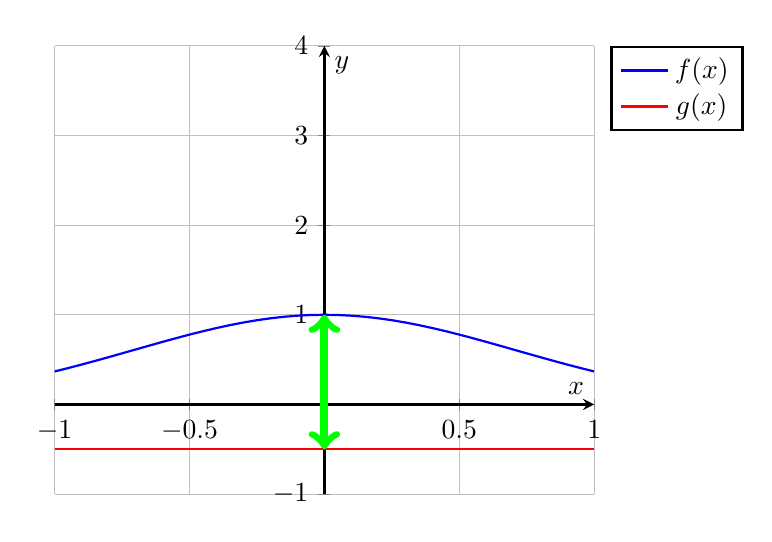
\begin{tikzpicture}[scale=1]
					\begin{axis}[
						xlabel={$x$},ylabel={$y$},
						axis lines=middle,
						samples=41,grid,thick,
						domain=-1:1,
						ymin=-1,ymax=4,
						legend pos=outer north east ]
						\addplot+[no marks] {e^-(abs(x*x))}; \addlegendentry{$f(x)$}
						\addplot+[no marks] {-0.5}; \addlegendentry{$g(x)$}
						\draw[<->,line width=1mm, color=green] (axis cs:0,-0.5) -- (axis cs:0,1);
					\end{axis}
				\end{tikzpicture}
			\end{center}
			\begin{enumerate}[label=\arabic*.]
				\item \label{itm:dist_conv_unif_geq_0} $d(x,y) \geq 0$ per definizione, il valore è sicuramente appartenente a $\intervalclose{0}{+\infty}$, ma $+\infty$ non è un valore accettabile, in quanto la metrica è definita come funzione a valori in $\R$ e $+\infty \notin \R$. D'alto canto, si nota che $X$ è definito come l'insieme delle funzioni continue definite su un intervallo \textbf{chiuso e limitato} a valori in $\R$ ($\cntclass{0}(\intervalclose{a}{b},\R)$). Questa definizione permette di applicare il \fullref{ex:weier_analisi_1} ed avere la certezza che esista $\sup$ finito.
				\item $d(x,y) = 0 \iff x = y$ per definizione, $d_\infty(f,g) = 0 \iff \sup\limits_{x\in\intervalclose{a}{b}}\abs{g(x)-f(x)} = 0$, cioè se e solo se le due funzioni hanno lo stesso dominio e, per ogni punto di esso, la stessa immagine.
				\item $d(x,y)=d(y,x)$ semplicmente $d_{\infty}(f,g) = \sup\limits_{x\in\intervalclose{a}{b}}\abs{f-g} = \sup\limits_{x\in\intervalclose{a}{b}}\abs{g-f} = d_{\infty}(g,f)$
				\item $d(x,y) \leq d(x,z) + d(z,y)$ dalla disuguaglianza triangolare per $\abs{\;\cdot\;}$ si ottiene
					\[\abs{g(x)-f(x)} \leq \abs{g(x)-h(x)}+\abs{h(x)-f(x)}\]
					Applicando il sup la disuguaglianza resta vera.
			\end{enumerate}
			\begin{note}
				Si sottolinea che queste conclusioni sono valide finché $\intervalclose{a}{b}$ chiuso e limitato, altrimenti non varrebbe più l'\fullref{ex:weier_analisi_1} che è necessario per il punto \ref{itm:dist_conv_unif_geq_0}. % TODO Serve un controesempio
			\end{note}
		\item \label{ex:dist_parigi}
			$
				\begin{array}{l}
					X=\R^2,\; d \text{ Metrica Euclidea e } P \in X \text{ punto arbitrario }\\
					d_P(x,y)=
					\begin{cases}
						\begin{array}{ll}
							0 & \text{se } x = y\\
							d(x,P) + d(P,y) & \text{se } x \neq y
						\end{array}
					\end{cases}
				\end{array}
			$
			\hfill
			{
				\footnotesize
				\begin{tabular}{c}
					\textbf{Distanza di Parigi}\\[-1ex]
					o\\[-1ex]
					\textbf{Distanza Ferroviaria Francese}
				\end{tabular}
			}
			\begin{enumerate}[label=\arabic*.]
				\item $d(x,y) \geq 0$ per definizione della metrica
				\item $d(x,y) = 0 \iff x = y$ per definizione della metrica
				\item $d(x,y)=d(y,x)$ essendo bassata sulla Metrica Euclidea
				\item $d(x,y) \leq d(x,z) + d(z,y)$ essendo bassata sulla Metrica Euclidea
			\end{enumerate}
		\item \label{ex:dim_dist_quadratica}
			$
				\begin{array}{l}
					X=\cntclass{0}(\intervalclose{a}{b},\R)\;a,b\in\R,\;a<b\\
					d_2(f,g) = \sqrt{\int_a^b\left[g(x)-f(x)\right]^2 \integrald{x}}
				\end{array}
			$
			\hfill
			{
				\footnotesize\textbf{Distanza Quadratica}
			}
			\begin{note}
				La metrica viene trattata in \fullref{def:dist_quadratica}
			\end{note}
			\begin{enumerate}[label=\arabic*.]
				\item $d(x,y) \geq 0$ per definizione, essendo integrale di un valore positivo (quadrato) tra estremi ordinati ($a<b$ per ipotesi)
				\item $d(x,y) = 0 \iff x = y$ Per definizione della metrica:
				\[d_2(f,g) = 0 \iff \sqrt{\int_a^b\left[g(x)-f(x)\right]^2 \integrald{x}} = 0\]
				cioè se e solo se le due funzioni hanno lo stesso dominio e, per ogni punto di esso, la stessa immagine.
				\item $d(x,y)=d(y,x)$ semplicmente $d_2(f,g) = \sqrt{\int_a^b\left[g(x)-f(x)\right]^2 \integrald{x}} = \sqrt{\int_a^b\left[f(x)-g(x)\right]^2 \integrald{x}} = d_2(g,f)$
				\item $d(x,y) \leq d(x,z) + d(z,y)$ ... % TODO Spiegare questo punto
			\end{enumerate}
	\end{enumerate}
\end{example}

\begin{definition}[Norma]
	\label{def:norma}
	Dato uno spazio vettoriale $V$ sul campo $\mathbb{K}$, si definisce \textbf{Norma} una funzione $\norm{\cdot}:V \to \R$ con le proprietà:
	\begin{enumerate}
		\item $\norm{x} \geq 0 \quad \forall x\in V$
		\item $\norm{x}=0 \iff x = 0 \quad \forall x\in V$
		\item \label{itm:def_norm_propr_somma} $\norm{x+y} \leq \norm{x}+\norm{y} \quad \forall x,y\in V$
		\item \label{itm:def_norm_propr_lambda} $\norm{\lambda x} = \abs{\lambda} \cdot \norm{x} \quad \forall x\in V,\lambda\in\mathbb{K}$
	\end{enumerate}
	\begin{note}
		La funzione Norma associa dunque ad un vettore di qualsiasi dimensione uno scalare, fornendo (anche) una metrica per ordinare vettori tra loro.
	\end{note}
\end{definition}
\begin{definition}[Spazio Normato]
	Uno \textbf{Spazio Normato} è uno spazio vettoriale $V$ sul campo $\mathbb{K}$ \textbf{in cui è definita una norma}.
	\begin{note}
		Nel seguito verranno considerati esclusivamente spazi vettoriali su $\R$ o su $\C$, cioè $\mathbb{K} = \R$ o $\mathbb{K} = \C$
	\end{note}
\end{definition}

\begin{example}[Esempi di Spazi Normati]\leavevmode\vspace*{-\baselineskip}
	\label{ex:sp_norm}
	\begin{enumerate}
		\item $\R$ con $\norm{x} = \abs{x}$
		\item $\C$ con $\norm{x} = \abs{x}$
		\item \label{itm:ex_sp_norm_Rn} $\R^n$ con $\norm{x} = \sqrt{\sum\limits_{i=1}^{n}x_i^2}$
			\begin{note}
				\hypertarget{note:ex_sp_norm_Rn}{}
				Dalla questa definizione di norma segue che $\norm{x}^2 = \sum\limits_{i=1}^{n}x_i^2 = x \cdot x$
			\end{note}
		\item $\cntclass{0}(\intervalclose{0}{1};\R)$ con $\norm{f} = \sup\limits_{x \in \intervalclose{0}{1}} \abs{f(x)}$
	\end{enumerate}
\end{example}

\begin{proposition}[Metrica Indotta da una Norma]
	\label{prop:dist_sp_norm}
	Sia $V$ uno spazio normato. Allora $(V,d)$ è uno spazio metrico con la distanza
	\[d(x,y) = \norm{y-x}\]
	ed inoltre la distanza così definita è:
	\begin{enumerate}
		\item Invariante per traslazioni:
			\[\forall x,y,z \in V,\; d(x,y) = d(x+z, y+z)\]
		\item Positivamente omogenea:
			\[\forall x,y \in V \text{ e } \forall \lambda \in \R,\; d(\lambda x, \lambda y) = \abs{\lambda}d(x,y)\]
	\end{enumerate}
	\begin{proof}
		~
		\begin{enumerate}
			\item $d(x,y) = d(x+z, y+z) = \norm{y+z-x-z} = \norm{y-x} = d(x,y)$
			\item Con la proprietà \ref{itm:def_norm_propr_lambda} della \fullref{def:norma}
				\[d(\lambda x, \lambda y) = \norm{\lambda y - \lambda x} = \norm{\lambda (y - x)} = \abs{\lambda} \norm{y - x} = \abs{\lambda}d(x,y)\]
		\end{enumerate}
	\end{proof}
	\begin{note}
		Nel caso in cui $V = \R^n$, la metrica indotta è ovviamente la \textbf{Metrica Euclidea} di \hyperref[ex:dist_eucl]{\cref*{ex:metriche} (\nameref*{ex:metriche})}
		% NOTE The \fullref command was not used on purpose to point this link straight to the right part of the aforementioned exercise
		\[d(x,y) = \sqrt{\sum\limits_{i=1}^{n} (y_i-x_i)^2 }\]
	\end{note}
\end{proposition}

\begin{definition}[Metriche Equivalenti]
	\label{def:metr_equiv}
	Siano $d_1$ e $d_2$ due distanze sullo stesso insieme $X$.
	\begin{equation*}
		\begin{gathered}
			d_1 \text{ e } d_2 \text{ sono \textbf{equivalenti}}\\
			\bydef\\
			\exists c,C \in \intervalopen{0}{+\infty}:\; \forall x,y \in X \quad c \cdot d_1(x,y) \leq d_2 (x,y) \leq C \cdot d_1 (x,y)
		\end{gathered}
	\end{equation*}
	Cioè se è sempre possibile "limitare" una metrica con l'altra (moltiplicata per un opportuno coefficiente). Questo implica che distanze infinite per una metrica devono esserlo anche per l'altra.
	\begin{note}
		Dato uno spazio metrico $(X,d)$, passare dalla distanza $d$ ad un'altra ad essa equivalente è concettualmente analogo ad un cambio di unità di misura. Come esempio si veda \fullref{ex:dist_eqiv}
	\end{note}
\end{definition}
\begin{example}
	La \hyperref[ex:dist_parigi]{Distanza Ferroviaria Francese da \cref*{ex:metriche} (\nameref*{ex:metriche})} e la \hyperref[ex:dist_eucl]{Metrica Euclidea da \cref*{ex:metriche} (\nameref*{ex:metriche})} non sono equivalenti
	% NOTE The \fullref command was not used on purpose to point this link straight to the right part of the aforementioned exercise
	\begin{solution}
		Operando in $\R$ e avendo un $n \in \N$:
		\begin{itemize}[noitemsep]
			\item $P = 0$
			\item $x = n$
			\item $y = n+1$
		\end{itemize}
		Ora, per ogni $n$, si ha $d = 1$, mentre la $d_P = 2n+1$. È dunque impossibile trovare un $C \in \intervalopen{0}{+\infty}$ (quindi finito) tale per cui
		\[2n+1 = d_P(x,y) \leq C \cdot d(x,y) = n \quad \text{ con } n \to \infty\]
	\end{solution}
\end{example}
\begin{example}
	\label{ex:metr_equiv_R2}
	In $\R^2$, le distanze:
	\begin{align*}
		d_1(x,y) \;\; &= \;\; \abs{y_1 - x_1} + \abs{y_2 - x_2}\\
		d(x,y) \;\; &= \;\; \sqrt{(y_1 - x_1)^2 + (y_2 - x_2)^2}\\
		d_\infty(x,y) \;\; &= \;\; \max (\abs{y_1 - x_1}, \abs{y_2 - x_2})
	\end{align*}
	sono tutte equivalenti tra di loro.
\end{example}

\begin{definition}[Sfera]
	Sia $(X,d)$ uno spazio metrico e siano $x_0 \in X$, $r > 0$. Si dice \textbf{Sfera} (o \textbf{Bolla}, o ancora \textbf{Palla}) \textbf{Aperta} di centro $x_0$ e raggio $r$ l'insieme:
	\[B(x_0,r)=\brackets{x\in X : d(x,y)<r}\]
\end{definition}
\begin{observation}
	Se $r=0 \implies B(x_0,r)=\emptyset$\\
	Se $r>0 \implies x_0\in B(x_0,r)$
\end{observation}
\begin{example}[Sfere ed Altri Enti]\leavevmode\vspace*{-\baselineskip}
	\begin{itemize}
		\item In $\R$ con $d$, $B(x_0,r)$ è un intervallo simmetrico centrato in $x_0$
		\item In $\R^2$ con $d$, $B(x_0,r)$ è un cerchio con centro in $x_0$
		\item In $\R^3$ con $d$, $B(x_0,r)$ è una sfera con centro in $x_0$
	\end{itemize}
\end{example}
\begin{exercise}
	Descrivere le sfere nelle distanze dell'\fullref{ex:metr_equiv_R2}.
	% TODO soluzione
\end{exercise}

\begin{definition}[Intorno]
	Sia $(X,d)$ uno spazio metrico e sia $x \in X$. \textbf{Intorno di} $\boldsymbol{x}$ è un qualunque sottoinsieme di $X$ che contenga una sfera aperta contentente $x$
\end{definition}

\begin{definition}[Punti e Spazi Metrici]
	\label{def:pti_e_spa_metr}
	Siano $(X,d)$ uno Spazio Metrico, $A \subseteq X$ e $x_0 \in X$:
	\begin{itemize}
		\item \makebox[14em][l]{$x_0$ \textbf{Interno} ad $A$} $\bydef$ \quad $\exists r > 0:\; B(x_0, r) \subseteq A$\newline
			{\footnotesize Cioè è possibile individuare una sfera interamente contenuta in $A$}
		\item \makebox[14em][l]{$x_0$ \textbf{Esterno} ad $A$} $\bydef$ \quad $\exists r > 0:\; B(x_0, r) \subseteq X \setminus A$\newline
			{\footnotesize Cioè è possibile individuare una sfera interamente contenuta in $X$ e NON in $A$}
		\item \makebox[14em][l]{$x_0$ \textbf{di Frontiera} per $A$} $\bydef$ \quad $\forall r > 0,\; B(x_0, r) \nsubseteq A \text{ e } B(x_0, r) \nsubseteq X \setminus A$\newline
			{\footnotesize Cioè, per qualsiasi $r$, la sfera non appartiene completamente né ad $A$, né a $X \setminus A$}
		\item \makebox[14em][l]{$x_0$ \textbf{Isolato} per $A$} $\bydef$ \quad $\exists r > 0:\; B(x_0, r) \cap A = \brackets{x_0}$\newline
			{\footnotesize Cioè è possible trovare un $r$ per cui l'intersezione tra la sfera ed $A$ contiene solo $x_0$\\Esempio: i numeri naturali con $r = 0,5$}
		\item \makebox[14em][l]{$x_0$ \textbf{di Accumulazione} per $A$} $\bydef$ \quad $\forall r > 0,\; \bigl( B(x_0, r) \cap A \bigr) \setminus \brackets{x_0} \neq \emptyset$\newline
			{\footnotesize Cioè, per qualsiasi $r$, l'intersezione tra la sfera ed $A$ è sempre non vuota (non considerando $x_0$ stesso)}
			\begin{note}
				$x_0$ non deve necessariamente essere $\in A$, basta che sia indefinitamente vicino a dei punti di $A$.
			\end{note}
	\end{itemize}
\end{definition}
\newpage % TODO always check this does not generates too much whitespace
\begin{example} % This exercise was split between two pages, thus the above \newpage
	Dato l'insieme $A \subset \R^2$ munito della Distanza Euclidea e rappresentato in figura
	\begin{center}
		\begin{tikzpicture}
			\draw plot[smooth, tension=.7] coordinates
				{(-3.5,0.5) (-3,2.5) (-1,3.5) (1.5,3) (4,3.5) (5,2.5) (5,0.5) (2.5,-2) (0,-0.5) (-3,-2) (-3.5,0.5)};
			\node[circle, fill=black, inner sep=1pt, label=north east:$R$] at (0,-1.5) {};
			\node[circle, fill=black, inner sep=1pt, label=north east:$P$] at (-2,0) {};
			\node[circle, fill=black, inner sep=1pt, label=east:$Q$] at (5,.5) {};
			\node at (2,2) {$A$};
		\end{tikzpicture}
	\end{center}
	Si hanno:
	\begin{itemize}[noitemsep]
		\item $P$ Interno
		\item $Q$ di Frontiera
		\item $R$ Esterno
		\item $P$ e $Q$, inoltre, son di Accumulazione per $A$
	\end{itemize}
\end{example}
\begin{definition}[Topologia Spazi Metrici]
	\label{def:topologia_spa_metri}
	Siano $(X,d)$ uno spazio metrico e $A \subseteq X$. Si definiscono:
	\begin{itemize}
		\item \makebox[11em][l]{\textbf{Parte Interna di} $\boldsymbol{A}$}
			$\bydef \quad \circdot{A} = \brackets{x \in X:\; x \text{ è \textbf{Interno} ad } A}$
		\item \makebox[11em][l]{\textbf{Frontiera di} $\boldsymbol{A}$}
			$\bydef \quad \partial A = \brackets{x \in X:\; x \text{ è \textbf{di Frontiera} per } A}$
		\item \makebox[11em][l]{\textbf{Chiusura di} $\boldsymbol{A}$}
			$\bydef \quad \overline{A} = \brackets{
			x \in X:\; x \brackets{
				\text{
					\small
					\begin{tabular}{c}
						\textbf{Appartiene} ad $A$\\[-1ex]
						\textit{o}\\[-1ex]
						è \textbf{di Accumulazione} per $A$
					\end{tabular}
					}
				}
			}$
	\end{itemize}
\end{definition}
\begin{example}
	Siano $X = \R$ con $d(x,y)  = \abs{y-x}$, $A = \brackets{1} \cup \intervalclop{2}{3}$, allora:
	\begin{itemize}[noitemsep]
		\item $1$ è un punto isolato per $A$
		\item $5$, ad esempio, è un punto esterno ad $A$
		\item $\overline{A} = \brackets{1} \cup \intervalclose{2}{3}$
		\item $\circdot{A} = \intervalopen{2}{3}$
		\item $\partial A = \brackets{1, 2, 3}$
	\end{itemize}
\end{example}
\begin{example}
	Sia $X = \R$ con $d(x,y)  = \abs{y-x}$\\
	Valgono le uguaglianze $\circdot{\R} = \R$, \quad $\overline{\R} = \R$, \quad $\partial \R = \emptyset$
\end{example}
\begin{proposition}
	\label{prop:chius_sp_metr}
	Siano $(X,d)$ uno spazio metrico, $A \subseteq X$, $A \neq \emptyset$. Allora
	\[\overline{A} = \brackets{x \in A \text{ è \textbf{isolato} per } A} \cup \brackets{x \in A: x \text{ è \textbf{di accumulazione} per } A}\]
	% WARNING Nel secondo elemento dell'unione, sul libro, è riportato x \in X, non x \in A. Non mi sembrava sensato, dunque l'ho cambiato in questo modo.
	\begin{proof}
		Un punto isolato, per definizione, appartiene ad $A$, e rientra quindi automaticamente nella definizione di $\overline{A}$. È dunque necessario dimostrare solo il caso $x_*$ di accumulazione per $A$.\\
		Partiamo dunque dall'ipotesi:
		\begin{align*}
			&x_* \in A \text{ e } x_* \text{ \textbf{non} isolato per } A\\
			\implies &x_* \in A \text{ e \textbf{non} } [ \exists r > 0:\; B(x_*, r) \cap A = \brackets{x_*} ]\\
			\implies &x_* \in A \text{ e } [ \forall r > 0:\; B(x_*, r) \cap A \neq \brackets{x_*} ]
			\intertext{Questo significa che in $B \cap A$ ci son sicuramente altri punti, che poi è come dire}
			\implies &x_* \in A \text{ e } \underbrace{B(x_*, r) \cap A \setminus X \neq \emptyset}_{\mathclap{\text{Definizione di punto di accumulazione}}}
		\end{align*}
	\end{proof}
\end{proposition}
\begin{proposition}
	\label{prop:relaz_sp_metr_1}
	Siano $(X,d)$ uno spazio metrico, $x_0 \in X$ e $A \subseteq X$, $A \neq \emptyset$. Allora valgono le seguenti relazioni
	\begin{enumerate}
		\item $x_0$ \textbf{isolato} per $A \implies x_0 \in A$
		\item $x_0$ \textbf{isolato} per $A \implies \begin{cases} A = \brackets{x_0}\\\qquad \text{o}\\\inf\limits_{A \setminus \brackets{x_0}} d(x,x_0) > 0\end{cases}$
		\item $x_0$ \textbf{interno} ad $A \implies x_0 \in A$
		\item $x_0$ \textbf{esterno} ad $A \iff \inf\limits_A d(x,x_0) > 0$
		\end{enumerate}
\end{proposition}
\begin{proposition}[Condizione Punti Accumulazione]
	\label{prop:condiz_punt_accumulaz}
	Siano $(X,d)$ uno spazio metrico, $x_0 \in X$ e $A \subseteq X$, $A \neq \emptyset$. Allora
	\begin{equation*}
		\begin{gathered}
			x_0 \text{ è di \textbf{accumulazione} per } A\\
			\iff\\
			\inf \brackets{d(x,x_0) : x \in A, x \neq x_0} = 0
		\end{gathered}
	\end{equation*}
	Cioè se la "minima distanza" tra $x_0$ ed un altro punto qualsiasi di $A$ è $0$.
\end{proposition}
\begin{proposition}
	\label{prop:relaz_sp_metr_2}
	Siano $(X,d)$ uno spazio metrico, $x_0 \in X$ e $A \subseteq X$, $A \neq \emptyset$. Valgono le seguenti relazioni:
	\begin{enumerate}
		\item $\overline{A} = \brackets{x_0 \in X:\; \inf\limits_{x \in A} d(x, x_0) = 0}$
		\item $\overline{\emptyset} = \emptyset$
		\item $\partial A = \overline{A} \cap \overline{X \setminus A}$
		\item $\circdot{A} \cap \partial A \neq \emptyset$
		\item $\overline{A} = \circdot{A} \cup \partial A$
	\end{enumerate}
\end{proposition}
\begin{exercise}
	Dimostrare nel dettaglio le proposizioni \fullref{prop:chius_sp_metr}, \fullref{prop:relaz_sp_metr_1}, \fullref{prop:condiz_punt_accumulaz}, \fullref{prop:relaz_sp_metr_2}.
	% TODO proofs
\end{exercise}

\begin{definition}[Insieme Aperto]
	\label{def:aperto}
	Siano $(X,d)$ uno spazio metrico e $A\subseteq X$, $A \neq \emptyset$. Si definisce
	\[A\text{ è \textbf{Aperto}} \quad \bydef \quad A=\emptyset\quad\text{oppure}\quad A=\circdot{A}\]
\end{definition}
\begin{definition}[Insieme Chiuso]
	\label{def:chiuso}
	Siano $(X,d)$ uno spazio metrico e $A\subseteq X$, $A \neq \emptyset$. Si definisce
	\[A\text{ è \textbf{Chiuso}} \quad \bydef \quad A=\emptyset\quad\text{oppure}\quad A=\bar{A}\]
\end{definition}
\begin{observation}
	$A$ \textbf{non chiuso} $\notimplies$ $A$ aperto\\
	$A$ \textbf{non aperto} $\notimplies$ $A$ chiuso
\end{observation}
\begin{example}
	\label{ex:ins_non_ap_non_chius}
	L'insieme $C = \brackets{(x,y) \in \R^2:\; x^2+y^2 \leq 1} \setminus \brackets{(1,0)}$ è né aperto né chiuso.
	\begin{solution}~\newline
		Non è chiuso in quanto la sua frontiera è $\partial C = \brackets{(x,y) \in \R^2:\; x^2+y^2 = 1}$, dunque $(1,0) \in \partial C$, ma per definizione $(1,0) \notin C$\\
		Non è aperto in quanto, prendendo $(0,1) \in C$, è impossibile trovare un intorno di $(0,1)$ contenuto completamente in $C$
	\end{solution}
\end{example}
\begin{exercise}
	Dimostrare che in uno spazio metrico $(X,d)$:
	\begin{enumerate}
		\item Ogni sfera di raggio strettamente positivo è un aperto
		\item $\overline{B(x_0,r)} \subseteq \brackets{x \in X:\; d(x,x_0) \leq r}$
		\item $X$ è aperto ed anche chiuso
		\item $\emptyset$ è aperto ed anche chiuso
		\item Sia $A \subseteq X$. Se $A$ è aperto, allora il complementare di $A$ in $X$ è chiuso
		\item Sia $A \subseteq X$. Se $A$ è chiuso, allora il complementare di $A$ in $X$ è aperto
		\item Sia $A \subseteq X$. Allora $\overline{A}$ è chiuso e $\circdot{A}$ è aperto
	\end{enumerate}
	% TODO soluzione
\end{exercise}
\begin{proposition}
	Sia $(X,d)$ lo spazio metrico con la Metrica Discreta (da \hyperref[ex:dist_discr]{\cref*{ex:metriche} (\nameref*{ex:metriche})}).\\
	% NOTE The \fullref command was not used on purpose to point this link straight to the right part of the aforementioned exercise
	Allora, preso un $x_0 \in X$ ed un $r > 0$, l'inclusione $\overline{B(x_0,r)} \subseteq \brackets{x \in X:\; d(x,x_0) \leq r}$ è stretta se e soltanto se $r = 1$
\end{proposition}
\begin{exercise}
	Esibire in un opportuno spazio metrico esempi di insiemi né aperti né chiusi.
	% TODO examples
\end{exercise}

\begin{definition}[Diametro Spazio Metrico]
	Siano $(X,d)$ uno spazio metrico e $A\subseteq X$, $A \neq \emptyset$. Si definisce
	\[\boldsymbol{\diam}(A) \quad = \quad \sup\limits_{x,y \in A} d(x,y)\]
	Cioè la "distanza massima" tra due suoi qualsiasi elementi.
\end{definition}
\begin{definition}[Spazio Metrico Limitato]
	Siano $(X,d)$ uno spazio metrico e $A\subseteq X$, $A \neq \emptyset$. Allora
	\begin{align*}
		A \text{ è \textbf{Limitato}} \quad &\bydef \quad \diam(A) \text{ è finito}\\
		A \text{ è \textbf{Illimitato}} \quad &\bydef \quad \diam(A) \text{ è infinito}
	\end{align*}
\end{definition}
\begin{note}
	L'insieme vuoto $\emptyset$ ha diametro nullo ed è dunque limitato.
\end{note}
\begin{example}[Diametri e Limitatezza in Spazi Metrici]\leavevmode\vspace*{-\baselineskip}
	\begin{enumerate}
		\item $\R$ con $d(x,y) = \abs{y-x}$ è uno spazio metrico illimitato. Inoltre se $A \subseteq \R$ con $A \neq \emptyset$, allora $\diam(A) = \sup A - \inf A$
		\item $\R$ con $d(x,y) = \frac{\abs{y-x}}{1-\abs{y-x}}$ è uno spazio metrico limitato di diametro $1$ (la distanza massima tra due punti con questa metrica è $1$)
		\item Sia $X$ un insieme con almeno $2$ elementi munito della Metrica Discreta (da \hyperref[ex:dist_discr]{\cref*{ex:metriche} (\nameref*{ex:metriche})}) è uno spazio metrico limitato di diametro $1$ % NOTE The \fullref command was not used on purpose to point this link straight to the right part of the aforementioned exercise
		\item $\cntclass{0}(\intervalclose{0}{1}; \R)$ con $d(f,g) = \sup\limits_{\intervalclose{0}{1}} \abs{g(x)-f(x)}$ è uno spazio metrico illimitato utilizzato in \fullref{sect:conv_unif}
	\end{enumerate}
\end{example}
\begin{exercise}
	Siano $(X,d)$ uno spazio metrico e $A,B\subseteq X$. Dimostrare le seguenti implicazioni:
	\begin{enumerate}
		\item $
			\left.
			\mathmakebox[7em][l]{
				\begin{array}{ll}
					A \subseteq B\\
					A \text{ illimitato}
				\end{array}
			}
			\right\} \implies B \text{ illimitato}$
		\item $
			\left.
			\mathmakebox[7em][l]{
				\begin{array}{ll}
				A \subseteq B\\
				B \text{ limitato}
				\end{array}
			}
			\right\} \implies A \text{ limitato}$
		\item $
			\left.
			\mathmakebox[7em][l]{
				\begin{array}{ll}
				A \text{ limitato}\\
				B \text{ limitato}
			\end{array}
			}
			\right\} \implies  A \cup B \text{ limitato}$
	\end{enumerate}
	% TODO soluzione
\end{exercise}
\begin{exercise}
	Dimostrare che in $\R$ le distanze
	\[d(x,y) = \abs{y-x} \quad \text{e} \quad d(x,y) = \frac{\abs{y-x}}{1+\abs{y-x}}\]
	non sono equivalenti.
	\begin{solution}
		Suggerimento: utilizzare la nozione di limitatezza.
		% TODO soluzione
	\end{solution}
\end{exercise}
\begin{exercise}
	Dimostrare che in uno spazio metrico $(X,d)$:
	\begin{enumerate}
		\item Se $x_0 \in X$ e $r > 0$, allora $\diam \bigl( B(x_0, r) \bigr) \leq 2r$ (si veda \fullref{ex:diam_sp_metr})
		\item Se $A \subseteq X$ e $x_0 \in A$, allora $A$ è limitato se e solo se esiste un $r>0:\; A \subseteq B(x_0,r)$
	\end{enumerate}
	% TODO soluzione
\end{exercise}
\begin{exercise}
	Sia $X = \R$ con la distanza $d(x,y) = \abs{y-x}$.\\
	Dimostrare che $\diam \bigl( B(0,1) \bigr) = 2$
	% TODO soluzione
\end{exercise}
\begin{exercise}
	\label{ex:diam_sp_metr}
	Sia $X = \intervalclose{0}{2}$ con la distanza $d(x,y) = \abs{y-x}$.\\
	Dimostrare che $\diam \bigl( B(0,1) \bigr) = 1$
	% TODO soluzione
\end{exercise}

\begin{proposition}
	Siano $(X,d)$ uno spazio metrico e $A,B\subseteq X$:
	\[A \subseteq B \implies \diam(A) \leq \diam(B)\]
	\begin{proof}
		Immediata % TODO proof
	\end{proof}
\end{proposition}
\begin{exercise}
	Dimostrare con esempi che:
	\begin{enumerate}
		\item $A \subset B \notimplies \diam(A) < \diam(B)$
		\item $\diam(A) < \diam(B) \notimplies A \subset B$
		\item $\diam(A) \leq \diam(B) \notimplies A \subseteq B$
		\item $\diam(A) = 0 \notimplies A = \emptyset$ % Metrica a lunghezza zero?
	\end{enumerate}
	% TODO soluzione
\end{exercise}
\begin{exercise}
	Esibire in $\R$, $\R^2$ ed in $\cntclass{0}(\intervalclose{0}{1}; \R)$ (con le metriche usuali) esempi di insiemi aperti/chiusi e limitati/illimtati.
\end{exercise}

\begin{definition}[Insieme Finito ed Infinito]
	Un insieme si dice \textbf{Finito} se il numero dei suoi elementi è finito.\\
	Un insieme si dice \textbf{Ininito} se non è finito.
\end{definition}
\begin{observation}
	Con la metrica Euclidea, ogni insieme finito è limitato e ogni insieme illimitato è infinito. Non valgono i viceversa.
\end{observation}

\newpage
\section{Successioni e Completezza}\label{sect:succ_compl}
\begin{definition}[Successione]
	\label{def:succ}
	Sia $X$ un insieme non vuoto. \textbf{Successione} in $X$ è una funzione $x: \N \to X$.
	\begin{note}
		Altre possibili notazioni per le successioni sono: $x_n$, $(x_n)_{n \in \N}$ e $\brackets{x_n:\; n \in \N}$.\\
		Con $x_n$ si indica spesso anche \textbf{il valore assunto} dalla successione $x$ al suo $n$\textit{-esimo} elemento.
	\end{note}
\end{definition}
\begin{definition}[Successione Limitata e Illimtata]
	Una successione $x: \N \to X$ di elementi di uno spazio metrico $(X,d)$ si dice \textbf{Limitata} se il suo codominio $x(\N)$ è limitato.\\
	Una successione è \textbf{Illimitata} se il suo codominio $x(\N)$ è illimitato.
\end{definition}
\begin{definition}[Limite per Successioni] % TODO la definizione di limite per successioni va modificata per offrire la classica distanza delta-epsilon
	\label{def:lim_succ}
	Data una successione $x: \N \to X$ di elementi di uno spazio metrico $(X,d)$ e dato $x_\infty \in X$
	\[\lim\limits_{n \to +\infty} = x_\infty \quad \bydef \quad \lim\limits_{n \to +\infty} d(x_n,x_\infty) = 0\]
	Se $\lim\limits_{n \to +\infty} = x_\infty$, allora la successione $x_n$ è \textbf{Convergente} a $x_\infty$. Si può scrivere: $x_n \to x_\infty$ per $n \to \infty$.

	Cioè la convergenza della successione $x: \N \to X$ a $x_\infty$ equivale alla convergenza a $0$ della successione di numeri reali $\brackets{d(x_n,x_\infty):\; n \in \N}$
	\begin{note}
		Essendo posto $x_\infty \in X$, $x_\infty$ deve appartenere allo spazio metrico. In caso alternativo il limite non esiste.
	\end{note}
	\begin{note}
		Questa definizione è \textit{implicita}, cioè non porta a nessun metodo \textit{costruttivo} per calcolare il limite di una successione. La definizione di limite permette soltanto di verificare se una nota quantità è limite della successione data o meno.
	\end{note}
\end{definition}
\begin{proposition}
	\label{prop:succ_conv_lim}
	Data la successione $x: \N \to X$ di elementi dello spazio metrico $(X,d)$ e dato $x_\infty\in X$:
	\[\lim\limits_{n \to+\infty}x_n = x_\infty \quad \iff \quad \forall\varepsilon > 0 \quad \exists\nu\in\N:\; \forall n>\nu \text{ vale } d(x_n,x_\infty)<\varepsilon\]
	\begin{proof}
		% TODO dimostrazione
	\end{proof}
\end{proposition}
\begin{theorem}[di Unicità del Limite per Successioni]
	Sia $(X,d)$ uno spazio metrico e siano $x_\infty, x^\infty$ elementi di $X$ e $x: \N \to X$ una successione in $X$.
	\begin{equation*}
		\left.
		\begin{array}{l}
			\lim\limits_{n \to +\infty} x_n = x_\infty\\
			\lim\limits_{n \to +\infty} x_n = x^\infty\\
		\end{array}
		\quad\right\}
		\implies x_\infty = x^\infty
	\end{equation*}
	\begin{proof}
		Per ogni $n \in \N$, per la proprietà 4 da \fullref{def:sp_metrico}
		\[d(x_\infty, x^\infty) \leq d(x_\infty, x_n) + d(x_n, x^\infty)\]
		Passando al $\lim$ per $n \to +\infty$
		\[
			\underbrace{\lim\limits_{n \to +\infty}d(x_\infty, x^\infty)}_{\begin{tabular}{c}\geq 0\\{\small Per def. distanza}\end{tabular}}
			\leq
			\underbrace{\lim\limits_{n \to +\infty}d(x_\infty, x_n)}_{\begin{tabular}{c}\leq \varepsilon\\{\small Per def. lim succ.}\end{tabular}}
			+
			\underbrace{\lim\limits_{n \to +\infty}d(n, x^\infty)}_{\begin{tabular}{c}\leq \varepsilon\\{\small Per def. lim succ.}\end{tabular}}
			\leq 2 \varepsilon
		\]
		Dovendo essere questa forma valida $\forall \varepsilon > 0$, si concludere che non può esser altro che
		\[\lim\limits_{n \to +\infty}d(x_\infty, x^\infty) = 0\]
		Che, per la proprietà 2 da \fullref{def:sp_metrico}, significa
		\[x_\infty = x^\infty\]
	\end{proof}
\end{theorem}
\begin{proposition}
	\label{prop:succ_conv_se_comp_conv}
	Sia $p \in \N,\; p \geq 2$. In $\R^p$, con $d(x,y) = \norm{y-x}$, una successione $x: \N \to X$ converge a $x_\infty$ se e solo se le $è$ successioni delle componenti convergono alle rispettive componenti di $x_\infty$.
	\begin{proof}
		Applicare la \fullref{def:lim_succ} ricordando che
		\[\abs{y_i} \leq \norm{y} \leq \abs{\sum\limits_{i = 1}^p \abs{y_i}} \qquad \forall y \in \R^p \text{ e per } i = 1,\:\dotsc\:,p\]
		% TODO actual proof
	\end{proof}
\end{proposition}
\begin{exercise}
	Esibire un esempio di successione in $\R^2$ convergente a $(1,1)$ con le distanze introdotte ai punti 3 e 4 dell'\fullref{ex:metriche}.
	% TODO soluzione
\end{exercise}
\begin{exercise}
	Esibire un esempio di successione in $\C$ convergente a $1+i$ con la distanza $d(z,w) = \abs{w-z}$.
	% TODO soluzione
\end{exercise}
\begin{proposition}[Caratterizzazione dei Punti di Accumulazione]
	\label{prop:caratteriz_pti_accumul}
	Siano $(X,d)$ uno spazio metrico, $A \subseteq X$ e $x_* \in X$. Allora
	\[
		x_* \text{ di accumulazione per } A \iff
		\begin{cases}
			\begin{tabular}{c}
				esiste una successione di elementi di $A$,\\[-.5ex]
				diversi da $x_*$, convergente a $x_*$
			\end{tabular}
		\end{cases}
	\]
	\begin{note}
		La puntualizzazione "diversi da $x_*$" specifica che la successione costante $x = x_n$ non è ammissibile.
	\end{note}
	\begin{proof}~
		\begin{itemize}
			\item[$\implies$] Grazie alla \fullref{prop:condiz_punt_accumulaz}
				\begin{align*}
					&x_* \text{ è di accumulazione per } A\\
					\implies &\inf \brackets{d(x,x_*):\; x \in A, x \neq x_0} = 0
					\shortintertext{Che equivale a scrivere}
					\implies &\forall \varepsilon > 0\; \exists x_\varepsilon \in A:\; x_\varepsilon \neq x_* \text{ e } d(x_\varepsilon, x_*) < \varepsilon
					\shortintertext{Quindi si può scegliere arbitrariamente un $\varepsilon = \frac{1}{n}$, ponendo $n \neq 0$ ed arrivare a}
					\implies &\forall n \in \N \setminus \brackets{0},\: \exists x_n \in A:\; x_n \neq x_* \text{ e } d(x_n,x_*) < \frac{1}{n}
				\end{align*}
				La successione delle distanze è convergente a $0$ per $n \to +\infty$, quindi con la \fullref{def:lim_succ} si può concludere che la successione $x_n$ converge a $x_*$
			\item[$\impliedby$] Dalla \fullref{def:lim_succ}
				\[\forall\varepsilon > 0 \quad \exists\nu\in\N:\; \forall n>\nu \quad x_n \in A,\: x_n \neq x_*, \quad d(x_n,x_*)<\varepsilon\]
				Ma se $d(x_n,x_*)<\varepsilon$, allora si può anche scrivere $x_n \in B(x_*, \varepsilon)$, quindi sicuramente
				\begin{align*}
					\implies & \forall\varepsilon > 0 \quad B(x_*, \varepsilon) \cap A \setminus \brackets{x_*} \neq \emptyset\\
					\intertext{Dunque stando alla \fullref{def:pti_e_spa_metr}}
					\implies & x_* \text{ è di accumulazione per } A
				\end{align*}
		\end{itemize}
	\end{proof}
\end{proposition}
\begin{corollary}
	\label{coro:succ_conv_sse_x_in_chius_A}
	Siano $(X,d)$ uno Spazio Metrico, $A \subseteq X$ e $x_* \in X$. Allora:
	\[x_* \in \overline{A} \iff
	\begin{cases}
		\begin{tabular}{c}
			esiste una successione di elementi di $A$,\\[-.5ex]
			diversi da $x_*$, convergente a $x_*$
		\end{tabular}
	\end{cases}\]
	\begin{proof}~
		\begin{itemize}
			\item[$\implies$] Direttamente dalla \fullref{def:topologia_spa_metri}:
				\begin{itemize}
					\item Se $x_* \in A$\newline
						È sufficiente scegliere $x_n = x_*$, successione costante, dunque
						\[\lim\limits_{n \to +\infty} x_n = \lim\limits_{n \to +\infty} x_* = x_*\]
					\item Se $x_*$ di accumulazione per $A$\newline
						Per \fullref{def:topologia_spa_metri} e grazie alla \fullref{prop:caratteriz_pti_accumul} si giunge direttamente alla tesi.
				\end{itemize}
			\item[$\impliedby$] Per \fullref{def:topologia_spa_metri} e grazie alla \fullref{prop:caratteriz_pti_accumul} si giunge direttamente alla tesi.
		\end{itemize}
	\end{proof}
\end{corollary}

\begin{definition}[Successione di Cauchy]
	\label{def:succ_cau}
	Sia $(X,d)$ uno spazio metrico e $x: \N \to X$ una successione d in $X$.
	\begin{equation*}
		\begin{gathered}
			x:\N \to X \text{ è \textbf{di Cauchy}}\\
			\bydef\\
			\forall \varepsilon > 0\quad \exists \nu \in \N:\; \forall n,m > \nu \text{ vale } d(x_n, x_m) < \varepsilon
		\end{gathered}
	\end{equation*}
	Cioè se la distanza tra due punti qualsiasi della successione, presi dopo un certo valore $\nu$, è minore di un $\varepsilon$ piccolo a piacere.
	\begin{note}
		La seconda riga della definizione è nota come \textit{Condizione di Cauchy.}
	\end{note}
	\begin{note}
		Questa definizione, differentemente dalla \fullref{def:lim_succ}, è \textit{esplicita} e \textit{intrinseca}: dipende esclusivamente dalla successione e dalla distanza definita.
	\end{note}
\end{definition}
\begin{proposition}
	\label{prop:se_succ_conv_allora_cau}
	Sia $(X,d)$ uno spazio metrico.
	\[x: \N \to X \text{ è \textbf{convergente} } \implies x:\N \to X \text{ è \textbf{di Cauchy}}\]
	\begin{proof}
		Sia $x: \N \to X$ convergente a $x_\infty$. Allora
		\[\lim\limits_{n \to +\infty} x_n \bydef \forall\varepsilon > 0 \quad \exists\nu\in\N:\; \forall n > \nu \quad d(x_n,x_\infty)<\varepsilon\]
		Prendendo dunque due elementi qualsiasi $n$ e $m$ con $n,m > \nu$, la distanza di ognuno di essi da $x_\infty$ dovrà essere $<\varepsilon$. Applicando la proprietà 4 da \fullref{def:sp_metrico}, otteniamo
		\[d(x_n,x_m) \leq \left[ d(x_n,x_\infty)+d(x_m,x_\infty) \right] < 2\varepsilon\]
		Quindi
		\[\forall\varepsilon > 0 \quad \exists\nu\in\N:\; \forall n,m > \nu \quad d(x_n,x_m) \leq \left[ d(x_n,x_\infty)+d(x_m,x_\infty) \right] < 2\varepsilon\]
		Cioè ci si è ricondotti alla definizione della Condizione di Cauchy
	\end{proof}
\end{proposition}

\begin{definition}[Spazio Metrico Completo]
	\label{def:completo}
	Uno Spazio Metrico $(X,d)$ si dice \textbf{Completo} se e solo se \textbf{ogni successione di Cauchy in $X$ ammette limite in $X$ stesso}.
\end{definition}
\begin{example}[Esempi di Spazi Metrici Completi e non]\leavevmode\vspace*{-\baselineskip}
	\label{ex:sp_metr_compl_e_non}
	\begin{enumerate}
		\item $\R$ con $d(x,y) = \abs{y - x}$ è uno spazio metrico completo
		\item $\mathbb{Q}$ con $d(x,y) = \abs{y - x}$ è uno spazio metrico \textit{non} completo
		\item $\R^n$ con $d(x,y) = \norm{y - x}$ è uno spazio metrico completo.
			\begin{note}
				Altre distanze che rendono $\R^n$ uno spazio metrico completo sono, ad esempio
				\begin{itemize}[nolistsep]
					\item $d(x,y) = \max\limits_{i=1,\:\dotsc\:,n} \abs{y_i - x_i}$
					\item $d(x,y) = \left( \sum\limits_{i=1}^{n} \abs{y_i - x_i}^\alpha \right)^{\frac{1}{\alpha}}$ con $\alpha \in \intervalclop{1}{+\infty}$
				\end{itemize}
			\end{note}
		\item $\intervalopen{0}{1}$ con $d(x,y) = \abs{y - x}$ è uno spazio metrico \textit{non} completo.
			\begin{proof}
				La successione $\brackets{\frac{1}{n}:\; n \in \N, n \neq 0}$ è di Cauchy ma non ammette limite in $\intervalopen{0}{1}$
			\end{proof}
		\item Sia $X$ un insieme con almeno 2 elementi, munito della metrica discreta
			\[d(x,y)=
			\begin{cases}
				\begin{matrix}
					0&&x=y\\
					1&&x \ne y
				\end{matrix}
			\end{cases}\]
			$X$ è uno spazio metrico completo in cui le uniche successioni convergenti son le successioni \textbf{definitivamente costanti} (cioè costanti da un certo indice in poi).
		\item $\cntclass{0}(\intervalclose{0}{1}; \R)$ è uno spazio metrico completo con la distanza
			\[d(f,g) = \sup\limits_{\intervalclose{0}{1}}\abs{g(x) - f(x)}\]
			Vedasi \fullref{prop:dist_unif_sp_metr_compl} per la dimostrazione.
		\item $\cntclass{0}(\intervalclose{0}{1}; \R)$ è uno spazio metrico \textit{non} completo con la distanza
			\[d(f,g) = \sqrt{\int_0^1 \left[ g(x) - f(x) \right]^2 \integrald{x}}\]
			Vedasi \fullref{prop:dist_quad_sp_metr_non_compl} per la dimostrazione.
		\item L'insieme $\C$ dei numeri complessi è uno spazio metrico completo con la distanza $d(z,w) = \abs{w-z}$
	\end{enumerate}
\end{example}
\begin{exercise}
	Esibire una successione di Cauchy di numeri razionali non convergente in $\mathbb{Q}$.
	\begin{solution}
		La seguente successione
		\[\lim\limits_{n \to +\infty} \left( 1+ \frac{1}{n} \right)^n\]
		è convergente a $e \notin \mathbb{Q}$
	\end{solution}
\end{exercise}
\begin{proposition}
	\label{prop:subset_compl_e_compl}
	Siano $(X,d)$ uno spazio metrico \textbf{completo} e $C \subseteq X$ un sottoinsieme \textbf{chiuso} di $X$. Allora $\boldsymbol{(C,d_{|C})}$ \textbf{è sottospazio metrico completo}, con $d_{|C}$ da \fullref{def:metr_indotta}.
	\begin{proof}
		Essendo $C$ chiuso, per \fullref{def:chiuso}:
		\[C = \overline{C} \implies \forall x_* \in C,\; x_* \in \overline{C}\]
		Si può dunque applicare il \fullref{coro:succ_conv_sse_x_in_chius_A} e concludere che
		\[\forall x_* \in C \text{ esiste un successione di elementi di $C$ convergenti a $x_*$}\]
		Questo permette di individuare tante successioni $x_i$ quanti sono gli elementi di $C$ e, grazie alla \fullref{prop:se_succ_conv_allora_cau}, si sa che ognuna di queste successioni è di Cauchy.\\
		Si giunge dunque alla \fullref{def:completo}
	\end{proof}
	\begin{note}
		La chiusura di $C$ è fondamentale perché diversamente non sarebbe applicabile il \fullref{coro:succ_conv_sse_x_in_chius_A} e dunque non si avrebbe certezza sulla convergenza in $C$ delle successioni.
	\end{note}
\end{proposition}
\begin{proposition}
	\label{prop:se_cau_allora_lim}
	Sia $(X,d)$ uno spazio metrico. Data la successione $x: \N \to X$ \textbf{di Cauchy}:
	\[x: \N \to X \text{\textbf{ di Cauchy}} \implies x: \N \to X \text{\textbf{ limitata}}\]
	\begin{proof}
		\begin{equation*}
			\begin{gathered}
				x: \N \to X \text{ di Cauchy}\\
				\bydef\\
				\forall \varepsilon > 0\quad \exists \nu \in \N:\; \forall n,m > \nu \text{ vale } d(x_n, x_m) < \varepsilon
			\end{gathered}
		\end{equation*}
		La dimostrazione prevede di dividere in due "parti" la successione
		\begin{enumerate}
			\item Per la definizione di cui sopra è sicuramente possibile individuare un certo $\overline{\nu}$ per cui
				\[\exists \overline{\nu}:\; \forall n > \overline{\nu} \quad d(x_n, x_{\overline{\nu}}) < 1 \text{ (1 è scelto arbitrariamente)}\]
				In tal modo è stata esplicitata la limitatezza di $x$ \textit{da $\overline{\nu}$ in poi}.
			\item Si ponga invece $K = \max\limits_{n=0,\: \dotsc \:, \overline{\nu}-1} d(x_n, x_{\overline{\nu}})$, cioè $K$ è la massima tra tutte le distanze $d(x_n, x_{\overline{\nu}})$ con $n < \overline{\nu}$.\\
				Essendo $n < \overline{\nu}$, $n$ è sicuramente finito, per cui anche $K$ sarà finito. Infatti, avendo un numero finito $n$ di valori $x_n$ assunti dalla successione, anche il massimo di tali valori (cioè $K$) sarà finito.\\
				In questo modo si è trovato un valore $K$ che limita la $x$ \textit{prima di} $\overline{\nu}$.
		\end{enumerate}
		Quindi, concludendo, sicuramente
		\[\forall n \in \N \quad d(x_n, x_{\overline{\nu}}) < \max \brackets{K, 1}\]
		Cioè la successione è limitata.
	\end{proof}
\end{proposition}
\begin{exercise}
	\label{ex:succ_lim_non_cau}
	Definire in un opportuno spazio metrico una successione limitata non di Cauchy.
	\begin{solution}
		In $(\N,d)$ la successione $x(n) = (-1)^n$.
	\end{solution}
\end{exercise}
\begin{corollary}
	Sia $(X,d)$ uno spazio metrico. Data la successione $x: \N \to X$ \textbf{convergente}:
	\[x: \N \to X \text{\textbf{ convergente}} \implies x: \N \to X \text{\textbf{ limitata}}\]
	\begin{proof}
		Grazie alla \fullref{prop:se_succ_conv_allora_cau} ed alla \fullref{prop:se_cau_allora_lim}
		\[\text{convergente } \implies \text{ di Cauchy } \implies \text{ limitata}\]
	\end{proof}
\end{corollary}
\begin{exercise}
	Definire in un opportuno spazio metrico una successione limitata non convergente.
	\begin{solution}
		Come da \fullref{ex:succ_lim_non_cau} % TODO magari un'altra successione qui
	\end{solution}
\end{exercise}
\begin{exercise}
	Siano $(X,d)$ uno spazio metrico completo, $A \subseteq X$ chiuso e non vuoto. Allora, detta $d_{|A}$ la restrizione di $d$ ad $A$, $(A,d_{|A})$ è uno spazio metrico completo.\\
	È indispensabile l'ipotesi "\textit{$A$ chiuso}"?
	\begin{solution}
		Vedere nota alla \fullref{prop:subset_compl_e_compl}
	\end{solution}
\end{exercise}
\begin{exercise}
	Dimostrare che ogni sottosuccessione di una successione di Cauchy è a sua volta una successione di Cauchy.
	% TODO soluzione
\end{exercise}
\begin{exercise}
	\label{ex:sottsucc_conv_succ_conv}
	Dimostrare che se una successione ammette una sottosuccessione convergente, allora l'intera successione è convergente.
	% TODO soluzione
\end{exercise}

\subsection{Insiemi Connessi}
Concettualmente, un insieme è connesso se è \textit{un pezzo solo}. Per dare una definizione formale conviene prima caratterizzare gli insiemi formati \textit{da più pezzi} e poi definire come connessi quelli \textit{non} formati \textit{da più pezzi}.
\begin{definition}[Insiemi Separati]
	Siano $(X,d)$ uno spazio metrico, $A \subseteq X$ e $B \subseteq X$
	\[A \text{ e } B \text{ sono \textbf{Separati}} \bydef \overline{A} \cap B = \emptyset \text{ e } A \cap \overline{B} = \emptyset\]
\end{definition}
\begin{definition}[Insiemi Connessi e Sconnessi]
	\label{def:connesso}
	Un insieme è \textbf{Sconnesso} se e solo se è \textbf{unione} di due insiemi \textbf{separati}.\\
	Un insieme è \textbf{Connesso} se e solo se \textbf{non è Sconnesso}.
	\begin{note}
		In uno spazio metrico un insieme può essere alternativamente connesso o sconnesso, ma sicuramente deve essere di un tipo o dell'altro. Ciò differisce con la classificazione Aperto/Chiuso secondo la quale potevano esistere insiemi né aperti né chiusi (vedasi \fullref{ex:ins_non_ap_non_chius})
	\end{note}
\end{definition}
\begin{example}
	In $\R$ con l'usuale distanza Euclidea:
	\begin{enumerate}
		\item $\intervalclose{0}{1}$ e $\intervalopcl{1}{2}$ non sono separati
		\item $\intervalclop{0}{1}$ e $\intervalopcl{1}{2}$ sono separati
		\item $\brackets{0} \cup \intervalclose{1}{2}$ è sconnesso
		\item $\R$ è connesso
	\end{enumerate}
\end{example}
\begin{exercise}
	Dimostrare che gli insiemi $\N$, $\mathbb{Z}$ e $\mathbb{Q}$ sono sottoinsiemi sconnessi di $\R$ con la distanza Euclidea.
	% TODO soluzione
\end{exercise}
\begin{exercise}
	Dimostrare che se due insiemi sono separati, allora sono disgiunti (cioè $A \cap B = \emptyset$). Esibire un controesempio all'implicazione inversa.
	% TODO soluzione
\end{exercise}
\begin{exercise}
	Esibire esempi di insiemi:
	\begin{enumerate}
		\item connessi/sconnessi ed aperti/chiusi
		\item connessi/sconnessi e limitati/illimitati
	\end{enumerate}
	% TODO soluzione
\end{exercise}

\begin{proposition}
	\label{prop:in_Rn_connesso_sse_intervallo}
	In $\R$ con la metrica Euclidea, sia $A \subseteq \R$.
	\[A \text{ è \textbf{Connesso}} \iff A \text{ è un \textbf{Intervallo}}\]
	\begin{proof}
		Omessa.
	\end{proof}
\end{proposition}
\begin{proposition}[Poligonale Congiungente due Punti]
	\label{prop:polig_in_aperto_connesso}
	In $\R^n$ con la distanza Euclidea, sia $A$ un \textbf{aperto connesso}. Allora, comunque scelti $x$ e $y$ in $A$, esiste una \textbf{poligonale} interamente contenuta in $A$ con i lati paralleli agli assi e congiungente $x$ a $y$.
	% TODO disegno
	\begin{proof}
		Omessa.
	\end{proof}
\end{proposition}
\begin{exercise}
	Mostrare con un esempio che nella \fullref{prop:polig_in_aperto_connesso} l'ipotesi "\textit{$A$ aperto}" è essenziale.
	\begin{solution}
		Dato lo spazio metrico $(\R^2,d)$, tutti i punti del sottoinsieme $\brackets{x \in \R^2:\;x^2 + y^2 = 1}$ sono di frontiera, dunque non è un aperto. È impossibile individuare una poligonale che colleghi due qualsiasi punti della circonferenza in quanto, appunto, circonferenza.
	\end{solution}
\end{exercise}

\subsection{Insiemi Compatti}
\begin{definition}[Insieme Compatto]
	\label{def:compatto}
	Siano $(X,d)$ uno spazio metrico e $A \subseteq X$. $A$ è \textbf{Compatto} se e solo se \textbf{ogni successione di elementi di $A$ ammette una sottosuccessione avente limite in $A$}.
	\begin{note}
		Questa è la definizione di \textbf{Compattezza per Successioni}, in spazi più generali può essere necessario utilizzare una definizione più debole che, nel caso degli spazi metrici, coincide con la precedente.
	\end{note}
\end{definition}
\begin{proposition}~
	\label{prop:compat_chius_lim}
	\vspace*{-\baselineskip}
	\begin{note}
		Questo teorema è anche noto come \textit{Teorema di Heine-Borel}
	\end{note}
	Siano $(X,d)$ uno spazio metrico e $A \subseteq X$
	\[A \text{ \textbf{compatto}} \implies A \text{ \textbf{chiuso e limitato}}\]
	\begin{proof}
		Per assurdo negando una per una le conclusioni.
		\begin{itemize}
			\item $A$ non è chiuso
				\begin{align*}
					&A \text{ non è chiuso}\\
					\implies &A \neq \overline{A}\\
					\implies &A \subset \overline{A}\\
					\implies &\exists x_0 \in \overline{A},\; x_0 \notin A\\
					\shortintertext{Dunque, per \fullref{def:topologia_spa_metri}, si deve concludere che}
					\implies &\exists x_0 \text{ di accumulazione per } A,\; x_0 \notin A\\
					\shortintertext{Quindi dalla \fullref{prop:caratteriz_pti_accumul}}
					\implies &x:\; \N \to X \text{ con }
						\begin{cases}
							x_n \in A\; \forall n\\
							\lim\limits_{n \to +\infty} x_n = x_0, x_0 \notin A
						\end{cases}\\
					\shortintertext{Cioè abbiamo ottenuto una successione non convergente in $A$, dunque negando l'ipotesi}
					\implies &A \text{ non è compatto - \textit{Assurdo}}
				\end{align*}
			\item $A$ non è limitato
				\begin{align*}
					&A \text{ non è limitato}\\
					\implies &\sup \brackets{d(x,y): x,y \in A} = + \infty\\
					\shortintertext{Fissato dunque un $x_0 \in A$, continuerò ad aver distanza infinita, in quanto $A$ non limitato per ipotesi.}
					\implies &\sup\limits_{x \in A} d(x,x_0) = + \infty\\
					\implies &\forall n \in \N,\; \exists x_n \in A:\; d(x_n, x_0) > n
					\shortintertext{Dunque qualsiasi sottosuccessione di $x:\; \N \to X$ è illimitata}
					\implies &x:\; \N \to X \text{ è una successione in $A$ senza sottosuccessioni convergenti}\\
					\implies &A \text{ non è compatto - \textit{Assurdo}}
				\end{align*}
		\end{itemize}
	\end{proof}
\end{proposition}
\begin{proposition}
	\label{prop:compat_chius_lim_Rn}
	In $\R^n$ con l'usuale metrica Euclidea, sia $A \subseteq \R^n$. Allora:
	\[A \text{ è \textbf{Compatto}} \iff A \text{ è \textbf{Chiuso e Limitato}}\]
	\begin{proof}
		Omessa a lezione.\\
		\cbstart
		Nel caso $n = 1$, segue dalle (note) proprietà di $\R$. Nel caso $n > 1$, si veda \fullref{ex:compat_chius_lim_Rn}.
		\cbend
	\end{proof}
\end{proposition}
\begin{note}
	La \fullref{prop:compat_chius_lim} vale in ogni spazio metrico, mentre la \fullref{prop:compat_chius_lim_Rn} solo in $A \subseteq R^n$
\end{note}
\cbstart
\begin{exercise}
	\label{ex:compat_chius_lim_Rn}
	Completare la dimostrazione della \fullref{prop:compat_chius_lim_Rn}.\\
	Suggerimento: utilizzare il caso $n = 1$ e la e la \fullref{prop:succ_conv_se_comp_conv}
\end{exercise}
\begin{exercise}
	Confrontare la dimostrazione della \fullref{prop:compat_chius_lim_Rn} con \fullref{ex:BBBBBBBBBB}
\end{exercise}
\cbend
\begin{exercise}
	In uno spazio metrico, esibire esempi di insiemi connessi/sconnessi e compatti/non compatti.
	% TODO solution
\end{exercise}
\begin{exercise}
	In $\R$ con la distanza Euclidea, esibire esempi di insiemi che siano intervalli/non intervalli compatti/non compatti
	% TODO solution
\end{exercise}
\begin{exercise}
	\label{ex:unione_compatti}
	Sia $(X,d)$ uno spazio metrico. Siano $K_1$ e $K_2$ due sottoinsiemi compatti di $X$. Allora $K_1 \cup K_2$ è compatto
	\begin{solution}
		Posto $K = K_1 \cup K_2$, per definizione di \textbf{unione}, ogni elemento di $K$ è in $K_1$ o $K_2$.\\
		Visto che, per ipotesi, $K_1$ e $K_2$ sono compatti, sappiamo che ogni successione in uno dei due avrà una sottosuccessione convergente nello stesso insieme. A questo punto possiamo concludere che ogni successione in $K$ ammetterà una sottosuccessione convergente ad un elemento $x_\infty \in K_1$ oppure $x_\infty \in K_2 \implies x_\infty \in K$
	\end{solution}
\end{exercise}

\begin{proposition}
	Sia $(X,d)$ uno spazio metrico. Allora
	\[X \text{ è \textbf{Compatto}} \implies X \text{ è \textbf{Completo}}\]
	\begin{proof}
		Sia $x: \N \to X$ una successione di Cauchy di elementi di $X$.\\
		$X$ è compatto quindi, per definizione, esiste una sottosuccessione convergente ad un $x_\infty \in X$. Ciò implica, grazie all'\fullref{ex:sottsucc_conv_succ_conv}, che l'intera successione converga a $x_\infty$, dunque $X$ è completo.
	\end{proof}
\end{proposition}

\begin{observation}
	Sia $X$ un insieme munito di due distanze tra loro equivalenti $d_1$ e $d_2$ (si veda \fullref{def:metr_equiv}). Allora \textit{ciò che vale in $(X, d_1)$, vale in $(X, d_2)$}\\
	Il seguente esercizio rende rigorosa questa affermazione
\end{observation}
\begin{exercise}
	\label{ex:dist_eqiv}
	Sia $X$ un insieme munito delle due distanze $d_1$ e $d_2$ tra loro equivalenti. \textbf{Se un insieme è aperto} (chiuso, compatto, connesso, limitato) \textbf{in} $\boldsymbol{(X,d_1)}$, allora \textbf{lo è anche in} $\boldsymbol{(X,d_2)}$.\\
	Inoltre, \textbf{se} $\boldsymbol{\lim\limits_{n \to +\infty} x_n = x_\infty}$ \textbf{in} $\boldsymbol{(X,d_1)}$, allora $\boldsymbol{\lim\limits_{n \to +\infty} x_n = x_\infty}$ \textbf{anche in in} $\boldsymbol{(X,d_2)}$
	% TODO solution
\end{exercise}
\begin{example}
	Sia $(X,d)$ lo spazio $\R^n$ munito della distanza Euclidea. Sia $d_p$ come in \hyperref[ex:dist_parigi]{\cref*{ex:metriche} (\nameref*{ex:metriche})} con $p \in \R^n$\\
	% NOTE The \fullref command was not used on purpose to point this link straight to the right part of the aforementioned exercise	
	È interessante notare che in $(X,d)$, $d_p$ stessa non è continua e quindi gli insiemi aperti (chiusi) rispetto a $d_p$, possono non essere aperti (chiusi) rispetto alla distanza Euclidea. Di conseguenza son proprietà diverse nei due spazi metrici: convergenza di successioni, continuità di funzioni, connessione, compattezza, essere o meno punto di accumulazione, punto interno, punto esterno\dots
\end{example}
\begin{exercise}
	Siano $(X,d)$ uno spazio metrico e $A \subseteq X$ un \textbf{compatto}. Dimostrare che se $C \subseteq A$ \textbf{è un chiuso}, allora è anche \textbf{compatto}.\\
	L'ipotesi "\textit{$C$ chiuso}" è indispensabile? 
\end{exercise}

\newpage
\section{Limiti e Continuità}
\begin{definition}[Limite per Funzione]
	\label{def:lim_funz}
	Siano:
	\begin{itemize}[noitemsep]
		\item $(X,d_X)$ e $(Y,d_Y)$ spazi metrici
		\item $A \subseteq X$
		\item $x_0$ di accumulazione per $A$
		\item $f: A \to Y$ una funzione
		\item $l \in Y$
	\end{itemize}
	Allora si definisce
	\begin{equation*}
		\begin{gathered}
			\lim\limits_{x \to x_0} f(x) = l\\
			\bydef\\
			\forall \varepsilon > 0,\; \exists \delta > 0:\; \forall x \in A \text{ con } d_X(x,x_0) < \delta \text{ e } x \neq x_0 \text{ vale } d_Y(f(x),l)<\varepsilon
		\end{gathered}
	\end{equation*}
	Che si legge \textit{il limite per $x$ tendente a $x_0$ di $f(x)$ converge a $l$}.
\end{definition}
\begin{exercise}
	Sarebbe comodo definire
	\[\lim\limits_{x \to x_0} f(x) = l \quad \bydef \quad \lim\limits_{x \to x_0} d_Y(f(x), l) = 0\]
	Perché non è corretto farlo?
	\begin{solution}
		Non è corretto perché questa definizione implica $l = f(x)$ con $x \to x_0$ per proprietà 2 di \fullref{def:sp_metrico}. Ciò è diverso dalla \fullref{def:lim_funz} ed è inoltre più restrittivo, in quanto, con questa definizione "semplificata", sarebbe richiesto $x_0 \in A$, mentre $x_0$ deve essere solo di accumulazione nell'altro caso. Infatti un punto di accumulazione, per definizione da \fullref{def:pti_e_spa_metr}, non è necessariamente incluso nell'insieme a cui è riferito.
	\end{solution}
\end{exercise}

\begin{theorem}[di Unicità del Limite per Funzioni]
	Siano $(X,d_X)$ e $(Y,d_Y)$ spazi metrici, $A \subseteq X$, $x_0$ di accumulazione per $A$, $f: A \to Y$ una funzione e $l', l'' \in Y$
	\begin{equation*}
		\left.
		\begin{array}{c}
			\lim\limits_{x \to x_0} f(x) = l'\\
			\lim\limits_{x \to x_0} f(x) = l''
		\end{array}
		\right\}
		\implies l' = l''
	\end{equation*}
	\begin{proof}
		\begin{equation*}
			\begin{gathered}
				\left.
				\begin{array}{c}
					\lim\limits_{x \to x_0} f(x) = l'\\
					\lim\limits_{x \to x_0} f(x) = l''
				\end{array}
				\right\} \implies\\
				\implies
				\begin{cases}
					\forall \varepsilon > 0,\; \exists \delta' > 0:\; \forall x \in A \text{ con } d_X(x,x_0) < \delta' \text{ e } x \neq x_0 \text{ vale } d_Y(f(x),l')<\varepsilon\\
					\forall \varepsilon > 0,\; \exists \delta'' > 0:\; \forall x \in A \text{ con } d_X(x,x_0) < \delta'' \text{ e } x \neq x_0 \text{ vale } d_Y(f(x),l'')<\varepsilon
				\end{cases}
			\end{gathered}
		\end{equation*}
		Posto $\delta = \min \brackets{\delta', \delta''}$, si può sicuramente concludere
		\begin{equation*}
			\begin{gathered}
				\forall \varepsilon > 0,\; \exists \delta > 0:\; \forall x \in A \text{ con } d_X(x,x_0) < \delta \text{ e } x \neq x_0 \text{ vale } d_Y(f(x),l')<\varepsilon \text{ e vale } d_Y(f(x),l'') <\varepsilon\\
				\implies \forall \varepsilon > 0 \quad d_Y(l', l'') < 2 \varepsilon\\
				\implies d_Y(l', l'') = 0
			\end{gathered}
		\end{equation*}
	\end{proof}
\end{theorem}

\begin{proposition}[Continuità per Successioni]
	\label{prop:funz_cont_per_succ}
	Siano $(X,d_X)$ e $(Y,d_Y)$ spazi metrici, $A \subseteq X$, $x_0$ di accumulazione per $A$, $f: A \to Y$ e $l \in Y$
	\begin{equation*}
		\begin{gathered}
			\lim\limits_{x \to x_0} f(x) = l\\
			\iff\\
			\forall \text{ successione } x: \N \to X \text{ tale che } \lim\limits_{x \to +\infty} x_n = x_0 \text{ e } x_n \neq x_0\\
			\text{vale} \lim\limits_{n \to +\infty} f(x_n) = l
		\end{gathered}
	\end{equation*}
	\begin{note}
		Specificare "$\forall$ successione" è fondamentale in quanto possono esistere diverse successioni convergenti a $x_0$, ma per tutte esse deve verificarsi $\lim\limits_{n \to +\infty} f(x_n) = l$.
	\end{note}
	\begin{proof}~
		\begin{itemize}
			\item[$\implies$] Dalla \fullref{def:lim_funz} si ottiene
				\begin{align}
					\label{eq:funz_cont_per_succ_1} \lim\limits_{x \to x_0} f(x) = l &\implies
					\begin{cases}
						\forall \varepsilon > 0,\; \exists \delta > 0:\; \forall x \in A\;\\
						d(x,x_0) < \delta,\; x \neq x_0 \quad d(f(x),l)<\varepsilon
					\end{cases}
					\shortintertext{E dalla \fullref{def:lim_succ}, considerando una generica successione $x_n$ convergente a $x_0$, costruita appositamente e sicuramente sempre esistente per \fullref{prop:caratteriz_pti_accumul}, si ha}
					\label{eq:funz_cont_per_succ_2} \lim\limits_{n \to +\infty} x_n = x_0 &\implies
					\begin{cases}
						\forall \delta > 0\; \exists \nu \in \N:\; \forall n \in \N,\; n \geq \nu,\; x_n \in A\\
						x_n \neq x_0 \quad d(x_n, x_0) < \delta
					\end{cases}
				\end{align}
				Posto il $\delta$ di \cref{eq:funz_cont_per_succ_1} $= \delta$ di \cref{eq:funz_cont_per_succ_2} ed unendo le due definizioni, si ottiene
				\begin{equation*}
					\begin{gathered}
						\forall \varepsilon > 0\; \exists \delta > 0\; \exists \nu \in \N:\; \forall n \in \N,\; n \geq \nu,\; x_n \in A\; x_n \neq x_0\\
						d(x_n, x_0) < \delta \quad d\bigl(f(x_n), l\bigr) < \varepsilon
					\end{gathered}
				\end{equation*}
				\begin{note}
					Questa forma va interpretata prendendo inizialmente solo $\forall \varepsilon > 0\; \exists \delta > 0$. Il $\delta$ individuato viene poi utilizzato per scegliere un $\nu$ per il quale valga il resto dell'espressione.
				\end{note}
				Che corrisponde alla definizione di limite per funzione di $f(x_n)$
			\item[$\impliedby$] Per assurdo, negando $\lim\limits_{n \to +\infty} f(x_n) = l$.
				\begin{align*}
					&\text{non } \lim\limits_{n \to +\infty} f(x_n) = l\\
					\implies & \exists \varepsilon > 0:\; \forall \delta > 0\; \exists x_\delta \in A,\; x_\delta \neq x_0, \quad d(x_\delta, x_0) < \delta, \quad d \bigl( f(x_\delta), l \bigr) > \varepsilon\\
					\intertext{Ponendo $\delta = \frac{1}{n+1}$ si può passare ad una successione convergente a $0$, quindi compatibile con il comportamento del $\delta$ precedente}
					\implies & \exists \varepsilon > 0:\; \forall n \in \N,\; \exists x_n \in A,\; x_n \neq x_0, \quad d(x_n, x_0) < \frac{1}{n+1}, \quad d \bigl( f(x_n), l \bigr) > \varepsilon\\
					\intertext{Essendo $d \bigl( f(x_n), l \bigr) > \varepsilon$, non si ha limite convergente a $l$}
					\implies & \begin{cases}
						\begin{array}{c}
							\text{Esiste una successione } x_n,\; x_n \in A,\; x_n \neq x_0, \quad \lim\limits_{n \to +\infty} x_n = x_0\\
							\text{e}\\
							\lim\limits_{n \to +\infty} f(x_n) \text{ o non esiste, oppure non è } l
						\end{array}
					\end{cases}
				\end{align*}
				Quindi l'ipotesi è contraddetta.
		\end{itemize}
	\end{proof}
\end{proposition}

\begin{definition}[Funzione Continua]
	\label{def:funz_cont}
	Siano $(X,d_X)$ e $(Y,d_Y)$ spazi metrici e sia $f: A \to Y$ con $A \subseteq X$ e $x_0 \in A$
	\begin{equation*}
		\begin{gathered}
			f \text{ è \textbf{Continua} in } x_0\\
			\iff\\
			\forall \varepsilon > 0\;\;\exists \delta > 0:\quad \forall x \in A \text{ con } d_X(x,x_0)<\delta \quad \text{vale} \quad d_Y \bigl(f(x),f(x_0)\bigr) < \varepsilon
		\end{gathered}
	\end{equation*}
	Inoltre
	\[f \text{ è \textbf{Continua} in } A \quad \bydef \quad f \text{ è \textbf{continua in ogni punto} di } A\]
	\vspace*{-\baselineskip}
	\begin{note}
		Non andrebbe detto semplicemente "$f$ \textit{è continua}" perché la continuità dipende in modo essenziale dall'insieme di punti su cui la funzione viene considerata. In assenza di ulteriori specificazioni, spesso si sottointende che l'insieme in esame è l'intero dominio della funzione.
	\end{note}
	\begin{note}
		Ha senso valutare la continuità di una funzione esclusivamente nell'insieme in cui è definita. Quindi una frase come:\\
		\textit{la funzione} $x \mapsto \frac{1}{x}$ \textit{è discontinua in} $0$,\\
		non è (a rigore) sensata. Andrebbe riformulata come:\\
		\textit{la funzione} $x \mapsto \frac{1}{x}$ \textit{non può essere estesa ad una funzione definita e continua anche in} $0$.
	\end{note}
	\begin{note}
		La continuità di una funzione dipende in modo esssenziale anche dalla distanza adottata, tuttavia è prassi sottointendere questa precisazione, soprattutto per funzioni $\R^n \to \R^n$, se la distanza adottata è quella Euclidea.
	\end{note}
\end{definition}
\begin{observation}
	Alcuni testi definiscono la continuità semplicemente attraverso la nozione di limite. Il $\lim\limits_{x \to x_0} f(x)$ è però definito solo se $x_0$ è punto di accumulazione del dominio di $f$, come da \fullref{def:lim_funz}.\\
	Una definizione di continuità basata sul limite non permetterebbe, ad esempio, di valutare la continuità della funzione $x \mapsto \sqrt{x^2(x-1)}$ su tutto il suo insieme di definizione.
\end{observation}
\begin{exercise}
	Data
	\[\funcdef{f}{\R}{\R}{x}{\sqrt{x^2(x-1)}}\]
	determinare l'insieme di definizione e l'insieme dei punti in cui è continua.
	% TODO solution
\end{exercise}
\begin{exercise}[Continuità in Punti Isolati]
	\label{ex:f_cont_in_pto_isol}
	Formulare con precisione e dimostrare: ogni funzione è continua in ogni suo punto isolato del suo insieme di definizione.
	\begin{solution}
		\renewcommand\qedsymbol{$\square$} % To restore the default empty square for the proof environment below
		Siano $(X,d_X)$ e $(Y,d_Y)$ spazi metrici e sia $f: A \to Y$ con $A \subseteq X$ e $x_0 \in A$ \textbf{Punto Isolato}. Allora $f$ è \textbf{Continua in} $\boldsymbol{x_0}$
		\begin{proof}
			\let\qed\relax % In order to avoid having two squares, hide the innermost one
			Per \fullref{def:pti_e_spa_metr}
			\[\exists r > 0:\; B(x_0, r) \cap A = \brackets{x_0}\]
			Quindi esiste una sfera centrata in $x_0$ che non contenga altri punti oltre $x_0$.
			Ricordando la \fullref{def:funz_cont}
			\[\forall \varepsilon > 0\;\;\exists \delta > 0:\quad \forall x \in A \text{ con } d_X(x,x_0)<\delta \quad \text{vale} \quad d_Y \bigl(f(x),f(x_0)\bigr) < \varepsilon\]
			Si vede che questo unico $x_0$ rispetta la condizione $d_X(x,x_0)<\delta$, inoltre è sicuramente valida la condizione $\bigl(f(x),f(x_0)\bigr) < \varepsilon$, verificando la continuità in $x_0$
		\end{proof}
	\end{solution}
\end{exercise}

\begin{proposition}
	\label{prop:f_cont_se_isol_o_accum}
	Siano $(X,d_X)$ e $(Y,d_Y)$ spazi metrici e sia $f: A \to Y$ con $A \subseteq X$ e $x_0 \in A$
	\begin{equation*}
		f \text{ è \textbf{Continua} in } x_0 \iff
		\begin{cases}
			\begin{array}{c}
				x_0 \text{ è \textbf{Isolato} per } A\\
				oppure\\
				x_0 \text{ è \textbf{di Accumulazione} per } A \text{ e } \lim\limits_{x \to x_0} f(x) = f(x_0)
			\end{array}
		\end{cases}
	\end{equation*}
	\begin{proof}~
		\begin{itemize}
			\item $x_0$ di accumulazione: per definizione di $f$ continua
			\item $x_0$ isolato: per \fullref{def:pti_e_spa_metr}
				\[\exists r > 0:\; B(x_0, r) \cap A = \brackets{x_0}\]
				Posto ora $r = \delta$, si ottiene che, per certo, $x = x_0$, per cui sicuramente $d\bigl( f(x), f(x_0) \bigr) < \varepsilon$ dalla \fullref{def:funz_cont}.
		\end{itemize}
	\end{proof}
\end{proposition}
\begin{exercise}
	Siano $(X,d_X)$ e $(Y,d_Y)$ spazi metrici e sia $k \in Y$. Sia $f:X \to Y$ definita da $f(x) = k \quad \forall x \in X$.\\
	Dimostrare che $f$ è continua su $X$
	% TODO solution
\end{exercise}

\begin{proposition}[Continuità e Continuità per Successioni]
	\label{prop:cont_e_cont_per_succ}
	Siano $(X,d_X)$ e $(Y,d_Y)$ spazi metrici e sia $f: A \to Y$ con $A \subseteq X$ e $x_0 \in A$
	\begin{equation*}
		\begin{gathered}
			f \text{ è \textbf{Continua} in } x_0\\
			\iff\\
			\underbrace{\forall \text{ successione } x:\N \to A:\; \lim\limits_{n \to +\infty} x_n = x_0}_{\text{cioè per ogni successione convergente a } x_0} \text{ vale } \lim\limits_{n \to +\infty} f(x_n) = f(x_0)
		\end{gathered}
	\end{equation*}
	\begin{note}
		Il primo limite è in $X$, il secondo in $Y$
	\end{note}
	\begin{note}
		Questo enunciato mostra l'equivalenza tra \fullref{def:funz_cont} e \fullref{prop:funz_cont_per_succ}.
	\end{note}
	\begin{proof}~
		\begin{itemize}
			\item[$\implies$] Da \fullref{prop:f_cont_se_isol_o_accum}:
			\[f \text{ continua in } x_0 \iff
				\begin{cases}
					\begin{array}{c}
						x_0 \text{ di accumulazione}\\
						oppure\\
						x_0 \text{ isolato}
					\end{array}
				\end{cases}\]
				Dividendo nei due casi:
				\begin{itemize}
					\item $x_0$ di accumulazione:\\
						Sia $x:\; \N \to X$ una successione convergente a $x_0$ con $x_0 \in A$, da cui, per \fullref{def:lim_succ}
						\begin{align*}
							& \lim\limits_{n \to +\infty} x_n = x_0 \implies\\
							\implies & \forall \delta > 0\; \exists \nu \in \N:\; \forall n \in \N,\; n \geq \nu \quad d_X(x_n, x_0) < \delta
						\end{align*}
						Essendo, per ipotesi, $f$ continua in $x_0$
						\begin{equation*}
							\forall \varepsilon > 0\; \exists \delta > 0:\quad \forall x \in A \text{ con } d_X(x,x_0)<\delta \text{ vale } d_Y \bigl(f(x),f(x_0)\bigr) < \varepsilon
						\end{equation*}
						Procedendo come nella prima parte della dimostrazione di \fullref{prop:funz_cont_per_succ}, si ottiene:
						\begin{equation*}
							\forall \varepsilon > 0\; \exists \nu > 0:\quad \forall n \in \N \text{ con } n > \nu \text{ vale } d_Y \bigl(f(x_n),f(x_0)\bigr) < \varepsilon
						\end{equation*}
						Che è la definizione di $\lim\limits_{n \to +\infty} f(x_n) = f(x_0)$
					\item $x_0$ isolato:\\
						L'unica successione di elementi di $A$ convergente a $x_0$ è la successione costante $x_n = x_0$, dunque sicuramente $\lim\limits_{n \to +\infty} f(x_n) = f(x_0)$
				\end{itemize}
			\item[$\impliedby$] Dividendo ancora nei due casi:
				\begin{itemize}
					\item $x_0$ di accumulazione:\\
						Ponendo, per assurdo
						\begin{align*}
							&f \text{ \textit{non} continua in } x_0\\
							\implies & \exists \varepsilon > 0:\; \forall \delta > 0\; \exists x \in A, \quad d_X(x, x_0) < \delta, \quad d_Y \bigl( f(x), f(x_0) \bigr) > \varepsilon
							\intertext{Procedendo di nuovo come nella dimostrazione di \fullref{prop:funz_cont_per_succ}, posto $\delta = \frac{1}{n+1}$ si passa alla successione convergente a $0$, dunque compatibile con il $\delta$ precedente}
							\implies & \exists \varepsilon > 0:\; \forall n \in \N\; \exists x_n \in A, \quad d_X(x_n, x_0) < \frac{1}{n+1}, \quad d_Y \bigl( f(x_n), f(x_0) \bigr) > \varepsilon
							% WARNING La distanza d_Y, sul libro, è misurata tra f(x) e f(x_0), non tra f(x_n) e f(x_0). Non mi sembrava sensato, dunque l'ho cambiato in questo modo.
						\end{align*}
						Quindi si è costruita una successione $x:\; \N \to X$ ($X$ generico) convergente a $x_0$, ma la successione $f \circ x$ (cioè la $\brackets{f(x_n):\; n \in \N}$) non convergerebbe a $f(x_0)$. Questo è contrario all'ipotesi da cui si è partiti, per cui $\lim\limits_{n \to +\infty} f(x_n) = f(x_0)$
					\item $x_0$ isolato:\\
						Immediatamente da \fullref{ex:f_cont_in_pto_isol}
				\end{itemize}
		\end{itemize}
	\end{proof}
\end{proposition}
\begin{corollary}
	Siano $(X,d_X)$ e $(Y,d_Y)$ spazi metrici e sia $f: A \to Y$ con $A \subseteq X$ e $x: \N \in X$ una successione in $A$
	\begin{equation*}
		\left.
		\begin{array}{c}
			f \text{ \textbf{Continua} in } A\\
			e\\
			\exists \lim\limits_{n \to +\infty} x_n \in A
		\end{array}
		\right\} \implies
		\lim\limits_{n \to +\infty} f(x_n) = f\left( \lim\limits_{n \to +\infty} x_n \right)
	\end{equation*}
	\begin{proof}
		Essendo $f$ continua per ipotesi, dalla \fullref{prop:cont_e_cont_per_succ} è noto che
		\[\forall \text{ successione } x:\N \to A:\; \lim\limits_{n \to +\infty} x_n = x_0 \text{ vale } \lim\limits_{n \to +\infty} f(x_n) = f(x_0)\]
		Inoltre $\lim\limits_{n \to +\infty} x_n = x_0 \in A$ per ipotesi e, grazie alla continuità di $f$, $\exists f(x_0) \quad \forall x_0 \in A$.\\
		Unendo le due conclusioni si ottiene la tesi
		\[\lim\limits_{n \to +\infty} f(x_n) = f(x_0) = f\left( \lim\limits_{n \to +\infty} x_n \right)\]
	\end{proof}
\end{corollary}

\begin{proposition}[Continuità di $f$ in un Insieme]
	\label{prop:funz_cont_per_succ_in_ins}
	Siano $(X,d_X)$ e $(Y,d_Y)$ spazi metrici e sia $f: A \to Y$ con $A \subseteq X$.
	\begin{equation*}
		\begin{gathered}
			f \text{ \textbf{Continua} in } A\\
			\iff\\
			\underbrace{\forall x_0 \in A}_{\mathclap{\text{unica aggiunta}}} \; \forall \varepsilon > 0\;\;\exists \delta > 0:\quad \forall x \in A \text{ con } d_X(x,x_0)<\delta \quad \text{vale} \quad d_Y \bigl(f(x),f(x_0)\bigr) < \varepsilon
		\end{gathered}
	\end{equation*}
	\vspace*{-\baselineskip}
	\begin{note}
		Questa proposizione espande la \fullref{def:funz_cont} di continuità su un insieme grazie alla stessa definizione di continuità in un punto
	\end{note}
	\begin{proof}
		Segue direttamente dalla \fullref{def:funz_cont}
	\end{proof}
\end{proposition}

\begin{proposition}[Continuità Funzioni Composte]
	Siano $(X,d_X)$, $(Y,d_Y)$ e $(Z,d_Z)$ spazi metrici e siano:
	\begin{itemize}[noitemsep]
		\item $f: A \to Y$ con $A \subseteq X$
		\item $g: B \to Z$ con $B \subseteq Y$
		\item $x_0 \in A$
		\item $f(x_0) \in B$
	\end{itemize}
	Allora
	\begin{equation*}
		\left.
		\begin{array}{l}
			f \text{ \textbf{Continua} in } x_0\\
			g \text{ \textbf{Continua} in } f(x_0)
		\end{array}
		\right\} \implies
		(g \circ f) \text{ è \textbf{Continua} in } x_0
	\end{equation*}
	\begin{proof}
		Dalla \fullref{def:funz_cont}
		\begin{align*}
			\lefteqn{f \text{ continua in } x_0}\\
			&\implies \forall \eta > 0\;\;\exists \delta > 0:\quad \forall x \in A \text{ con } d_X(x,x_0) < \delta \quad \text{vale} \quad d_Y \bigl(f(x),f(x_0)\bigr) < \eta\\
			\shortintertext{Da $d_Y \bigl(f(x),f(x_0)\bigr) < \eta$ sappiamo che la distanza in $Y$ è limitata, dunque possiamo utilizzarla nella seguente definizione}
			\lefteqn{g \text{ continua in } f(x_0)}\\
			&\implies \forall \varepsilon > 0\;\;\exists \eta > 0:\quad \forall y \in B \text{ con } d_Y\bigl(y,f(x_0)\bigr) < \eta \quad \text{vale} \quad d_Z \Bigl( g(y), g \bigl( f(x_0) \bigr) \Bigr) < \varepsilon
		\end{align*}
		\vspace*{-\baselineskip}
		\begin{note}
			$\eta$ è la lettera greca Eta
		\end{note}
		Dunque, posto $y = f(x)$
		\begin{equation*}
			\forall \varepsilon > 0\;\;\exists \delta > 0:\quad \forall x \in A \text{ con } d_X(x,x_0) < \delta \quad \text{vale} \quad d_Z \Bigl( g \bigl( f(x) \bigr), g \bigl( f(x_0) \bigr) \Bigr) < \varepsilon
		\end{equation*}
		Oppure, ugualmente, utilizzando il formalismo delle composizioni di funzioni
		\begin{equation*}
			\forall \varepsilon > 0\;\;\exists \delta > 0:\quad \forall x \in A \text{ con } d_X(x,x_0) < \delta \quad \text{vale} \quad d_Z \bigl( (g \circ f)(x), (g \circ f)(x_0) \bigr) < \varepsilon
		\end{equation*}
		Che è, per \fullref{def:funz_cont}, la continuità di $g \circ f$ in $x_0$
	\end{proof}
\end{proposition}

\begin{theorem}[Generale di Weierstrass]
	\label{teo:weier_generale}
	Siano $(X,d_X)$ e $(Y,d_Y)$ spazi metrici e sia $f:K \to Y$ con $K \subseteq X$.
	\begin{equation*}
		\left.
		\begin{array}{l}
		K \text{ \textbf{Compatto}} \\
		f \text{ \textbf{Continua} su } K
		\end{array}
		\right\} \implies
		f(K) \text{ \textbf{Compatto}}
	\end{equation*}
	\begin{proof}
		Siano le successioni
		\begin{itemize}
			\item $x: \N \to X$ tale che $x_n \in K \quad \forall n \in \N$
			\item $y: \N \to Y$ tale che $y_n \in f(K) \quad \forall n \in \N$, cioè $\forall n \in \N \quad \exists x_n \in K: \; f(x_n) = y_n$
		\end{itemize}
		\begin{note}
			Abbiamo una successione che, attraverso la $f$ (non direttamente: le successioni non sono $X \to Y$!), associa indirettamente valori in $K \subseteq X$ a valori in $f(K) \subseteq Y$
		\end{note}
		$K$ è compatto per ipotesi. Essendo $x$ a valori in $K$, per \fullref{def:compatto}, si ha la certezza che la $x$ ammetta una sottosuccessione $x_{n_k}$ convergente ad un elemento $\overline{x} \in K$.\\
		Per come è definita $y$, esiste anche la successione $y_{n_k} = f(x_{n_k})$ e, grazie alla continuità di $f$ in $K$, sicuramente $f(x_{n_k}) \in f(K)$. Dunque
		\[y_{n_k} = f(x_{n_k}) \in f(K)\]
		Essendo la sottosuccessione $x_{n_k}$ convergente ad $\overline{x}$, anche $y_{n_k}$ converge, verificando così la \fullref{def:compatto}.
	\end{proof}
	\begin{proof} (Alternativa)\\
		La successione $x$ ammette una sottosuccessione $x_{n_k}$ convergente ad un elemento $\overline{x} \in K$, dunque da \fullref{prop:succ_conv_lim}:
		\[\lim\limits_{n \to+\infty}x_n=x_*\iff\forall\eta > 0\;\;\exists\nu\in\N:\quad\forall n>\nu\;\;d(x_n,x_*)<\eta\]
		Dalla \fullref{def:funz_cont} e sapendo che $f(x)$ è continua per ipotesi, si ottiene:
		\[\forall\varepsilon > 0\;\;\exists\delta > 0:\quad\forall x \in K\;\;d_X (x,x_*)<\delta\;\;d_Y \bigl(f(x_n),f(x_*)\bigr)<\varepsilon\]
		Unendo ora le due definizioni:
		\[\forall \varepsilon > 0\;\;\exists \nu \in \N:\quad \forall n > \nu\;\;d_Y \bigl(f(x_n),f(x_*)\bigr)<\varepsilon\]
		Che equivale, per come è definita $y_n$, a
		\[\lim\limits_{n \to +\infty}y_n = y_*\]
		Cioè la definizione di successione convergente. Ho dunque individuato una sottosuccessione convergente per ogni successione in $f(K)$, verificando così la \fullref{def:compatto}.
	\end{proof}
\end{theorem}
\begin{exercise}[Teorema di Weierstrass - Analisi 1]
	\label{ex:weier_analisi_1}
	Cosa c'entra il \fullref{teo:weier_generale} con il "vecchio" Teorema di Weierstrass di Analisi 1?
	\begin{note}
		L'enunciato formalmente corretto di questo teorema nel caso di Analisi 1 è riportato in \fullref{coro:weierstrass_analisi_1}.
	\end{note}
	\begin{solution}
		Considerando il caso $X \subseteq \R^n$, $Y \subseteq \R$ si ottiene:
		\begin{center}
			$f:K \to f(K)$ con $f(K)$ compatto.
		\end{center}
		\begin{note}
			$Y$ deve necessariamente essere in $\R^1$, perché, per individuare $\sup$ ed $\inf$, è necessario che l'insieme sia ordinabile.
		\end{note}
		Il fatto che $f(K) \subseteq \R$ sia compatto, implica che sia \textbf{Chiuso} e \textbf{Limitato} per \fullref{prop:compat_chius_lim}
		\begin{itemize}
			\item Essendo limitato, per certo $\exists \sup \in \R \neq \infty$ e $\exists \inf \in \R \neq \infty$
			\item Essendo chiuso, sicuramente $\sup = \max$ e $\inf = \min$
		\end{itemize}
		Dunque $f$ ammette $\max$ e $\min \in \R \neq \infty$, che è la conclusione del Teorema di Weierstrass in Analisi 1.
	\end{solution}
\end{exercise}
\begin{proposition}
	\label{prop:f_di_conn_cont_e_conn}
	Siano $(X,d_X)$ e $(Y,d_Y)$ spazi metrici e sia $f:K \to Y$ con $K \subseteq X$.
	\begin{equation*}
		\left.
		\begin{array}{l}
		K \text{ \textbf{Connesso}} \\
		f \text{ \textbf{Continua} su } K
		\end{array}
		\right\} \implies
		f(K) \text{ \textbf{Connesso}}
	\end{equation*}
	\begin{proof}
		Omessa.
	\end{proof}
\end{proposition}
\begin{exercise}
	Sia $(X,d)$ uno spazio metrico. Dimostrare che, fissato un punto $x_0 \in X$, la funzione:
	\[\funcdef{f}{X}{\R}{x}{d(x,x_0)}\]
	è continua in $X$
	% TODO solution
\end{exercise}

\subsection{Uniforme Continuità}
\begin{definition}[Funzione Uniformemente Continua]
	\label{def:funz_unif_cont}
	Siano $(X,d_X)$ e $(Y,d_Y)$ spazi metrici e sia $f:A \to Y$ con $A \subseteq X$.
	\begin{equation*}
		\begin{gathered}
			f \text{ è \textbf{Uniformemente Continua} in } A\\
			\bydef\\
			\forall \varepsilon > 0 \quad \exists \delta > 0 \text{ tale che } \forall x,x_0 \in A \text{ con } d_X(x,x_0) < \delta \quad \text{vale } d_Y\bigl(f(x),f(x_0)\bigr) < \varepsilon
		\end{gathered}
	\end{equation*}
	Cioè è una funzione continua per la quale piccole variazioni della $x$ implicano piccole variazioni di $f(x)$.\\
	Graficamente si può vedere che il grafico "non impenna" e non "oscilla liberamente". Buon indicatore della uniforme continuità è la presenza di asintoti orizzontali.
\end{definition}
\begin{example}
	\label{ex:unif_cont_graphs}

	~
	\begin{figure}[H]
		\begin{subfigure}{.24\textwidth}
			\centering
			\resizebox{\linewidth}{!}{
				\begin{tikzpicture}
					\begin{axis} [
						axis lines = center,
						axis on top=true,
						legend style={empty legend},
						ymin = -1.5,
						ymax = 1.5
					]
						\addplot [domain=-5:5,samples=100] {tanh(x)};
						\addlegendentry{\raisebox{.5ex}{$\tanh(x)$}}
					\end{axis}
				\end{tikzpicture}
			}
			\caption{Sì unif. cont.}
		\end{subfigure}
		\begin{subfigure}{.24\textwidth}
			\centering
			\resizebox{\linewidth}{!}{
				\begin{tikzpicture}
					\begin{axis} [
						axis lines = center,
						axis on top=true,
						legend style={empty legend}
					]
						\addplot [domain=-2:2,samples=100] {x^2};
						\addlegendentry{\raisebox{.5ex}{$x^2$}}
					\end{axis}
				\end{tikzpicture}
			}
			\caption{No unif. cont.}
		\end{subfigure}
		\begin{subfigure}{.24\textwidth}
			\centering
			\resizebox{\linewidth}{!}{
				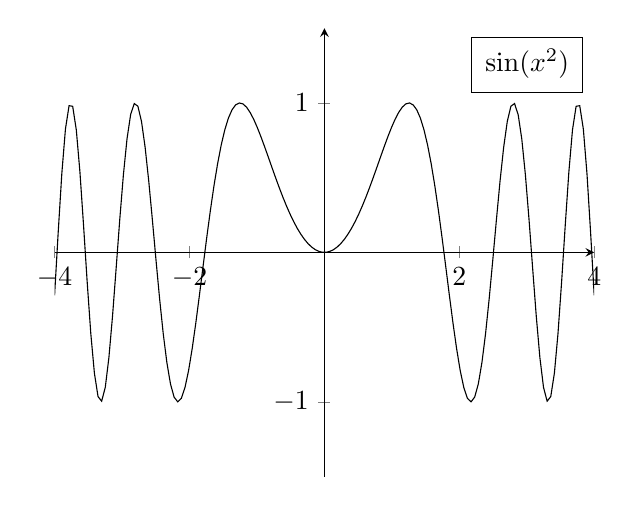
\begin{tikzpicture}
					\begin{axis} [
						axis lines = center,
						axis on top=true,
						legend style={empty legend},
						ymin = -1.5,
						ymax = 1.5
					]
						\addplot[domain=-4:4, samples=150] {sin(deg(x^2))};
						\addlegendentry{\raisebox{.5ex}{$\sin({x^2})$}}
					\end{axis}
				\end{tikzpicture}
			}
			\caption{No unif. cont.}
		\end{subfigure}
		\begin{subfigure}{.24\textwidth}
			\centering
			\resizebox{\linewidth}{!}{
				\begin{tikzpicture}
					\begin{axis} [
						axis lines = center,
						axis on top=true,
						legend style={empty legend},
						ymin = -1.5,
						ymax = 1.5
					]
						\addplot[domain=-4:4, samples=150] {(1/x)*sin(deg(x^2))};
						\addlegendentry{\raisebox{.5ex}{$\frac{1}{x}\sin({x^2})$}}
					\end{axis}
				\end{tikzpicture}
			}
			\caption{Sì unif. cont.}
		\end{subfigure}
	\end{figure}
\end{example}
\begin{exercise}
	\label{ex:cont_unif_cont_comparision}
	Confrontare la \fullref{prop:funz_cont_per_succ_in_ins} con la \fullref{def:funz_unif_cont}
	\begin{solution}
		In \fullref{prop:funz_cont_per_succ_in_ins} si definiva la continuità della funzione sull'insieme applicando la \fullref{def:funz_cont} a ogni $x_0 \in A$, cioè ogni punto di $A$. Questo non ha particolari implicazioni sul comportamento della funzione, informa solamente sulla continuità in ogni punto di $A$.\\
		\fullref{def:funz_unif_cont} invece prevede, per definizione, la possibilità di scegliere un qualsiasi $x_0$ quando $\varepsilon$ è già stato scelto. Ciò implica che $\varepsilon$ debba essere valido per ogni $x_0 \in A$, non scelto \textit{a priori}.
	\end{solution}
\end{exercise}
\begin{proposition}
	\label{prop:if_unif_cont_then_conf}
	Siano $(X,d_X)$ e $(Y,d_Y)$ spazi metrici. Sia $f:A \to Y$ con $A \subseteq X$.\\
	Se $f$ è \textbf{uniformemente continua} in $A$, allora $f$ è \textbf{continua} in $A$.
	\begin{proof}
		Deriva da \fullref{ex:cont_unif_cont_comparision} in quanto, se è possibile scegliere un qualsiasi $x_0$ quando $\varepsilon$ è già stato fissato, sicuramente sarà possibile fare questa scelta anche in ordine inverso (la continuità è condizione meno stringente).
	\end{proof}
\end{proposition}
\begin{exercise}
	Siano $(X,d_X)$ e $(Y,d_Y)$ spazi metrici e $k \in Y$. Data $f:\; X \to Y$ definita da $f(x) = k \quad \forall x \in X$.\\
	Dimostrare che $f$ è uniformemente continua.
	% TODO solution
\end{exercise}
\begin{exercise}
	Formulare e dimostrare il teorema sulla uniforme continuità della composizione di funzioni uniformemente continue in spazi metrici.
	% TODO solution
\end{exercise}
\begin{example}
	Sia $f:\; \R \to \R$ data da $f(x) = x^2$. $f$ è continua in $\R$, ma \textit{non} è uniformemente continua in $\R$
\end{example}
\begin{exercise}
	Esibire esempi di funzioni $f:\; \R \to \R$ che siano limitate/illimitate ed uniformemente continue.
\end{exercise}
\begin{example}
	Sia $f:\; \intervalopcl{0}{1} \to \R$ data da $f(x) = \sin(\frac{1}{x})$.\\
	In $\intervalopcl{0}{1}$, $f$ è continua e limitata, ma non è uniformemente continua.
\end{example}

\begin{theorem}[di Cantor]
	\label{teo:cantor}
	Siano $(X,d_X)$ e $(Y,d_Y)$ spazi metrici e sia $f:K \to Y$ con $K \subseteq X$.
	\begin{equation*}
		\left.
		\begin{array}{l}
		K \text{ \textbf{Compatto}} \\
		f \text{ \textbf{Continua} su } K
		\end{array}
		\right\} \implies
		f \text{ \textbf{Uniformemente Continua} su } K
	\end{equation*}
	\begin{proof} Per assurdo, negando la conclusione
		\begin{align*}
			&f \text{ non è uniformemente continua in } K\\
			\implies & \exists \varepsilon > 0 \text{ tale che } \forall \delta > 0 \quad \exists x', x'' \in K \text{ con } d(x', x'') < \delta \text{ e } d \bigl( f(x'), f(x'') \bigr) > \varepsilon
			\intertext{Ponendo $\delta = \frac{1}{n+1}$ si passa alla successione convergente a $0$, dunque compatibile con il $\delta$ precedente}
			\implies & \exists \varepsilon > 0 \text{ tale che } \forall n \in \N \quad \exists x_n', x_n'' \in K \text{ con } \underbrace{d(x_n', x_n'') < \frac{1}{n+1}}_{\text{(1)}} \text{ e } \underbrace{d \bigl( f(x_n'), f(x_n'') \bigr) > \varepsilon}_{\text{(2)}} \tageq\label{eq:th_cantor}
		\end{align*}
		Essendo $K$ compatto per ipotesi, per le due successioni $x_n'$ e $x_n''$ esistono due sottosuccessioni $x_{n_k}'$ e $x_{n_k}''$ convergenti a $x_\infty', x_\infty'' \in K$.\\
		Da (1) di \cref{eq:th_cantor} si sa che $\lim\limits_{n \to +\infty} d(x_n', x_n'') = 0$, dunque $x_\infty' = x_\infty''$ per $n \to +\infty$\\
		Da (2) di \cref{eq:th_cantor}, d'altro canto, è esplicitato che $d \bigl( f(x_n'), f(x_n'') \bigr)$ rimane sempre $> \varepsilon$ strettamente positivo, dunque è negata la \fullref{def:funz_cont} in $x_\infty' = x_\infty''$. Così è negata l'ipotesi sulla continuità della funzione.
	\end{proof}
\end{theorem}
\begin{proposition}
	Siano $(X,d_X)$ e $(Y,d_Y)$ spazi metrici, $A \subseteq X$ e $f:A \to Y$ \textbf{Uniformemente Continua} su $A$. Allora, per ogni successione $x:\N \to X$ \textbf{di Cauchy} in $X$, la successione $f \circ x$ delle immagini $f(x_n)$ \textbf{è di Cauchy} in $Y$.
	\begin{proof}
		Omessa.
	\end{proof}
\end{proposition}
\begin{proposition}
	Siano $(X,d_X)$ e $(Y,d_Y)$ spazi metrici, $A \subseteq X$ e $f:A \to Y$ \textbf{Uniformemente Continua} su $A$. Allora esiste un'unica funzione
	\[\overline{f}: \overline{A} \to Y\]
	continua su $\overline{A}$ e tale che $f_{|A} = f$ (cioè la $f$ ristretta ad $A$, dove definita, corrisponde a $f$)
	\begin{proof}
		Omessa.
	\end{proof}
\end{proposition}

\subsection{Lipschitzianità}
\begin{definition}[Funzione Lipschitziana]
	\label{def:lips}
	Siano:
	\begin{itemize}[noitemsep]
		\item $(X,d_X)$, $(Y,d_Y)$ spazi metrici
		\item $A \subseteq X$
		\item $f:A \to Y$
	\end{itemize}
	Allora
	\begin{equation*}
		\begin{gathered}
			f \text{ è \textbf{Lipschitziana}}\\
			\bydef\\
			\exists L > 0:\; \forall x',\,x'' \in X, \quad d_Y\bigl(f(x''),f(x')\bigr) \leq L \cdot d_X(x'',x')
		\end{gathered}
	\end{equation*}
	\begin{note}
		La costante $L$ sopra introdotta non è univocamente determinata. Nei risultati seguenti non sarà mai rilevante \textit{il valore} di $L$, ma il fatto stesso che $L$ esista.
	\end{note}
\end{definition}
\begin{definition}[Costante di Lipschitz]
	\label{def:cost_lips}
	Fissate le distanze $d_X$ e $d_Y$ e la funzione $f$, allora la più piccola $L$ positiva soddisfacente
	\[d_Y\bigl(f(x''),f(x')\bigr)\leq L \cdot d_X(x'',x') \qquad \forall x',x'' \in X\]
	si definisce \textbf{Costante di Lipschitz} della funzione $f$ in $X$
\end{definition}
\begin{example}
	\label{ex:lips_graphs}
	~
	\begin{figure}[H]
		\begin{subfigure}{.24\textwidth}
			\centering
			\resizebox{\linewidth}{!}{
				\begin{tikzpicture}
					\begin{axis} [
						axis lines = center,
						axis on top=true,
						legend style={empty legend}
					]
						\addplot [domain=-3:-2.5,samples=10] {-x-2};
						\addplot [domain=-2.5:-1.5,samples=10] {x+3};
						\addplot [domain=-1.5:-.5,samples=10] {-x};
						\addplot [domain=-.5:1,samples=10] {x+1};
						\addplot [domain=1:1.5,samples=10] {-x+3};
						\addplot [domain=1.5:3,samples=10] {x};
					\end{axis}
				\end{tikzpicture}
			}
			\caption{Sì lips.}
		\end{subfigure}
		\begin{subfigure}{.24\textwidth}
			\centering
			\resizebox{\linewidth}{!}{
				\begin{tikzpicture}
					\begin{axis} [
						axis lines = center,
						axis on top=true,
						legend style={empty legend}
					]
						\addplot [domain=-2:2,samples=100] {x^2};
						\addlegendentry{\raisebox{.5ex}{$x^2$}}
					\end{axis}
				\end{tikzpicture}
			}
			\caption{No lips.}
		\end{subfigure}
		\begin{subfigure}{.24\textwidth}
			\centering
			\resizebox{\linewidth}{!}{
				\begin{tikzpicture}
					\begin{axis} [
						axis lines = center,
						axis on top=true,
						ymin = -2,
						ymax = 2
					]
						\addplot[domain=-2:0, samples=10] {1};
						\addplot[domain=0:2, samples=10] {-1};
						\addplot [only marks, mark=*] coordinates{(0,-1)};
						\addplot [fill=white, only marks,mark=*] coordinates{(0,1)};
					\end{axis}
				\end{tikzpicture}
			}
			\caption{No lips.}
		\end{subfigure}
		\begin{subfigure}{.24\textwidth}
			\centering
			\resizebox{\linewidth}{!}{
				\begin{tikzpicture}
					\begin{axis} [
						axis lines = center,
						axis on top=true,
						legend style={empty legend}
					]
						\addplot [domain=0:.2,samples=100,smooth] {sqrt(x)};
						\addplot [domain=.2:3,samples=50] {sqrt(x)};
						\addlegendentry{\raisebox{.5ex}{$\sqrt{x}$}}
					\end{axis}
				\end{tikzpicture}
			}
			\caption{No lips.\newline (Sì unif. cont.)}
		\end{subfigure}
	\end{figure}
\end{example}
\begin{example}
	Sono dati gli spazi metrici $(X,d_X)$ e $(Y,d_Y)$ ed una funzione Lipschitziana $f: X \to Y$.\\
	Determinare una nuova distanza $\delta_X$ su $X$ che sia equivalente a $d_X$ ed in modo che la costante di Lipschitz di $f$ rispetto a $\delta_X$ sia minore o uguale ad $1$.
	% TODO solution
\end{example}
\begin{example}
	Sono dati gli spazi metrici $(X,d_X)$ e $(Y,d_Y)$ ed una funzione Lipschitziana $f: X \to Y$.\\
	Determinare una nuova distanza $\delta_Y$ su $Y$ che sia equivalente a $d_Y$ ed in modo che la costante di Lipschitz di $f$ rispetto a $\delta_Y$ sia minore o uguale ad $1$.
	% TODO solution
\end{example}
\begin{exercise}
	Sia $f: \R \to \R$. Come si fa a capire se $f$ è Lipschitziana o no dal suo grafico?
\end{exercise}

\begin{proposition}
	\label{prop:convesso_deriv_par_lim_allora_lips}
	Siano $A \subseteq \R^n$ un insieme \textbf{Convesso} (da \fullref{def:convesso}) e $f \in \cntclass{1}(A;\R)$ (da \fullref{def:cnt_class_1}). Se tutte le \textbf{Derivate Parziali} sono \textbf{limitate} in $A$ , allora $f$ è \textbf{Lipschitziana}.
	\begin{proof}
		Segue direttamente da \fullref{def:convesso} e \fullref{teo:accresc_fin}.
	\end{proof}
\end{proposition}

\begin{proposition}
	\label{prop:se_lips_allora_unif_cont}
	Sia $f: X \to Y$ una funzione \textbf{Lipschitziana}. Allora $f$ è \textbf{Uniformemente Continua} su $X$.
	\begin{proof}
		Dall'ipotesi di Lipschitzianità, applicando la \fullref{def:lips}, si sa per certo che
		\[d_Y\bigl(f(x''),f(x')\bigr) \leq L \cdot d_X(x'',x')\]
		Posti ora
		\begin{itemize}
			\item $d_X(x'',x') < \delta$ senza perdere generalità (il $\delta$ nella unif. continuità è a scelta)
			\item $\delta = \frac{\varepsilon}{L}$ come semplice posizione
		\end{itemize}
		Si ottiene
		\[d_Y\bigl(f(x''),f(x')\bigr) \leq L \cdot d_X(x'',x') < L \cdot \delta = L \cdot \frac{\varepsilon}{L} = \varepsilon\]
		Da cui, prendendo il primo e l'ultimo membro,
		\[d_Y\bigl(f(x''),f(x')\bigr) < \varepsilon\]
		che è la condizione di uniforme continuità.
	\end{proof}
\end{proposition}
\begin{example}
	La funzione
	\[\funcdef{f}{\intervalclop{0}{+\infty}}{\R}{x}{\sqrt{x}}\]
	è uniformemente continua ma non è Lipschitziana. Vedere grafico in \fullref{ex:lips_graphs}
\end{example}
\begin{example}
	La funzione
	\[\funcdef{f}{\R}{\R}{x}{\begin{cases}
		\begin{array}{ll}
			x \cdot \sin \left(\frac{1}{x}\right) & \text{se } x \neq 0\\
			0 & \text{se } x = 0\\
		\end{array}
	\end{cases}}\]
	è uniformemente continua ma non è Lipschitziana.
\end{example}
\begin{example}
	La funzione
	\[\funcdef{f}{\intervalclop{0}{+\infty}}{\R}{x}{x^2}\]
	è di classe $\cntclass{\infty}$ ma non è Lipschitziana. Vedere grafico in \fullref{ex:lips_graphs}
\end{example}
\begin{example}
	La funzione
	\[\funcdef{f}{\intervalclop{0}{+\infty}}{\R}{x}{\abs{x}}\]
	è Lipschitziana ma non è derivabile in $0$.
\end{example}
\begin{exercise}
	\label{ex:comp_funz_lips}
	La composizione di funzioni Lipschitziane è Lipschitziana?\\
	Per funzioni reali di variabile reale, la somma/il prodotto di funzioni Lipschitziane è una funzione Lipschitziana?\\
	Enunciare formalmente e dimostrare.
	% TODO solution
\end{exercise}

\begin{proposition}
	Siano $(X,d_X)$ e $(Y,d_Y)$ spazi metrici. Sia $f:A \to \R^n$ con $A \subseteq X$.
	\begin{equation*}
		f \text{ è \textbf{Lipschitziana}} \iff \text{\textbf{ogni componente di} } f \text{ \textbf{è Lipschitziana}}
	\end{equation*}
	\begin{proof}
		Immediata.
		% TODO actual proof
	\end{proof}
\end{proposition}

\begin{definition}[Norma di Matrice]
	\label{def:norm_matr}
	Sia $A \in \mat (m \times n)$. \textbf{Norma} di $A$ è la quantità
	\[\norm{A} = \;\; \max\limits_{\raisebox{-1ex}{${\scriptstyle x \in \overline{B(0,1)} }$}} \; \norm{A \; x}\]
	con $x$ vettore $\in \R^n$ e $A \; x \in \R^m$ risultato del prodotto righe per colonne.
\end{definition}
\begin{exercise}
	Verificare che la norma introdotta in \fullref{def:norm_matr} soddisfi alle condizioni della \fullref{def:norma} con $V = \mat (m \times n)$
\end{exercise}
\begin{exercise}
	\label{ex:matr_form_alt}
	Con la notazione della \fullref{def:norm_matr}, verificare le seguenti uguaglianze
	{
	\renewcommand*{\arraystretch}{1.5} % To improve the spacing of this array
	\begin{equation*}
		\begin{array}{rll}
			\norm{A}	& =\sup\limits_{\raisebox{-1ex}{${\scriptstyle x \in \overline{B(0,1)} }$}} \; \norm{A \; x}	& =\sup\limits_{x \in B(0,1)} \; \norm{A \; x}\\
						& =\max\limits_{\norm{x} = 1} \; \norm{A \; x}													& =\sup\limits_{\norm{x} = 1} \; \norm{A \; x}\\
						& =\sup\limits_{x \in \R^n \setminus \brackets{0}} \frac{\norm{A \; x}}{\norm{x}}
		\end{array}
	\end{equation*}
	}
	% TODO solution
\end{exercise}

\begin{proposition}
	\label{prop:proprieta_norm_matr}
	Sia $A \in \mat(m \times n)$. Allora
	\[\norm{A \; x} \leq \norm{A} \cdot \norm{x}\]
	\begin{proof}
		Sia $x = 0$ la tesi è immediata.\\
		Sia $x \neq 0$, allora
		\begin{align*}
			\norm{A \; x} &= \norm{A \; x \cdot \frac{\norm{x}}{\norm{x}}} = \norm{\norm{x} \cdot \left( A \frac{x}{\norm{x}} \right)}\\
			&= \norm{x} \cdot \norm{A \frac{x}{\norm{x}}}
			\intertext{Essendo $\frac{x}{\norm{x}}$ il versore di $x$, esso ha, per definizione, norma unitaria e, grazie a \fullref{ex:matr_form_alt}, si sa che $\norm{A} \leq \sup\limits_{\norm{x} = 1} \; \norm{A \; x}$, dunque}
			&\leq \norm{A} \cdot \norm{x}
		\end{align*}
	\end{proof}
\end{proposition}
\begin{exercise}
	Esibire una matrice $A \in \mat(2 \times 3)$ tale che $\norm{A} = 2$
	% TODO solution
\end{exercise}
\begin{exercise}
	Sia $f:\R^n \to \R^n$ una funzione lineare. Allora è Lipschitziana (rispetto alla metrica Euclidea). Suggerimento: utilizzare la \fullref{prop:proprieta_norm_matr}
	\begin{note}
		In spazi più generali di $\R^n$ (spazi di dimensione \textit{infinita}) l'affermazione contenuta in questo esercizio può essere falsa. Vedasi \fullref{prop:dist_lin_non_cont}
	\end{note}
	% TODO solution
\end{exercise}
\begin{exercise}
	Se $A$ e $B$ sono matrici tali che se ne possa fare il prodotto (regole del prodotto righe per colonne), dimostrare che
	\[\norm{A \cdot B} \leq \norm{A} \cdot \norm{B}\]
	% TODO solution
\end{exercise}

\newpage
\section{Il Teorema delle Contrazioni}
\begin{definition}[Contrazione]
	\label{def:contrazione}
	Sia $(X, d)$ uno spazio metrico. Si dice \textbf{Contrazione} una funzione $T:\; X \to X$ soddisfacente a:
	\begin{equation}
		\label{eq:def_contrazione}
		\exists K \in [0, 1[ \text{ tale che } \forall x',x'' \in X \quad \text{vale} \quad d_X \bigl( T(x''), T(x') \bigr) \leq K \cdot d_X(x'', x')
	\end{equation}
	Una contrazione è quindi una funzione con insieme di partenza e di arrivo coincidenti e Lipschitziana con costante di Lipschitz strettamente minore di $1$.\\
	È generalmente inutile considerare contrazioni definite tra spazi diversi. Infatti, data una funzione $T: X \to Y$ Lipschitziana, sarebbe sempre possibile riscalare la distanza in uno dei due spazi $X$ o $Y$ per ottenere una costante di Lipschitz minore di $1$.
	\begin{note}
		D'ora in poi si utilizzerà spesso la notazione $Tx$ per intendere $T(x)$
	\end{note}
\end{definition}
\begin{example}[Esempi di Contrazioni]\leavevmode\vspace*{-\baselineskip}
	\begin{enumerate}
		\item $f: \R \to \R$ data da $f(x) = \frac{x}{2}$. $f$ è una contrazione.
		\item $f: \intervalclose{0}{2} \to \intervalclose{0}{2}$ data da $f(x) = 1 + \frac{x}{2}$. $f$ è una contrazione
		\item $f: \R^2 \to \R^2$ data da $f(x,y)=
			\begin{bmatrix}
				\frac{1}{3} & 0\\[1ex]
				0 & \frac{1}{5}
			\end{bmatrix} \cdot
			\begin{bmatrix}
				x\\[1ex]
				y
			\end{bmatrix}$. $f$ è una contrazione
	\end{enumerate}
\end{example}
\begin{exercise}
	La composizione di contrazioni è una contrazione. Enunciare formalmente e dimostrare.\\
	Esibire esempi che mostrino come la somma ed il prodotto di contrazioni possano non essere contrazioni.
	\begin{solution}\hfill\\
		Sia $(X, d)$ uno spazio metrico, siano $f,g:X \to X$ \textbf{due contrazioni} in $X$. Allora $f\circ g$ è una \textbf{contrazione}
		\begin{proof}
			\renewcommand\qedsymbol{$\square$}
			Sappiamo che:
			\begin{equation*}
				\begin{gathered}
					\forall x',x'' \in X,\; d \bigl( f(x''), f(x') \bigr) \leq K_f \cdot d(x'', x')\\
					\forall x',x'' \in X,\; d \bigl( g(x''), g(x') \bigr) \leq K_g \cdot d(x'', x').
				\end{gathered}
			\end{equation*}
			$f \circ g=f\bigl( g(x) \bigr)$, quindi presi $x',x''\in X$ si ha
			\[d \Bigl( f\bigl(g(x'')\bigr), f\bigl(g(x')\bigr) \Bigr) \leq K_f \cdot d \bigl( g(x''), g(x') \bigr) \leq K_f K_g \cdot d(x'',x')\]
		\end{proof}
		\noindent Esempi: % TODO esempi
	\end{solution}
\end{exercise}

\begin{proposition}
	\label{prop:se_Df_leq_k_allora_f_contr}
	Sia $f \in \cntclass{1}(\R^n;\R^n)$ (da \fullref{def:cnt_class_1}). Se esiste $k \in \intervalclop{0}{1}$ tale che per ogni $x \in \R^n$ vale $\norm{Df(x)} < k$, allora $f$ è \textbf{Contrazione}.
	\begin{proof}
		Segue dal \fullref{teo:accresc_fin}
	\end{proof}
\end{proposition}

\begin{definition}[Punto Fisso]
	\label{def:punto_fisso}
	Sia $X$ un insieme e $f: X \to X$. Un \textbf{Punto Fisso} di $f$ è un elemento $x \in X$ tale che:
	\[x=f(x)\]
\end{definition}

\begin{theorem}[delle Contrazioni]\leavevmode\vspace*{-\baselineskip}
	\label{teo:contrazioni}
	\begin{note}
		Questo teorema è anche noto come \textit{Teorema di Banach-Cacioppoli}
	\end{note}
	Sia $(X, d)$ uno spazio metrico e $T: X \to X$. Allora
	\begin{equation*}
		\left.
			\begin{array}{l}
				X \text{ \textbf{Completo}}\\
				T \text{ \textbf{Contrazione}}
			\end{array}
		\right\}
		\implies
		\exists! \; x_* \in X: \quad T(x_*) = x_*
	\end{equation*}
	Cioè esiste un \textbf{unico Punto Fisso} di $T$ in $X$.
	\begin{proof}
		La dimostrazione si divide in 3 passaggi
		\begin{enumerate}
			\item \textit{Individuazione di una Successione di Cauchy}\\
				Dato un generico $x_0 \in X$ si costruisce una successione $x$ nel seguente modo:
				\begin{equation}
					\label{eq:teo_contraz_succ}
					\begin{matrix}x_0 \in X & \quad & x_1 = T(x_0) & \quad & x_2 = T(x_1) & \quad & \dotsc & \quad & x_{n+1} = T(x_n)\end{matrix}
				\end{equation}
				La  successione $x:\N \to X$ è sicuramente ad elementi in $X$ in quanto $T$, contrazione, è per definizione $T: X \to X$. È necessario dimostrare che la $x$ sia di Cauchy (\fullref{def:succ_cau}) cioè che:
				\[\forall \varepsilon > 0\quad \exists \nu \in \N:\; \forall n,m > \nu \text{ vale } d(x_n, x_m) < \varepsilon\]
				Presi ora due qualunque $n$ e $m$ e sfruttando il modo in cui è definita la successione $x$:
				\begin{align*}
					d(x_n, x_m) &= d \bigl( T(x_{n-1}), T(x_{m-1}) \bigr)
					\shortintertext{Grazie al fatto che $T$ è contrazione, per definizione esiste un $K \in \intervalclop{0}{1}$ per cui}
					&\leq K \cdot d(x_{n-1}, x_{m-1})
					\shortintertext{Ripetendo gli ultimi due passaggi, si continua}
					&= d \bigl( T(x_{n-2}), T(x_{m-2}) \bigr)\\
					&\leq K^2 \cdot d(x_{n-2}, x_{m-2})
					\shortintertext{Ipotizzando ora $n < m$, sicuramente dopo un $n$ numero di passi analoghi si arriverà a $0$}
					&\leq K^n \cdot d(x_0, x_{m-n})
				\end{align*}
				Quindi, andando dal primo all'ultimo passaggio, si è ottenuta la disuguaglianza
				\begin{equation}
					\label{eq:teo_contraz_disug_dist_mn}
					d(x_n, x_m) \leq K^n \cdot d(x_0, x_{m-n})
				\end{equation}
				Ora, applicando ripetutamente la disuguaglianza triangolare al secondo membro della \cref{eq:teo_contraz_disug_dist_mn}
				\begin{align*}
					K^n \cdot d(x_0, x_{m-n}) &\leq K^n \cdot \Bigl( d(x_0, x_1) + d(x_1, x_2) + \dotsc + d(x_{m-n-1}, x_{m-n}) \Bigr)
					\shortintertext{Applicando ora quanto ottenuto in \cref{eq:teo_contraz_disug_dist_mn} a tutti gli addendi}
					&\leq K^n \cdot \Bigl( K^0 \cdot d(x_0, x_1) + K^1 \cdot d(x_0, x_1) + \dotsc + K^{m-n-1} \cdot d(x_0, x_1) \Bigr)\\
					&\leq K^n \cdot (1 + K + \dotsc + K^{m-n-1}) \cdot d(x_0, x_1)
				\end{align*}
				Quindi riassumento, partendo dal primo membro dalla \cref{eq:teo_contraz_disug_dist_mn}, si è arrivati a
				\begin{equation}
					\label{eq:teo_contraz_disug_dist_mn_fin}
					d(x_n, x_m) \leq K^n \cdot (\underbrace{1 + K + \dotsc + K^{m-n-1}}_{\text{(1)}}) \cdot d(x_0, x_1)
				\end{equation}
		
				Posta ora la (1) di \cref{eq:teo_contraz_disug_dist_mn_fin} come $s$ si ha:
				\[s = 1 + K + \dotsc + K^{m-n-1} \qquad \text{e, moltiplicando per } K \text{,} \qquad K \cdot s = K + K^2 + \dotsc + K^{m-n}\]
				Da cui, eseguendo la differenza tra $s$ e $K \cdot s$
				\begin{align*}
					&s - K \cdot s\\
					= &(1 + \cancel{K} + \cancel{\dotsc} + K^{m-n-1}) - (\cancel{K} + \cancel{K^2} + \cancel{\dotsc} + K^{m-n})\\
					= &1 - K^{m-n}
				\end{align*}
				si ottiene l'equivalenza
				\begin{align*}
					s - K \cdot s &= 1 - K^{m-n}\\
					s (1 - K) &= 1 - K^{m-n}\\
					s &= \frac{1 - K^{m-n}}{1 - K}
				\end{align*}
				Sostituendo la formulazione di $s$ appena trovata in \cref{eq:teo_contraz_disug_dist_mn_fin} si ottiene
				\begin{equation}
					\label{eq:teo_contraz_disug_s}
					d(x_n, x_m) \leq K^n \cdot \frac{1 - K^{m-n}}{1 - K} \cdot d(x_0, x_1)
				\end{equation}
				Essendo $K \in \intervalclop{0}{1}$, eseguendone l'elevamento a potenza otterrò un numero ancor più piccolo. È dunque certo che
				\[1 - K^{m-n} \geq 1 - K \implies \frac{1 - K^{m-n}}{1 - K} \leq 1\]
				per cui è sicuramente possibile minorare la \cref{eq:teo_contraz_disug_s} che diventa
				\begin{equation}
					\label{eq:teo_contraz_disug_dist_01}
					d(x_n, x_m) \leq K^n \cdot d(x_0, x_1)
				\end{equation}
				\vspace*{-4ex}
				\begin{note}
					\hypertarget{note:teo_contraz_note}{}
					La \cref{eq:teo_contraz_disug_dist_01}, per come è scritta, fornisce un importante risultato. Grazie a questa equazione, noto $n$ e calcolando solo la distanza tra gli elementi $0$ ed $1$ della successione (facilmente individuabili) si ha un limite superiore per la $d(x_n, x_m) \; \forall n,m$. Non sarebbe stato invece possibile calcolare la $d(x_0, x_{n-m})$ trovata ancora prima.
				\end{note}
				Questa minorazione permette di verificare la definizione di successione di Cauchy, dunque la $x$ definita in \cref{eq:teo_contraz_succ} è di Cauchy.
				\qed
			\item \textit{Individuazione del Punto Fisso}\\
				La successione $x$ definita in \cref{eq:teo_contraz_succ}, essendo stata dimostrata di Cauchy nel passo precedente, per \fullref{def:completo} ammette sicuramente $\lim\limits_{n \to +\infty} x_n = x_* \in X$. Inoltre
				\[
					T \text{ Contrazione}
					\quad \overset{
						\mathclap{
							\rule[-\baselineskip]{0pt}{\baselineskip}
							\text{
								\begin{tabular}{c}
									Come da\\[-1ex]
									\fullref{def:contrazione}
								\end{tabular}
							}
						}
					}{\implies} \quad T \text{ Lipschitziana}
					\quad \overset{
						\mathclap{
							\rule[-\baselineskip]{0pt}{\baselineskip}
							\text{
								\begin{tabular}{c}
									Per\\[-1ex]
									\fullref{prop:se_lips_allora_unif_cont}
								\end{tabular}
							}
						}
					}{\implies} \quad T \text{ Unif. Cont.}
					\quad \overset{
						\mathclap{
							\rule[-\baselineskip]{0pt}{\baselineskip}
							\text{
								\begin{tabular}{c}
									Per\\[-1ex]
									\fullref{prop:if_unif_cont_then_conf}
								\end{tabular}
							}
						}
					}{\implies} \quad T \text{ Continua}
				\]
				Posto quindi
				\begin{align*}
					T(x_*) &= T \bigl( \; \lim\limits_{n \to +\infty} x_n \; \bigr)
					\shortintertext{Grazie alla continuità di $T$}
					&= \lim\limits_{n \to +\infty} \bigl(T(x_n)\bigr)
					\shortintertext{Dunque, per come è definita $x$}
					&= \lim\limits_{n \to +\infty} ( x_{n+1} )\\
					&= x_*
				\end{align*}
				\qed
			\item \textit{Dimostrazione unicità punto fisso}\\
				Si suppone non sia unico
				\[x_0, y_0 \in X \;\; x_0 \neq y_0 \qquad T(x_0) = x_0,\; T(y_0) = y_0\]
				Calcolando la distanza tra i due punti, sfruttando il fatto che siano punti fissi per definizione ed, infine, essendo $T$ contrazione si ottiene
				\begin{equation*}
					\begin{gathered}
						d(x_0, y_0) = d\bigl( T(x_0), T(y_0) \bigr) \leq K \cdot d(x_0, y_0)\\
						d(x_0, y_0) - K \cdot d(x_0, y_0) \leq 0
					\end{gathered}
				\end{equation*}
				\begin{equation}
					\label{eq:teo_contraz_unicita}
					(1-K) \bigl( d(x_0, y_0) \bigr) \leq 0
				\end{equation}
				Però
				\begin{itemize}
					\item $1-k > 0$ strettamente positivo perché, per \fullref{def:contrazione} $k \in \intervalclop{0}{1}$
					\item $d(x_0, y_0) \geq 0$ per \fullref{def:sp_metrico}
				\end{itemize}
				Allora deve essere per forza $d(x_0, y_0) = 0$ per non contraddire la \cref{eq:teo_contraz_unicita}, dunque, per proprietà \ref{itm:dist_0_iff_x_uguale_y} delle distanze (\fullref{def:sp_metrico}), $x_0 = y_0$.
				% No need for QED symbol here since one is provided by the proof environment
		\end{enumerate}
	\end{proof}
\end{theorem}
\begin{exercise}
	I passaggi da \cref{eq:teo_contraz_disug_dist_mn} a \cref{eq:teo_contraz_disug_dist_01} sono necessari?
	\begin{solution}
		Vedere \hyperlink{note:teo_contraz_note}{nota alla dimostrazione del \fullref*{teo:contrazioni}}
	\end{solution}
\end{exercise}
\begin{example}
	Se $X$ \textit{non} è completo:\\
	Siano $X = \intervalopen{0}{1}$ e $T: X \to X$ data $T(x) = \frac{x}{2}$. $T$ è una contrazione senza punti fissi in $X$
\end{example}
\begin{example}
	Se $T$ è \textit{quasi} una contrazione possono non esserci punti fissi:\\
	Sia $X = \R$ e sia $T:X \to X$ data da $T(x) = x + \frac{\pi}{2} - \arctan x$. Grazie al Teorema di Lagrange (da Analisi 1, essendo in $\R$) si può facilmente dimostrare che $\forall x', x'' \in X$
	\[\abs{T(x'') - T(x')} < \abs{x'' - x'}\]
	però $T$ non è una contrazione ed infatti non ammette punti fissi.
\end{example}
\begin{example}
	Se $T$ è \textit{quasi} una contrazione possono esserci infiniti punti fissi:\\
	Sia $X = \R$ e sia $T:X \to X$ data da $T(x) = x$. Evidentemente
	\[\abs{T(x'') - T(x')} = \abs{x'' - x'}\]
	e $T$ ammette infiniti punti fissi.
\end{example}
\begin{exercise}
	Sia $f \intervalclose{0}{1} \to \intervalclose{1}{2}$ data da $f(x) = 1 + \frac{x}{2}$\\
	$f$ è una funzione Lipschitziana con costante di Lipschitz $\frac{1}{2}$ definita tra spazi metrici completi ma senza punti fissi. È in contraddizione con il \fullref{teo:contrazioni}?
	% TODO solution
\end{exercise}
\begin{exercise}
	Sia $f:\R \to \R$ derivabile su $\R$ e tale che $f'(x) \leq \frac{1}{2} \quad \forall x \in \R$.\\
	Dimostrare che allora esiste un unico $x_* \in \R$ tale che $f(x_*) = x_*$
	\begin{solution}
		$\R$ è Completo come da \fullref{ex:sp_metr_compl_e_non}, inoltre la $f$ è Contrazione per \fullref{prop:se_Df_leq_k_allora_f_contr}, dunque è possibile applicare il \fullref{teo:contrazioni} ed arrivare alla tesi.
	\end{solution}
\end{exercise}

\begin{observation}
	\label{obs:contr_con_para}
	È utile considerare \textbf{contrazioni} che dipendono da uno o più \textbf{parametri}. Siano $(X,d)$ uno spazio metrico completo, $P$ un \textbf{insieme} di parametri e $T:X \times P \to X$.\\
	Grazie al \fullref{teo:contrazioni} è data l'esistenza di un punto fisso di $T$ indipendentemente dal parametro. È dunque possibile definire una funzione $\varphi: P \to X$ che ad ogni parametro $p \in P$ associa $\varphi(p)$, unico punto fisso della contrazione.\\
	In generale, la regolarità della funzione $\varphi$ è la stessa con cui $T$ dipende dal parametro $p$. Vedasi \fullref{teo:contrazioni_con_para} e \fullref{teo:contr_con_para_lips_definisce_funz_lips}
\end{observation}

\begin{definition}[Contrazione con Parametro]
	\label{def:contrazione_parametro}
	Siano $(X,d)$ uno \textbf{Spazio Metrico} e $P$ un \textbf{Insieme}
	\begin{equation}
		\label{eq:contrazione_parametro}
		\begin{gathered}
			T \text{ è una \textbf{Contrazione} in } x \in X \text{ \textbf{Uniformemente} in } p \in P\\
			\bydef\\
			\exists K \in \intervalclop{0}{1}: \; \forall p \in P,\; \forall x', x'' \in X \quad \text{vale} \quad d \Bigl( T\bigl( x', p \bigr), T\bigl( x'', p \bigr) \Bigr) \leq K \cdot d(x', x'')
		\end{gathered}
	\end{equation}
	Cioè, indipendentemente da qualsiasi $p \in P$, la $T$ rimane contrazione.
\end{definition}

\cbstart
\begin{theorem}[delle Contrazioni con Parametro]
	\label{teo:contrazioni_con_para}
	Siano:
	\begin{itemize}[noitemsep]
		\item $(X,d_X)$ uno spazio metrico completo
		\item $(P,d_P)$ uno spazio metrico
		\item $T:X \times P \to X$ una contrazione in $x \in X$ uniformemente in $p \in P$
		\item $T$ continua
	\end{itemize}
	Allora $\forall p \in P$ esiste un unico punto fisso $x_p$ per la funzione $x \mapsto T(x,p)$ e la funzione $P \to X_p$ è continua.
	\begin{proof}
		Come già detto in \fullref{obs:contr_con_para}, il \fullref{teo:contrazioni} assicura l'esistenza di una funzione $\varphi: P \to X$ che ad ogni $p \in P$ associa un unico punto fisso di $x \mapsto T(x,p)$. $\varphi$ è continua. Infatti se $p_n \to p_0$
		\begin{align*}
					&d_X \bigl( \varphi(p_n), \varphi(p_0) \bigr) =
			\shortintertext{Essendo $\varphi(p_n)$ per definizione punto fisso di $T$ con parametro $p_n$}
			=\;\;	&d_X \Bigl( T \bigl( \varphi(p_n), p_n \bigr), T \bigl( \varphi(p_0), p_0 \bigr) \Bigr)
			\shortintertext{Applicando la disuguaglianza triangolare}
			\leq\;\;&d_X \Bigl( T \bigl( \varphi(p_n), p_n \bigr), T \bigl( \varphi(p_0), p_n \bigr) \Bigr) +
					d_X \Bigl( T \bigl( \varphi(p_0), p_n \bigr), T \bigl( \varphi(p_0), p_0 \bigr) \Bigr)
			\shortintertext{Con la definizione di contrazioni}
			\leq\;\;&K \cdot d_X \bigl( \varphi(p_n), \varphi(p_0) \bigr) +
					d_X \Bigl( T \bigl( \varphi(p_0), p_n \bigr), T \bigl( \varphi(p_0), p_0 \bigr) \Bigr)
		\end{align*}
		Dunque
		\[d_X \bigl( \varphi(p_n), \varphi(p_0) \bigr) \leq K \cdot d_X \bigl( \varphi(p_n), \varphi(p_0) \bigr) + d_X \Bigl( T \bigl( \varphi(p_0), p_n \bigr), T \bigl( \varphi(p_0), p_0 \bigr) \Bigr)\]
		Da cui, infine
		\[d_X \bigl( \varphi(p_n), \varphi(p_0) \bigr) \leq \frac{1}{1-K} \cdot d_X \Bigl( T \bigl( \varphi(p_0), p_n \bigr), T \bigl( \varphi(p_0), p_0 \bigr) \Bigr)\]
		Ed il secondo membro tende a $0$ per $n \to +\infty$ grazie alla continuità di $T$, quindi da \fullref{prop:cont_e_cont_per_succ} la $\varphi$ è continua.
	\end{proof}
\end{theorem}

\begin{definition}[Contrazione Lipschitziana in Parametro]
	\label{def:contr_lips_para}
	Siano $(X,d_X)$ e $(P,d_P)$ spazi metrici
	\begin{equation*}
		\begin{gathered}
			T \text{ è una \textbf{Contrazione} in } x \in X \text{ \textbf{Lipschitziana} in } p \in P\\
			\bydef\\
			\exists K \in \intervalclop{0}{1}, \exists L > 0: \; \forall p', p'' \in P, \forall x', x'' \in X \text{ vale}\\
			d_X \bigl( T( x', p'), T(x'', p'') \bigr) \leq K \cdot d_X(x', x'') + L \cdot d_P (p', p'')
		\end{gathered}
	\end{equation*}
	Cioè, si aggiunge la Lipschitzianità rispetto al parametro
\end{definition}
\begin{theorem}
	\label{teo:contr_con_para_lips_definisce_funz_lips}
	Siano:
	\begin{itemize}[noitemsep]
		\item $(X,d_X)$ uno spazio metrico completo
		\item $(P,d_P)$ uno spazio metrico
		\item $T:X \times P \to X$ una contrazione in $x \in X$ Lipschitziana in $p \in P$
	\end{itemize}
	Allora esiste un'unica funzione Lipschitziana $\varphi: P \to X$ tale che $\varphi(p)$ è l'unico punto fisso della funzione $x \mapsto T(x,p)$
	\begin{note}
		L'unicità del punto fisso implica automaticamente l'unicità della funzione $\varphi$
	\end{note}
	\begin{proof}
		Come già detto in \fullref{obs:contr_con_para}, il \fullref{teo:contrazioni} assicura l'esistenza di una funzione $\varphi: P \to X$ che ad ogni $p \in P$ associa un unico punto fisso di $x \mapsto T(x,p)$. $\varphi$ è Lipschitziana. Infatti
		\begin{align*}
			&d_X \bigl( \varphi(p'), \varphi(p'') \bigr) =
			\shortintertext{Essendo $\varphi(p)$ per definizione punto fisso di $T$ con parametro $p$}
			=\;\;	&d_X \Bigl( T \bigl( \varphi(p'), p' \bigr), T \bigl( \varphi(p''), p'' \bigr) \Bigr)
			\shortintertext{Applicando la \fullref{def:contr_lips_para}}
			\leq\;\;&K \cdot d_X \bigl( \varphi(p'), \varphi(p'') \bigr) + L \cdot d_P(p', p'')
		\end{align*}
		Dunque
		\[d_X \bigl( \varphi(p'), \varphi(p'') \bigr) \leq K \cdot d_X \bigl( \varphi(p'), \varphi(p'') \bigr) + L \cdot d_P(p', p'')\]
		Da cui, infine
		\[d_X \bigl( \varphi(p'), \varphi(p'') \bigr) \leq \frac{L}{1-K} \cdot d_P (p', p'')\]
		Che dimostra la Lipschitzianità di $\varphi$
	\end{proof}
\end{theorem}

\begin{exercise}
	Nel presente capitolo, ambientato in spazi metrici, non viene trattata la derivabilità del punto fisso rispetto al parametro. Perché?
	% TODO solution
\end{exercise}

\begin{definition}[Funzione Iterata]
	\label{def:iterata}
	Data $F:X \to X$, si dice \textbf{Funzione Iterata} $n$ volte di $F$ la $F^n$ che corrisponde all'\textbf{applicazione} $n$ volte di $F$ \textbf{su sè stessa}. Formalmente:
	\[f^{n+1} = f \circ f^n \quad \forall n \in \N\setminus\brackets{0}\]
	Se $n = 0$, per definizione, $f^0 = \mathrm{Id}_X$ con $\mathrm{Id}_X$ funzione identità su $X$
\end{definition}

\begin{theorem}[dell'Iterata Contrazione]
	\label{teo:iterata_contraz}
	Sia $(X,d_X)$ uno spazio metrico completo e sia $T:X \to X : \exists n \in \N, T^n$ \textbf{Iterata} è contrazione.\\
	Allora $T$ ammette un unico punto fisso in $X$
	\begin{note}
		La $n$ non è univocamente definita e non potrebbe esserlo.\\
		Se infatti $T^n$ è contrazione, allora anche $T^{2n},\, T^{3n},\, \cdots,\, T^{\alpha n}$ lo sono.
	\end{note}
	\begin{proof}
		Per il \fullref{teo:contrazioni} esiste un unico punto fisso $x_* \in X$ per $T^n$, quindi
		\[T^nx_* = x_*\]
		applicando $T$ ad entrambi i membri
		\[T(T^{n}x_*) = Tx_*\]
		e per la \fullref{def:iterata}
		\[T(T^{n}x_*) = T^n(Tx_*) = Tx_*\]
		Dunque $Tx_*$ è punto fisso della $T^n$. Avevamo però già trovato che $x_*$ era punto fisso della $T^n$ e, per il \fullref{teo:contrazioni}, può esistere un unico punto fisso. Ciò permette di concludere che $Tx_* = x_*$
	\end{proof}
\end{theorem}
\begin{exercise}
	Enunciare e dimostrare formalmente il \textit{Teorema dell'Iterata Contrazione con Parametro}
\end{exercise}
\cbend

\newpage
\section{Funzioni a Valori in \texorpdfstring{\MakeLowercase{$\protect \R^n$}}{Rn}}
In tutto questo paragrafo si hanno $n \in \N$ e $n \geq 1$. Con $\R^n$ viene indicato lo spazio metrico $\R$ dotato dell'usuale \textbf{Metrica Euclidea}: $d(x,y) = \sqrt{\sum\limits_{i = 1}^{k} (y_i - x_i)^2}$ da \fullref{ex:metriche}.\\
Questo spazio si dice anche \fullref{def:sp_vett_normato}.
\begin{note}
	Diverse dimostrazioni di questo capitolo sono omesse in quanto estremamente simili a quelle di Analisi 1.
\end{note}

\subsection{Il Caso Generale}
\begin{proposition}
	\label{prop:lim_in_R_somma_prod}
	Siano $(X,d)$ uno spazio metrico, $A \subseteq X$, $f:A \to \R^n$, $g:A \to \R^n$ e $x_0$ \textbf{di accumulazione} per $A$, allora se:
	\begin{equation*}
		\left.
		\begin{array}{r}
			\lim\limits_{x \to x_0} f(x) \text{ esiste finito}\\
			\lim\limits_{x \to x_0} g(x) \text{ esiste finito}
		\end{array}
		\right\}
		\implies
		\begin{cases}
			\begin{array}{c}
				\lim\limits_{x \to x_0} (f + g)(x) \quad \exists \text{ finito}\\[-1ex]
				e\\[-1ex]
				\lim\limits_{x \to x_0} (f + g)(x) = \lim\limits_{x \to x_0} f(x) + \lim\limits_{x \to x_0} g(x)\\
				\\
				\lim\limits_{x \to x_0} (f \cdot g)(x) \quad \exists \text{ finito}\\[-1ex]
				e\\
				\lim\limits_{x \to x_0} (f \cdot g)(x) = \lim\limits_{x \to x_0} f(x) \cdot \lim\limits_{x \to x_0} g(x)
			\end{array}
		\end{cases}
	\end{equation*}
	\begin{note}
		$f \cdot g$ indica il prodotto scalare $f \cdot g = \sum\limits_{i = 1}^{n} f_i \cdot g_i$
	\end{note}
	\begin{proof}
		Omessa.
	\end{proof}
\end{proposition}
\begin{exercise}
	Dimostrare la \fullref{prop:lim_in_R_somma_prod}
	\begin{solution}
		Dalla \fullref{def:lim_funz}
		\begin{equation*}
			\begin{gathered}
				\forall \varepsilon > 0,\; \exists \delta_f > 0:\; \forall x \in A \text{ con } d_X(x,x_0) < \delta_f \text{ e } x \neq x_0 \text{ vale } \norm{f(x) - l_f} < \varepsilon\\
				\forall \varepsilon > 0,\; \exists \delta_g > 0:\; \forall x \in A \text{ con } d_X(x,x_0) < \delta_g \text{ e } x \neq x_0 \text{ vale } \norm{g(x) - l_g} < \varepsilon
			\end{gathered}
		\end{equation*}
		Fissato $\varepsilon$, si può scegliere $\delta = \min \brackets{\delta_f, \delta_g}$ e quindi è possibile dire che
		\begin{equation}
			\label{eq:lim_somma_fun}
			\forall \varepsilon > 0,\; \exists \delta: \forall x \in A \text{ con } d_X(x,x_0) < \delta \text{ e } x \neq x_0 \text{ vale } \norm{(f + g)(x) - (l_f + l_g)} < \varepsilon
		\end{equation}
		Essendo
		\begin{align*}
			\norm{(f + g)(x) - (l_f + l_g)} &= \norm{\bigl( f(x) - l_f \bigr) + \bigl( g(x) - l_g \bigr)}
			\shortintertext{Per proprietà \ref{itm:def_norm_propr_somma} da \fullref{def:norma}}
			&\leq \norm{f(x) - l_f} + \norm{g(x) - l_g}
		\end{align*}
		Quest'ultima forma è sicuramente $< \varepsilon$ per \cref{eq:lim_somma_fun}, quindi la somma dei limiti corrisponde al limite della somma.\\
		Analogamente si svolge per il prodotto.
	\end{solution}
\end{exercise}
\begin{exercise}
	Enunciare e dimostrare un analogo della \fullref{prop:lim_in_R_somma_prod} per il prodotto vettoriale
	% TODO solution
\end{exercise}

\begin{proposition}
	\label{prop:lim_in_R_coord_F}
	Siano:
	\begin{itemize}[noitemsep]
		\item $(X,d)$ \textbf{Spazio Metrico}
		\item $A \subseteq X$
		\item $x_0$ \textbf{di Accumulazione} per $A$
		\item $f: A \to \R^n$ e $g: A \to \R^m$
	\end{itemize}
	Posta dunque
	\[\funcdef{F}{A}{\R^{n + m}}{x}{\bigl( f(x),\; g(x) \bigr)}\]
	Allora
	\[
		\left.
		\begin{array}{r}
			\lim\limits_{x \to x_0} f(x) \text{ esiste finito}\\
			\lim\limits_{x \to x_0} g(x) \text{ esiste finito}
		\end{array}
		\right\}
		\implies
		\begin{cases}
			\begin{array}{c}
				\lim\limits_{x \to x_0} F(x) \quad \text{esiste finito}\\
				e\\
				\lim\limits_{x \to x_0} F(x) = \left( \lim\limits_{x \to x_0} f(x), \lim\limits_{x \to x_0} g(x) \right)
			\end{array}
		\end{cases}
	\]
	\begin{proof}
		Omessa.
	\end{proof}
\end{proposition}
\begin{exercise}
	Dimostrare la \fullref{prop:lim_in_R_coord_F}
	% TODO solution
\end{exercise}
\begin{observation}
	Le proposizioni precedenti sono esempi di \textbf{Forme Determinate}, vedasi \fullref{ex:dim_form_det} e \fullref{ex:esmp_form_det}.
\end{observation}

\subsection{Il Caso Reale}
\begin{theorem}[del Confronto]
	\label{teo:confronto}
	Siano
	\begin{itemize}[noitemsep]
		\item $(X,d)$ \textbf{Spazio Metrico}
		\item $A \subseteq X$
		\item $x_0$ \textbf{di Accumulazione} per $A$
		\item $f,g:\; A \to \R$
		\item $L_f, L_g \in \R$ tali che
			$\begin{cases}
				\lim\limits_{x \to x_0} f(x) = L_f\\
				\lim\limits_{x \to x_0} g(x) = L_g
			\end{cases}$
	\end{itemize}
	Allora:
	\begin{enumerate}
		\item \label{itm:teo_confronto_tesi_1}
			$L_f < L_g \quad \implies \quad \exists r > 0:\; \forall x \in A \text{ con } d(x, x_0) < r \text{ e } x \neq x_0 \quad f(x) < g(x)$
		\item  \label{itm:teo_confronto_tesi_2}
			$\exists r > 0:\; \forall x \in A \text{ con } d(x, x_0) < r \text{ e } x \neq x_0 \quad f(x) \leq g(x) \quad \implies \quad L_f \leq L_g$
	\end{enumerate}
	\begin{proof}
		Omessa.
	\end{proof}
\end{theorem}
\begin{exercise}
	Mostrare con esempi che i viceversa delle tesi \ref{itm:teo_confronto_tesi_1} e \ref{itm:teo_confronto_tesi_2} del \fullref{teo:confronto} non valgono.
	% TODO solution
\end{exercise}
\begin{theorem}[dei Due Carabinieri]
	\label{teo:carabinieri}
	Siano
	\begin{itemize}[noitemsep]
		\item $(X,d)$ \textbf{Spazio Metrico}
		\item $A \subseteq X$
		\item $x_0$ \textbf{di Accumulazione} per $A$
		\item $f,g,h:\; A \to \R$
		\item $L \in \R$
	\end{itemize}
	Allora
	\[
		\left.
		\begin{array}{c}
			\lim\limits_{x \to x_0} f(x) = L\\
			\lim\limits_{x \to x_0} h(x) = L\\
			f \leq g \leq h
		\end{array}
		\right\}
		\implies
		\begin{cases}
			\begin{array}{c}
				\text{esiste} \quad \lim\limits_{x \to x_0} g(x)\\
				e\\
				\lim\limits_{x \to x_0} g(x) = L
			\end{array}
		\end{cases}
	\]
	\begin{proof}
		Omessa.
	\end{proof}
\end{theorem}
\begin{proposition}
	\label{prop:f_leq_g_lim_f_piu_inf_allora_g_piu_inf}
	Siano $(X,d)$ spazio metrico, $A \subseteq X$, $f,g:\; A \to \R$ e $x_0$ \textbf{di Accumulazione} per $A$, allora
	\[
		\left.
			\begin{array}{c}
				\lim\limits_{x \to x_0} f(x) = +\infty\\
				f \leq g
			\end{array}
		\right\}
		\implies
		\begin{cases}
			\begin{array}{c}
				\text{esiste} \quad \lim\limits_{x \to x_0} g(x)\\
				e\\
				\lim\limits_{x \to x_0} g(x) = +\infty
			\end{array}
		\end{cases}
	\]
	\begin{proof}
		Omessa.
	\end{proof}
\end{proposition}
\begin{proposition}
	\label{prop:f_leq_g_lim_g_meno_inf_allora_f_meno_inf}
	Siano $(X,d)$ spazio metrico, $A \subseteq X$, $f,g:\; A \to \R$ e $x_0$ \textbf{di Accumulazione} per $A$, allora
	\[
		\left.
			\begin{array}{c}
				\lim\limits_{x \to x_0} g(x) = -\infty\\
				f \leq g
			\end{array}
		\right\}
		\implies
		\begin{cases}
			\begin{array}{c}
				\text{esiste} \quad \lim\limits_{x \to x_0} f(x)\\
				e\\
				\lim\limits_{x \to x_0} f(x) = -\infty
			\end{array}
		\end{cases}
	\]
	\begin{proof}
		Omessa.
	\end{proof}
\end{proposition}
\begin{exercise}
	\label{ex:dim_prop_lim_succ}
	Enunciare e dimostrare affermazioni analoghe alle:
	\begin{itemize}[noitemsep]
		\item \fullref{teo:confronto}
		\item \fullref{teo:carabinieri}
		\item \fullref{prop:f_leq_g_lim_f_piu_inf_allora_g_piu_inf}
		\item \fullref{prop:f_leq_g_lim_g_meno_inf_allora_f_meno_inf}
	\end{itemize}
	con successioni al posto delle funzioni.
	% TODO solution
\end{exercise}
\begin{exercise}
	Dimostrare:
	\begin{itemize}[noitemsep]
		\item \fullref{teo:confronto}
		\item \fullref{teo:carabinieri}
		\item \fullref{prop:f_leq_g_lim_f_piu_inf_allora_g_piu_inf}
		\item \fullref{prop:f_leq_g_lim_g_meno_inf_allora_f_meno_inf}
	\end{itemize}
	prima direttamente attraverso la \fullref{def:lim_funz}, poi utilizzando la \fullref{prop:funz_cont_per_succ} ed \fullref{ex:dim_prop_lim_succ}.
	% TODO solution
\end{exercise}
\begin{exercise}
	Nel caso dello spazio metrico $X = \R$ dotato della Metrica Euclidea, enunciare e dimostrare affermazioni analoghe alle:
	\begin{itemize}[noitemsep]
		\item \fullref{teo:confronto}
		\item \fullref{teo:carabinieri}
		\item \fullref{prop:f_leq_g_lim_f_piu_inf_allora_g_piu_inf}
		\item \fullref{prop:f_leq_g_lim_g_meno_inf_allora_f_meno_inf}
	\end{itemize}
	con $\pm \infty$ al posto di $x_0$
	% TODO solution
\end{exercise}

\begin{proposition}
	\label{prop:lim_recipr_funz}
	Siano $(X,d)$ uno spazio metrico, $A \subseteq X$ e $f:\; A \to \R$, allora
	\[
		\lim\limits_{x \to x_0} f(x) \text{ esiste finito e non nullo}
		\implies
		\begin{cases}
			\begin{array}{c}
				\lim\limits_{x \to x_0} \frac{1}{f(x)} \text{ esiste finito}\\
				e\\
				\lim\limits_{x \to x_0} \frac{1}{f(x)} = \frac{1}{\lim\limits_{x \to x_0} f(x)}
			\end{array}
		\end{cases}
	\]
	\begin{proof}
		Omessa
	\end{proof}
\end{proposition}
\begin{exercise}
	Dimostrare la \fullref{prop:lim_recipr_funz}
	% TODO solution
\end{exercise}
\begin{exercise}
	Perché la \fullref{prop:lim_recipr_funz} è stata enunciata per funzioni a valori reali e non in $\R^n$
	\begin{solution}
		Perché non è possibile eseguire l'operazione di divisione rispetto ad un vettore, dunque non si può trovare il reciproco di un vettore.
	\end{solution}
\end{exercise}
\begin{exercise}
	\label{ex:dim_form_det}
	Enunciare correttamente e dimostrare le seguenti implicazioni:
	\begin{align*}
		f \text{ limitata} &\text{ e } \lim g = +\infty \quad \implies \quad \lim(f + g) = +\infty\\
		f \text{ limitata} &\text{ e } \lim g = -\infty \quad \implies \quad \lim(f + g) = -\infty\\
		f \geq c > 0 &\text{ e } \lim g = +\infty \quad \implies \quad \lim(fg) = +\infty\\
		f \leq c < 0 &\text{ e } \lim g = +\infty \quad \implies \quad \lim(fg) = -\infty\\
		f \text{ limitata} &\text{ e } \lim g = +\infty \quad \implies \quad \lim\left(\frac{f}{g}\right) = 0\\
		f \text{ limitata} &\text{ e } \lim g = -\infty \quad \implies \quad \lim\left(\frac{f}{g}\right) = 0
	\end{align*}
	Considerare entrambi i casi $x \to x_0$ e $x \to +\infty$.
	% TODO solution
\end{exercise}
\begin{samepage}
\begin{exercise}\label{ex:esmp_form_det}
	\leavevmode\vspace*{-\baselineskip}
	\begin{note}
		Spesso le situazioni considerate in questo esercizio sono dette \textit{Forme di Indeterminazione}
	\end{note}
	Esibire esempi di coppie di funzioni $f$ e $g$, aventi valori in $\R$, con i seguenti comportamenti:
	\begin{align*}
		\lim f = +\infty, \quad \lim g = -\infty \quad &\text{e} \quad \lim (f + g) = +\infty\\
		\lim f = +\infty, \quad \lim g = -\infty \quad &\text{e} \quad \lim (f + g) = \pi\\
		\lim f = +\infty, \quad \lim g = -\infty \quad &\text{e} \quad \lim (f + g) = 0\\
		\lim f = +\infty, \quad \lim g = -\infty \quad &\text{e} \quad \lim (f + g) = -\infty\\
		\lim f = +\infty, \quad \lim g = -\infty \quad &\text{e} \quad \lim (f + g) = \nexists
	\end{align*}
	\begin{align*}
		\lim f = +\infty, \quad \lim g = 0 \quad &\text{e} \quad \lim (fg) = +\infty\\
		\lim f = +\infty, \quad \lim g = 0 \quad &\text{e} \quad \lim (fg) = \pi\\
		\lim f = +\infty, \quad \lim g = 0 \quad &\text{e} \quad \lim (fg) = 0\\
		\lim f = +\infty, \quad \lim g = 0 \quad &\text{e} \quad \lim (fg) = -\infty\\
		\lim f = +\infty, \quad \lim g = 0 \quad &\text{e} \quad \lim (fg) = \nexists
	\end{align*}
	\begin{align*}
		\lim f = +\infty, \quad \lim g = +\infty \quad &\text{e} \quad \lim \left( \frac{f}{g} \right) = +\infty\\
		\lim f = +\infty, \quad \lim g = +\infty \quad &\text{e} \quad \lim \left( \frac{f}{g} \right) = \pi\\
		\lim f = +\infty, \quad \lim g = +\infty \quad &\text{e} \quad \lim \left( \frac{f}{g} \right) = 0\\
		\lim f = +\infty, \quad \lim g = +\infty \quad &\text{e} \quad \lim \left( \frac{f}{g} \right) = \nexists
	\end{align*}
	Considerare entrambi i casi $x \to x_0$ e $x \to +\infty$.
	% TODO solution
\end{exercise}
\end{samepage}
\begin{exercise}
	Esibire esempi di coppie di funzioni $f$ e $g$, aventi valori in $\R$, con i seguenti comportamenti:
	\begin{align*}
		\lim f \;\; \nexists, \quad \lim g = +\infty \quad &\text{e} \quad \lim (f + g) = +\infty\\
		\lim f \;\; \nexists, \quad \lim g = +\infty \quad &\text{e} \quad \lim (fg) = +\infty\\
		\lim f \;\; \nexists, \quad \lim g = 0 \quad &\text{e} \quad \lim (fg) = +\infty
	\end{align*}
	Considerare entrambi i casi $x \to x_0$ e $x \to +\infty$.
	% TODO solution
\end{exercise}
\begin{exercise}
	È possibile enunciare le:
	\begin{itemize}[noitemsep]
		\item \fullref{teo:confronto}
		\item \fullref{teo:carabinieri}
		\item \fullref{prop:f_leq_g_lim_f_piu_inf_allora_g_piu_inf}
		\item \fullref{prop:f_leq_g_lim_g_meno_inf_allora_f_meno_inf}
	\end{itemize}
	per funzioni con valori in un generico spazio metrico?
\end{exercise}
\begin{corollary}[Teorema di Weierstrass - Analisi 1]
	\label{coro:weierstrass_analisi_1}
	Siano:
	\begin{itemize}[noitemsep]
		\item $(X,d_X)$ uno spazio metrico
		\item $A \subseteq X$
		\item $f:\; A \to \R$ \textbf{Continua}
		\item $K \subseteq A$ \textbf{Compatto} in $X$
	\end{itemize}
	Allora $f$ ammette \textbf{Massimo} e \textbf{Minimo} su $K$, vale a dire che esistono finite le quantità $\max\limits_{K} f$ e $\min\limits_{K} f$.
	\begin{proof}
		Vedere \fullref{ex:weier_analisi_1}.
	\end{proof}
\end{corollary}
\begin{corollary}
	Siano:
	\begin{itemize}[noitemsep]
		\item $(X,d_X)$ uno spazio metrico
		\item $A \subseteq X$
		\item $f:\; A \to \R$ \textbf{Continua}
		\item $C \subseteq A$ \textbf{Connesso} in $X$
		\item $x_1, x_2 \in C$
	\end{itemize}
	Allora $f$ assume tutti i valori intermedi tra $f(x_1)$ e $f(x_2)$.
	\begin{proof}
		Segue dalle \fullref{prop:f_di_conn_cont_e_conn} e \fullref{prop:in_Rn_connesso_sse_intervallo}.
		% TODO proper proof
	\end{proof}
\end{corollary}
\begin{corollary}
	\label{coro:f_in_conn_passa_per_0}
	Siano:
	\begin{itemize}[noitemsep]
		\item $(X,d_X)$ uno spazio metrico
		\item $A \subseteq X$
		\item $f:\; A \to \R$ \textbf{Continua}
		\item $C \subseteq A$ \textbf{Connesso} in $X$
		\item $x_1, x_2 \in C$ tali che $f(x_1) \cdot f(x_2) < 0$
	\end{itemize}
	Allora esiste un $x_* \in \C$ tale che $f(x_*) = 0$
	\begin{proof}
		Immediata.
		% TODO proper proof
	\end{proof}
\end{corollary}
\begin{exercise}
	Il \fullref{coro:f_in_conn_passa_per_0}, nel corso di Analisi Matematica 1, viene spesso dimostrato attraverso il metodo di bisezione. Questo metodo è applicabile ad un generico spazio metrico?
\end{exercise}
\begin{theorem}[della Permanenza del Segno]
	\label{teo:perman_segno}
	Siano $(X,d)$ spazio metrico, $A \subseteq X$, $x_0 \in A$ e $f:\; A \to \R$ \textbf{Continua}, allora
	\[
		f(x_0) > 0
		\quad \implies \quad
		\begin{cases}
			\exists r > 0 \text{ tale che } \forall x \in A \text{ con } d(x, x_0) < r \text{ vale } f(x) > 0
		\end{cases}
	\]
	\begin{proof}
		Applicare il \fullref{teo:confronto}, tesi \ref{itm:teo_confronto_tesi_1}, utilizzando la funzione identicamente nulla.
		% TODO proper proof
	\end{proof}
\end{theorem}
\begin{exercise}
	Perché il \fullref{teo:perman_segno} è stato enunciato solo per funzioni a variabili reali?
	\begin{solution}
		Perché non esiste relazione d'ordine tra vettori di $\R^n$ con $n > 1$.
	\end{solution}
\end{exercise}
\begin{exercise}
	\label{ex:se_fg_lips_max_fg_lips}
	Siano $A \subseteq \R^n$ un \textbf{Aperto}, $x_0 \in A$ e $f,g:\; A \to \R$ \textbf{Continue} in $x_0$.
	\begin{itemize}
		\item Le funzioni $\max \brackets{f, g}$ e $\min \brackets{f, g}$ sono continue in $x_0$?
		\item Se $f$ e $g$ sono \textbf{Lipschitziane} su $A$, lo sono anche $\max \brackets{f, g}$ e $\min \brackets{f, g}$?
	\end{itemize}
\end{exercise}

\chapter{Calcolo Differenziale}

In questo capitolo sono trattate funzioni $f: A \mapsto \R^m$ con $A \subseteq \R^n$, dove $r,m \in \N$ e $n,m \geq 1$.\\
Generalmente, effetuata una dimostrazione per $m = 1$ è abbastanza semplice passare ad un $m > 1$ \textit{affiancando} le componenti, mentre non è altrettanto triviale il passaggio a $n > 1$.

\section{Preliminari}
In $\R^n$ verranno usate le (note) strutture vettoriale con la metrica Euclidea di \hyperref[ex:dist_eucl]{\cref*{ex:metriche} (\nameref*{ex:metriche})} % NOTE The \fullref command was not used on purpose to point this link straight to the right part of the aforementioned exercise

La base canonica di $R^n$ è indicata con $(e_1,\:\dotsc\:,e_n)$, $e_i$ è il vettore di $R^n$ con tutte le componenti nulle tranne la i-esima che vale 1. È dunque possibile scrivere un generico vettore $x$ si può quindi scrivere come combinazione lineare dei vettori della base canonica $x=\sum\limits_{i=1}^{n} x_i e_i$.

Nel caso $n=2$ è usata la notazione $(x,y)=xi+yj$. Nel caso $n=3$ è usata la notazione $(x,y,z)=xi+yj+zk$

Alcune classi di funzioni $f:A\subseteq\R^n\rightarrow\R^m$ hanno nomi particolari:
\begin{itemize}
	\item $n=1$,$m=1$: $f$ è una \textit{funzione reale di una variabile reale};
	\item $n=1$,$m>1$: $f$ è una \textit{curva} in $R^m$ (purché $f$ sia almeno continua e $A$ su un intervallo)
	\item $n>1$,$m=1$: $f$ è un \textit{campo scalare}
	\item $n>1$,$m>1$: $f$ è un \textit{campo vettoriale} (soprattutto nei casi $n=m=2$ e $n=m=3$)
\end{itemize}

\section{Derivate Parziali e Direzionali}
Direttamente dalla nozione di Analisi 1 di derivata, cioè
\begin{align*}
	f'(x_0) = \lim\limits_{t \to 0} \frac{f(x_0 + t) - f(x_0)}{t} \tag{\textbf{NB}. Analisi 1!}
\end{align*}
si estende il concetto di derivata alle funzioni in spazi $n$\textit{-dimensionali} mediante la seguente
\begin{definition}[Derivata Parziale e Direzionale]
	\label{def:deriv_direz}
	Sia $A \subseteq \R^n$, $f: A \mapsto \R^m$, $x_0 \in \circdot{A}$ e $v \in \R^n$ un vettore non nullo. Quando il limite
	\[\lim\limits_{t \to 0} \frac{(x_0 + tv) - f(x_0)}{t}\]
	esiste finito, il suo valore è la \textbf{Derivata Direzionale} di $f$ in $x_0$ nella direzione $v$ e si indica con $\boldsymbol{D_v f(x_0)}$
	\begin{note}
		\textbf{Non} è richiesto che la funzione sia \textbf{continua nello spazio} per calcolarne la derivata direzionale, è sufficiente sia continua nella direzione considerata. Vedasi \fullref{ex:deriv_solo_alcune_direz}
	\end{note}
	\begin{note}
		L'introduzione del vettore $v$ permette di eseguire un'operazione "sensata" in quanto sottrare uno scalare, come in Analisi 1, non avrebbe avuto significato per una funzione $f: A \mapsto \R^{\boldsymbol{m}}$.
	\end{note}

	Nel caso in cui $v = e_i$, allora $\boldsymbol{D_{e_i} f(x_0)}$ è la \textbf{Derivata Parziale $\boldsymbol{i}$\textit{-esima}}, che può anche essere indicata con $\boldsymbol{\frac{\partial f}{\partial x_i}(x_0)}$. Quindi le derivate parziali sono \textit{un caso particolare} delle derivate direzionali.\\

	\noindent Una funzione derivabile parzialmente in ogni direzione è detta \textbf{Derivabile}.

	\begin{note}
		Altre notazioni comunemente utilizzate per le derivate direzionali sono: $D_i f$, $D_{x_i} f$, $\partial_i f$, $\partial_{x_i} f$, $f_{x_i}$
	\end{note}
	\begin{note}
		Nel calcolo delle derivate parziali è bene distinguere tra la variabile rispetto a cui si deriva ed il valore in cui la derivata viene calcolata.
	\end{note}
	\begin{note}
		Per una funzione $f: A \mapsto \R^m$ con $A \subseteq \R^n$, la derivata direzionale di $f$ in $x_0$ lungo una qualunque direzione, se esiste, è un vettore con $m$ componenti.
	\end{note}
	\begin{note}\hfill\\
		Nel caso $n = 2$ le derivate parziali di $f$ si indicano $\frac{\partial f}{\partial x}$ e $\frac{\partial f}{\partial y}$ o, equivalentemente, $\partial_x f$ e $\partial_y f$.\\
		Nel caso $n = 3$ le derivate parziali di $f$ si indicano $\frac{\partial f}{\partial x}$, $\frac{\partial f}{\partial y}$ e $\frac{\partial f}{\partial z}$ o, equivalentemente, $\partial_x f$, $\partial_y f$ e $\partial_z f$.\\
		Nel caso $n > 3$, notazioni usate sono $\frac{\partial f}{\partial x_i}$ o $\partial_{x_i} f$ per $i = 1,\;\dotsc\;,n$.
	\end{note}
\end{definition}
\begin{example}
	\label{ex:deriv_solo_alcune_direz}
	La funzione del seguente grafico è derivabile in $(0,0)$ solo lungo $y$ perché non presenta discontinuità. Scegliendo una qualsiasi altra direzione non risulta continua e, dunque, nemmeno derivabile.
	\begin{figure}[H]
		\begin{subfigure}{.49\textwidth}
			\centering
			\resizebox{\linewidth}{!}{
				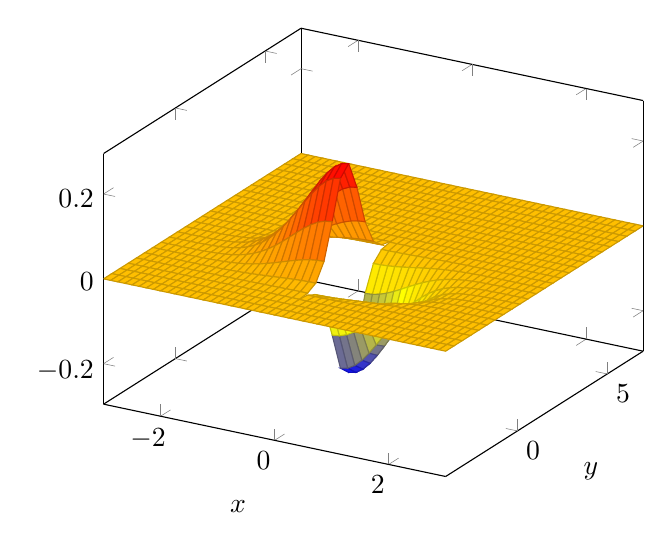
\begin{tikzpicture}
					\begin{axis}[
						view={30}{30},
						xlabel=$x$, ylabel=$y$
					]
					\addplot3[surf, domain =3:0, domain y=-4:7] {-1/4*exp(-x^2-y^2)};
					\addplot3[surf, domain =-3:0, domain y=-4:7] {1/4*exp(-x^2-y^2)};
					\end{axis}
				\end{tikzpicture}
			}
		\end{subfigure}
		\begin{subfigure}{.49\textwidth}
			\centering
			\resizebox{\linewidth}{!}{
				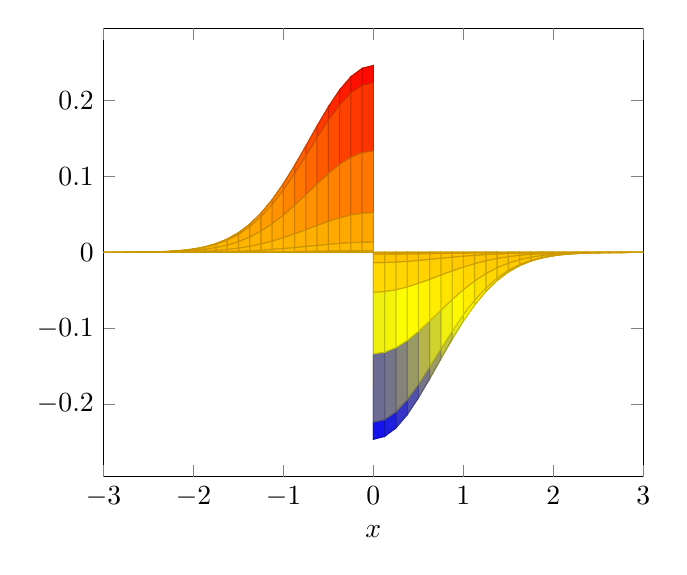
\begin{tikzpicture}
					\begin{axis}[
						view={0}{0},
						xlabel=$x$, ylabel=$y$
					]
					\addplot3[surf, domain =3:0, domain y=-4:7] {-1/4*exp(-x^2-y^2)};
					\addplot3[surf, domain =-3:0, domain y=-4:7] {1/4*exp(-x^2-y^2)};
					\end{axis}
				\end{tikzpicture}
			}
		\end{subfigure}
	\end{figure}
\end{example}
\begin{exercise}
	Sia $f:\R^2 \mapsto \R^m$ derivabile in $x_0$, con $x_0 \in \R^2$. Sia $g:\R^2 \mapsto \R^m$ definita da $g(x,y) = f(y,x)$\\
	Come sono legate le derivate parziali di $f$ e $g$ in $x_0$?
	% TODO solution
\end{exercise}
\begin{exercise}
	Sia $f:A \mapsto \R$ con $A \subseteq \R^n$, derivabile in $x_0 \in \circdot{A}$ . Determinare le derivate parziali in $x_0$ delle funzioni
	\begin{itemize}
		\item $F:A \mapsto \R^2$ definita da $\bigl( f(x), f(x) \bigr)$
		\item $G:A \times A \mapsto \R$ definita da $G(x,y) = f(x) + f(y)$
	\end{itemize}
	% TODO solution
\end{exercise}
\begin{proposition}
	Siano $A \subseteq \R^n$ e $x_0 \in \circdot{A}$. $f$ è \textbf{derivabile parzialmente} rispetto alla $i$-esima coordinata se e solo \textbf{se esiste} finito il limite
	\begin{equation}
		\label{eq:deriv_i_esima}
		\lim\limits_{t \to 0} \frac{f(x_1,\;\dotsc\;,x_i+t,\;\dotsc\;,x_n) - f(x_1,\;\dotsc\;,x_i,\;\dotsc\;,x_n)}{t}
	\end{equation}
	\begin{proof}
		Da \fullref{def:deriv_direz}, sceglendo $v = e_i$ della base canonica si ottiene la \cref{eq:deriv_i_esima}
	\end{proof}
\end{proposition}
\begin{exercise}
	\label{ex:funz_derivabili}
	Formulare in modo rigoroso e dimostrare:
	\begin{enumerate}
		\item La somma di funzioni parzialmente derivabili è parzialmente derivabile.
		\item La composizione di funzioni parzialmente derivabili è parzialmente derivabile.
		\item Prodotto e rapporto, quando definiti, di funzioni parzialmente derivabili sono funzioni parzialmente derivabili.
	\end{enumerate}
	% TODO solution
\end{exercise}
\begin{example}
	Sia $f: \R^2 \mapsto \R^3$ data da
	\begin{equation*}
		f(x,y) =
		\begin{bmatrix}
			2x + 3y\\
			\sin (xy^2)\\
			e^{xy}
		\end{bmatrix}
	\end{equation*}
	La funzione $f$ è derivabile parzialmente su tutto $\R^2$. Inoltre
	\[
		\frac{\partial f}{\partial x}(x,y) =
		\begin{bmatrix}
			2\\
			y^2 \cos (xy^2)\\
			y e^{xy}
		\end{bmatrix}
		\qquad\qquad
		\frac{\partial f}{\partial y}(x,y) =
		\begin{bmatrix}
			3\\
			2xy \cos (xy^2)\\
			x e^{xy}
		\end{bmatrix}
	\]
\end{example}

\begin{proposition}
	Siano $A \subseteq \R^n$, $x_0 \in \circdot{A}$ e $v \in \R^n$ con $v \neq 0$. Sia $f: A \mapsto \R^m$, allora
	\begin{equation*}
		\begin{gathered}
			f \text{ è \textbf{Derivabile} in $x_0$ nella direzione $v$}\\
			\iff\\
			\forall i = 1,\;\dotsc\;,m \quad \text{la \textbf{componente} $f_i$ \textbf{è derivabile} in $x_0$ nella direzione $v$}
		\end{gathered}
	\end{equation*}
	\begin{proof}
		Applicando \fullref{prop:succ_conv_se_comp_conv} e \fullref{prop:cont_e_cont_per_succ} % TODO proper proof. This does not make sense as of now, I know.
	\end{proof}
\end{proposition}
\begin{exercise}
	\label{ex:deriv_non_impl_cont}
	La derivabilità in ogni direzione non implica la continuità. Verificare che la funzione
	\[\funcdef{f}{\R^2}{\R}{(x,y)}
	{
		\begin{cases}
			1 \qquad \text{se } y = x^2 \text{ e } x \neq 0\\
			0 \qquad \text{altrimenti}
		\end{cases}
	}\]
	ammette nell'origine derivate direzionali in ogni direzione ma che \textit{non} è continua nell'origine.
	\begin{figure}[H]
		\begin{subfigure}{.49\textwidth}
			\centering
			\resizebox{\linewidth}{!}{
				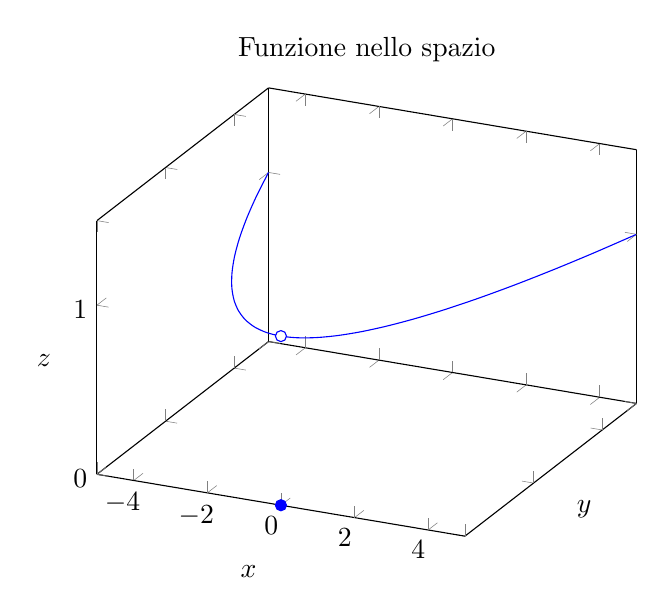
\begin{tikzpicture}
					\begin{axis}[
						title={Funzione nello spazio},
						xlabel=$x$, ylabel=$y$, zlabel=$z$, zlabel style={rotate=-90},
						yticklabels={,,},
						samples y=0,
						zmin = 0, zmax = 1.5
					]
					\addplot3 [smooth, color=blue] (x,x^2,1);
					\addplot3 [color=blue, fill=white, only marks,mark=*] coordinates{(0,0,1)};
					\addplot3 [color=blue, only marks, mark=*] coordinates{(0,0,0)};
					\end{axis}
				\end{tikzpicture}
			}
		\end{subfigure}
		\begin{subfigure}{.49\textwidth}
			\centering
			\resizebox{\linewidth}{!}{
				\begin{tikzpicture}
					\node at (3.4, .2) {$0$};

					\node at (2.1, 1.1) {$1$};
					\node at (4.8, 1.1) {$1$};
					\node at (1.2, 2.5) {$1$};
					\node at (5.65, 2.5) {$1$};
					\node at (.4, 4.5) {$1$};
					\node at (6.5, 4.5) {$1$};

					\node at (1.7, .2) {$0$};
					\node at (6, .6) {$0$};
					\node at (2.6, 2.2) {$0$};
					\node at (5, 3) {$0$};
					\node at (3.2, 4.3) {$0$};
					\node at (1.8, 5) {$0$};
					\begin{axis} [
						title={Valori della $z$},
						axis lines = center,
						xlabel=$x$, ylabel=$y$,
						xticklabels={,,}, yticklabels={,,},
						ymin = -1
					]
						\addplot[color=blue!70, smooth] {x^2};
					\end{axis}
				\end{tikzpicture}
			}
		\end{subfigure}
	\end{figure}

	\begin{solution}
		Le derivate direzionali sono
		\begin{align*}
			\partial_x f(0,0) &= \lim\limits_{t \to 0} \frac{f(0+t,0)-f(0,0)}{t} = 0\\
			\partial_y f(0,0) &= \lim\limits_{t \to 0} \frac{f(0,0+t)-f(0,0)}{t} = 0\\
			D_v f(0,0) &= \lim\limits_{t \to 0} \frac{f(0+t_1,0+t_2)-f(0,0)}{t} = 0
		\end{align*}
		Dunque, per ogni derivata parziale o direzionale in $(0,0)$ il valore della derivata sarà $0$.\\
		D'altro canto $f$ in $0$ \textit{non} è continua in $(0,0)$, quindi si è verificato che la derivabilità non implichi la continuità con $\dim A > 1$
	\end{solution}
\end{exercise}
\begin{exercise}
	Esibire una funzione $f: \R^2 \mapsto \R$ che ammetta in (almeno) un punto una derivata parziale rispetto ad $x$ ma non rispetto a $y$
	\begin{solution}
		La
		\[\funcdef{f}{\R^2}{\R}{(x,y)}{x+\sqrt{y}}\]
		È derivabile parzialmente rispetto a $x$ ma non rispetto a $y$ in $(0,0)$, infatti
		\begin{align*}
			\partial_x f(0,0) &= \lim\limits_{t \to 0} \frac{f(0+t,0)-f(0,0)}{t} = \frac{t-0}{t} = 1\\
			\partial_y f(0,0) &= \lim\limits_{t \to 0} \frac{f(0,0+t)-f(0,0)}{t} = \frac{\sqrt{t}-0}{t} = +\infty \implies \nexists \text{ limite finto}
		\end{align*}
	\end{solution}
\end{exercise}

\section{Derivata Totale}
\begin{definition}[o piccolo]
	\label{def:o_piccolo}
	Siano $A \subseteq \R^n$ e $x_0 \in \circdot{A}$. Siano $f,g: A \mapsto \R^m$ due funzioni.
	\[f=o(g) \text{ per } x \to x_0 \qquad \bydef \lim\limits_{x \to x_0} \frac{\norm{f(x)}}{\norm{g(x)}}\]
	che si legge $f$ è \textbf{o piccolo} di $g$.
	\begin{note}
		Scrivere $f(x) = o(x^k)$ per $x \to 0$ significa che $f = o(g)$ con $g = x^k$
	\end{note}
	\begin{note}
		Con $o(1)$ per $x \to x_0$ si intende una qualunque funzione tendente a $0$ per $x \to x_0$.
	\end{note}
\end{definition}
\begin{exercise}
	Perché son state utilizzate le norme nella \fullref{def:o_piccolo}?
	\begin{solution}
		Perché l'operazione di divisione è sensata solo tra due scalari, non tra vettori.
	\end{solution}
\end{exercise}
\begin{exercise}
	Quali tra le seguenti uguaglianze sono vere? (In tutte, $x \to 0$)
	\begin{itemize}
		\begin{minipage}{0.33\linewidth}
			\item $o(x) = o(x) + o(x)$
			\item $o(x^2) = o(x) \cdot o(x)$
			\item $o(x^2) = o(x) - o(x)$
		\end{minipage}
		\begin{minipage}{0.33\linewidth}
			\item $\sqrt{x} = o(x)$
			\item $o(x) = \abs{o(x)}$
			\item $x = o(\sqrt{x})$
		\end{minipage}
		\begin{minipage}{0.33\linewidth}
			\item $o(x) = 10^6 o(x)$
			\item $x + x^2 = o(x)$
			\item $x = o(x + x^2)$
		\end{minipage}
	\end{itemize}
\end{exercise}
La seguente definizione è da ritenersi già nota da Analisi 1
\begin{definition}[Derivata in $\R$]
	Siano $A \subseteq \R$ e $x_0 \in \circdot{A}$. Sia $f: A \mapsto \R$
	\[f \text{ \textbf{Derivabile} in } x_0 \quad \bydef \quad \lim\limits_{h \to 0} \frac{f(x_0 + h) - f(x_0)}{h} \text{  esiste finito}\]
\end{definition}

Direttamente dalla nozione di Analisi 1 di derivata, si ottiene la seguente relazione tra derivata e coefficiente angolare della retta tangente in un punto
\begin{proposition}[Derivata Analisi 1]
	\label{prop:deriv_analisi_1}
	Siano $A \subseteq \R$ e $x_0 \in \circdot{A}$. Sia $f: A \mapsto \R$
	\begin{equation*}
		\begin{gathered}
			f \text{ è derivabile in } x_0\\
			\iff\\
			\exists m \in \R:\; f(x_0+h) = f(x_0) + mh +o(h) \text{ per } h \to 0
		\end{gathered}
	\end{equation*}
	\begin{proof}
		\begin{align*}
			& f \text{ è derivabile in } x_0\\
			\iff & \lim\limits_{h \to 0} \frac{f(x_0 + h) - f(x_0)}{h} \text{  esiste finito}\\
			\iff & \exists m \in \R:\; \lim\limits_{h \to 0} \frac{f(x_0 + h) - f(x_0)}{h} = m\\
			\iff & \exists m \in \R:\; \lim\limits_{h \to 0} \frac{f(x_0 + h) - f(x_0)}{h} - m = 0\\
			\iff & \exists m \in \R:\; \lim\limits_{h \to 0} \frac{f(x_0 + h) - f(x_0) -mh}{h} = 0
			\shortintertext{Per la nota alla \fullref{def:o_piccolo}}
			\iff & \exists m \in \R:\; f(x_0 + h) - f(x_0) -mh = o(h) \text{ per } h \to 0\\
			\iff & \exists m \in \R:\; f(x_0 + h) = f(x_0) -mh + o(h) \text{ per } h \to 0
		\end{align*}
	\end{proof}
\end{proposition}

\noindent Analogamente a quanto fatto nella \fullref{prop:deriv_analisi_1}, si definisce
\begin{definition}[Differenziale]
	\label{def:differenz}
	Siano $A \subseteq \R^n$ e $x_0 \in \circdot{A}$. Sia $f: A \mapsto \R^m$
	\begin{equation*}
		\begin{gathered}
			f \text{ è \textbf{Differenziabile} in } x_0\\
			\bydef\\
			\exists M \in \mat (m \times n):\; f(x_0 + h) = f(x_0) + Mh + o(h) \text{ per } h \to 0
		\end{gathered}
	\end{equation*}
	La matrice $M$ è la \textbf{Derivata Totale} di $f$ calcolata in $x_0$ e si indica con $Df(x_0)$. $Df(x_0)$ è l'applicazione \textit{lineare} che meglio approssima la variazione di $f$ nelle vicinanze di $x_0$.
\end{definition}
\begin{observation}[Matrici Derivata Totale Particolari]
	\label{obs:matr_deriv_tot}
	Data la matrice $Df(x_0)$ con $m$ righe e $n$ colonne:
	\begin{itemize}
		\item Se $n = 1$ e $m = 1$ $Df(x_0)$ è \textbf{Derivata} di Analisi 1, uno scalare
		\item Se $n > 1$ e $m = 1$ $Df(x_0)$ è \textbf{Gradiente} di $f$ e si indica con $\nabla f(x_0)$ (\textit{nabla} $f$) o $\grad f(x_0)$
		\item Se $n = 1$ e $m > 1$ $Df(x_0)$ è \textbf{Vettore Tangente} alla $f$
		\item Se $n > 1$ e $m > 1$ $Df(x_0)$ è \textbf{Matrice Jacobiana} di $f$ e si può anche indicare con $J_f(x_0)$
	\end{itemize}
	Come si vedrà in \fullref{coro:se_diff_deriv_parz}, il Gradiente della \textit{i-esima} variabile è la \textit{i-esima} colonna di $Df(x_0)$.\\
	Il Vettore Tangente della \textit{j-esima} variabile è invece la \textit{j-esima} riga di $Df(x_0)$.
\end{observation}
\begin{example}
	Esempi relazioni tra Derivata Totale e derivate parziali
	\begin{align*}
		n = 2 \quad m = 1 \qquad & Df =
		\begin{bmatrix}
			\frac{\partial f}{\partial x} & \frac{\partial f}{\partial y}
		\end{bmatrix}\\
		n = 3 \quad m = 1 \qquad & Df =
		\begin{bmatrix}
			\frac{\partial f}{\partial x} & \frac{\partial f}{\partial y} &  \frac{\partial f}{\partial z}
		\end{bmatrix}\\
		n = 1 \quad m = 2 \qquad & Df =
		\begin{bmatrix}
			\frac{\partial f_1}{\partial x}\\[1ex]
			\frac{\partial f_2}{\partial x}
		\end{bmatrix}\\
		n = 2 \quad m = 2 \qquad & Df =
		\begin{bmatrix}
			\frac{\partial f_1}{\partial x} & \frac{\partial f_1}{\partial y}\\[1ex]
			\frac{\partial f_2}{\partial x} & \frac{\partial f_2}{\partial y}
		\end{bmatrix}\\
		n > 2 \quad m > 2 \qquad & Df =
		\begin{bmatrix}
			\frac{\partial f_1}{\partial x_1} & \frac{\partial f_1}{\partial x_2} & \dots & \frac{\partial f_1}{\partial x_n}\\[1ex]
			\frac{\partial f_2}{\partial x_1} & \frac{\partial f_2}{\partial x_2} & \dots & \frac{\partial f_2}{\partial x_n}\\[1ex]
			\vdots & \vdots & \ddots & \vdots\\[1ex]
			\frac{\partial f_m}{\partial x_1} & \frac{\partial f_m}{\partial x_2} & \dots & \frac{\partial f_m}{\partial x_n}
		\end{bmatrix}\\
	\end{align*}
\end{example}
\begin{exercise}
	Perché non è stata data una definizione di derivata attraverso il limite del rapporto incrementale?
	% TODO solution
\end{exercise}
\begin{example}
	Siano $M \in \mat(m \times n)$ una matrice fissata, $f: \R^n \mapsto \R^m$ data da $f(x) = Mx$.\\
	Allora $f$ è differenziabile ovunqe e per ogni $x_0 \in \R$ si ha $Df(x_0) = M$
\end{example}
\begin{proposition}[Unicità della Derivata Totale]
	\label{prop:unic_deriv_tot}
	Siano $A \subseteq \R^n$, $x_0 \in \circdot{A}$, $f: A \mapsto \R^m$ e $M_1, M_2 \in \mat(m \times n)$
	\begin{equation*}
		\left.
		\begin{array}{l}
			M_1 \text{ derivata totale di } f \text{ in } x_0\\
			M_2 \text{ derivata totale di } f \text{ in } x_0
		\end{array}
		\right\}
		\implies
		M_1 = M_2
	\end{equation*}
	\begin{proof}
		Sia $h \in \R$. Fissato un vettore $e_i$ della base canonica di $\R^n$
		\begin{align*}
			M_2 e_i - M_1 e_1 &=\\
			\shortintertext{Moltiplicando e dividendo per $h$}
			&= \frac{1}{h} M_2 e_i h - \frac{1}{h} M_1 e_i h\\
			&= \frac{1}{h} [M_2 e_i h - M_1 e_i h]
			\shortintertext{Grazie alla \fullref{def:differenz}}
			&= \frac{1}{h} [f(x_0 + h e_i) - f(x_0) + o(h)] - \frac{1}{h} [f(x_0 + h e_i) - f(x_0) + o(h)]\\
			&= o(h) \text{ per } t \to 0
		\end{align*}
		Passando al limite per $t \to 0$, si deduce che le applicazioni lineari $M_1$ e $M_2$ hanno le stesse immagini sui vettori della base canonica, quindi coincidono.
	\end{proof}
\end{proposition}
\begin{proposition}
	Siano $A \subseteq \R^n$, $x_0 \in \circdot{A}$ e $f:A \mapsto \R^m$
	\[f \text{ \textbf{Differenziabile} in } x_0 \implies f \text{ \textbf{Continua} in } x_0\]
	\begin{proof}
		Per ipotesi $x_0 \in \circdot{A}$, dunque $x_0$ è di accumulazione. A questo punto, grazie alla \fullref{prop:f_cont_se_isol_o_accum} basta verificare che $\lim\limits_{x \to x_0} f(x) = f(x_0)$.
		Dalla \fullref{def:differenz}
		\[f(x_0 + h) = f(x_0) + Mh + o(h) \text{ per } h \to 0\]
		Quindi, posto $h = x - x_0$ ed essendo $M = Df(x_0)$ per \fullref{def:differenz}
		\[\lim\limits_{x \to x_0} f(x) = \lim\limits_{x \to x_0} \bigl[f(x_0) + Df(x_0)(x-x_0) + o(x - x_0)\bigr] = f(x_0)\]
	\end{proof}
\end{proposition}
\begin{proposition}
	\label{prop:se_diff_deriv_dir}
	Siano $A \subseteq \R^n$, $x_0 \in \circdot{A}$ e $f:A \mapsto \R^m$
	\[
		f \text{ \textbf{Differenziabile} in } x_0
		\implies
		\begin{cases}
			\begin{array}{c}
				f \text{ ammette ogni \textbf{Derivata Direzionale} in } x_0\\
				e\\
				\forall v \in \R^n \setminus \brackets{0} D_v f(x_0) = Df(x_0)v
			\end{array}
		\end{cases}
	\]
	\begin{proof}
		Sia $v \in \R^n$ non nullo. Partendo dalla \fullref{def:deriv_direz}
		\begin{align*}
			&\lim\limits_{t \to 0} \frac{f(x_0 + tv) - f(x_0)}{t}
			\shortintertext{Sostituendo ora $f(x_0 + tv)$ con il secondo membro della \fullref{def:differenz}, dopo aver posto $h = tv$}
			= &\lim\limits_{t \to 0} \frac{\cancel{f(x_0)} + Df(x_0)(tv) + o(tv) - \cancel{f(x_0)}}{t}\\
			= &\lim\limits_{t \to 0} \frac{Df(x_0)(tv)}{t} + \lim\limits_{t \to 0} \frac{o(tv)}{t}\\
			= &Df(x_0)v
		\end{align*}
	\end{proof}
\end{proposition}
\begin{corollary}
	\label{coro:se_diff_deriv_parz}
	Siano $A \subseteq \R^n$, $x_0 \in \circdot{A}$ e $f:A \mapsto \R^m$
	\[
		f \text{ \textbf{Differenziabile} in } x_0
		\implies
		\begin{cases}
			\begin{array}{c}
				f \text{ ammette ogni \textbf{Derivata Parziale} in } x_0\\
				e\\
				\frac{\partial f}{\partial x_i}(x_0) = Df(x_0) \cdot e_i
			\end{array}
		\end{cases}
	\]
	Dove $Df(x_0) \cdot e_i$ non è altro che
	\[
		Df(x_0) \cdot e_i =
		\begin{bmatrix}
			x_{11} & x_{12} & \dots & x_{1n}\\
			x_{21} & x_{22} & \dots & x_{2n}\\
			\vdots & \ddots & & \vdots\\
			x_{n1} & x_{n2} & \dots & x_{nn}\\
		\end{bmatrix}
		\cdot
		\begin{bmatrix}
			(0 & \dots & 1 & \dots & 0)
		\end{bmatrix}
		=
		\begin{bmatrix}
			0 & \dots & x_{1i} & 0\\
			0 & \dots & x_{2i} & 0\\
			\vdots & \ddots & & \vdots\\
			0 & \dots & x_{ni} & 0\\
		\end{bmatrix}
	\]
	Cioè l'\textit{i-esima} colonna della $Df(x_0)$, come da \fullref{obs:matr_deriv_tot}
	\begin{note}
		Per quanto detto, il presente corollario offre il principale metodo di calcolo della \textbf{Derivata Totale}\\
		Inoltre è anche una dimostrazione alternativa della \fullref{prop:unic_deriv_tot}
	\end{note}
	\begin{proof}
		Direttamente dalla \fullref{prop:se_diff_deriv_dir} e dalla \fullref{def:deriv_direz} (sezione sulle derivate parziali)
	\end{proof}
\end{corollary}
\begin{observation}
	Sia \fullref{prop:se_diff_deriv_dir} che \fullref{coro:se_diff_deriv_parz} non possono essere invertiti, come verificato in \fullref{ex:deriv_non_impl_cont}.
\end{observation}
\begin{corollary}
	Siano $A \subseteq \R^n$, $x_0 \in \circdot{A}$ e $f:A \mapsto \R^m$
	\[f \text{ \textbf{Differenziabile} in } x_0 \implies f \text{ \textbf{Derivabile} in } x_0\]
	\begin{proof}
		Mediante il \fullref{coro:se_diff_deriv_parz} si vede immediatamente che rispetta la \fullref{def:deriv_direz}
	\end{proof}
\end{corollary}
\begin{corollary}
	\label{coro:f_diff_con_matr_comp}
	Siano $A \subseteq \R^n$, $x_0 \in \circdot{A}$ e $f:A \mapsto \R^m$. Sia $f$ derivabile parzialmente in $x_0$ e sia $M$ la $Df(x_0)$, matrice dei coefficienti $M_{ij} = \frac{\partial f_i}{\partial x_j}$
	\begin{equation*}
		\begin{gathered}
			f \text{ \textbf{Differenziabile} in } x_0\\
			\iff\\
			f(x_0 + h) - f(x_0) - Mh = o(h) \text{ per } h \to 0
		\end{gathered}
	\end{equation*}
	\begin{proof}
		Direttamente dalla \fullref{def:differenz}, per mezzo del \fullref{coro:se_diff_deriv_parz}.
	\end{proof}
\end{corollary}
\begin{exercise}
	Verificare che, nel caso $n = 2$ ed $m = 1$ il \fullref{coro:f_diff_con_matr_comp} si scrive
	\begin{equation*}
		\begin{gathered}
			f \text{ \textbf{Differenziabile} in } x_0\\
			\iff\\
			f(x_0 + h, y_o + k) - f(x_0, y_0) -
			\begin{bmatrix}
				\frac{\partial f}{\partial x}(x_0, y_0) & \frac{\partial f}{\partial y}(x_0, y_0)
			\end{bmatrix}
			\cdot
			\begin{bmatrix}
				h\\
				k
			\end{bmatrix}
			= o(\sqrt{h^2 + k^2}) \text{ per } h, k \to 0
		\end{gathered}
	\end{equation*}
	% TODO solution
\end{exercise}
\begin{exercise}
	Scrivere il \fullref{coro:f_diff_con_matr_comp} nel caso $n = 3$ ed $m = 1$
	% TODO solution
\end{exercise}

\begin{theorem}[del Differenziale Totale]
	\label{teo:diff_tot}
	Siano $A \subseteq \R^n$, $x_0 \in \circdot{A}$ e $f:A \mapsto \R^m$.
	\[
		\left.
		\text{
			\begin{tabular}{c}
				Per $i = 1,\;\dotsc\;,m$ e $j = 1,\;\dotsc\;,n$\\
				$\frac{\partial f_i}{\partial x_j}$ è \textbf{definita} in un \textbf{intorno} di $x_0$ e \textbf{Continua} in $x_0$
			\end{tabular}
		}
		\right\}
		\implies\\
		f \text{ è \textbf{Differenziabile} in } x_0
	\]
	\begin{note}
		È specificata la necessità di continuità in un intorno di $x_0$ in quanto, come detto in \fullref{def:deriv_direz}, l'esistenza di derivate parziali non garantisce la continuità.
	\end{note}
	\begin{proof}
		Si può supporre $n = 2$ e $m = 1$ in quanto il caso più generale è del tutto analogo.\\
		È necessario verificare la \fullref{def:differenz}, dunque in $\R^n = \R^2$ si ha
		\begin{equation}
			\label{eq:deriv_tot_def_diff}
			f(x_0 + h, y_0 + k) = f(x_0, y_0) + Df(x_0, y_0) \begin{bmatrix}h\\k\end{bmatrix} + o(h,k) \text{ per } h,k \to 0
		\end{equation}
		Considerando solo i primi due addendi, aggiungendo e sottraendo la stessa quantità, si ottiene
		\begin{equation}
			\label{eq:teo_diff_tot_sommo_sottraggo}
			f(x_0 + h, y_0 + k) - f(x_0, y_0) = \underbrace{f(x_0 + h, y_0 + k) - f(x_0+h,y_0)}_{\text{(1)}} + \underbrace{f(x_0+h,y_0) - f(x_0, y_0)}_{\text{(2)}}
		\end{equation}
		Considerando la (1) e la (2) di \cref{eq:teo_diff_tot_sommo_sottraggo} come funzioni in una sola variabile, si può applicare il Teorema di Lagrange di Analisi 1
		\begin{itemize}
			\item La (1) rispetto a $y$, con $x_0 + h$ fissato
			\item La (2) rispetto a $x$, con $y_0$ fissato
		\end{itemize}
		Spostandosi lungo le direzioni parallele agli assi è possibile andare da $(x_0 + h, y_0 + k)$ a $(x_0, y_0)$
		\begin{center}
			\begin{tikzpicture}
				\pgfmathsetmacro\MAX{8}
				\pgfmathsetmacro\XZ{\MAX / 3 }
				\pgfmathsetmacro\YZ{\MAX / 3 }
				\pgfmathsetmacro\XZh{\MAX / 3 *2}
				\pgfmathsetmacro\YZk{\MAX / 3 *2}
				\coordinate (X0Y0) at (\XZ,\YZ);
				\coordinate (X0hY0) at (\XZh,\YZ);
				\coordinate (X0Y0k) at (\XZ,\YZk);
				\coordinate (X0hY0k) at (\XZh,\YZk);

				\draw[->] (0,0) -- (\MAX,0) node[anchor=north west] {$x$};
				\draw[->] (0,0) -- (0,\MAX) node[anchor=south east] {$y$};
				\draw[dotted] (\XZ,0) -- (\XZ,\MAX);
				\draw[dotted] (0,\YZ) -- (\MAX,\YZ);
				\draw[dotted] (\XZh,0) -- (\XZh,\MAX);
				\draw[dotted] (0,\YZk) -- (\MAX,\YZk);
				\draw node[anchor=north] at (\XZ,0) {$x_0$};
				\draw node[anchor=north] at (\XZh,0) {$x_0+h$};
				\draw node[anchor=east] at (0,\YZ) {$y_0$};
				\draw node[anchor=east] at (0,\YZk) {$y_0+k$};
				\draw node at (X0Y0) {$\bullet$};
				\draw node at (X0Y0k) {$\bullet$};
				\draw node at (X0hY0) {$\bullet$};
				\draw node at (X0hY0k) {$\bullet$};
				\draw node[anchor=north east] at (X0Y0) {$(x_0,y_0)$};
				\draw node[anchor=south east] at (X0Y0k) {$(x_0,y_0+k)$};
				\draw node[anchor=north west] at (X0hY0) {$(x_0+h,y_0)$};
				\draw node[anchor=south west] at (X0hY0k) {$(x_0+h,y_0+k)$};

				\draw[<-] (\XZ,\MAX*4/10) -- (\XZ,\MAX*6/10);
				\draw[<-] (\XZh,\MAX*4/10) -- (\XZh,\MAX*6/10);
				\draw[<-] (\MAX*4/10,\YZ) -- (\MAX*6/10,\YZ);
				\draw[<-] (\MAX*4/10,\YZk) -- (\MAX*6/10,\YZk);
			\end{tikzpicture}
		\end{center}
		Quindi, applicando il teorema di Lagrange (vedere Nota al termine della dimostrazione):
		\[
			\exists \alpha, \beta \in \intervalopen{0}{1} \textbf{ per cui} \qquad
			\begin{array}{rrcl}
				\text{(1)} & f(x_0 + h, y_0 + k) - f(x_0 + h, y_0) &=& \frac{\partial f}{\partial y} (x_0 + h, y_0 + \beta k) k\\[1ex]
				\text{(2)} & f(x_0 + h, y_0) - f(x_0, y_0) &=& \frac{\partial f}{\partial x} (x_0 + \alpha h, y_0) h
			\end{array}
		\]
		Tornando alla \cref{eq:deriv_tot_def_diff}, si ottiene
		\begin{align*}
			&f(x_0 + h, y_0 + k) - f(x_0, y_0) - Df(x_0, y_0) \begin{bmatrix}h\\k\end{bmatrix}\\
			= &\underbrace{f(x_0 + h, y_0 + k) - f(x_0+h,y_0)}_{\text{(1)}} + \underbrace{f(x_0+h,y_0) - f(x_0, y_0)}_{\text{(2)}} - Df(x_0, y_0) \begin{bmatrix}h\\k\end{bmatrix}\\
			= &\underbrace{\frac{\partial f}{\partial y} (x_0 + h, y_0 + \beta k) k}_{\text{(1)}} + \underbrace{\frac{\partial f}{\partial x} (x_0 + \alpha h, y_0) h}_{\text{(2)}} - Df(x_0, y_0) \begin{bmatrix}h\\k\end{bmatrix}
			\shortintertext{Si esegue il prodotto tra matrice Derivata Totale e vettore, infine si separano i termini}
			= &	\left( \frac{\partial f}{\partial y} (x_0 + h, y_0 + \beta k) - \frac{\partial f}{\partial y} (x_0 + h, y_0) \right) k +
				\left( \frac{\partial f}{\partial x} (x_0 + \alpha h, y_0) - \frac{\partial f}{\partial x} (x_0, y_0)\right) h
		\end{align*}
		Si passa dunque alla norma
		\begin{align*}
			&\norm{f(x_0 + h, y_0 + k) - f(x_0, y_0) - Df(x_0, y_0) \begin{bmatrix}h\\k\end{bmatrix}}\\
			\shortintertext{Separando come fatto prima ed applicando la disguguaglianza triangolare}
			\leq &	\norm{\left( \frac{\partial f}{\partial y} (x_0 + h, y_0 + \beta k) - \frac{\partial f}{\partial y} (x_0 + h, y_0) \right) k} +
					\norm{\left( \frac{\partial f}{\partial x} (x_0 + \alpha h, y_0) - \frac{\partial f}{\partial x} (x_0, y_0)\right) h}
			\shortintertext{Per proprietà 4 da \fullref{def:norma}}
			= & \norm{\frac{\partial f}{\partial y} (x_0 + h, y_0 + \beta k) - \frac{\partial f}{\partial y} (x_0 + h, y_0)} \abs{k} +
				\norm{\frac{\partial f}{\partial x} (x_0 + \alpha h, y_0) - \frac{\partial f}{\partial x} (x_0, y_0)} \abs{h}
			\shortintertext{Presa ora la norma del vettore $(h,k)$, cioè $\norm{(h,k)} = \sqrt{h^2 + k^2}$, sicuramente $\abs{h} \leq \norm{(h,k)}$ e $\abs{k} \leq \norm{(h,k)}$, dunque}
			\leq &	\norm{\frac{\partial f}{\partial y} (x_0 + h, y_0 + \beta k) - \frac{\partial f}{\partial y} (x_0 + h, y_0)} \sqrt{h^2 + k^2} +
					\norm{\frac{\partial f}{\partial x} (x_0 + \alpha h, y_0) - \frac{\partial f}{\partial x} (x_0, y_0)} \sqrt{h^2 + k^2}
			\shortintertext{Essendo $h,k \to 0$ da \cref{eq:deriv_tot_def_diff} e graze alla continuità delle derivate, le due norme tendono a $0$. Inoltre, per \fullref{def:o_piccolo}}
			=\; &o(1) \sqrt{h^2 + k^2} \text{ per } \begin{bmatrix}h\\k\end{bmatrix} \to 0\\
			=\; &o(\sqrt{h^2 + k^2}) \text{ per } \begin{bmatrix}h\\k\end{bmatrix} \to 0
		\end{align*}
		Da cui la tesi, avendo verificato la \fullref{def:differenz}.
		\begin{note}
			Il \textbf{Teorema di Lagrange} (o del \textbf{Valor Medio Differenziale})
			\[c \in \intervalopen{a}{b} : f'(c) = \frac{f(b)-f(a)}{b - a}\]
			Alternativamente, nella forma
			\[\xi \in \intervalopen{0}{1} : f'(x_0 + \xi h) = \frac{f(x_0 + h)-f(x_0)}{h}\]
		\end{note}
	\end{proof}
\end{theorem}
\begin{exercise}
	Data la funzione
	\[
		\funcdef{f}{\R}{\R}{x}{
			\begin{cases}
				\begin{array}{ll}
					x^2 \sin \frac{1}{x} & x \neq 0\\
					0 & x = 0
				\end{array}
			\end{cases}
		}
	\]
	Verificare che $f$ è differenziabile su $\R$ ma non ha derivata continua su $\R$.
	% TODO solution
\end{exercise}

\begin{definition}[Funzioni di Classe $\cntclass{1}$]
	Sia $A \subseteq \R^n$ un \textbf{Aperto}.
	\begin{center}
		$\cntclass{1}(A; \R^m)$ è l'insieme delle funzioni $f:A \mapsto \R^m$\\
		con \textbf{tutte} le \textbf{Derivate Parziali prime} in ogni punto di $A$
	\end{center}
	Si può anche leggere \textit{$f$ è di classe $\cntclass{1}$ su $A$ con valori in $\R^m$}.
\end{definition}
\begin{corollary}
	Sia $A \subseteq \R^n$ un \textbf{Aperto}. Se $f \in \cntclass{1}(A;\R^m)$ allora $f$ è \textbf{Differenziabile} su $A$.
	\begin{proof}
		Applicare la \fullref{teo:diff_tot}
	\end{proof}
\end{corollary}
\begin{proposition}
	\label{prop:cnt_class_components}
	Siano $m \in \N, m \geq 1$ e $A \subseteq \R^n$ un \textbf{Aperto}
	\[f \in \cntclass{1}(A; \R^m) \iff \forall i = 1,\;\dotsc\;, m \quad f_i \in \cntclass{1}(A;\R)\]
	\begin{proof}
		Immediata.
	\end{proof}
\end{proposition}
\begin{exercise}
	Dimostrare la \fullref{prop:cnt_class_components}.
	% TODO solution
\end{exercise}
\begin{exercise}
	Dimostrare che $\cntclass{1}(A;\R)$ non coincide con l'insieme delle funzioni differenziabili su $A$ con valori in $\R$.
	% TODO solution
\end{exercise}
\begin{proposition}
	\label{prop:if_df_lim_then_unif_cont}
	Siano $I \in \R$ un intervallo reale e $f(x)$ una funzione \textbf{Derivabile} in $I$. Se la $f'(x)$ è una \textbf{Funzione Limitata} in $I$, allora f è \textbf{Uniformemente Continua} in $I$ % Taken from http://www.batmath.it/matematica/an_uno/cont_unif/cont_unif.htm
	\begin{proof}
		Omessa. % TODO proof
	\end{proof}
\end{proposition}

\subsection{Regole di Derivazione}
%TODO This section is a placeholder, the following proposition have to be rewritten
\proposition
Siano $f,g: A\subseteq \R^n \rightarrow \R^m$ e $x_0\in\circdot{A}$\\
$f$ differenziabile in $x_0$, $g$ differenziabile in $x_0$ allora $f+g$ differenziabile in $x_0$ e $D(f+g)(x_0) = Df(x_0)+Dg(x_0)$
\begin{proof}
	$f$ è differenziabile, allora $f(x_0+h)=f(x_0)+Df(x_0)h+o(h)$ per $h\rightarrow 0$\\
	anche $g$ lo è, quindi $g(x_0+h)=g(x_0)+Dg(x_0)h+o(h)$ per $h\rightarrow 0$\\
	sommando membro a membro si ottiene  $(f+g)(x_0+h)=(f+g)(x_0)+[Df(x_0)+Dg(x_0)]h+o(h)$ per $h\rightarrow 0$\\
	Questa è la definizione di differenziabilità, allora $f+g$ è differenziabile e $D(f+g)(x_0) = Df(x_0)+Dg(x_0)$
\end{proof}

\proposition
Sia $f: A\subseteq \R^n \rightarrow \R^m$ e $x_0\in\circdot{A}$ e $\lambda\in \R$\\
$f$ differenziabile in $x_0$ allora $\lambda f$ differenziabile in $x_0$ e $D(\lambda f)(x_0) = \lambda Df(x_0)$
\begin{proof}
	$f$ è differenziabile, allora $f(x_0+h)=f(x_0)+Df(x_0)h+o(h)$ per $h\rightarrow 0$\\
	valuto ora $(\lambda f)(x_0+h)=(\lambda f)(x_0)+\lambda Df(x_0)h+o(h)$ per $h\rightarrow 0$\\
	Questa è la definizione di differenziabilità, allora $\lambda f$ è differenziabile e $D(\lambda f)(x_0) = \lambda Df(x_0)$
\end{proof}

\proposition
Sia $g: A\subseteq \R^n \rightarrow \R^m$ e $x_0\in\circdot{A}$\\
Sia $f: B\subseteq \R^m \rightarrow \R^p$ e $g(x_0)\in\circdot{B}$\\
$f$ differenziabile in $g(x_0)$, $g$ differenziabile in $x_0$ allora $f\circ g$ differenziabile in $x_0$ e $D(f\circ g)(x_0) = Df(g(x_0))*Dg(x_0)$
\begin{proof}
	$g$ è differenziabile in $x_0$, allora $g(x_0+h)=f(x_0)+Dg(x_0)h+o(h)$ per $h\rightarrow 0$\\
	$f$ è differenziabile in $g(x_0)$ allora $g(g(x_0)+k)=f(g(x_0))+Df(g(x_0))k+o(k)$ per $k\rightarrow 0$\\
	valuto ora 
	\[(f\circ g)(x_0+h) = f(g(x_0+h)+Dg(x_0)h+o(h)) = \] 
	\[=f(g(x_0))+Df(g(x_0))(Dg(x_0)h+o(h))+o(Dg(x_0)h+o(h)) = \]
	\[=(f\circ g)(x_0) + Df(g(x_0))Dg(x_0)h+Df(g(x_0))o(h)+Dg(x_0)o(h)+o(h)\]
	
	con $h$ un vettore $n\times 1$\\
	con $Dg$ una matrice $m\times n$\\
	con $Df$ una matrice $p\times m$\\
	
	da rivedere un pochino ....
	
	Questa è la definizione di differenziabilità, allora $f\circ g$ è differenziabile e $D(f\circ g)(x_0) = Df(g(x_0))Dg(x_0)$
\end{proof}
\proposition DERIVATA DEL PRODOTTO

\subsection{La Formula degli Accrescimenti Finiti}
\begin{definition}[Segmento]
	\label{def:segmento}
	Siano $x_0,x_1 \in \R^n$, si dice \textbf{Segmento} di estremi $x_0$ e $x_1$ l'insieme che li unisce, cioè
	\[S = \brackets{tx_1+(1-t)x_0 \in \R^n:\; t \in \intervalclose{0}{1}}\]
\end{definition}
\begin{observation}
	La \fullref{def:segmento} può essere formulata in ogni spazio affine o vettoriale
\end{observation}
\begin{exercise}
	Dimostrare che ogni \textbf{Segmento} in $\R^n$ è \textbf{Compatto} e \textbf{Connesso}.
	\begin{solution}
		Posta
		\[\funcdef{\varphi}{\intervalclose{0}{1}}{\R^n}{t}{t x_1 + (1-t) x_0}\]
		\begin{itemize}
			\item $\intervalclose{0}{1} \subset \R^n$, essendo sottoinsieme di $\R^n$ chiuso e limitato, grazie alla \fullref{prop:compat_chius_lim_Rn}, è compatto. Inoltre, grazie al \fullref{teo:weier_generale}, $\varphi(\intervalclose{0}{1})$ è sicuramente compatto a sua volta, dunque il segmento $S$ è compatto.
			\item Dalla \fullref{prop:f_di_conn_cont_e_conn}, essendo $\varphi$ continua, il segmento $S$ è sicuramente Connesso.
		\end{itemize}
	\end{solution}
\end{exercise}
\begin{exercise}
	Ispirandosi alla \fullref{def:segmento} è possibile dare una possibile definizione di Semiretta uscente da $x_0$ e passante per $x_1$?
	\begin{solution}
		\[s = \brackets{x_0+(x_1-x_0)t \in \R^n: t \in \intervalclop{0}{+\infty} \;}\]
	\end{solution}
\end{exercise}
\begin{theorem}[degli Accrescimenti Finiti]
	\label{teo:accresc_fin}
	Sia $f \in \cntclass{1}(A;\R^m)$, con $A \subseteq \R^n$. Siano $x_0, x_1 \in \circdot{A}$ tali che il \textbf{Segmento} $S$ di estremi $x_0$ e $x_1$ sia \textbf{interamente contenuto} in $\circdot{A}$. Allora
	\begin{equation}
		\label{eq:accresc_fin}
		\norm{f(x_1) - f(x_0)} \leq \sup\limits_{\xi \in S} \norm{Df(\xi)} \cdot \norm{x_1-x_0}
	\end{equation}
	\begin{note}
		Con $\R^m = \R^1$ e $A \subseteq \R^1$ è come dire
		\[
			\abs{f(x_1) - f(x_0)} \leq M \cdot \abs{x_1 - x_0} \quad \text{con} \quad M = \sup \brackets{\text{\itshape\begin{tabular}{c}coefficiente angolare di tutte le\\rette tangenti alla curva\end{tabular}}}
		\]
		\begin{center}
			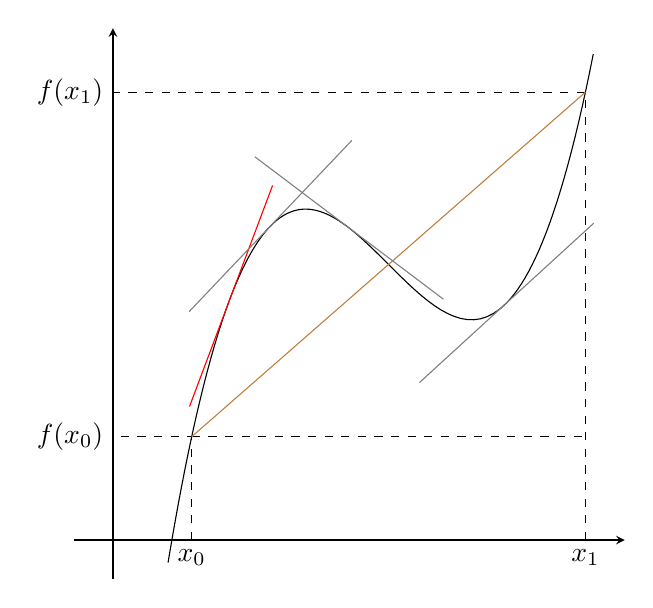
\begin{tikzpicture}[declare function = {curve(\x)=0.3*(\x-3.5)^3-\x+7; x_0=1; x_1=6;}]
				% Axes
				\draw[-stealth] (-0.5,0) -- (6.5,0);
				\draw[-stealth] (0,-0.5) -- (0,6.5);
				% Curve
				\draw[domain=.7:1.5] plot (\x,{curve(\x)}) {[turn] (-1.5,0) coordinate(t0) (1.5,0) coordinate(t1)}; % This is the most steep tangent
				\draw[domain=1.5:2] plot (\x,{curve(\x)}) {[turn] (-1.5,0) coordinate(t2) (1.5,0) coordinate(t3)};
				\draw[domain=2:3] plot (\x,{curve(\x)}) {[turn] (-1.5,0) coordinate(t4) (1.5,0) coordinate(t5)};
				\draw[domain=3:5] plot (\x,{curve(\x)}) {[turn] (-1.5,0) coordinate(t6) (1.5,0) coordinate(t7)};
				\draw[domain=5:6.1] plot (\x,{curve(\x)});
				% Dashed lines
				\foreach \x in {x_0,x_1}
				{\draw[dashed] (\x,0) node[below]{$\x$} |- (0,{curve(\x)}) node[left] {$f(\x)$};}
				\draw[dashed] (x_0,{curve(x_0)}) -- (x_1,{curve(x_0)});
				% Delta-y
				\draw[brown] ({x_0},{curve(x_0)}) -- ({x_1},{curve(x_1)});
				% Tangents
				\draw[red] (t0)--(t1);
				\draw[black!50] (t2)--(t3);
				\draw[black!50] (t4)--(t5);
				\draw[black!50] (t6)--(t7);
			\end{tikzpicture}
		\end{center}
	\end{note}
	\begin{proof}
		Si può dare per scontato che $x_1 \neq x_0$, in quanto, se $x_1 = x_0$ , allora $f(x_1) = f(x_0)$ e la \cref{eq:accresc_fin} diventerebbe $0 \leq 0$. La tesi sarebbe quindi verificata direttamente.\\
		Fissato un qualsiasi $v \in \R^m$, si definisce così la funzione $F$ legata ad $f$ tramite la \fullref{def:segmento}:
		\begin{equation}
			\label{eq:accresc_fin_F}
			\funcdef{F}{\intervalclose{0}{1}}{\R}{t}{v \cdot f \bigl( t x_1 + (1-t)x_0 \bigr)}
		\end{equation}
		\begin{note}
			Nella \cref{eq:accresc_fin_F},  $\cdot$  è Prodotto Scalare tra due vettori di dimensione $\R^m$, dunque il risultato è correttamente uno scalare.
		\end{note}
		$F$ è continua e derivabile sull'intervallo di definizione $\intervalclose{0}{1}$. È dunque possibile utilizzare il Teorema di Lagrange da Analisi 1, che garantisce:
		\[\exists c \in \intervalopen{0}{1}: \quad F(1) - F(0) = F'(c) \; (1-0)\]
		Tornando dunque a $f$ dalla definizione di $F$
		\[v \cdot f(x_1) - v \cdot f(x_0) = v \cdot Df\bigl( cx_1 + (1-c)x_0 \bigr) (x_1 - x_0)\]
		Ricordando che la $F$ è a valori in $\R$, si può calcolare il valore assoluto mantenendo l'uguaglianza
		\[\abs{v \cdot f(x_1) - v \cdot f(x_0)} = \abs{v \cdot Df\bigl( cx_1 + (1-c)x_0 \bigr) (x_1 - x_0)}\]
		Essendo il secondo membro il valore assoluto di un prodotto scalare, si può applicare ad esso la \textbf{Disuguaglianza di Cauchy-Schwarz} ed ottenere
		\[\abs{v \cdot \bigl( f(x_1) - f(x_0) \bigr)} \leq \norm{v} \cdot \norm{Df\bigl( cx_1 + (1-c)x_0 \bigr) (x_1 - x_0)}\]
		Dunque, seaparando ulteriorimente le norme si arriva alla:
		\begin{equation}
			\label{eq:accr_fin_norm}
			\abs{v \cdot \bigl( f(x_1) - f(x_0) \bigr)} \leq \norm{v} \cdot \norm{Df\bigl( cx_1 + (1-c)x_0 \bigr)} \cdot \norm{x_1 - x_0}
		\end{equation}

		Essendo, come detto all'inzio, $f(x_1) \neq f(x_0)$ è ora possibile scegliere un $v$ "comodo", come:
		\[v = \frac{1}{\norm{f(x_1) - f(x_0)}} \cdot \bigl( f(x_1) - f(x_0) \bigr)\]
		\begin{note}
			La norma di $v$, grazie poi alla proprietà 4 da \fullref{def:norma}, è
			\begin{align*}
				\norm{v} &= \norm{
					\underbrace{\frac{1}{\norm{f(x_1) - f(x_0)}}}_{\text{Scalare}}
					\cdot
					\underbrace{\bigl( f(x_1) - f(x_0) \bigr)}_{\text{Vettore}}
					}\\
				&= \abs{\frac{1}{\norm{f(x_1) - f(x_0)}}} \cdot \norm{\bigl( f(x_1) - f(x_0) \bigr)}\\
				&= \frac{1}{\norm{f(x_1) - f(x_0)}} \cdot \norm{\bigl( f(x_1) - f(x_0) \bigr)}\\
				&= 1
			\end{align*}
		\end{note}
		Sostituendo dunque in \cref{eq:accr_fin_norm} si ottiene
		\[\norm{\frac{1}{\norm{f(x_1) - f(x_0)}} \cdot \bigl( f(x_1) - f(x_0) \bigr) \cdot \bigl( f(x_1) - f(x_0) \bigr)} \leq \cdot \norm{Df\bigl( cx_1 + (1-c)x_0 \bigr)} \cdot \norm{x_1 - x_0}\]
		Dal punto 3 di \fullref{ex:sp_norm}, si ottiene
		\[\norm{\frac{1}{\norm{f(x_1) - f(x_0)}} \cdot \norm{f(x_1) - f(x_0)}^2} \leq \norm{Df\bigl( cx_1 + (1-c)x_0 \bigr)} \cdot \norm{x_1 - x_0}\]
		Da cui
		\[\norm{f(x_1) - f(x_0)} \leq \norm{Df\bigl( cx_1 + (1-c)x_0 \bigr)} \cdot \norm{x_1 - x_0}\]
		e passando al $\sup$ su $t \in \intervalopen{0}{1}$ si ottiene la tesi.
	\end{proof}
\end{theorem}
Il seguente esercizio mostra come il Teorema di Lagrange di Analisi 1 non possa essere esteso al caso di funzioni a valori in $\R^n$ con $n > 1$.
\begin{exercise}
	Sia $f: \R \mapsto \R^2$ data da $f(t) = (\cos t, \sin t)$. Mostrare che non esiste nessun numero reale $c$ tale che
	\[f(2 \pi) - f(0) = Df(c) \cdot 2 \pi\]
\end{exercise}

\begin{definition}[Insieme Convesso]
	\label{def:convesso}
	Sia $C \subseteq \R^n$
	\begin{equation*}
		\begin{gathered}
			C \text{ è \textbf{Convesso}}\\
			\bydef\\
			\forall x_0,y_1 \in C \quad \brackets{tx_1+(1-t)x_0:\; t \in \intervalclose{0}{1}} \subseteq C
		\end{gathered}
	\end{equation*}
	Cioè un insieme è Convesso se, dati qualsiasi due suoi punti, contiene anche il segmento che li congiunge.
\end{definition}
\begin{exercise}
	Dimostrare la \fullref{prop:convesso_deriv_par_lim_allora_lips}
	% TODO solution
\end{exercise}
\begin{exercise}
	In $\R^n$ dimostrare che ogni segmento è convesso, così come anche ogni sfera.\\
	Esibire un esempio di insieme non convesso.
	% TODO solution
\end{exercise}
\begin{corollary}
	\label{coro:convess_nabla_0_f_const}
	Siano $A \subseteq \R^n$ e $f: A \mapsto \R$
	\[
		\left.
			\begin{array}{l}
				A \text{ \textbf{Aperto Convesso}}\\
				f \text{ \textbf{Differenziabile} in } A\\
				\forall x \in A \quad \nabla f(x) = 0
			\end{array}
		\right\}
		\implies\\
		f \text{ è \textbf{Costante} su } A
	\]
	\begin{note}
		Come da \fullref{obs:matr_deriv_tot}, $\nabla f(x) = Df(x) \in \mat (1 \times n)$, cioè un vettore riga.
	\end{note}
	\begin{proof}
		Se $\nabla f(x) = Df(x) = 0$, la \cref{eq:accresc_fin} da \fullref{teo:accresc_fin} diventa
		\begin{equation*}
			\begin{gathered}
				\norm{f(x_1) - f(x_0)} \leq \sup\limits_{\xi \in S} 0 \cdot \norm{x_1-x_0}\\
				\norm{f(x_1) - f(x_0)} \leq 0\\
				f(x_1) = f(x_0)
			\end{gathered}
		\end{equation*}
	\end{proof}
\end{corollary}
\begin{exercise}
	Dimostrare che un insieme \textbf{Convesso} è anche \textbf{Connesso}.\\
	Esibire un controesempio al viceversa.
	\begin{solution}
		Supponendo, per assurdo, $C \in \R^n$ sconnesso. In questo caso, per \fullref{def:connesso}, esistono due insiemi separati $S_1$ e $S_2$ che costituiscono $C$, inoltre $S_1 \cup S_2 = C$ e $S_1 \cap S_2 = \emptyset$. Questo implica che
		\[\exists t \in \intervalclose{0}{1}:\; \forall x_1 \in S_1 \text{ e } \forall x_2 \in S_2 \quad tx_1 + (1-t)x_2 \notin S_1 \text{ e contemporaneamente } \notin S_2\]
		Questo implica la non convessità di $C$ - \textit{Assurdo}.\\

		Preso il cerchio di raggio unitario $S = {(x,y): x^2 + y^2 = 1}$, questo verifica la \fullref{def:connesso} ma sicuramente non la \fullref{def:convesso}.
	\end{solution}
\end{exercise}
\begin{exercise}
	Esibire esempi di insiemi convessi/non convessi e aperti/chiusi, limitati/illimitati.
	% TODO solution
\end{exercise}

\begin{definition}[Funzione Convessa]
	Sia $I$ un intervallo reale e $f:\; I \mapsto \R$.
	\begin{equation*}
		f \text{ è \textbf{Convessa}}
		\quad \bydef \quad
		\begin{cases}
			\forall x_0, x_1 \in I,\; \forall t \in \intervalclose{0}{1}\\
			f \bigl( (1-t)x_0 + t x_1 \bigr) \leq (1-t) f(x_0) + t f(x_1)
		\end{cases}
	\end{equation*}
	Cioè se il segmento che congiunge due qualsiasi punti del suo grafico si trova al di sopra del grafico stesso.
\end{definition}
\begin{exercise}
	Verificare che $f$ è \textbf{Convessa} se e solo se il suo \textbf{Epigrafo} (cioè l'insieme di punti che stanno al di sopra o sul grafico della funzione)
	è un sottoinsieme \textbf{Convesso} di $\R^2$ nel senso della \fullref{def:convesso}.
	% TODO solution
\end{exercise}
\begin{proposition}
	Siano $A \subseteq \R^n$ e $f:\; A \mapsto \R$
	\[
		\left.
			\begin{array}{l}
				A \text{ \textbf{Aperto Connesso}}\\
				f \text{ \textbf{Differenziabile} in } A\\
				\forall x \in A \quad \nabla f(x) = 0
			\end{array}
		\right\}
		\implies\\
		f \text{ è \textbf{Costante} su } A
	\]
	\begin{note}
		Si sta parlando di insiemi Co\textbf{nn}essi
	\end{note}
	\begin{proof}
		Sia $x_0 \in A$. Per la \fullref{prop:polig_in_aperto_connesso}, ogni punto $x \in A$ può essere unito a $x_0$ con una poligonale interamente contenuta in $A$ dai lati paralleli agli assi. A questo punto è possibile applicare il \fullref{teo:accresc_fin} ad ogni segmento della poligonale ed, essendo $\nabla f(x) = 0$, come in \fullref{coro:convess_nabla_0_f_const}, la $f$ è costante.
	\end{proof}
\end{proposition}

\section{Derivate Seconde}
Sia $f:A\subseteq \R^n \rightarrow \R^m$ sappiamo che $Df(x_0)\in Mat(m\times n)$, allora $Df:A\subseteq \R^{n} \rightarrow \R^{m\times n}$ cioè la derivata è una funzione a valori in $Mat(m\times n)$, ne segue che $D(D(F)):A\subseteq \R^n \rightarrow \R^{m\times n\times n}$
\definition
sia $f:A\subseteq \R^n \rightarrow \R^m$ derivabile parzialmente in $x_0$ lungo $e_i$. Se la funzione $\frac{\partial{f}}{\partial{x_i}}$ è derivabile parzialmente lungo $e_j$ in $x_0$, la quantità $\frac{\partial}{\partial{x_j}}\frac{\partial{f}}{\partial{x_i}}(x_0)$ è la derivata seconda di $f$ in $x_0$ rispetto $x_i,x_j$ e si indica $\frac{\partial^2f}{\partial{x_j}\partial{x_i}}(x_0)$
\definition
sia $f:A\subseteq \R^n \rightarrow \R^m$ e $x_0\in\circdot{A}$\\
$f$ differenziabile due volte in $xo \bydef f$ è differenziabile in un intorno di $x_0$ e $f$ è differenziabile in $x_0$
\observation
con la notazione della definizione precedente, $f$ è una funzione definita in un intorno di $x_0$ con valori in $Mat(m\times n)$, spazio identificabile con $R^{m\times n}$
\observation
per una funzione scalare $f:A\subseteq \R^n \rightarrow \R$, la derivata prima è un vettore (il gradiente $\nabla$ in $R^{1\times n}$), la derivata seconda è una matrice in $R^{1\times n \times n}$, la derivata terza è una super matrice ...
\definition
sia $f:A\subseteq \R^n \rightarrow \R$ e $x_0\in\circdot{A}$, $f$ ammette tutte le derivate parziali seconde in $x_0$. La matrice di queste derivate seconde si chiama Matrice Hessiana di $f$ in $x_0$
\[H_f(x_0)=D^2f(x_0) = \begin{bmatrix}
\frac{\partial^2f}{\partial{x_1}\partial{x_1}} && \frac{\partial^2f}{\partial{x_2}\partial{x_1}} && \dotsb && \frac{\partial^2f}{\partial{x_n}\partial{x_1}} \\
\frac{\partial^2f}{\partial{x_1}\partial{x_2}} && \frac{\partial^2f}{\partial{x_2}\partial{x_2}} && \dotsb && \frac{\partial^2f}{\partial{x_n}\partial{x_2}} \\
\vdots && \vdots && \ddots && \vdots \\
\frac{\partial^2f}{\partial{x_1}\partial{x_n}} && \frac{\partial^2f}{\partial{x_2}\partial{x_n}} && \dotsb && \frac{\partial^2f}{\partial{x_n}\partial{x_n}} \\
\end{bmatrix}\] 
ESEMPI:\\
...\\
...\\
...\\

\subsection{Il Lemma di Schwarz}
\proposition
sia $f:A\subseteq \R^n\rightarrow \R^m$ e $x_0\in\circdot{A}$. Fino ...\\
$\exists \partial^2_{ij}f(x)$ e $\exists \partial^2_{ji}f(x)$ in un intorno di $x_0$ e continue in $x_0 \Rightarrow$ ....\\

CASO n=2 m=1
\proposition
sia $f:A\subseteq \R^2\rightarrow \R^1$ e $(x_0,y_0)\in\circdot{A}$. .....\\
$\exists \partial^2_{xy}f(x,y)$ e $\exists \partial^2_{yx}f(x,y)$ in un intorno di $(x_0,Y_0)$ e continue in $(x_0,y_0) \Rightarrow$ ....\\
\begin{proof}
	prendo una quantità $q=f(x_0+h,y_0+k)-f(x_0+h,y_0)-f(x_0,y_0+k)+f(x_0,y_0)$\\
	\begin{tikzpicture}
	\pgfmathsetmacro\MAX{8}
	\pgfmathsetmacro\XZ{\MAX / 3 }
	\pgfmathsetmacro\YZ{\MAX / 3 }
	\pgfmathsetmacro\XZh{\MAX / 3 *2}
	\pgfmathsetmacro\YZk{\MAX / 3 *2}
	\coordinate (X0Y0) at (\XZ,\YZ);
	\coordinate (X0hY0) at (\XZh,\YZ);
	\coordinate (X0Y0k) at (\XZ,\YZk);
	\coordinate (X0hY0k) at (\XZh,\YZk);
	
	\draw[->] (0,0) -- (\MAX,0) node[anchor=north west] {x};
	\draw[->] (0,0) -- (0,\MAX) node[anchor=south east] {y};
	\draw[dotted] (\XZ,0) -- (\XZ,\MAX);
	\draw[dotted] (0,\YZ) -- (\MAX,\YZ);
	\draw[dotted] (\XZh,0) -- (\XZh,\MAX);
	\draw[dotted] (0,\YZk) -- (\MAX,\YZk);
	\draw node[anchor=north] at (\XZ,0) {$x_0$};
	\draw node[anchor=north] at (\XZh,0) {$x_0+h$};
	\draw node[anchor=east] at (0,\YZ) {$y_0$};
	\draw node[anchor=east] at (0,\YZk) {$y_0+k$};
	\draw node at (X0Y0) {$\bullet$};
	\draw node at (X0Y0k) {$\bullet$};
	\draw node at (X0hY0) {$\bullet$};
	\draw node at (X0hY0k) {$\bullet$};
	
	%\draw node[anchor=north east] at (X0Y0) {$(x_0,y_0)$};
	%\draw node[anchor=south east] at (X0Y0k) {$(x_0,y_0+k)$};
	%\draw node[anchor=north west] at (X0hY0) {$(x_0+h,y_0)$};
	%\draw node[anchor=south west] at (X0hY0k) {$(x_0+h,y_0+k)$};
	\end{tikzpicture}\\
	L'idea è quella di calcolare $q$ in due modi diversi e osservare che le due scritture rappresentano la stessa quntità quindi sono uguali.\\
	\[q=[f(x_0+h,y_0+k)-f(x_0+h,y_0)]-[f(x_0,y_0+k)-f(x_0,y_0)]\]
	scelgo una funzione $\varphi(h)=f(x_0+h,y_0+k)-f(x_0+h,y_0)$
	\[q=\varphi(h)-\varphi(0) = \varphi'(\alpha' h)h\]
	valida per $\alpha'\in ]0,1[$ e $\varphi'(h)=\partial_{x}f(x_0+h,y_0+k)-\partial_{x}f(x_0+h,y_0)$
	\[q = [\partial_{x}f(x_0+\alpha'h,y_0+k)-\partial_{x}f(x_0\alpha'h+,y_0)]h\]
	scelgo una funzione $\varPhi(k)=\partial{x}f(x_0+h,y_0+k)$
	\[q=[\varPhi(k)-\varPhi(0)]h=\varPhi'(\beta'k)hk\]
	valida per $\beta'\in ]0,1[$ e $\varPhi'(k)=\partial_{y}\partial_{x}f(x_0+\alpha'h,y_0+k)$
	\[q = \partial^2_{xy}f(x_0+\alpha'h,y_0+\beta'k)hk\]
	Ma $q$ può anche essere calcolata in un secondo modo
	\[q=[f(x_0+h,y_0+k)-f(x_0,y_0+k)]-[f(x_0+h,y_0)-f(x_0,y_0)]\]
	scelgo una funzione $\psi(k)=f(x_0+h,y_0+k)-f(x_0,y_0+k)$
	\[q=\psi(k)-\varphi(0) = \psi'(\alpha''k)k\]
	valida per $\alpha''\in ]0,1[$ e $\psi'(k)=\partial_{y}f(x_0+h,y_0+k)-\partial_{y}f(x_0,y_0+k)$
	\[q = [\partial_{y}f(x_0+h,y_0+\alpha''k)-\partial_{y}f(x_0,y_0+\alpha''k)]k\]
	scelgo una funzione $\Psi(h)=\partial{y}f(x_0+h,y_0+\alpha''k)$
	\[q=[\Psi(h)-\varPhi(0)]k=\Psi'(\beta''k)hk\]
	valida per $\beta''\in ]0,1[$ e $\Psi'(h)=\partial_{x}\partial_{y}f(x_0+h,y_0+\beta''k)$
	\[q = \partial^2_{xy}f(x_0+\alpha''h,y_0+\beta''k)hk\]
	Abbiamo quindi trovato che 
	\[ \partial^2_{xy}f(x_0+\alpha'h,y_0+\beta'k)hk = \partial^2_{xy}f(x_0+\alpha''h,y_0+\beta''k)hk\]
	Ci sarebbe un disegno ...\\
	...\\
	Abbiamo trovato che le derivate parziali seconde miste coincidono in due punti ad esempio quelli segnati con il cerchio, poiché $\alpha',\alpha'',\beta{'},\beta''$ li abbiamo scelti in $]0,1[$\\
	poiché $h,k$ li abbiamo scelti del tutto arbitrari allora facciamo il limite e poiché le due quantità sono uguali allora sono uguali anche i limiti.\\
	allora per $(h,k)\rightarrow (0,0)$ anche $\alpha',\alpha'',\beta{'},\beta''$ cambiano ma essendo limitati tra $]0,1[$ moltiplicandoli oer una quantità che tende a zero fa tutto zero.\\
	Usando la continuità, per $(h,k)\rightarrow (0,0)$ ottengo $\partial^2_{xy}f(x_0,y_0)=\partial^2_{yx}f(x_0,y_0)$
\end{proof}
\observation
$f:A\subseteq \R^n\rightarrow \R$\\
$Df(x_0)=\nabla f(x_0) \in Mat(1\times n)$\\
$H_f(x_0)\in Mat(n\times n)$\\
Il lemma di Schwarz dice che sotto opportune ipotesi la $H_f(x_0)$ è una matrice simmetrica, in questo caso non dobbiamo calcolare $n\times n$ termini, ma solo $\frac{n(n+1)}{2}$

\subsection{Sviluppo in Serie di Taylor al II Ordine}
%TODO This section is a placeholder

\subsection{Derivate di Ordine Superiore}
%TODO This section is a placeholder

\section{Il Teorema della funzione Implicita}
\definition
sia $X\in \R^n$ e $Y\in \R^m$, $f:X\times Y\to \mathbb\R^l$, $x_0\in \circdot{X}$, $y_0\in \circdot{Y}$.\\
L'equazone $f(x,y)=0$ definisce implicitamente una funzione $y=\varphi(x)$ in un intorno di $(x_0,y_0) \bydef$
\begin{enumerate}
	\item $f(x_0,y_0)=0$, rappresenta un punto di partenza 
	\item $\exists \mathcal{X}$ intorno di $x_0$ e $\exists \mathcal{Y}$ intorno di $y_0$, in questo modo due intorno uno per punto, uno è l'insieme di partenza, l'altro l'insieme di arrivo
	\item $\exists\varphi:\mathcal{X}\rightarrow\mathcal{Y}$ t.c.: $f(x,y)=0$ con $x\in\mathcal{X}$ e $y\in\mathcal{Y} \iff y=\varphi(x)$
\end{enumerate}
ESEMPIO:\\
$m=n=l=1$, $f(x,y)=x^2+y^2+1$, questa equazione non definisce mai una funzione implicita poiché non è mai nulla\\
\\
ESEMPIO:\\
$m=n=l=1$, $f(x,y)=x^2+y^2-1$\\
	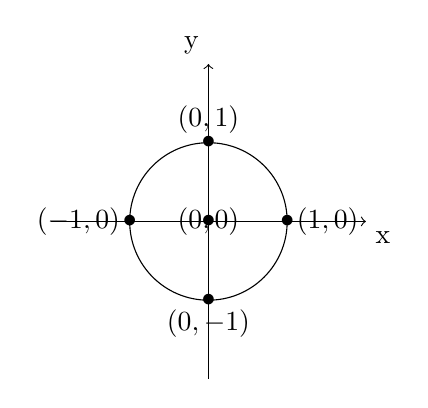
\begin{tikzpicture}
	\pgfmathsetmacro\MAX{2}
	\draw[->] (-\MAX,0) -- (\MAX,0) node[anchor=north west] {x};
	\draw[->] (0,-\MAX) -- (0,\MAX) node[anchor=south east] {y};
	\draw node at (0,0) {$(0,0)$};
	\draw node at (0,0) {$\bullet$};
	\draw node at (0,1) {$\bullet$};
	\draw node at (0,1) [anchor=south]{$(0,1)$};
	\draw node at (1,0) {$\bullet$};
	\draw node at (1,0) [anchor=west] {$(1,0)$};
	\draw node at (-1,0) {$\bullet$};
	\draw node at (-1,0) [anchor=east] {$(-1,0)$};
	\draw node at (0,-1) {$\bullet$};
	\draw node at (0,-1) [anchor=north]{$(0,-1)$};
	\draw (0,0) circle (1);
	\end{tikzpicture}\\
	Per prima cosa osservo che s possono trovare dei punti che rendono vera $f(x,y)=x^2+y^2-1=0$ e sono tutti i punti della circonferenza di centro l'origine degli assi e raggio unitario.\\
	il punto $(x_0,y_0)=(0,1)$ definisce implicitamente una funzione $y=\varphi(x)=\sqrt{1-x^2}$ con $\mathcal{X}=[-1,1]$ e $\mathcal{Y}=[0,1]$\\
	un primo problema è dovuto alla scelta degli intervalli $\mathcal{X},\mathcal{Y}$, per esempio posso scegliere $\mathcal{X}=[-\frac{1}{2},\frac{1}{2}]$ e $\mathcal{Y}=R^+$\\
	un secondo problema è la scelta del punto $(x_0,y_0)$, potrei scegliere il punto $(\frac{1}{\sqrt{2}},\frac{1}{\sqrt{2}})$\\
\observation
La stessa definizione può essere riscritta con la $x$ funzione della $y$ poiché a priori non c'è distinzione tra le variabili.
\proposition (caso lineare)\\
sia $f:R^n\times \R^m\rightarrow \R^p$ che $(x,y)\rightarrow Ax+By-C$ con $A\in Mat(p \times n), B\in (p \times m), B\in (p \times 1)$. Se $p=m$ cioè $B$ è un matrice quadrata, e $det(B)\ne 0$ cioè invertibile, allora\\
$\exists !\varphi : \R^n\rightarrow \R^m$ t.c.: $f(x,y)=0 \iff y=\varphi(x)$
\begin{proof}
	$f(x,y)=0\iff Ax+By=-C\iff By=-Ax+C\iff y=-B^{-1}Ax+B^{-1}C = \varphi(x)$
\end{proof}
\begin{theorem}[Teorema della Funzione Implicita]
	\label{teo:funz_impl}
	Sia $f:X\times Y\rightarrow \R^m$ con $X\subseteq \R^n, Y\subseteq \R^m$\\
	Preso un punto $(x_0,y_0)$ con $x_0\in \circdot{X}$,$y_0\in \circdot{Y}$\\
	se:
	\begin{enumerate}
		\item $f$ continua in $X\times Y$
		\item $f(x_0,y_0)=0$
		\item $f$ differenziabile rispetto a $y \forall (x,y)\in X\times Y$ e $D_yf(x,y)$ continua.
		\item $D_yf(x_0,y_0)$ invertibile .
	\end{enumerate}
	$\Rightarrow $ si ha:\\
	esistenza della funzione implicita\\
	$\exists \mathcal{X}\subseteq X$ intorno di $x_0$(xstrano aperto)\\
	$\exists \mathcal{Y}\subseteq Y$ intorno di $y_0$(ystrano aperto)\\
	$\exists\varphi$ continua con $\varphi:\mathcal{X}\rightarrow\mathcal{Y}$ t.c. $[\varphi (x_0)=y_0 e] f(x,y)=0, x\in\mathcal{X},y\in\mathcal{Y} \iff y=\varphi(x)$
	unicità di sostanza cioè a meno del dominio:\\
	se $\varphi_i:\mathcal{X}_i\rightarrow\mathcal{Y}_i$ e $x_0\in\mathcal{X}_i,y_0\in\mathcal{Y}_i$\\
	$f(x_0,y_0)=0 \forall x\in\mathcal{X}_i, y\in \mathcal{Y}\iff y=\varphi_i(x)$ con $i=1,2$\\
	Allora $\forall\in\mathcal{X}\cap\mathcal{X}_1\cap\mathcal{X}_2$ vale $\varphi_1(x)=\varphi_2(x)$

	\observation
	Le ipotesi 3 e 4 garantiscono che esiste una approssimazione lineare, l'ipotesi 4 è sensata poiché $y$ e $f$ hanno lo stesso numero di componenti quindi $Dyf$ è un matrice qudrata.\\
	la funzione $f:X\times Y\rightarrow \R^m$ che $(x,y)\rightarrow f(x,y)$ ??????\\
	cioè $\forall x\in X$ (sto fissando una x) $f^x:Y\rightarrow \R^m$ che $y\rightarrow f(x,y)$(sto variando la y), $Df^x\in Mat(m\times m)$

	\observation Metodo degli zeri di Newton per troare gli zeri di una funzione o metofo delle tangenti.\\
	\resizebox {\columnwidth} {!} {
	\begin{tikzpicture}
	\draw[->] (-1,0) -- (5,0) node[anchor=north west] {y};
	\draw[->] (0,-1) -- (0,4) node[anchor=south east] {z};
	\draw[domain=-1:4,smooth,variable=\x,blue] plot ({\x},{(1/8)*(\x*\x)-(\x)+1.9});
	\end{tikzpicture}
	}\\
	Scelgo un punto $y_0$ ne prendo il valore sulla curva, disegno la tangente e chiamo $y_1$ l'intersezione con l'asse $y$. Itero il processo $y_n+1=y_n\frac{f(y_n)}{f'(y_n)}$\\
	discorso al momento difficile per me....\\
	\begin{proof}
		Dobbiamo partire da $f(x,y)=0$ arrivare a $y=\varphi(x)$,vogliamo applicare un raginamento simile a quello della Metodo di Newton, passando però per il concetto di punto fisso, il teorema delle Contrazioni ci assicura che esiste unico.\\
		cerchiamo quindi una contrazione $T$ il cui punto fisso sia soluzione di $f(x,y)=0$. $T$ è del tipo:\\
		$T:?\times ?\rightarrow ?$\\
		$(x,y)\rightarrow y-[D_yf(X_0,y_0)]^{-1}f(x,y)$, nota che non avere nella derivata lo stesso punto in cui si calcola la funzione (come è nel metodo di Newton) ha effetti "tragici" sulla velocità di convergenza, ma a noi interessa l'esistenza.\\
		bisgna capire quali insiemi usare come insiemi di partenza e arrivo, devo essere scelti in modo da poter applicare il teoremma delle contrazioni. Bisogna scegliere sottoinsiemi di $R^n$ e $R^m$, scegliamo quindi delle sfere\\
		$T:\overline{B(x_0,r_x)}\times\overline{B(y_0,r_y)}\rightarrow\overline{B(y_0,r_y)}$, scegliendo la chiusura delle sfere si è sicuri di lavorare in uno spazio metrico completo, poiché in $R^l$ completo $\iff$ chiuso e limitato.\\
		come vengono invece scelti i raggi? sono scelti in modo che:\\
		\begin{enumerate}
			\item $T$ è ben definita
			\item $\forall x \in \overline{B(x_0,r_x)} Tx: \overline{B(x_0,r_x)}\rightarrow\overline{B(y_0,r_y)}$ che $y\rightarrow T(x,y)$,\\
		\end{enumerate}
		cioè $T$ è una contrazione tale che $\forall x$ esiste un punto fisso, $\forall x$ associo a $y$ una x, e quindi na funzione.\\
		$r_x,r_y$ devono essere sufficientemene piccoli per avere tali proprietà e per poterci lavorare sopra.\\
		Abbiamo che $f(x,y)=0 \iff T(x,y)=y$\\
		$T(x,y)=y\iff y=y-[D_yF(x_0,y_0)]^{-1}f(x,y)$\\
		$[D_yF(x_0,y_0)]^{-1}f(x,y)\iff f(x,y)=0$\\
		Per verificare che $T$ è una contrazione ne stimo la norma\\
		$\norm{T(x,y_2)-T(x,y_1)} \le \sup\limits_{\widetilde{y}\in segmento}\norm{D_yT(x,\widetilde{y})}\norm{y_2-y_1} $  accrescimenti finiti.\\
		Poichè le sfere sono insiemi convessi è stato possibile applicare il Teorema degli accresscimenti finiti.\\
		Presa $T(x,y) = y-[D_yf(x_0,y_0)]^{-1}f(x,y)$, la derivo rispetto a $y$:
		\[D_yT(x,y)= I_\R^m-[D_yf(x_0,y_0)]^{-1}D_yf(x,y) = \]
		\[=[D_yf(x_0,y_0)]^{-1}][D_yf(x_0,y_0)-D_yf(x,y)]\]
		Osserviamo che abbiamo ottenuto una matrice come costante moltiplicativa, al secondo membro abbiamo la differenza di due valori di una funzione, che per ipotesi è una funzione continua ($D_yf(x,y)$ continua), allora per $r_x$ e $r_y$ sufficientemente piccoli ho che:\\
		$\norm{D_yT(x,y)} \le \frac{1}{2}$, è scelto questo valore poiché è comodo al fine di dimostrare la contrazione...\\
		\[\norm{D_yT(x,y)} \le \norm{D_yf(x_0,y_0)]^{-1}} \norm{D_yf(x_0,y_0)-D_yf(x,y)}\le\frac{1}{2} \]  
		\[\norm{T(x,y_2)-T(x,y_1)}\le\frac{1}{2}\norm{y_2-y_1} \]
		Se dimostriamo che $T$ è ben definita abbiamo dimostrato che $T$ è una contrazione.\\
		Per verificare che $T$ è en definita bisogna mostrare che $T(x,y)\subseteq\overline{B(y_0,r_y)}$ quindi si mostra che la distanza tra $T(x,y)$ e il centro è minore di $r_y$
		\[\norm{T(x,y) - y_0}\le\norm{T(x,y)-T(x,y_0)}+\norm{T(x,y_0)-y_0} \le\]
		\[\le\frac{1}{2}\norm{y-y_0}+\norm{y_0-[D_yf(x_0,y_0)]^{-1}f(x,y_0)-y_0}\le\]
		\[\le\frac{1}{2}\norm{y-y_0}+\norm{[D_yf(x_0,y_0)]^{-1}} \norm{f(x,y_0)-0}\le\]
		\[\le\frac{1}{2}\norm{y-y_0}+\norm{[D_yf(x_0,y_0)]^{-1}} \norm{f(x,y_0)-f(x_0,y_0)}\le\]
		\[\le\frac{1}{2}r_y+\frac{1}{2}r_y\le r_y\]
		Allora $T$ è ben definita perché $T(x,y)\in\overline{B(y_0,r_y)}$.\\
		In conclusione con $\mathcal{X}=\overline{B(x_0,r_x)}$ e $\mathcal{Y}=\overline{B(y_0,r_y)}$ ho che $T:\mathcal{X}\times\mathcal{Y}\rightarrow\mathcal{Y}$ è tale che $\forall x\in\mathcal{X}$ la funzione $y\rightarrow T(x,y)$ è una contrazione e $\overline{B(y_0,r_y)}$ è completo.\\
		quaolcosa sui completi.........\\
		................................\\
		..........................\\
		A questo punto può essere applicato il teorema delle contrazioni:\\
		$\forall x \in \mathcal{X}, \exists y \in\mathcal{Y}: f(x,y)=0$ allora chiamo $\varphi:\mathcal{X}\rightarrow\mathcal{Y}$ che $x\rightarrow y$ è unica quindi $\varphi$ è una funzione.\\
		Allora la funzione implicita esiste. La continuità direva direttamente dal teorema delle contrazioni: l'applicazione che al parametro associa il punto fisso è continua.\\
		Per l'unicità si osservano le ipotesi 1 e 2, dove è scritto $\forall x$ ovvero scelta una qualunque $x$ la $y$ è unica quindi $\varphi$ è univocamente definita.
		
	\end{proof}
\end{theorem}
\proposition
Sia $f:X\times Y\rightarrow \R^m$ con $X\in \R^n, Y\in \R^m$\\
Preso un punto $(x_0,y_0)$ con $x_0\in \circdot{X}$,$y_0\in \circdot{Y}$\\
se:
\begin{enumerate}
	\item $f(x_0,y_0)=0$
	\item $f\in \cntclass{1}(X\times Y,R^m)$.
	\item $D_yf(x_0,y_0)$ invertibile .
\end{enumerate}
$\Rightarrow $ si ha:\\
\begin{enumerate}
	\item $\exists \varphi: \mathcal{X}\rightarrow\mathcal{Y}$ definita implicitamente da $f(x_0,y_0)=0$
	\item $\varphi$ continua su $\mathcal{X}$
	\item $\varphi$ è differenziabile e $D\varphi(x)=-[D_yf(x,\varphi(x))]^{-1}D_xf(x,\varphi(x))$
\end{enumerate}
\begin{proof}
	I punti 1 e 2 sono gli stessi del teorema della funzione implicita e si dimostrano allo stesso modo.\\
	Per il punto 3 abbiamo che $f(x,y)=0\iff y=\varphi(x)$ e quindi $\forall x\in \mathcal{X}$ $f(x,\varphi(x))=0$\\
	.........\\
	.........\\
	
\end{proof}

\proposition CASO N=1, M=1\\
Sia $f:X\times Y\rightarrow \R$ con $X\in \R, Y\in \R$\\
Preso un punto $(x_0,y_0)$ con $x_0\in \circdot{X}$,$y_0\in \circdot{Y}$\\
se:
\begin{enumerate}
	\item $f(x_0,y_0)=0$
	\item $f\in \cntclass{1}(X\times Y,R)$.
	\item $\partial_yf(x_0,y_0)\ne 0$.
\end{enumerate}
$\Rightarrow $ si ha:\\
\begin{enumerate}
	\item $\exists \varphi: \mathcal{X}\rightarrow\mathcal{Y}$ definita implicitamente da $f(x_0,y_0)=0$
	\item $\varphi\in \cntclass{0}(\mathcal{X},\mathcal{Y})$
	\item $\varphi$ è derivabile e $\varphi'(x)=-[\partial_yf(x,\varphi(x))]^{-1}\partial_xf(x,\varphi(x))$
\end{enumerate}
\begin{proof}
	$f(x,y)=0\iff y=\varphi(x)$, derivando $D(f(x,\varphi(x)))=0$\\
	$\partial_xf(x,\varphi(x))+\partial_yf(x,\varphi(x))\varphi'(x)=0$\\
	allora $\varphi'(x) = -\frac{\partial_xf(x,\varphi(x))}{\partial_yf(x,\varphi(x))}$
\end{proof}
\observation Non essendoci motivo per preferire la $x$ alla $y$ o viceversa, esiste anche una versione di questo teorema  in  cui le ipotesi sono le stesse eccetto l'ultima che diventa $\partial_xf(x_0,y_0)\ne 0$
\begin{enumerate}
	\item $\exists \psi: \mathcal{Y}\rightarrow\mathcal{X}$ definita implicitamente da $f(x,y)=0$
	\item $\psi\in \cntclass{0}(\mathcal{Y},\mathcal{X})$
	\item $\psi$ è derivabile e $\psi'(y)=-[\partial_xf(\psi(y),y)]^{-1}\partial_yf(\psi(y),y)$
\end{enumerate}
Qualche esempio qui\\
\subsection{Il Teorema della funzione Inversa}
Data una funzione f, poterla invertire  ...... unico modo l'equazione (o sistema ....)... l'incognita $x$ in funzione del parametro .....\\
\proposition(Teorema della funzione inversa caso lineare)\\
Sia $f:R^n\in \R^m$ data da $f(x)=Mx$ e $M\in Mat(m\times n)$, $f$ è invertibile $\iff n=m$ e $detM\ne 0$
\proposition(caso generale)\\
sia $f:A\rightarrow \R^n$ con $A\in \R^n$, $f\in \cntclass{1}(A,R^n)$, $x_0\in \circdot{A}$ e $Df(x_0)$ invertibile.\\
Allora $\exists\mathcal{X}\in A,\exists\mathcal{Y}\in \R^n$, $\exists\varphi\mathcal{Y}\rightarrow\mathcal{X}$ con la proprietà $f(x)=y\iff x=\varphi(y)$ con $x\in\circdot{\mathcal{X}}$ e $y\in\circdot{\mathcal{Y}}$ e $\varphi\in \cntclass{1}(\mathcal{Y},\mathcal{X})$ e $D\varphi(y)=[Df(x)]^{-1}$\\
\begin{proof}
	$f(x)=y\iff f(x)-y=0$. Allora introduco $F:A\times \R^n\rightarrow \R^n$ data da $F(x,y)=f(x)-y$.\\
	Studio $F(x,y)=0$ per ottenere $x=\varphi(y)$.\\
	Per poter applicare il teorema della funzione implicita serve $D_xF(x_0,y_0)$ invertibile, ma $D_xF(x_0,y_0)=Df(x_0)$ che è invertibile per ipotesi.\\
	Applico allora il teorema della funzione implicita , quindi gli intorni esistono e $x=\varphi(y)$.\\
	resta da trovare la derivata totale di $\varphi$. Sappiamo che $f\in \cntclass{1}$ quindi $\varphi \in \cntclass{1}$.\\
	Sappiamo che $\varphi(f(x))=x$, applicando la derivata della funzione composta abbiamo che:\\
	$D\varphi(f(x))Df(x)=I$\\
	$D\varphi=[Df(x)]^{-1}$ quando $\varphi(y)=x$\\
	si puo anche scrivere come $(Df^{-1})(f(x))=[Df(x)]^{-1}$
\end{proof}
\section{Massimi e Minimi Liberi}
\definition
Siano $(X,d)$s.m., $A\subseteq X$ e $f:A\rightarrow \R$, siano $x_0\in A, B\in A$ e $m,M\in \R$ ( L'insieme immagini deve essere $R$ per poter parlare di massimi e minimi, $R$ è un campo ordinato a differenza di $R^n$).\\
$M$ è massimo di $f$ su $B \bydef M=\max f(B)\iff\forall x \in B f(x_0)\ge f(x)$\\
$M$ è minimo di $f$ su $B \bydef m=\min f(B)\iff\forall x \in B f(x_0)\le f(x)$\\
$x_0$ è punto di massimo assoluto per $f \bydef f(x_0)=\max\limits_{A}f(x)$\\
$x_0$ è punto di minimo assoluto per $f \bydef f(x_0)=\min\limits_{A}f(x)$\\
$x_0$ è punto di massimo locale relativo per $f \bydef \exists r>0: f(x_0)=\max\limits_{x\in B(x_0,r)}f(x)$ con $B(x_0,r)\subseteq A$\\
$x_0$ è punto di minimo locale relativo per $f \bydef \exists r>0: f(x_0)=\min\limits_{x\in B(x_0,r)}f(x)$ con $B(x_0,r)\subseteq A$\\
\subsection{Condizioni Necessarie}
\proposition{Teorema di Fermat}\\
sia $f:A\subseteq \R^n\rightarrow \R$ e $x_0\in\circdot{A}$. Se $x_0$ è punto di massimo(0 minimo) locale per $f$ su $A$ e $f$ è differenziabile in $x_0$ allora $\nabla f(x_0)=0$.
\begin{proof}
	Sia $v\in \R^n$ con $\norm{v} =1$, la funzione $F(t)= f(x_0+tv)$ che a $t\rightarrow x_0+tv$ è il moto rettilineo uniforme che passa da $x_0$ all'istante $0$ e si muove con velocità vettore costante $v$. cioè per tempi negativi mi avvicino a $x_0$ al tempo zero si è in $x_0$ e per tempi positivi si allontana da $x_0$. quindi $t=0$ è punto di massimo per $F$, allora $F'(0) = 0$ per il teorema di Fermat di A1.\\
	Ora abbiamo che $F'(t)=\nabla f(x_0+tv)v$ quindi $F'(0)=\nabla f(x_0)v$ cioè $\nabla f(x_0)v=0$.\\
	Quindi $\forall v :\norm{v} =1$ vale $\nabla f(x_0)=0$\\
	OSS:: Vale anche che $D_vf(x_0)=0$
\end{proof}
\definition
sia $f:A\subseteq r^n\rightarrow \R$, $x_0\in\circdot{A}$\\
$x_0$ è punto stazionario .... $\bydef$ $f$ è differenziabile in $x_0$ e $\nabla f($ ......
\observation
nel caso $n=2, m=1, \nabla f(x_0,y_0)=[\partial_xf(x_0,y_0), \partial_yf(x_0,y_0)]$ ..... i punti stazionari sono quelli che ......parziali.
\observation
Prima di continuare un paio di osservazioni sulle forme quadratiche.\\
\definition
forma quadratica su $R^n \bydef q:R^n\rightarrow \R$ che $x\rightarrow x^TQx$ con $Q\in Mat(n\times n)$ simmetrica\\
ESEMPI:n=2\\
\[
Q=\begin{bmatrix}1&&0\\0&&1\end{bmatrix}\quad
Q=\begin{bmatrix}-1&&0\\0&&-1\end{bmatrix}\quad
Q=\begin{bmatrix}-1&&0\\0&&1\end{bmatrix}\quad 
\]
SEMPRE POSITIVA SEMPRE NEGATIVA CAMBIA SEGNO\\
SEMPRE POSITIVA SEMPRE NEGATIVA CAMBIA SEGNO\\
SEMPRE POSITIVA SEMPRE NEGATIVA CAMBIA SEGNO\\
\proposition
se $Q$ è una forma quadratica, allora\\
\begin{itemize}
	\item $\forall\lambda\in \R, \forall x\in \R^n$ $q(\lambda x)=\lambda^2q(x)$
	\item $q(0)=0$
	\item se $q$ è limitata $\Rightarrow q\equiv 0$ 
\end{itemize}
\begin{proof}
	\begin{itemize}
		\item $q(\lambda x)=(\lambda x)^TQ(\lambda x)=\lambda^2x^TQx=\lambda^2q(x)$
		\item $q(0)=q(0x)=0q(x)=0$
		\item (contronominale $q\ne 0 \Rightarrow q$ non è limitata).\\
		se $q$ è non nulla $\Rightarrow \exists x \in \R^n$ $q(x)\ne 0$\\
		allora $q(\lambda x)=\lambda^2q(x)$ illimitata.
		\item ???????????????????????????????????????????????
	\end{itemize}
\end{proof}
\proposition
se $q$ è una forma quadratica $\Rightarrow\exists M\ge 0: \abs{q(x)}\le M\norm{x}^2$ $\forall x\in \R^n$
\begin{proof}
	per $x\ne 0$ $\abs{q(x)} =\abs{q\left(\norm{x} \frac{1}{\norm{x} }x\right)} = \norm{x}^2\abs{q\left(\frac{1}{\norm{x}}x\right)}\le$\\
	$\le\left(\sup\limits_{\norm{x}=1}\abs{q(x)}\right)\norm{x}^2=\le\left(\max\limits_{\norm{x}=1}\abs{q(x)}\right)\norm{x}^2=M\norm{x}^2$
\end{proof}
\proposition
Sia $q$ una forma quadratica, se $q(x)=o(\norm{x}^2)$ per $x\rightarrow 0 \Rightarrow q\equiv 0$
\begin{proof}
	sia $x\in \R^n$ con $\norm{x}=1$ e $t>0$.\\
	$q(x)=\frac{1}{t^2}$, $q(tx)=\frac{q(tx)}{\norm{tx}^2}\rightarrow 0$ per $t\rightarrow 0$ per ipotesi.\\
	Allora $\forall x$ con $\norm{x}$ vale $q(x)=0$ e allora $\forall x\ne 0, q(x)=q\left(\frac{1}{\norm{x}}x\right)\norm{x}^2$
\end{proof}
\definition
Sia $q:R^n\rightarrow \R$ una forma quadratica\\
\begin{itemize}
	\item $q$ è definita positiva $\bydef \forall x\in \R^n, x\ne 0$ $q(x)>0 [Q>0]$
	\item $q$ è semidefinita positiva $\bydef \forall x\in \R^n$ $q(x)\ge0 [Q\ge0]$
	\item $q$ è definita negativa $\bydef \forall x\in \R^n, x\ne 0$ $q(x)<0 [Q><0]$
	\item $q$ è semidefinita negativa $\bydef \forall x\in \R^n$ $q(x)\le0 [Q\le0]$
\end{itemize}
\proposition
Sia $q:R^n\rightarrow \R$ una forma quadratica, se $q$ è definita positiva $\Rightarrow \exists m>0: \forall x \in \R^n, q(x)\ge m\norm{x}^2$
\begin{proof}
	Noto che $q(\lambda x)=\lambda^2q(x)$\\
	$q(x)=q\left(\frac{1}{\norm{x}}x\norm{x}^2\right)\ge\min\limits_{\norm{x}=1}q(\lambda)\norm{x}^2$
\end{proof}
Ora dobbiamo cercare di capire se $q$ è definita positiva\\
Ad esempio: $Q=\begin{bmatrix}1&&0&&0\\0&&-1&&0\\0&&0&&0\end{bmatrix}$ è facile capire che è semodefinita positiva poiché è in diagonale, quindi la prima cosa da fare è trovare una forma diagonale per $Q$\\
un procedimento pratico e veloce è il seguente:\\
\[Q=\begin{bmatrix}q_{11}&&q_{12}&&q_{13}&&\ldots\\q_{21}&&q_{22}&&q_{23}&&\ldots\\q_{31}&&q_{32}&&q_{33}&&\ldots\\\vdots&&\vdots&&\vdots&&\ddots\end{bmatrix}\rightarrow\begin{bmatrix}\lambda_{1}&&0&&0&&\ldots\\0&&\lambda_{2}&&0&&\ldots\\0&&0&&\lambda_{3}&&\ldots\\\vdots&&\vdots&&\vdots&&\ddots\end{bmatrix}\]
\[\lambda=q_{11},\quad\lambda_{2}=\frac{detQ_2}{q_11}\quad\lambda_{3}=\frac{detQ_3}{detQ_2}\quad ...\quad \lambda_{i}=\frac{detQ_i}{detQ_{i-1}}\]
Questo perché se dobbiamo valutare il segno dell'incremento della f ci servono le variazioni sulle quadriche. Se $f$ è $\cntclass{2}$ scrivo lo sviluppo di Taylor al secondo ordine:\\
\[f(x)-f(x_0)=\nabla f(x_0)(x-x_0)+\frac{1}{2}(x-x_0)^TH_f(x_0)(x-x_0)+o(\norm{x-x_0}^2)\]
max e min dove $\nabla f(x_0)=0$ per Fermat, l'o piccolo è trascurabile, allora il segno della derivata dipende dalla forma quadratica al secondo membro.
\proposition
sia $f:A\subseteq \R^n\rightarrow \R$ e $x_0\in\circdot{A}$.\\
$f\in \cntclass{2}(A;R)$ e $x_0$ punto di massimo locale per $f$ su $A\Rightarrow\nabla f(x_0)=0$ e $H_f(x_0)$ è semidefinita negativa.
\begin{proof}
	$f(x)-f(x_0)=\frac{1}{2}(x-x_0)^TH_f(x_0)(x-x_0)+o(\norm{x-x_0}^2)$ poiché $f\in \cntclass{2}$\\
	il primo termine è negativo poiché per ipotesi $x_0$ è punto di massimo locale, ne segue che il termine $(x-x_0)^TH_f(x_0)(x-x_0)$ non può essere positivo. 
\end{proof} 
\proposition
sia $f:A\subseteq \R^n\rightarrow \R$ e $x_0\in\circdot{A}$.\\
$f\in \cntclass{2}(A;R)$ e $x_0$ punto di minimo locale per $f$ su $A\Rightarrow\nabla f(x_0)=0$ e $H_f(x_0)$ è semidefinita positiva.
\begin{proof}
	$f(x)-f(x_0)=\frac{1}{2}(x-x_0)^TH_f(x-x_0)+o(\norm{x-x_0}^2)$ poiché $f\in \cntclass{2}$\\
	il primo termine è positivo poiché per ipotesi $x_0$ è punto di minimo locale, ne segue che il termine $(x-x_0)^TH_f(x-x_0)$ non può essere negativo. 
\end{proof} 


\subsection{Condizioni Sufficienti}
\proposition
sia $f:A\subseteq \R^n\rightarrow \R$ e $x_0\in\circdot{A}$.\\
$f\in \cntclass{2}(A;R)$, $\nabla f(x_0)=0$,$H_f(X_0)$ è definita negativa $\Rightarrow x_0$ è un punto di massimo locale per $f$
\begin{proof}
	$f\in \cntclass{2}$ quindi possiamo scrivere:\\
	$f(x_+h)-f(x_0)=\nabla f(x_0)h+\frac{1}{2}(h)^TH_f(x_0)+o(\norm{h}^2)$ per $h\rightarrow 0$\\
	$f(x_+h)-f(x_0)=\frac{1}{2}(h)^TH_f(x_0)+o(\norm{h}^2)$ per $h\rightarrow 0$\\
	Sappiamo che $H_f$ è definita negativa per ipotesi, allora $h^TH_f(x_0)h\le -m\norm{x_0}$ allora $f(x_0+h)-f(x_0)<0$ e quindi $x_0$ è punto di massimo locale per $f$.
\end{proof} 
\proposition
sia $f:A\subseteq \R^n\rightarrow \R$ e $x_0\in\circdot{A}$.\\
$f\in \cntclass{2}(A;R)$, $\nabla f(x_0)=0$,$H_f(X_0)$ è definita positiva $\Rightarrow x_0$ è un punto di minimo locale per $f$
\begin{proof}
	$f\in \cntclass{2}$ quindi possiamo scrivere:\\
	$f(x_+h)-f(x_0)=\nabla f(x_0)h+\frac{1}{2}(h)^TH_f(x_0)+o(\norm{h}^2)$ per $h\rightarrow 0$\\
	...........\\
	...........\\
\end{proof} 
QUALCHE DISEGNO E SPIEGAZIONE.....
\subsection{Il Significato Geometrico del Gradiente n=2 m=1}
\definition
Sia $A\subseteq \R^2$ e $f:A\rightarrow \R$\\
La suferficie $z=f(x,y)$ è il grafico di $f$, è unsottoinsieme di $R^3$\\
Se $c\in \R$, la curva di livello $c$ di $f$ è l'insieme $f^{-1}(c)\{(x,y)\in A: f(x,y)=c\}$\\
Se $f$ 	'e differenziabile in $(x_0,y_0)\in\circdot{A}$ il piano tangente alla superficie $z=f(x,y)$ in $(x_0,y_0)$ ha equazione:\\
\[z=f(x_0,y_0)+\nabla f(x_0,y_0)\begin{bmatrix}(x-x0)\\(y-y_0)\end{bmatrix}\] 
\[z=f(x_0,y_0)+\partial_xf(x_0,y_0)(x-x_0)+\partial_yf(x_0,y_0)(y-y_0)\]
\observation
geometricamente, il gradiente di una funzione indica la direzione di $R^n$ in cui si ha la massima variazione del valore di f, nel verso di incremento positivo di $f$,
\observation 
osservazione col grafico che al momento non faccio.
\proposition
Siano $A\subseteq \R^n, f:A\rightarrow \R$ differenziabile in $(x_0,y_0)\in \circdot{A}$, l'incremento di $f(x_0+h,y_0+k)-f(x_0,y_0)$ è massimo quando $[h k]=\lambda\nabla f(x_0,y_0)$ con $\lambda >0$ ed è minimo con $[h k]=\lambda\nabla f(x_0,y_0)$ con $\lambda <0$
\begin{proof}
	so che posso approssimare la funzione quindi posso scrivere:\\
	$f(x_0+h,y_0+k)-f(x_0,y_0)=\nabla f(x_0,y_0)\begin{bmatrix}h\\k\end{bmatrix}+o(\sqrt{h^2+k^2})$=
	$=\norm{\nabla f(x_0,y_0)}\norm{\begin{bmatrix}h k\end{bmatrix}}cos(\theta)+o(\sqrt{h^2+k^2})$\\
	dove $\theta$ è l'angolo tra $\nabla f(x_0,y_0)$ e $[h k]$ per $||[h k]||$ sufficientemente piccola, l'incremento $f(x_0+h,y_0+k)-f(x_0,y_0)$ è massimo se $cos( \theta )=1$ ed è minimo se $cos(\theta )=-1$, da cui la tesi.\\ 
\end{proof}
\proposition
siano $f\in \cntclass{1}(A;R)$ con $A\subseteq \R^2$ e $(x_0,y_0)\in\circdot{A}$ e $\nabla f(x_0,y_0)\ne 0$[cioè stazionario]. Allora $nabla f(x_0,y_0)$ è perpendicolare alla curva di livello passante per .....
\observation
un vettore 1'e perpendicolare a una curva se è perpendicolare alla retta o al vettore tangente alla curva in quel punto.
\begin{proof}
	La curva di livello è $f(x,y)=f(x_0,y_0)$ cioè $f(x,y)-f(x_0,y_0)=0$, per trovare la tangente a questa curva è piu facile se si ha $y=\varphi(x)$\\
	Usiamo quindi il teorema della funzione implicita, mi serve che $\partial_yf(x_0,y_0)\ne 0$, questa condizione non è assicurata dalle ipotesi, per ipotesi il gradiente è non nulla quindi almeno una delle due componenti è non nulla.\\
	Inizio con il caso $\partial_yf(x_0,y_0)\ne 0$.\\
	Il T.F.IMPL. assicura che :\\
	$\exists\mathcal{X},\mathcal{Y}$ con $x_0\in\circdot{\mathcal{X}}, y_0\in\circdot{\mathcal{Y}}$, $\exists\varphi:\mathcal{X}\rightarrow\mathcal{Y}$ t.c.:\\
	$f(x,y)=f(x_0,y_0), x\in\mathcal{X}, y\in\mathcal{Y} \iff y=\varphi(x)$\\
	La retta tangente in $x_0$ a $y=\varphi(x)$ è $y=y_0+\varphi'(x_0)(x-x_0)$\\
	questo vuole dire che un vettore tangente a $y=\varphi(x)$ in $(x_0,y_0)$ è $\begin{bmatrix}1\\\varphi'(x_0)\end{bmatrix}$.\\
	... calcolo il prodotto scalare\\
	\[\nabla f(x_0,y_0)\begin{bmatrix}1\\\varphi'(x_0)\end{bmatrix} = \begin{bmatrix}\partial_x f(x_0,y_0)&&\partial_y f(x_0,y_0)\end{bmatrix}\begin{bmatrix}1\\-\frac{\partial_x f(x_0,y_0)}{\partial_y f(x_0,y_0)}\end{bmatrix} =\] 
	\[=\partial_x f(x_0,y_0) -\partial_y f(x_0,y_0)\frac{\partial_x f(x_0,y_0)}{\partial_y f(x_0,y_0)}=0\]
	Allora il graadiente è perpendicolare alla curva di livello.\\
	Guardiamo ora al caso in cui $\partial_yf(x_0,y_0)= 0$ e $\partial_xf(x_0,y_0)\ne 0$ quindi il gradiente è non nullo.\\
	Applicando lo stesso ragionamento id sopra, solo esplicitando la $x$ in funzione della $y$. Quindi $x=\psi(x)$ e $\psi{'}(y_0)=-\frac{\partial_y f(x_0,y_0)}{\partial_x f(x_0,y_0)}$
\end{proof}

\section{Massimi e Minimi Vincolati}
Spesso la ricerca di punti di massimo o minimo di una funzione $f:A\rightarrow \R, A\subseteq \R^n$ deve essere ristrettaad un sottoinsieme $B\subseteq A$ a causa di eventuali vincoli a cui le variabili indipendenti devono soddisfare. L0insieme $B$ può essere generalmente descritto da una funzione $\varphi :A\rightarrow \R^p$, nel senso che $B=\{x\in A:\varphi (x)\le 0\}$\\
NOTA::: direi n>1 poiché se ho una sola variabile e la vincolo ...??????? booooo .\\
Questo problema è usualmente abbreviato in:
\[\max\limits_{\varphi \le 0}\quad o \quad\min\limits_{\varphi \le 0}\]
può essere affrontato in due passi:\\
\begin{enumerate}
	\item ricerca dei punti di estremo di $f$ interni a $B$, problema gia affrontato.
	\item ricerca dei punti di estremo di $f$ sul bordo di $B$, affrontiamo ora.
\end{enumerate}
Sotto opportune condizioni su $\varphi$, infatti, $\circdot{B} = \{x\in A:\varphi(x)<0\}$ e $\partial B\{x\in A:\varphi(x)=0\}$
\proposition{Teorema dei Moltiplicatori di Lagrange}
Siano $f,g:A\subseteq \R^2\rightarrow \R, (x_0,y_0)\in\circdot{A}, g(x_0,y_0)=0, f,g\in \cntclass{1}(A;R)$, $\nabla g (x_0,y_0)\ne 0$\\
Se $(x_0,y_0)$ è di max(o min) locale per $f$ su $g=0\Rightarrow\exists \lambda in \R$ t.c: $\nabla f(x_0,y_0) = \lambda g(x_0,y_0)$ (all fin fine posso dire che sono paralleli).\\
\observation
$\lambda$ si chiama "moltiplicatore di lagrange"
\observation
Se abbiamo un problema del tipo $\max\limits_{g(x,y)=0}f$ cioè il massimo di $f$ sul vincolo $g(x,y)=0$, ci dobbiamo ricondurre ad un sistema del tipo
$\begin{cases} \nabla f(x_0,y_0)=\lambda \nabla g(x_0,y_0)\\ g(x_0,y_0)=0 \end{cases}=\begin{cases} \partial_xf(x_0,y_0)=\lambda \partial_xg(x_0,y_0)\\\partial_yf(x_0,y_0)=\lambda \partial_yg(x_0,y_0)\\ g(x_0,y_0)=0 \end{cases}$\\
3 equazioni in 3 incognite($x,y,\lambda$)\\
In certi casi si introduce una funzione $\mathcal{L}(x,y,\lambda) = f(x,y)-\lambda g(x,y)$ detta Lagrangiana, i punti stazionari vincolati di $f$ sono punti stazonari liberi della Lagrangiana.\\
\begin{proof}
	Sappiamo che $\nabla g(x_0,y_0)\ne$ quindi $\begin{bmatrix}\partial_xg(x_0,y_0) &&\partial_yg(x_0,y_0)\end{bmatrix}\ne\begin{bmatrix}0&&0\end{bmatrix}$ quindi o $\partial_xg(x_0,y_0)\ne 0$ o $\partial_yg(x_0,y_0)\ne 0$.
	Mettiamoci nel caso in cui $\partial_yg(x_0,y_0)\ne 0$,\\
    Per il teorema della funzione implicita ho che :\\
	$\exists\mathcal{X},\mathcal{Y}$ con $x_0\in\circdot{\mathcal{X}}, y_0\in\circdot{\mathcal{Y}}$, $\exists\varphi:\mathcal{X}\rightarrow\mathcal{Y}$ t.c.:\\
	$g(x,y)=f(x_0,y_0), x\in\mathcal{X}, y\in\mathcal{Y} \iff y=\varphi(x)$\\
	Osserviamo che dire $(x_0,y_0)$ di massimo o minimo per $f$ ristretta a $g(x,y)=0\iff x_0$ è di massimo o di minimo per la funzione $x\rightarrow f(x,\varphi(x))$.\\
	Per il teorema di Fermat $\left.\frac{\mathrm{d}}{\mathrm{d}x}(f(x,\varphi(x)))\right\|_{x=x_0}=0$, punto stazionario ha derivata nulla, e la derivata di quella funzione in $x_0$ è:
	\[\partial_xf(x_0,\varphi(x_0))+\partial_yf(x_0,\varphi(x_0))\cdot\varphi'(x_0)\] 
	allora
	\[0=\partial_xf(x_0,\varphi(x_0))+\partial_yf(x_0,\varphi(x_0))\cdot\varphi'(x_0)=\]
	\[=\partial_xf(x_0,\varphi(x_0))-\partial_yf(x_0,\varphi(x_0))\frac{\partial_xg(x_0,\varphi(x_0))}{\partial_yg(x_0,\varphi(x_0))}=\]\\
	\[=\partial_xf(x_0,\varphi(x_0))\partial_yg(x_0,\varphi(x_0))-\partial_yf(x_0,\varphi(x_0))\partial_xg(x_0,\varphi(x_0))=det\left(\begin{matrix}\partial_xf(x_0,y_0)&&\partial_yf(x_0,y_0)\\\partial_xg(x_0,y_0)&&\partial_yg(x_0,y_0)\end{matrix}\right)=0\]\\
	questo equivale a dire che i vettori riga della matrice sono paralleli quindi $\exists\alpha\in \R : \nabla f(x_0,y_0)=\lambda\nabla g(x_0,y_0)$.\\
	Non è uguale scrivere $\exists\alpha\in \R : \nabla g(x_0,y_0)=\lambda\nabla f(x_0,y_0)$ poiché non c'è certezza sul valore di $\nabla f(x_0,y_0)$ che se nullo negherebbe l'ipotesi di $\nabla g(x_0,y_0)\ne 0$\\
	Se guardiamo ora il caso in cui $\partial_yg(x_0,y_0)=0$ e $\partial_xg(x_0,y_0)\ne 0$.\\
	Seguendo un ragionamento analogo si esplicita $x=\psi(y)$ così che cercare max(o min) di $f$ ristretta a $g(x,y)=0$ porti a $y\rightarrow f(\psi(y),y)$ 
\end{proof}
\proposition{Teorema dei Moltiplicatori di Lagrange caso generale}
Sia $A\in \R^n$, $f\in \cntclass{1}(A;R)$, $g\in \cntclass{1}(A;R^p)$ con $p<n$(n.vincoli<n.variabili), sia poi $x_0\in\circdot{A}, g(x_0)=0, Dg (x_0,y_0)$ di rango $p$.\\
Se $x_0$ è di max(o min) locale per $f$ su $g=0\Rightarrow\exists \lambda_1,\ldots,\lambda_p in \R$ t.c: $\nabla f(x_0,y_0) = \sum\limits_{i=1}^{p}\lambda_i\nabla g(x_0,y_0)$\\
\section{Il caso \texorpdfstring{$n=2,\,m=1$}{n=2, m=1}}
%TODO This section is a placeholder
\section{Derivate e Integrali}
\begin{proposition}[Teorema Fondamentale del Calcolo Integrale]
	\label{teo:fondament_calcolo_integ}
	Sia $I\subseteq \R$ un intervallo e sia $x_0\in I$. Data $f\in c^0(I;R)$ la funzione:
	\[\begin{array}{rcl} F: I & \to & \R \\ x & \to & \int_{x_0}^{x}f(t)\integrald{t} \end{array}\]
	Si ha $F\in \cntclass{1}(I;R)$ e $F'(x)=f(x)$ $\forall x \in I$
\end{proposition}[]
\proposition
Sia $A\subseteq \R^n$ un aperto, data $f\in \cntclass{0}(A\times \R;R)$ la funzione \\
$\begin{array}{rcl} F: \R\times \R\times A & \to & \R \\ (\alpha,\beta,x) & \to & \int_{\alpha}^{\beta}f(x,t)\integrald{t} \end{array}$\\
è di classe $\cntclass{0}(R\times \R\times A;R)$
\proposition
Sia $A\subseteq \R^n$ un aperto, data $f\in \cntclass{1}(A\times \R;R)$ la funzione \\
$\begin{array}{rcl} F: \R\times \R\times A & \to & \R \\ (\alpha,\beta,x) & \to & \int_{\alpha}^{\beta}f(x,t)\integrald{t} \end{array}$\\
è di classe $\cntclass{1}(R\times \R\times A;R)$ ed inoltre, $\forall (\alpha,\beta,x)\in \R\times \R\times A$ e $\forall i=1,\ldots,n$\\
\[\frac{\partial F}{\partial \alpha}=-f(x,\alpha)\]
\[\frac{\partial F}{\partial \beta}=f(x,\beta)\]
\[\frac{\partial F}{\partial x_i}=\int_{\alpha}^{\beta}\frac{\partial F}{\partial x_i}(x,t)\integrald{t}\]
\[\nabla F=\int_{\alpha}^{\beta}\nabla f(x,t)\integrald{t}\]
\corollary
Sia $A\subseteq \R^n$ un aperto, date le funzioni $\alpha:x\rightarrow \R, \beta:x\rightarrow \R, f:x\rightarrow \R, $ di classe $\cntclass{1}$ , la funzione \\
$\begin{array}{rcl} F: A & \to & \R \\ (x) & \to & \int_{\alpha(x)}^{\beta(x)}f(x,t)\integrald{t} \end{array}$\\
è di classe $\cntclass{1}(R\times \R\times A;R)$ ed inoltre, $\forall x_0 \in A$:
\[\nabla F(x_0,y_0)=f(x_0,\beta)\nabla\beta(x_0)-f(x_0,\alpha)\nabla\alpha(x_0)+\int_{\alpha(x_0)}^{\beta(x_0)}\nabla f(x,t)\integrald{t}\]

\section{Funzioni a Valori in \texorpdfstring{$\protect\C$}{C}}
\label{sec:fun_in_C}
Sia $A \subseteq \R^n$ non vuoto. Ogni funzione $A \mapsto \C$ può essere identificata in modo naturale con una funzione $A \mapsto \R^2$ e viceversa.ù
\begin{note}
	Quindi è possibile rappresentare una funzione $A \mapsto \C$ in un piano, detto \textbf{piano complesso} o \textbf{piano di Gauss}
\end{note}
\begin{exercise}
	\label{ex:ext_def_in_C}
	Utilizzando questa identificazione, estendere al caso di funzioni $A \mapsto \C$ le definizioni di continuità, derivabilità, differenziabilità e degli spazi $\cntclass{k}$ date per funzioni $A \mapsto \R$
	% TODO solution
\end{exercise}
\begin{proposition}
	\label{prop:fg_in_C}
	Sia $A \subseteq \R$ e sia $t_0 \in \circdot{A}$. Allora
	\begin{itemize}
		\item Se due funzioni $f,g: A \mapsto \C$ sono differenziabili in $t_0$, anche le funzioni $f+g$ e $f \cdot g$ sono differenziabili in $t_0$. Inoltre
			\[(f+g)'(t_0) = f'(t_0) + g'(t_0) \qquad\text{e}\qquad (f \cdot g)'(t_0) = f'(t_0)g(t_0)+f(t_0)g'(t_0)\]
		\item Per ogni $\lambda \in \C$, anche $\lambda f$ è differenziabile e
			\[(\lambda f)'(t_0) = \lambda f'(t_0)\]
		\item Se $g(t_0) \neq 0$, anche $1/g$ e $f/g$ sono differenziabili in $t_0$ e
			\[(1/g)'(t_0) = - \frac{g'(t_0)}{g^2(t_0)} \qquad\text{e}\qquad (f/g)'(t_0) = \frac{f'(t_0)g(t_0)-f(t_0)g'(t_0)}{g^2(t_0)}\]
	\end{itemize}
	\begin{proof}
		Omessa
	\end{proof}
\end{proposition}
\begin{exercise}
	Dimostrare la \fullref{prop:fg_in_C}
	% TODO solution
\end{exercise}
\begin{definition}[Funzione Esponenziale con Esponente Complesso]
	La Funzione Esponenziale con Esponente Complesso è così definita:
	\[e^{x+iy} = e^x \cdot (\cos y + i \sin y)\]
\end{definition}
\begin{proposition}
	\label{prop:deriv_exp_in_C}
	Qualunque sia $\lambda \in \C$,
	\[\frac{d}{dt}e^{\lambda t} = \lambda e^{\lambda t}\]
	\begin{proof}
		Omessa
	\end{proof}
\end{proposition}
\begin{exercise}
	Dimostrare la \fullref{prop:deriv_exp_in_C}, direttamente o attraverso l'\fullref{ex:deriv_func_with_taylor}
\end{exercise}
\begin{exercise}
	In questa sezione sulle funzioni a valori complessi non son stati considerati i problemi di massimo/minimo, perché?
	\begin{solution}
		Perché $\C$ non è ordinato, dunque non è possibile trovare massimi o minimi.
	\end{solution}
\end{exercise}
\chapter{Integrali Doppi}
\newpage
\section*{Preliminari}
Questo capitolo non è trattato in maniera approfondita poiché:
\begin{description}
	\item[a] tanti e lunghi teoremi fuori contesto per poter introdurre rigorosamente la teoria di Riemann
	\item[b] tale teoria è "superata" da tempo
\end{description}
Il primo è più grosso problema di tale teoria è che non permette il passaggio del limite sotto il segno di integrale, cioè per poter scrivere 
\[ \int\lim\limits_{n\to\infty}f_n(x) = \lim\limits_{n\to\infty}\int f_n(x)\] sono necessarie tante ipotesi molto restrittive.\\
Si è passati così alla teoria dell'integrale secondo Lebesgue, molto diversa e piuttosto complicata.\\
ESEMPIO...............\\
disegni...........\\
................\\
Il concetto di integrale è quindi molto legato al concetto di area e anche di volume. La teoria di Lebesgue riparte da assiomi come questi definendoli e caratterizzandoli in modo da definire una volta per tutte in maniera sistematica e rigorosa cosa si può e cosa non si può integrare, e dove ha senso parlare di superfici. volumi, ipervolumi, ... 
\newpage
\section{Regole di Calcolo}
Queste formule permettono di ricondurre il calcolo di integrali doppi a quello di integrali semplici.\\
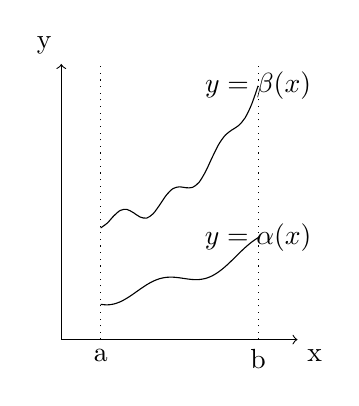
\begin{tikzpicture}
\draw[->] (0,0) -- (3,0) node[anchor=north west] {x};
\draw[->] (0,0) -- (0,3.5) node[anchor=south east] {y};
\draw[dotted] (.5,0) -- (.5,3.5);
\draw[dotted] (2.5,0) -- (2.5,3.5);
\draw (.5,0)  node[anchor=north] {a};
\draw (2.5,0) node[anchor=north] {b};
\draw[domain=.5:2.5,smooth,variable=\x] plot ({\x},{(1/9)*\x*\x*\x+1.5+0.1*sin(10*\x r)}) node {$y=\beta(x)$};
\draw[domain=.5:2.5,smooth,variable=\x] plot ({\x},{(1/9)*\x*\x+0.5+0.1*cos(5*\x r)}) node {$y=\alpha(x)$};
\end{tikzpicture}\\
Se:\\
$a,b\in \R$ con $a<b$\\
$\alpha,\beta\in \cntclass{0}([a,b];R), \forall x\in[a,b] \alpha(x)\le\beta(x)$\\
$A=\{(x,y)\in \R^2: x\in [a,b] $e$ y\in [\alpha(x),\beta(x)] \}$\\
$f\in \cntclass{0}(A;R)$\\
Allora\\
$\iint_Af(x,y)\integrald{x}\integrald{y}=\int_a^b\left(\int_{\alpha(x)}^{\beta{x}}f(x,y)\integrald{y}\right)\integrald{x}$\\
Analogamente.\\
ALTRO GRAFICO....\\
Se:\\
$c,d\in \R$ con $c<d$\\
$\gamma,\delta\in \cntclass{0}([a,b];R), \forall y\in[c,d] \gamma(y)\le\delta(y)$\\
$A=\{(x,y)\in \R^2: x\in [c,d] $e$ x\in [\gamma(y),\delta(y)] \}$\\
$f\in \cntclass{0}(A;R)$\\
Allora\\
$\iint_Af(x,y)\integrald{x}\integrald{y}=\int_c^d\left(\int_{\gamma(y)}^{\delta{y}}f(x,y)\integrald{x}\right)\integrald{y}$
\newpage
\section{Cambiamento di Variabili}
Se:\\
$A\subseteq \R^2$\\
$\varPhi\in \cntclass{1}(A;R^2)$
$\varPhi$ è invertibile
$\varPhi^{-1}\in \cntclass{1}(\varPhi(A);R^2)$\\
$det(D\varPhi)\ne 0$ su $A$\\
$f\in \cntclass{0}(\varPhi(A);R^2)$\\
Allora:\\
\[ \iint_{\varPhi(A)}f(x,y)\integrald{x}\integrald{y}=\iint_A((f\circ g)(u,v))\abs{det(D\varPhi(u,v))}\integrald{u}\integrald{v}\]
La quantità $det(D\varPhi)$ è spesso chiamato DETERMINANTE JACOBIANO (o semplicemente JACOBIANO) della trasformazione $\varPhi$\\
Adesso spieghiamo perché il determinante JACOBIANO, ricordando A1:
\[ \int_g(A)f(x)\integrald{x} = \int_Af(g(t))\integrald{t}\]\\
vari casi\\
...\\
...\\
...\\




\chapter{Successioni e Serie di Funzioni}
\section{Preliminari}
\definition
Sia $f_n:A\subseteq \R\to \R$ una successione ($n\in\N$) , la serie $\sum\limits_{n=09}^{+\infty}f_n$ indica la successione delle somme parziali $S_n = \sum\limits_{i=0}^nf_i$
\observation
Qualunque affermazione fatta in riferimento ad una serie va quindi intesa riferita alla successione delle somme parziali
\begin{description}
	\item[-] La serie è limitata $\bydef$ la successione delle somme parziali è limitata
	\item[-] La serie è illimitata $\bydef$ la successione delle somme parziali è illimitata
	\item[-] La serie è convergente $\bydef$ la successione delle somme parziali è convergente
\end{description}
\observation
Successioni e serie di funzioni possono essere viste:
\begin{enumerate}
	\item come successioni e serie dipendenti da un parametro
	\item come un mezzo per approssimare funzioni
	\item come un primo passo verso lo studio di funzioni (a volte dette operatori o funzionali) che a funzioni associano o numeri o altre funzioni.
\end{enumerate}
\section{Tipi Di Convergenza}
\subsection{Convergenza Puntuale}
\definition
Sia $A\subseteq \R$ e $\left\{f_n:n\in\N\right\}$ una successione di funzioni definite su $A$ a valori in $ \R$. Sia $B\subseteq A$
\begin{description}
	\item[-] la successione $\left\{f_n:n\N\right\}$ è puntualmente convergente su $B$ se $\forall x \in B$, esiste finito il limite $\lim\limits_{n\to\infty}f_n(x)$. In tal caso la funzione $f:B\to  \R$ definito da $f(x)=\lim\limits_{n\to\infty}f_n(x)$
	\item[-] la serie $\sum\limits_{n=0}^{\infty}f_n$ è puntualmente convergente su $B$ se $\forall x \in B$, la serie $\sum\limits_{n=0}^{\infty}f_n(x)$ ammette somma finita. In tal caso la funzione $F:B\to  \R$ definito da $F(x)=\sum\limits_{n=0}^{\infty}f_n(x)$ è la somma della serie la serie $\sum\limits_{n=0}^{\infty}f_n$
\end{description}
\observation
La convergenza puntuale su $A$ della successione $f_n$ verso $f$ è indicata con
$$f_n \pconvarrow f\quad su A$$
\proposition METAPROPOSIZIONE:\\
Sia $f_n:A\to \R$, $B\subseteq A$, $A\subseteq \R$, $f:B\to A$\\
Se $f_n \pconvarrow f$ su $B$ e se $f_n$ ha la proprietà $P$ allora il limite $f$ ha la proprietà $P$.\\

\example $f_n(x)=\frac{1}{n}sin(x)$ con $A\equiv \R$\\
$\lim\limits_{n\to\infty}f_n(x)=\lim\limits_{n\to\infty}\frac{1}{n}sin(x)=0\quad\forall x \in A \Rightarrow f_n \pconvarrow 0$ su $A$.

\example$f_n(x)=e^{nx}$ con $A\equiv \R$
\begin{center}
	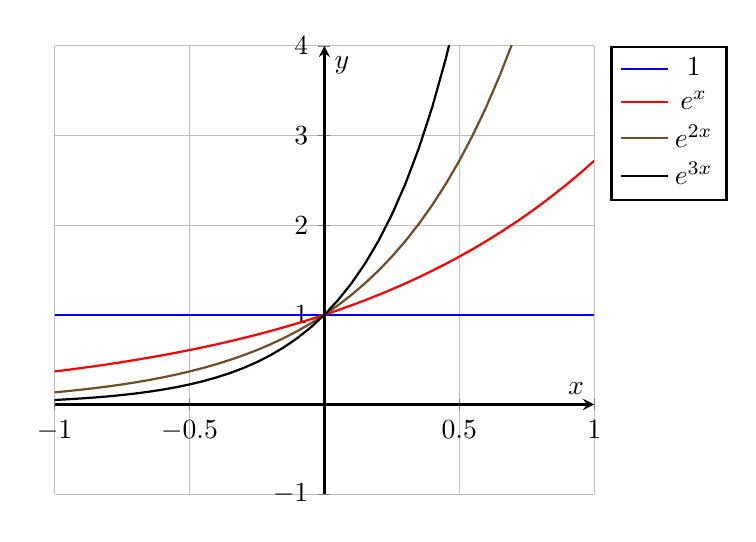
\begin{tikzpicture}[scale=1]
		\begin{axis}[
			xlabel={$x$},ylabel={$y$},
			axis lines=middle,
			samples=41,grid,thick,
			domain=-1:1,
			ymin=-1,ymax=4,
			legend pos=outer north east ]
			\addplot+[no marks] {1}; \addlegendentry{$1$}
			\addplot+[no marks] {e^x}; \addlegendentry{$e^x$}
			\addplot+[no marks]{e^(2*x)}; \addlegendentry{$e^{2x}$}
			\addplot+[no marks]{e^(3*x)}; \addlegendentry{$e^{3x}$}
			\end{axis}
	\end{tikzpicture}
\end{center}
$$\lim\limits_{n\to\infty}e^{nx} = \left\{\begin{matrix} 0 && x<0\\1&&x=0\\\infty&&x>0 \end{matrix}\right.$$
$$f_n \pconvarrow f\quad su B=\left]-\infty,0\right]$$
\observation
La continuità non passa al limite come proprietà $P$

\example $f_n(x)=x^n$ con $A\equiv \R$
\begin{center}
	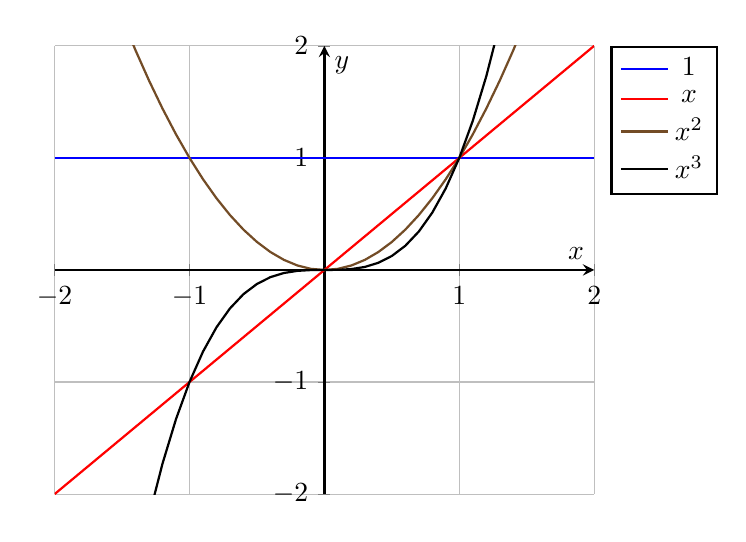
\begin{tikzpicture}[scale=1]
		\begin{axis}[
			xlabel={$x$},ylabel={$y$},
			axis lines=middle,
			samples=41,grid,thick,
			domain=-2:2,
			ymin=-2,ymax=2,
			legend pos=outer north east ]
			\addplot+[no marks] {1}; \addlegendentry{$1$}
			\addplot+[no marks] {x}; \addlegendentry{$x$}
			\addplot+[no marks] {x^2}; \addlegendentry{$x^2$}
			\addplot+[no marks] {x^3}; \addlegendentry{$x^3$}
			\end{axis}
	\end{tikzpicture}
\end{center}
$$\lim\limits_{n\to\infty}x^{n} = \left\{\begin{matrix}+\infty&&x\in\left]1,+\infty\right[\\ 1 && x\in\left\{1\right\}\\0&&x\in\left]-1,1\right[\\\nexists &&x\in\left]-\infty,-1\right] \end{matrix}\right.$$
$$f_n \pconvarrow f\quad su B=\left]-1,1\right]$$
\proposition PROPRIETÀ P:MONOTONIA\\
Sia $f_n:A\to \R$, $B\subseteq A$, $A\subseteq \R$, $f:B\to A$\\
Se $f_n \pconvarrow f$ su $B$ e se $f_n$ è debolmente crescente su $B$ allora il limite $f$ è debolmente crescente su $B$.
\begin{proof}
	Dire che $f_n$ è debolmente crescente su $B$ significa che $$\forall x_1,x_2\in B \quad x_1\le x_2 \Rightarrow fn(x_1)\le f_n(x_2)$$
	se si fa tendere $n\to\infty$ si ha che $f(x_1)\le f(x_2)$, e questo nell'insieme $B$ dove i limiti puntuali delle funzioni esistono per ipotesi
\end{proof}
\observation
Questo vale anche nel caso di funzioni debolmente decrescenti
\observation
se $f_n$ è strettamente crescente/decrescente con le stesse ipotesi non possiamo concludere che il limite puntuale mantenga la stessa proprietà\\
\example $x^n$ con $x\in\left[0,1\right[$ è strettamente crescente ma il limite putuale è costante uguale a zero.
\proposition PROPRIETÀ P:NON NEGATIVA\\
Sia $f_n:A\to \R$, $B\subseteq A$, $A\subseteq \R$, $f:B\to A$\\
Se $f_n \pconvarrow f$ su $B$ e se $f_n$ è non negativa, $f_n\ge 0$, su $B$ allora il limite $f$ è non negativo, $f\ge 0$, su $B$.
\begin{proof}
	Sappiamo che $f(x)=\lim\limits_{n\to\infty}f_n(x)$ $\forall x\in B$.
	Ma $f_n$ è una successione di valori non negativi quindi il limite esiste ed è non negativo.
\end{proof}
\observation
Questo vale anche nel caso di funzioni non positive
\observation
Questa proposizione non può essere estesa al caso di funzioni strettamente positive/negative.\\
\example $	-\frac{e^x}{n}$ con $x\in\left[0,1\right[$ è strettamente negativa ma il limite è costante uguale a zero.
\proposition
Siano $A\subseteq \R, B\subseteq A$, $\left\{f_n:n\in\N\right\}$ una successione di funzioni definite su $A$ con valori in $ \R$. sia $f:B\to \R$ una funzione\\
$f_n \pconvarrow f$ su $B$ per $n\to\infty \iff \forall x\in B,\forall \epsilon >0,\exists\nu\in\N:\forall n>\nu \quad \abs{f_n(x)-f(x)}\le \epsilon$
\begin{proof}
	direttamene dalla definizione...
\end{proof}
\proposition
Siano $A\subseteq \R, B\subseteq A$, $\left\{f_n:n\in\N\right\}$ una successione di funzioni definite su $A$ con valori in $ \R$. Sia $F:B\to \R$ una funzione\\
$\sum\limits_{n=0}^{\infty}f_n \pconvarrow F$ su $B$ per $n\to\infty \iff \forall x\in B,\forall \epsilon >0,\exists\nu\in\N:\forall n>\nu \quad \abs{\sum\limits_{k=0}^{\infty}f_k(x)-F(x)}\le \epsilon$
\begin{proof}
	direttamene dalla definizione...
\end{proof}

\subsection{Convergenza Uniforme}\label{sect:conv_unif}
\begin{definition}[Convergenza Uniforme]
	\label{def:conv_unif}
	Siano $A\subseteq \R$, $B\subseteq A$ e $\left\{f_n:n\in\N\right\}$ una successione di funzioni definite su $A$ a valori in $\R$.
	\begin{itemize}
		\item La \textbf{successione} $\left\{f_n:n\in \N\right\}$ è uniformemente convergente su $B$ se esiste una funzione $f:B\mapsto \R$ tale che:
		$$\lim\limits_{n \to +\infty} \sup\limits_{x\in B}\abs{f_n(x)-f(x)}=0$$\\
		La funzione $f$ è il \textbf{limite uniforme della successione} $f_n$
		\item La \textbf{serie} $\sum\limits_{n=0}^{+\infty}f_n$ è uniformemente convergente su $B$ se esiste una funzione $F:B\mapsto \R$ tale che:
		$$\lim\limits_{n\to +\infty} \sup\limits_{x\in B}\abs{F(x)-\sum\limits_{k=0}^n f_k(x)}=0$$
		la funzione $F$ è il \textbf{limite uniforme della serie} $\sum\limits_{n=0}^{\infty}f_n$
	\end{itemize}
	La convergenza uniforme su $B$ della successione $f_n$ verso $f$ è indicata con "$f_n \uconvarrow f$ su $B$".
\end{definition}
\begin{observation}
	\label{obs:dist_conv_unif}
	la convergenza uniforme equivale alla convergenza rispetto alla distanza $d_{\cntclass{0}}(f,g)=\sup\limits_{x\in A}\abs{g(x)-f(x)}$ ogniqualvolta questa distanza sia definita. La definizione di $d_{\cntclass{0}}(f,g)$ come \textit{distanza} è dimostrata in \hyperref[ex:dim_dist_conv_unif]{\cref*{ex:metriche} (\nameref*{ex:metriche})}\\
	% NOTE The \fullref command was not used on purpose to point this link straight to the right part of the aforementioned exercise
	La $d_{\cntclass{0}}(f,g)$ può anche essere definita attraverso la \textbf{norma} $\norm{k}_{\cntclass{0}}=\sup\limits_{x\in A}\abs{k}$ con $k = f-g$ in quanto, in $\R$ norma e valore assoluto coincidono.
\end{observation}


\proposition
sia $f_n:n\in\N$ con $f:A\subseteq \R\to \R$ e $f:B\subseteq A \to  \R$\\
$f_n \uconvarrow f$ su $B$ per$n\to\infty \iff \forall\epsilon >0, \exists\nu\in\N$  t.c: $\forall n>\nu, \forall x\in B$ vale che $\abs{f_n(x)-f(x)}\le\epsilon$
\proposition
sia $f_n:n\in\N$ con $f:A\subseteq \R\to \R$ e $F:B\subseteq A \to  \R$\\
$\sum\limits_{n=0}^{\infty}f_n \uconvarrow F$ su $B\iff \forall\epsilon >0, \exists\nu\in\N$  t.c: $\forall n>\nu, \forall x\in B$ vale che $\abs{F(x)-\sum\limits_{k=0}^{n}f_k(x)}\le\epsilon$
\observation
La differenza tra queste due proposizioni e le due proposizioni analoghe nel caso di convergenza puntuale giustifica il fatto che la continuità non passa al limite puntuale. Infatti qui $\nu$ dipende solo dalla scelta di $\epsilon$ e le $x$ si guardano tutte insieme, prima invece $\nu$ dipendeva oltre che alla $\epsilon$ anche dalla $x$ questo porta a osservare le $x$ una alla volta.
\proposition Relazione tra convergenza uniforme e puntuale.\\
Sia $f_n:A\subseteq \R\to \R$ e $f:B\subseteq A\to \R$\\
Se $fn \uconvarrow f$ su $B$ allora $fn \pconvarrow f$ su $B$.
\begin{proof}
	se $f_n \uconvarrow f$ su $b$ allora vale che:
	$\forall\epsilon, \exists\nu : \forall n>\nu, \forall x\in B $ vale $\abs{f_n(x)-f(x)}\le\epsilon$ in questo modo si trova un $\nu$ che soddisfa la condizione $\forall x \in B$ quindi $\forall x\in B, \forall\epsilon, \exists\nu : \forall n>\nu $ vale $\abs{f_n(x)-f(x)}\le\epsilon$ quindi $f_n \pconvarrow f$ su B
\end{proof}
\proposition
Sia $f_n:A\subseteq \R\to \R$ e $\overline{f},f:B\subseteq A\to \R$\\
se $f_n \uconvarrow f$ su $B$ e $f_n \uconvarrow \overline{f}$ su $B$ allora $f=\overline{f}$
\begin{proof}
	$f_n \uconvarrow f$ e $f_n \uconvarrow \overline{f}$, quindi è anche vero che $f_n \pconvarrow f$ e $f_n \pconvarrow \overline{f}$ ma il limite puntuale è unico poichè è il limite di una successione. Allora $f=\overline{f}$
\end{proof}
\example $f_n(x)=\frac{1}{n}sin(x)$ con $A\equiv \R$\\
Abbiamo gia calcolato che $f_n \pconvarrow 0$ su $A$.\\
Sia ha anche convergenza uniforme :\\
$$\lim\limits_{n\to\infty}\sup{ \R}\abs{f_n(x)-0} = \lim\limits_{n\to\infty}\sup\limits_{ \R}\abs{\frac{1}{n}sin(x)}$$
Osservo che $\abs{asin(x)}\le\abs{a}$ quindi
$$\lim\limits_{n\to\infty}\sup\limits_{ \R}\abs{\frac{1}{n}sin(x)}\le\lim\limits_{n\to\infty}\frac{1}{n}=0$$
Allora $f_n \uconvarrow f$ su $A$

\example $f_n(x)=sin\left(\frac{1}{n}x\right)$ con $A\equiv \R$
..........\\
..........\\
\proposition
Siano $A\subseteq \R$, $\left\{f_n:A\to \R:n\in\N\right\}$ una successione di funzioni e $f:A\to \R$\\
$f_n \uconvarrow f$ su $A$ e $f_n\in \cntclass{0}(A; \R)\,\,\forall n\in\N$ allora $f\in \cntclass{0}(A; \R)$
\begin{proof}
	DISEGNO\\
	DISEGNO\\
	DISEGNO\\
	DISEGNO\\
	GIURO CHE LA FAROò
	(a distanza di tre anni non son sicurissimo che lo farò)
\end{proof}
\example $f_n(x)=\sqrt{x^2+\frac{1}{n}}$ con $A\equiv \R$\\
%$f_n$ è continua $\forall n$ perchè compositione di funzioni continue.\\
%Il limite puntuale di questa successione di funzioni è $f\left( x \right)=\abs{x}$ su $A$\\
%Si può verificare che $f\left(x\right)=\abs{x}$ è anche limite uniforme su $A$ poichè
%$$ \lim\limits_{n\to\infty}\sup\limits_{x\in A} \abs{\sqrt{x^2+\frac{1}{n}}-\left|x}\right| $$
%analizzando il contenuto del modulo si trova che la sua derivata vale $\frac{1}{2\sqrt{x^2+\frac{1}{n}}}-sgn\left(x\right)$ che si annulla in $x=\pm\sqrt{\frac{1}{4}-\frac{1}{n}}$
..........\\
..........\\
\definition
Siano $A\subseteq \R$, $B\subseteq A$ e $\left\{f_n:A\to \R:n\in\N\right\}$ una successione di funzioni.\\
La successione $\left\{f_n:n\in\N\right\}$ soddisfa alla condizione di Cauchy per la convergenza uniforme su $B \bydef \forall\epsilon>0, \exists\nu\in\N: \forall n,m>\nu, \forall x \in B$ vale $\abs{f_n(n)-f_m(x)}<\epsilon$
\proposition
(Una successione di Cauchy per la convergenza uniforme è uniformemente convergente).\\
Siano $A\subseteq \R$, $B\subseteq A$ e $\left\{ f_n:A\to \R:n\in\N \right\}$ una successione di funzioni.\\
La successione $\left\{ f_n:n\in\N \right\}$ soddisfa alla condizione di Cauchy per la convergenza uniforme su $B$ allora $\exists$ una funzione $f:B\to \R$ t.c.: $f_n \uconvarrow f$ su $B$
\begin{proof}
	La successione $\left\{ f_n:n\in\N\right\}$ soddisfa alla condizione di Cauchy per la convergenza uniforme su $B$ allora $\forall x\in B$ la successione $\left\{ f_n(x) :n\in\N \right\}$ è di Cauchyin $ \R$ allora $\forall x \in B$ la successione $\left\{ f_n(x):n\in\N \right\}$ ha limite in $ \R$.(cioè c'è il limite puntuale).\\
	Sia $f(x)$ questo limite, $f$ è anche il limite uniforme della successione $\left\{ f_n:n\in\N \right\}$, infatti:
	$$\forall\epsilon>0, \exists\nu\in\N: \forall h,k>\nu \forall x\in B \quad \abs{f_h-f_k}<\epsilon$$
	$$\sup\limits_B\abs{f_h(x)-f_k(x)}, \forall h,k>\nu$$
	$$\Rightarrow \abs{f_h(x)-f_k}<\epsilon,\forall h.k>\nu, \forall x \in B$$
	a questo punto si passa al limite e la disuguaglianza diventa debole.
	$$\Rightarrow \lim\limits_{n\to\infty}\abs{f_h(x)-f_k(x)}\le\epsilon, \forall h>\nu, \forall x\in B$$
	$$\Rightarrow\abs{f_h(x)-f(x)}\le\epsilon, \forall h>\nu, \forall x\in B$$
	$$\Rightarrow\sup\limits_B\abs{f_h-f}\le\epsilon, \forall h>\nu$$
	$$\Rightarrow f_n \uconvarrow f\quad su B$$
\end{proof}
\begin{proposition}
	\label{prop:dist_unif_sp_metr_compl}
	Sia $A$ un compatto in $ \R$. In $\cntclass{0}(A; \R)$ sia $d_{\cntclass{0}}=\sup_A\abs{g(x)-f(x)}$. Allora $\left( \cntclass{0}\left(A; \R\right);d_{\cntclass{0}}\right)$ è uno spazio metrico completo.
	\begin{proof}
		prendo $f_n\in \cntclass{0}(A; \R)$ successione di Cauchy in $\cntclass{0}(A; \R)$
		$f_n$ sono di Cauchy rispetto alla convergenza uniforme su $A$
		$\Rightarrow f_n:A\to \R$ e $f_n \uconvarrow f$ su $A$ e $f$ è continua\\ $\Rightarrow\left(f\in \cntclass{0}(A; \R)\right)$\\
		$\Rightarrow\lim\limits_{n\to\infty}f_n=f$ in $\cntclass{0}(A; \R)$\\
		$\Rightarrow\lim\limits_{n\to\infty}d_{\infty}(fn,f)=0\quad\Rightarrow f_n\to f\in \cntclass{0}(A; \R)$
	\end{proof}
\end{proposition}
\begin{corollary} % TODO dimostrare il corollario 19.26 con C di arrivo delle f chiuso
	\label{prop:compl_dist_spm_compl}
\end{corollary}

ESEMPIO:: In dimensione finita non vi è differenza tra "chiuso e limitato" e "compatto", in dimensione infinita cambiamo molte cose.
Prensiamo un insieme chiuso e limitato ma non compatto.\\
In $\cntclass{0}(\left[0,1\right]; \R)$ con $d_\infty(f,g)=\sup_{\left[0,1\right]}\abs{g(x)-f(x)}$, prendiamo l'insieme $C=\overline{B(0,1)}=\left\{f\in \cntclass{0}(\left[0,1\right]; \R):\abs{f(x)}\le 1, \forall x \in\left[0,1\right]\right\}$
\begin{description}
	\item[1] $C$ è limitato: ha diametro finito.
	\item[2] $C$ è chiuso: contiene tutti i sui punti di accumualazione
\end{description}
Se c'è una successione $f_n \uconvarrow f$ su $\left[0,1\right]$ allora voglio mostrare che $f\in C$\\
Se $f_n \uconvarrow f$ su $\left[0,1\right]$ allora $f_n \pconvarrow f$ su $\left[0,1\right]$.
Sappiamo che $\forall n\in\N$ e $\forall x\in \left[0,1\right]$ vale che $-1\le f_n(x)\le 1$.\\
Mandando $n$ al limite si ha che $-1\le f_(x)\le 1$.\\
Inolte $f$ è continua perché limite uniforme di una successione di funzioni continue allora $f\in C$ poiché è una funzione continua compresa tra $-1$ e $1$
\begin{description}
	\item[3] $C$ non è compatto, cioè esiste almeno una successione dalla quale non è possibie estrarre una sottosuccessione convergente nello stesso spazio.
\end{description}
Se ad esempio $f_n(x) = x^n$\\
so che $f_n \pconvarrow f$ su $\left[0,1\right]$ e $f(x)=\left\{\begin{matrix}0&&x\in\left[0,1\right]\\1&&x\in\left\{1\right\}\end{matrix}\right.$\\
Tutta la successione di funzioni $f_n$ converge puntualmente a $f$ quindi se estraggo una sottosuccessione comunque venga scelta questa sottosuccessione converge ancora a $f$ puntualmente. Ma la $f$ non è continua mentre il limite uniforme di funzioni continue è una funzione continua allora nessuna sottosuccessione ammette limite uniforme.\\

ESEMPIO:: OPERATORE DERIVATA 0\\
$$D$$

ESEMPIO:: OPERATORE DERIVATA 1\\
$$D$$

ESEMPIO:: OPERATORE INTEGRALE\\
$$I$$

\proposition
fissati $a,b\in \R$ con $a<b$ se la successione $\left\{f_n:n\in\N\right\}$ in $\cntclass{0}(\left[a,b\right], \R) \uconvarrow f$ su $\left[a,b\right]$\\
$f_n$ e $f$ sono integrabili secondo Rimmmmmmmn allora lasuccessione $\left\{\int_a^bf_n(x)\integrald{x}:n\in\N\right\}$ converge a $\int_a^bf(x)\integrald{x}$
\observation
La convergenza uniforme passa sotto il segno di integrale
$$\int_a^b\left(\lim\limits_{n\to\infty}fn\right)(x)\integrald{x}=\lim\limits_{n\to\infty}\left(\int_a^bfn(x)\integrald{x}\right)$$
\proposition convergono le derivare allora convergono le funzioni\\
Fissati $a,b\in \R$ con $a<b$, si consideri una successione di funzioni $\left\{f_n:n\in\N\right\}$ con $f_n:\left[a,b\right]\to \R$
\begin{enumerate}
	\item $\forall n\in\N, f_n\in \cntclass{1}(\left[a,b\right]; \R)$
	\item $\exists x_0\in\left[a,b\right]: \lim\limits_{n\to\infty}f_n(x_0)=l\in \R$
	\item $\exists g \in \cntclass{0}(\left[a,b\right]; \R):f'_n \uconvarrow g$ su $\left[a,b\right]$
\end{enumerate}
Allora
\begin{enumerate}
	\item $\exists f\in \cntclass{1}(\left[a,b\right]; \R)$
	\item $f_n \uconvarrow f$ su $\left[a,b\right]$
	\item $f'(x)=g(x)$ $\forall x\in\left[a,b\right]$
\end{enumerate}
\begin{proof}
	Per il teorema fondamentale del calcolo integrale
	$$f_n(x)=f_n(x_0)+\int_{x_0}^{x}f_n'(t)\integrald{t}$$
	per $n\to\infty$
	$$f(x)=l+\int_{x_0}^{x}g(t)\integrald{t}$$
	Quindi le $f_n$ convergono puntualmente alla funzione $f(x)$, per la convergenza uniforme calcolo:
	$$ \lim\limits_{n\to+\infty}\sup\limits_{\left[a,b\right]}\abs{f_n(x)-f(x)}\le\lim\limits_{n\to+\infty}(\abs{f_n(x_0)-f(x_0)}+\abs{\int_{x_0}^x \abs{f_n'(t)-g(t)}\integrald{t}})\le$$
	$$\lim\limits_{n\to+\infty}\left[ \abs{f_n(x_0)-f(x_0)}+\abs{b-a}\sup\limits_{\left[a,b\right]}\abs{f_n'(x)-g(x)} \right] = $$
	Questo perché per ipotesi $f'_n=g$ e il limite fa $0$.
	Allora $f_n \uconvarrow f$ su $\left[a,b\right]$\\
	Inoltre si sa che $f_n\in \cntclass{1}$ allora $f_n'\in \cntclass{0}$ allora il limite uniforme di funzioni continue è una funzione continua allora $g$ è una funzione continua.\\
	La $f$ è l'integrale di una funzione continua allora la $f$ è derivabile con derivata continua quindi $f'=g$
\end{proof}
\observation
Necessaria l'ipotesi $f_n(x_0)\to l$.......
\observation
Serve $\left[a,b\right]$ limitato .......\\
.............................\\
................................\\
\begin{corollary}
	\label{coro:deriv_series_series_of_deriv}
	Fissati $a,b\in \R$ con $a<b$, si consideri una successione di funzioni $\left\{f_n:n\in\N\right\}$ con $f_n:\left[a,b\right]\to \R$
	\begin{enumerate}
		\item $\forall n\in\N, f_n\in \cntclass{1}(\left[a,b\right]; \R)$
		\item $\exists x_0\in\left[a,b\right]: \sum\limits_{n=0}^{+\infty}f_n(x_0)=L\in \R$
		\item $\exists g \in \cntclass{0}(\left[a,b\right]; \R): \sum\limits_{n=0}^{+\infty}f'_n \uconvarrow g$ su $\left[a,b\right]$
	\end{enumerate}
	Allora
	\begin{enumerate}
		\item $\exists f\in \cntclass{1}(\left[a,b\right]; \R)$
		\item $\sum\limits_{n=0}^{+\infty}f_n \uconvarrow f$ su $\left[a,b\right]$
		\item $f'(x)=g(x)$ $\forall x\in\left[a,b\right]$
	\end{enumerate}
\end{corollary}
\observation
In altre parole questa proposizione afferma che sotto opportune ipotesi
$$\left(\sum\limits_{n=0}^{+\infty} f_n \right)' =  \sum\limits_{n=0}^{+\infty}f_n'$$
\definition
Siano $A\subseteq  \R$ e $\left\{f_n:n\in\N\right\}$ una successione di funzioni con $f_n:A\to \R$\\
$\sum\limits_{n=0}^{+\infty}f_n$ converge totalmente su $A \bydef \sum\limits_{n=0}^{+\infty}\sup\limits_{A}\abs{f_n(x)}<+\infty$(è convergente)
\observation
la $\sum\limits_{n=0}^{+\infty}\sup\limits_{A}\abs{f_n(x)}$ è una serie numerica
\proposition
Siano $A\subseteq \R$ e $\left\{f_n:n\in\N\right\}$ una successione di funzioni con $f_n:A\to \R$\\
$\sum\limits_{n=0}^{+\infty}f_n$ converge totalmente su $A$ $\Rightarrow$  $\sum\limits_{n=0}^{+\infty}f_n$ converge uniformemente su $A$
\begin{proof}
	$\sum\limits_{n=0}^{+\infty}f_n$ converge totalmente su $A$\\
	$\Rightarrow \sum\limits_{n=0}^{+\infty}\sup\limits_{x\in A}\abs{f_n(x)}<+\infty$\\
	$\Rightarrow \forall\epsilon>0, \exists\nu\in\N: \forall n,m\in\N$ con $m>n>\nu$ vale $\sum\limits_{n=0}^{+\infty}\sup\limits_{x\in A}\abs{f_n}<\epsilon$\\
	$\Rightarrow \forall\epsilon>0, \exists\nu\in\N: \forall n,m\in\N$ con $m>n>\nu$ vale $\sup\limits_{x\in A}\sum\limits_{n=0}^{+\infty}\abs{f_n}<\epsilon$\\
	$\Rightarrow \forall\epsilon>0, \exists\nu\in\N: \forall n,m\in\N$ con $m>n>\nu$ vale $\sup\limits_{x\in A}\abs{\sum\limits_{n=0}^{+\infty}f_n}<\epsilon$\\
	$\Rightarrow \sum\limits_{n=0}^{+\infty}f_n$ soddisfa la condizione di Cauchy per la convergenza uniforme su $A$.
\end{proof}
\observation
Per le serie:\\
Convergenza Totale $\Rightarrow$ Convergenza Uniforme $\Rightarrow$ Convergenza Puntuale.
\subsection{Convergenza Quadratica}
% TODO This subsection is a stub
\begin{proposition}
	\label{def:dist_quadratica}
	% TODO Proposizione 19.49 dal libro

	La definizione di $d_2(f,g)$ come \textit{distanza} è dimostrata in \hyperref[ex:dim_dist_quadratica]{\cref*{ex:metriche} (\nameref*{ex:metriche})}\\
	% NOTE The \fullref command was not used on purpose to point this link straight to the right part of the aforementioned exercise
\end{proposition}
\begin{proposition}
	\label{prop:dist_quad_sp_metr_non_compl}
	% TODO Proposizione 19.52 dal libro
\end{proposition}

\section{Serie di Funzioni Particolari}
Questa sezione è dedicata ad alcune tecniche di approssimazione  basate su serie di funzioni particolari\\
In generale, un'approssimazione si riconduce ad una formula del tipo\\
$$\left[\text{quantità da calcolare}\right]=\left[\text{quantità approssimante}\right]+ errore$$
La qualità dell'approssimazione è descritta dal senso in cui l'errore è piccolo.\\
\subsection{Serie di Potenze}
\definition
Siano $\left\{a_n:n\in\N\right\}$ una successione con $a_n:\N\to\C$ e $z_0\in\C$.\\
Si dice serie di potenze centrata in $z_0 \bydef \sum\limits_{n=0}^{+\infty}a_n\left(z-z_0\right)^n$
\observation
è ovvio che in $z=z_0$ si ha convergenza....???? (dire a zero)
\observation
Per semplicità verrà considerato il caso $z_0=0$
ESEMPIO::$\sum\limits_{n=0}^{+\infty}\frac{x^n}{n!}=1+x+\frac{1}{2} x^2+\ldots+\frac{1}{n!}x^n=e^x$
ESEMPIO::$\sum\limits_{n=0}^{+\infty}x^n=1+x+x^2+\ldots+x^n=\frac{1}{1-x}$
\proposition
Siano $\left\{a_n:n\in\N\right\}$ una successione in $\C$ e $w\in\C$.\\
La serie di potenze $\sum\limits_{n=0}^{+\infty}a_nz^n$ converge in $w$ (cioè $\sum\limits_{n=0}^{+\infty}a_nw^n$ converge) quandi abbiamo la convergenza nella sfera aperta di centro l'origine e raggio $\abs{w}$\\
Allora $\forall r$ con $0<r<\abs{w}$, la serie di potenze $\sum\limits_{n=0}^{+\infty}a_nz^n$ converge totalmente in $B(0,r)$\\
\begin{proof}
	TIKZPICTURE:::::\\
	devo dimostrare che $\sum\limits_{n=0}^{+\infty}\sup\limits_{B(0,r)}\abs{a_nz^n}<+\infty$.\\
	E\' facile vedere che $a_nz^n=a_nw^n\left(\frac{z}{w}\right)^n$.\\
	Quindi passando al modulo e poi al sup si ottiene.\\
	$$\sup\limits_{B(0,r)}\abs{a_nz^n}=\sup\limits_{B(0,r)}\abs{a_nw^n}\abs{\frac{z}{w}}^n\le$$
	Siccome $\sum\limits_{n=0}^{+\infty}a_nw^n$ converge  quindi il suo termine generale tende a $0$.\\
	$$\le\sup\limits_{B(0,r)}\abs{\frac{z}{w}}^n\le\left(\frac{r}{\abs{w}}\right)^n $$
	per ipotesi $r<\abs{w}$ e questo è il termine generale di una serie geometrica convergente.\\
	Ne segue che $\sum\limits_{n=0}^{+\infty}\sup\limits_{B(0,r)}\abs{a_nz^n}$ è maggiorato da $\left( \frac{r}{\abs{w}}\right)^n$ e quindi la serie converge totalmente.
\end{proof}
\observation
Una volta che abbiamo la convergenza totale abbiamo anche quella uniforme.
\proposition la non convergenza in un punto implica la non convergenza fuori dal cerchio\\
Sia ${a_n:n\in\N}$ una successione a valori in $\C$\\
La serie $\sum\limits_{n=0}^{+\infty}a_nz^n$ non  converge in $w$\\
Allora $\forall z\in\C$ con $\abs{z}>\abs{w}$ la serie di potenze $\sum\limits_{n=0}^{+\infty}$ non converge in $z$
\begin{proof}
	\begin{center}
		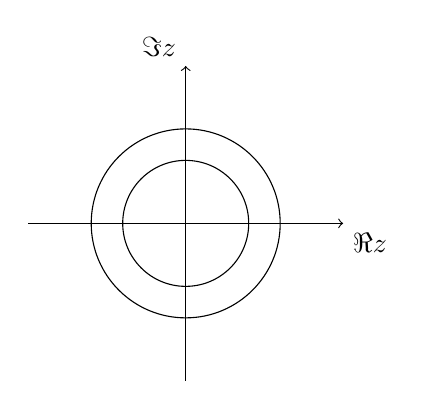
\begin{tikzpicture}[scale=1]
		\draw[->] (-2,0) -- (2,0) node[anchor=north west] {$\Re{z}$};
		\draw[->] (0,-2) -- (0,2) node[anchor=south east] {$\Im{z}$};
		\clip (-2,-2) rectangle (2,2);
		\draw (0,0) circle (1.2cm);
		\draw (0,0) circle (0.8cm);
		\end{tikzpicture}
	\end{center}
	Se per assurdo la serie converge in $z\Rightarrow$ per il teorema precedente  avremmo convergenza in ogni sfera con raggio minore di $\abs{\frac{1}{z}}$. e quindi anche in $w$ questo nega l'ipotesi.ASSURDO.
\end{proof}
\observation
Come è fatto l'insieme su cui si ha convergenza??\\
segue da queste due ultime proposizioni che se $\left\{a_n:n\in\N\right\}$ è una successione in $\C$ allora l'insieme $\left\{z\in\C:\sum\limits_{n=0}^{+\infty}a_nz^n converge\right\}$ è un cerchio.\\Sulla circonferenza non ci soffermaiamo a capire cosa accade poiché tutto può accadere.
\definition
Raggio di convergenza della serie $\sum\limits_{n=0}^{+\infty}a_nz^n\bydef \rho=\sup\left\{r\ge 0 :\sum\limits_{n=0}^{+\infty}a_nz^n converge su B(0,r)\right\}$
\observation
Il raggio di convergenza di una serie di potenze può essere $0$, un numero reale positivo o $+\infty$.
\observation
una definizione come $\rho=\inf\left\{r\ge 0 :\sum\limits_{n=0}^{+\infty}a_nz^n non converge su B(0,r)\right\}$ non sta in piedi poiché questo insieme potrebbe essere vuoto, mentre quello sopra non è mai vuoto, poerché $r=0$ c'è sempre poiché in $0$ si ha sempre convergenza. Ilsecondo potrebbe essere vuoto perché ci sono serie che convergono su tuttoil piano complesso e quindi non si avrebbe nessun $r$ fuori da quale non sia ha convergenza.\\
\proposition CRITERIO DELLA RADICE.\\
Data la serie di potenze $\sum\limits_{n=0}^{+\infty}a_nz^n$, sia $l=\lim\limits_{n\to+\infty}\sqrt[n]{\abs{a_n}}$.\\
Se questo limite esiste, allora il raggio di convergenza è
$\rho =
	\begin{cases}
		0				&	\text{se }l=+\infty\\
		\frac{1}{l} 	&	\text{se }l\in\left]0,+\infty\right[\\
		+\infty 		& 	\text{se }l=0
	\end{cases}
$
\proposition CRITERIO DEL RAPPORTO.\\
Data la serie di potenze $\sum\limits_{n=0}^{+\infty}a_nz^n$, sia $l=\lim\limits_{n\to+\infty}\frac{a_{n+1}}{a_n}$.\\
Se questo limite esiste, allora il raggio di convergenza è
$\rho =
\begin{cases}
0				&	\text{se }l=+\infty\\
\frac{1}{l} 	&	\text{se }l\in\left]0,+\infty\right[\\
+\infty 		& 	\text{se }l=0
\end{cases}
$
ESEMPIO::$e^z=\sum\limits_{n=0}^{+\infty}\frac{1}{n!}z^n$\\
$a_n=\frac{1}{n!} ...  \abs{\frac{a_{n+1}}{a_n}}=\frac{\frac{1}{(n+1)!}}{\frac{1}{n!}}=\frac{n!}{(n+1)!}=\frac{1}{n+1}\overset{n\to+\infty}{\to}0 \Rightarrow \rho=+\infty$\\
ESEMPIO::$sin(z)=\sum\limits_{n=0}^{+\infty}\frac{(-1)^nz^{2n+1}}{(2n+1)!}$ quindi
$a_n =
\begin{cases}
0		&	\text{se }n\text{ è pari}\\
...		&	\text{se }n\text{ è dispari}\\
\end{cases}
$\\
...\\
...\\
...\\
ESEMPIO::$sin(z)=\sum\limits_{n=0}^{+\infty}\frac{(-1)^nz^{2n}}{(2n)!}$ quindi
$a_n =
\begin{cases}
...		&	\text{se }n\text{ è pari}\\
0		&	\text{se }n\text{ è dispari}\\
\end{cases}
$\\
...\\
...\\
...\\
ESEMPIO:: $e^{iy}$ con $y\in \R$
$$e^{iy} = \sum\limits_{n=0}^{+\infty}\frac{1}{n!}(iy)^n = \sum\limits_{n=0}^{+\infty}\frac{1}{(2n)!}(iy)^{2n} + \sum\limits_{n=0}^{+\infty}\frac{1}{(2n+1)!}(iy)^{2n+1} = $$
$$ = \sum\limits_{n=0}^{+\infty}\frac{(-1)^n}{(2n)!}(y)^{2n} + i\sum\limits_{n=0}^{+\infty}\frac{(-1)^n}{(2n+1)!}(y)^{2n+1} = cos(y)+isin(y)$$
\begin{enumerate}
	\item $i^{2n}=\left(i^2\right)^n=(-1)^n$
	\item $i^{2n+1}=i\left(i^2\right)^n=i(-1)^n$
\end{enumerate}
ESEMPIO:: $e^{i\pi}+1=cos(\pi)+i\cdot sin(\pi)=0$\\
ESEMPIO:: $\sum\limits_{n=0}^{+\infty}z^n=\frac{1}{1-z}$ con $\rho=1$
ESEMPIO:: Sia $f(x)=\frac{1}{1+x^2}=\frac{1}{1-(-x^2)} = \sum\limits_{n=0}^{+\infty}(-x^2)^n=\sum\limits_{n=0}^{+\infty}(-1)^nx^{2n}$\\
QUI GRAFICO ..............\\
..........................\\
Questa serieconverge esclusivamente per $\abs{x}<1$, mentre la funzione $f$ è definita su tutto $ \R$, $f\in \cntclass{\infty}( \R; \R)$\\
In $\C$, lafunzione $f(z)=\frac{1}{1+z^2}$ è la somma della serie $\sum\limits_{n=0}^{+\infty}(-1)^nz^{2n}$ che ha raggio di convergenza  $\rho=1$. Infatti, $f(z)$ è singolare sia in $z=i$ sia in $z=-i$.\\
ALTRO GRAFICO::::::::::::::::\\
................................\\

\subsection{Serie di Taylor}
ESEMPIO:: $ln(1+z)$. Calcolare la Serie di Taylor.\\
$$D\left[ln(1+z)\right] = \frac{1}{1+z} = \sum\limits_{n=0}^{+\infty}(-1)^nz^n$$
$$\int \sum\limits_{n=0}^{+\infty}(-1)^nz^n dz = \sum\limits_{n=0}^{+\infty}\frac{(-1)^n}{n+1}z^{n+1}=\sum\limits_{n=1}^{+\infty}\frac{(-1)^{n-1}}{n}z^n$$
\begin{lemma}
	\label{lemma:taylor_rad_convergency}
	Sia $\brackets{a_n:n \in \N}$ una successione a valori in $\C$. Le serie:
	$$\sum_{n=0}^{+\infty} a_n z^n ,\qquad \sum_{n=1}^{+\infty} n a_n z^{n-1} \qquad\text{e}\qquad \sum_{n=0}^{+\infty} \frac{a_n}{n+1}z^{n+1}$$
	hanno lo stesso raggio di convergenza
	\begin{proof}
		Omessa
	\end{proof}
\end{lemma}

\definition
Sia $r\in \R$ con $r>0$. La funzione $f$ si dice analitica su $\left]-r,r\right[ \bydef f(x)=\sum\limits_{n=0}^{+\infty}a_nx^n \quad \forall x\in\left]-r,r\right[$ per opportuni $a_n\in \R$
\observation
In altre parole chiamiamo analitica una funzione che può essere scritta come somma di una serie di potenze convergente su $\left]-r,r\right[$ \\
ESEMPIO:: $x\to e^x$ è analitica su $ \R$\\
ESEMPIO:: $x\to\frac{1}{1+x^2}$ è analitica su $\left]-1,1\right[$\\
\proposition
Se $f$ è analitica su $\left]-r;r\right[$ per $r\in \R$ e $r>0\Rightarrow f\in \cntclass{0}(\left]-r,r\right[; \R)$
\begin{proof}
	$f$ è analitica  allora posso scriverla come $f=\sum\limits_{n=0}^{+\infty}a_nx^n$ cioè la funzione è limite di una serie, se la serie converge totalmente allora converge uniformemente. Il limite uniforme di funzioni continue(in questo caso polinomi) è una funzione continua. cioè la $f$ è continua.
\end{proof}
\proposition PROP+PROOF\\
Sia $f:\left]-r,r\right[\to \R$ e $f$ analitica su $\left]-r,r\right[ \bydef f(x)=\sum\limits_{n=0}^{+\infty}a_nx^n \Rightarrow$ ho convergenza totale $\Rightarrow$ ho convergenza uniforme di funzioni continue
$$\Rightarrow f\in \cntclass{0}(\left]-r,r\right[; \R),\quad a_0=f(0)$$
La serie delle derivate $\sum\limits_{n=0}^{+\infty}na_nx^{n-1}$ converge totalmente su $\left]-r,r\right[$ cioè
$$\sum\limits_{n=0}^{+\infty}f'(x)=\sum\limits_{n=0}^{+\infty}na_nx^{n-1} \uconvarrow g$$
$$\sum\limits_{n=0}^{+\infty}fn(0)\to f(0), f_n\in ????????????$$
Allora la serie delle derivate converge alla derivata della serie
$$\Rightarrow \in \cntclass{1}(\left]-r,r\right[; \R),\quad a_1=f'(0)$$
Questo ragionmento può essere ripetuto:
$$\Rightarrow \forall k\in\N,\quad f\in \cntclass{k}(\left]-r,+r\right[),\quad a_k=k!f^{(k)}(0)$$
e analogamente
$$f\in \cntclass{\infty}(\left]-r,r\right[; \R),\quad f(x)=\sum\limits_{n=0}^{+\infty}\frac{1}{n!}f^{(n)}(0)x^n$$
\observation Qui abbiamo detto se $f$ è analitica $\Rightarrow \ldots$, vorrei fare un qualche tipo di viceversa per poter capire se $f$ è analitica o no.
\proposition
Sia $f:\left]-r,r\right[\to \R$
\begin{center}
	$\left.\begin{matrix}
	f\in \cntclass{\infty}(\left]-r,r\right[; \R)\\
	\sum\limits_{n=0}^{+\infty}\frac{1}{n!}f^{(n)}(0)x^n\text{ converge totalmente su } \left]-r,r\right[\\
	\end{matrix}\right\}\Rightarrow f$ è analitica  .....
\end{center}
Per avere $f$ analitica  necessariamente come ipotesi deve esserci $f\in \cntclass{\infty}$ e $f$ che si può scrivere come sviluppo in serie di Taylor,dalla proposizione precedente. Questo basta? NO\\
ESEMPIO:: $f(x)=\left\{\begin{matrix}0&& x=0\\e^{-\frac{1}{x^2}}&&x\ne 0\end{matrix}\right.$\\
\begin{center}
	\begin{tikzpicture}[scale=1]
	%\draw[->] (0,-4) -- (0,4) node[anchor=north west] {$x$};
	%\draw[->] (-0.1,0) -- (1.2,0) node[anchor=south east] {$y$};
	%\clip (-4,0) rectangle (4,1);
	%\draw[domain=-4:4,smooth,variable=\x] plot ({\x},{{-1/(\x*\x)}});
	\end{tikzpicture}
\end{center}
\begin{enumerate}
	\item $f\in \cntclass{\infty}( \R; \R)$
	\item $\sum\limits_{n=0}^{+\infty}\frac{1}{n!}f^{(n)}(0)x^n$ converge totalmente su $ \R$
	\item $f(x)\ne\sum\limits_{n=0}^{+\infty}\frac{1}{n!}f^{(n)}(0)x^n$
\end{enumerate}
\begin{enumerate}
	\item Vediamo se è $\cntclass{0}$, quindi calcolo $\lim\limits_{x\to 0^{+}}f(x)=\lim\limits_{x\to 0^{-}}f(x)=0=f(0)\Rightarrow f\in \cntclass{0}( \R; \R)$.\\
	Ora calcoliamo la derivata fuori dallo zero, ne facciamo il limite per $x\to 0$ da destra e da sinitra e vediamo cosa succede.\\
	Se $x\ne 0$, $f'(x)=\frac{2}{x^3}e^{-\frac{1}{x^3}}$ e $\lim\limits_{x\to 0^{+}}f'(x)=\lim\limits_{x\to 0^{-}} = 0\Rightarrow f\in \cntclass{1}( \R; \R)$\\
	..........\\
	ancora una derivata.......\\
	..........\\
	Continuando a derivare  avremmo sempre un rapporto di polinomi che moltiplica un esponenziale, e l'esponenziale vince sempre. quindi fa $0$.
	itero il ragionamento......\\
	.......\\
	\item In (1) abbiamo visto  che tutte le derivate nello zero si annullavano, cioè
	$$\forall n\in\N, f^{(n)}(0)=0\Rightarrow \sum\limits_{n=0}^{+\infty}\frac{1}{n!}f^{(n)}(0)x^n$$
	è la serie identicamente nulla  che banalmente converge totalmente su tutto $ \R$
	\item Anche osservandoil grafico è chiaro che la $f$ non è la funzione identicamente nulla cioè è diversa dal suo sviluppo in serie
	$$f(x)\ne\sum\limits_{n=0}^{+\infty}\frac{1}{n!}f^{(n)}(0)x^n$$
\end{enumerate}
Il Problema nasce dall'$o(x^n)$ che scriviamo alla fine dello sviluppo n-esimo di questa funzione, perché l'intorno in cui si ha $o(x^n)$ diventa sempre più piccolo.
GRAFICO...\\
GRAFICO...\\
Mandando l'ordine $n$ all'infinito, l'intervallo su cui si ha l'o piccolo tende a diventare un punto (lo zero). Quindi abbiamo l'ugualianza tra la funzione e il suo sviluppo solo nell'origine.????????NON COMPRESA????\\
????????NON COMPRESA????\\
????????NON COMPRESA????\\
????????NON COMPRESA????\\
Completiamo le ipotesi con la prossima proposizione:
\proposition
Sia $f:\left]-r,r\right[\to \R$
\begin{center}
	$\left.\begin{matrix}
	f\in \cntclass{\infty}(\left]-r,r\right[; \R)\\
	\exists H,K >0 :\forall n\in\N \sup\limits_{\left]-r,r\right[}\abs{f^{(n)}(x)}\le HK^n\\
	\end{matrix}\right\}
	\Rightarrow f(x)=\sum\limits_{n=0}^{+\infty}\frac{1}{n!}f^{(n)}(0)x^n$
\end{center}
\observation
L'ipotesi centrale ............. qui non c'è
\observation
Sia $\sum\limits_{n=0}^{+\infty}(z,w)^n$ una serie di potenze in due variabili.\\
Quando abbiamo due variabili, non si può parlare di raggio di convergenza. Questa serie è una serie geometrica che converge sse $\abs{zw}<1$. è  difficile parlare di raggio di convergenza  perché essendo $z,w\in\C$, se per una variabile servono due dimensioni per due variabili servono quattro dimensioni , e anche se non riusciamo a fare il disegno è evidente che l'insieme su cui la serie converge non è un cerchio(sfera).
\begin{example}[Esempi di Sviluppi in serie di Taylor]
	\label{ex:tay_series_examples}
	\begin{description}
		\item $e^x=\sum\limits_{n=0}^{+\infty}\frac{1}{n!}x^n$
		\item $sin(x)=\sum\limits_{n=0}^{+\infty}\frac{(-1)^n}{(2n+1)!}x^{(2n+1)}$
		\item $sinh(x)=\sum\limits_{n=0}^{+\infty}\frac{1}{(2n+1)!}x^{(2n+1)}$
		\item $cos(x)=\sum\limits_{n=0}^{+\infty}\frac{(-1)^n}{(2n)!}x^{(2n)}$
		\item $cosh(x)=\sum\limits_{n=0}^{+\infty}\frac{1}{(2n)!}x^{(2n)}$
		\item $\frac{1}{1-x}=\sum\limits_{n=0}^{+\infty}x^n$
		\item $ln(1+x)=\sum\limits_{n=1}^{+\infty}\frac{(-1)^{n+1}}{n}x^n$
		\item $arctan(1+x)=\sum\limits_{n=0}^{+\infty}\frac{(-1)^{n}}{2n+1}x^{(2n+1)}$
		\item $\frac{1}{1+x^2}=\sum\limits_{n=0}^{+\infty}(-1)^nx^2n$
		\item $\sum\limits_{n=0}^{+\infty}\frac{1}{n^\lambda}=\left\{\begin{matrix}\text{converge sse } \lambda >1\\ \text{diverge sse } \lambda \le 1 \end{matrix}\right.$
		\item $\sum\limits_{n=0}^{+\infty}q^n=\left\{\begin{matrix}\text{converge sse } \abs{q}<1, S=\frac{1}{1-x}\\ \text{diverge sse } \abs{q}>1\text{ o }q=1\\\nexists \text{ sse } x=-1 \end{matrix}\right.$
	\end{description}
\end{example}
\begin{exercise}
	\label{ex:deriv_func_with_taylor}
	Determinare le derivate delle funzioni
	\begin{itemize}
		\vspace*{-4ex} % I've no idea WTF is wrong with these equations, but the spacing is atrocious without this ugly fix
		\item $x \to \sin x$
		\vspace*{-5ex}
		\item $x \to \cos x$
		\vspace*{-5ex}
		\item $x \to e^x$
		\vspace*{-4ex}
	\end{itemize}
	utilizzando \fullref{ex:tay_series_examples}, il \fullref{lemma:taylor_rad_convergency} ed il \fullref{coro:deriv_series_series_of_deriv}.
\end{exercise}

\subsection{Serie di Fourier}
\definition
Siano $A\subseteq \R$, $f:A\to \R$ e $T>0$, $f$ è $T$-periodica $\bydef \forall x\in A
\left\{\begin{matrix}
x+T\in A\\f(x+T)=f(x)
\end{matrix}\right. $\\


ESEMPIO:: $\lfloor x \rfloor = \text{ parte intera } = \max\left\{k\in\mathbb{Z}:k\le x\right\}$
$$\lfloor \pi \rfloor=3, \quad \lfloor \sqrt{2} \rfloor = 1 \quad \lfloor -e \rfloor = -3 $$
\begin{center}
	\begin{tikzpicture}
		\draw[->] (-4,0) -- (4,0) node[anchor=north west] {$x$};
		\draw[->] (0,-4) -- (0,4) node[anchor=south east] {$y$};

		\foreach \num in {-3,...,3} {
			\draw[line width=0.25mm] (\num , \num) -- (\num+1 , \num);
			\draw[fill=black] (\num , \num) circle (0.1cm);
			\draw (\num+1, \num) circle (0.1cm);
		}
	\end{tikzpicture}
\end{center}
è $1$-periodica.
ESEMPIO:: $mant(x)=\text{ mantissa di x } = x- \lfloor x \rfloor$
\begin{center}
	\begin{tikzpicture}
	\draw[->] (-4,0) -- (4,0) node[anchor=north west] {$x$};
	\draw[->] (0,-4) -- (0,4) node[anchor=south east] {$y$};

	\foreach \num in {-3,...,3} {
		\draw[line width=0.25mm] (\num , 0) -- (\num+1 , 1);
		\draw[fill=black] (\num , 0) circle (0.1cm);
		\draw (\num+1, 1) circle (0.1cm);
	}
	\end{tikzpicture}
\end{center}
è $1$-periodica.
\observation
La funzione costante è $T$-periodica $\forall T>0$, ma non ha un periodo minimo, per questo motivo non la consideriamo.
\observation
Sia $f:A\to \R$ $T$-periodica. Allora possiamo definire $\overline{f}:\overline{A}\to \R$ che sia $2\pi$-periodica data da:
$$x\to f\left(\frac{T}{2\pi}x\right),\quad \overline{A}=\frac{2\pi}{T}A$$
\proposition
Siano $A\subseteq \R$, $f:A\to \R$ e $T>0$\\
$f$ è $T$-periodica $\Rightarrow \forall n\in\N$, $f$ è $nT$-periodica.
\proposition
Sia $f:\left[0,2\pi\right[\to \R \Rightarrow \exists ! \hat{f}: \R\to \R$ t.c.: $\left\{\begin{matrix} \hat{f} 2\pi-periodica\\\hat{f}_{\left|\left[0,2\pi\right]\right.}=f\end{matrix}\right.$
\begin{proof}
	$\forall x\in \R. \exists ! \hat{x}\in\left[0,2\pi\right[$ t.c.: $x=2\pi\cdot k+\hat{x}$ con $k\in\mathbb{Z}$ e $k=\left[??????\right]$\\
	$$\hat{f}(x)=f(\hat{x})$$
\end{proof}
cioè se noi estendiamo una funzione definita su $\left[0,2\pi\right[$ a tutto $ \R$ otteniamo una funzione unica e periodica.
\observation
Con i polinomi di Taylor ........\\
........\\
........\\
........\\
........\\
........\\
\definition
Dati $2n+1$ numeri reali $a_0,a_1,\dotsc,a_n,b_1,\dotsc,b_n$ si dice polinomio trigonometrico di coefficienti $a_0,a_1,\dotsc,a_n,b_1,\dotsc,b_n$ la funzione:
$$\begin{array}{rcl} p: \left[-\pi,\pi\right] & \to &  \R \\ x & \to & \frac{a_0}{2}+\sum\limits_{k=1}^{N}\left(a_ncos(nx)+b_nsin(nx)\right) \end{array}$$
\observation
Essendo un'approssimazione, si deve aggiungere l'errore. Come è fatto?. Per far uscire conti giusti e comodi andrebbe usata la distanza quadratica , ma questo prevede una lunga parte introduttiva, noi allora lo stimiamo con la distanza infinita.
\definition
Date due successioni di numeri reali $\left\{a_n:n\in\N\right\}$,$\left\{b_n:n\in\N\setminus\left\{0\right\}\right\}$, si defininisce serie trigonometrica di coefficienti  $\left\{a_n:n\in\N\right\}$,$\left\{b_n:n\in\N\setminus\left\{0\right\}\right\}$ la serie
$$\begin{array}{rcl} \mathfrak{F}: \left[-\pi,\pi\right] & \to &  \R \\ x & \to & \frac{a_0}{2}+\sum\limits_{k=1}^{+\infty}\left(a_ncos(nx)+b_nsin(nx)\right) \end{array}$$
LEMMA::\\
Se $h,k\in\N$ valgono le seguenti uguaglianze:
\begin{description}
	\item[$\ast$]
	$\int_{-\pi}^{\pi} cos(hx)cos(kx)=
	\left\{\begin{matrix}
	0 &&h\ne k\\\pi&&0\ne h=k\\2\pi&&0=h=k
	\end{matrix}\right.$
	\item[$\ast$] $\int_{-\pi}^{\pi}cos(hx)sin(kx)= 0 $
	\item[$\ast$]
	$\int_{-\pi}^{\pi}sin(hx)sin(kx)=
	\left\{\begin{matrix}
	0 &&h\ne k\text{ oppure }h=k=0\\ \pi&&0\ne h=k
	\end{matrix}\right.$
\end{description}
ESERCIZIO:: IL POLINOMIO DI FOURIER FORNISCE LA MIGLIORE APPROSSIMAZIONE NEL SENSO DELLA DISTANZA QUADRATICA.\\
Sia $f: \realintervalclose{-\pi}{\pi} \mapsto \R$, quale è la funzione a lei più vicina nel senso della distanza quadratica?\\
Fisso $N\in\N$ e prendo il polinomio trigonometrico di grado $N$
$$p_N(x)=\trigonpol{n}{1}{N}$$
con $a_0,a_1,\dotsc,a_n,b_1,\dotsc,b_n\in \R$, il problema è quello di minimizzare $d_2(f,p_n)$ quindi un problema di minimo. Stiamo cercando i coefficienti del polinomio trigonometrico quindi studiamo una funzione $\varphi(a_0,a_1,\dotsc,a_N,b_1,\dotsc,b_N) = \sqrt{\int_{-\pi}^{\pi}\left[f(x)-p_n(x)\right]^2}\integrald{x}$.\\
Essendo la funzione radice quadrata monotona crescente ne studiamo solo il radicando:
$$\varphi(a_0,a_1,\dotsc,a_N,b_1,\dotsc,b_N)=\int_{-\pi}^{\pi}\left[\trigonpol{n}{1}{N}-f(x)\right]^2dx$$
\observation
con $f\in \cntclass{1}$:
$$F(\alpha,\beta,x)=\int_{\alpha}^{\beta}f(x,t)\integrald{t}$$
$$\partial_\alpha F(\alpha,\beta,x)=-f(x,\alpha)\integrald{t}$$
$$\partial_\beta F(\alpha,\beta,x)=f(x,\beta)\integrald{t}$$
$$\nabla_x F(\alpha,\beta,x)=\int_{\alpha}^{\beta}\nabla_xf(x,t)\integrald{t}$$
Qudindi applicando al nostro caso otteniamo
$$\partial_{a_0}\varphi = \int_{-\pi}^{\pi}\partial_{a_0}\left(\left[\trigonpol{n}{1}{N}-f(x)\right]^2\right)\integrald{x}=$$
$$ = \int_{-\pi}^{\pi} \frac{1}{2}2\left(\trigonpol{n}{1}{N}-f(x)\right)\integrald{x}=$$
$$ =  \int_{-\pi}^{\pi} \frac{a_0}{2}\integrald{x} + $$
$$\int_{-\pi}^{\pi} a_1cos(x)\integrald{x} +
\ldots +
\int_{-\pi}^{\pi} a_Ncos(Nx)\integrald{x} + $$
$$\int_{-\pi}^{\pi} b_1sin(x)\integrald{x} +
\ldots +
\int_{-\pi}^{\pi} b_Nsin(Nx)\integrald{x} - $$
$$ \int_{-\pi}^{\pi} f(x)\integrald{x} = $$
L'integrale di una sinusoide su un multiplo intero del periodo è $0$ quindi
$$=\pi a_0-\int_{-\pi}^{\pi}f(x)\integrald{x}$$
Calcolando direttamente anche le derivate seconde si ottiene che
$$\partial^2_{a_0a_0}=\pi\quad\partial^2_{a_0a_n}=0\quad\partial^2_{a_0b_n}=0\quad\forall n=1,\dotsc,N$$

$$\partial_{a_k}\varphi = \int_{-\pi}^{\pi}\partial_{a_k}\left(\left[\trigonpol{n}{1}{N}-f(x)\right]^2\right)\integrald{x}=$$
$$ = \int_{-\pi}^{\pi} 2cos(kx) \left[\trigonpol{n}{1}{N}-f(x)\right]\integrald{x}=$$
$$ =  \cancel{\int_{-\pi}^{\pi} a_0cos(kx)\integrald{x}} + $$
$$\cancel{\int_{-\pi}^{\pi} 2a_1cos(x)cos(kx)\integrald{x}} +
\ldots +
\int_{-\pi}^{\pi} 2a_kcos(kx)cos(kx)\integrald{x}
\ldots +
\cancel{\int_{-\pi}^{\pi} 2a_Ncos(Nx)cos(kx)\integrald{x}} + $$
$$\cancel{\int_{-\pi}^{\pi} 2b_1sin(x)cos(kx)\integrald{x}} +
\ldots +
\cancel{\int_{-\pi}^{\pi} 2b_ksin(kx)cos(kx)}\integrald{x}
\ldots +
\cancel{\int_{-\pi}^{\pi} 2b_Nsin(Nx)cos(kx)\integrald{x}} - $$
$$\int_{-\pi}^{\pi} 2f(x)cos(kx)\integrald{x} = $$
E anche applicando il lemma
$$=2\pi\left[a_k-\int_{-\pi}^{\pi}f(x)cos(kx)\integrald{x}\right]$$
Calcolando direttamente anche le derivate seconde si ottiene che
$$\partial^2_{a_ka_0}=\pi\quad\partial^2_{a_ka_n}=
\left\{\begin{matrix}
0&&n\ne k\\2\pi&&n=k
\end{matrix}\right.
\quad\partial^2_{a_kb_n}=0\quad\forall n=1,\dotsc,N$$

$$\partial_{b_k}\varphi = \int_{-\pi}^{\pi}\partial_{b_k}\left(\left[\trigonpol{n}{1}{N}-f(x)\right]^2\right)\integrald{x}=$$
$$ = \int_{-\pi}^{\pi} 2sin(kx) \left[\trigonpol{n}{1}{N}-f(x)\right]\integrald{x}=$$
$$ =  \cancel{\int_{-\pi}^{\pi} a_0sin(kx)\integrald{x}} + $$
$$\cancel{\int_{-\pi}^{\pi} 2a_1cos(x)sin(kx)\integrald{x}} +
\ldots +
\cancel{\int_{-\pi}^{\pi} 2a_kcos(kx)sin(kx)}\integrald{x}
\ldots +
\cancel{\int_{-\pi}^{\pi} 2a_Ncos(Nx)sin(kx)\integrald{x}} + $$
$$\cancel{\int_{-\pi}^{\pi} 2b_1sin(x)sin(kx)\integrald{x}} +
\ldots +
\int_{-\pi}^{\pi} 2b_ksin(kx)sin(kx)\integrald{x}
\ldots +
\cancel{\int_{-\pi}^{\pi} 2b_Nsin(Nx)sin(kx)\integrald{x}} - $$
$$\int_{-\pi}^{\pi} 2f(x)sin(kx)\integrald{x} = $$
E anche applicando il lemma
$$=2\pi\left[b_k-\int_{-\pi}^{\pi}f(x)cos(kx)\integrald{x}\right]$$
Calcolando direttamente anche le derivate seconde si ottiene che
$$\partial^2_{b_ka_0}=\pi\quad\partial^2_{b_ka_n}=
\left\{\begin{matrix}
0&&n\ne k\\2\pi&&n=k
\end{matrix}\right.
\quad\partial^2_{b_kb_n}=0\quad\forall n=1,\dotsc,N$$
Si verifica la condizione $\nabla\varphi = 0$ con
\begin{description}
	\item[$\ast$] $a_0=\frac{1}{\pi}\int_{-\pi}^{\pi}f(x)\integrald{x}$
	\item[$\ast$] $a_k=\frac{1}{\pi}\int_{-\pi}^{\pi}f(x)cos(kx)\integrald{x}$
	\item[$\ast$] $b_k=\frac{1}{\pi}\int_{-\pi}^{\pi}f(x)sin(kx)\integrald{x}$
\end{description}
La matrice Hessiana di $\varphi$ risulta $$H_{\varphi}=\left[\begin{matrix}
\pi&&0&&0&&\ldots&&0\\
0&&2\pi&&0&&\ldots&&0\\
0&&0&&2\pi&&\ldots&&0\\
\vdots&&\vdots&&\vdots&&\ddots&&\vdots\\
0&&0&&0&&0\ldots&&2\pi
\end{matrix}\right]$$
è una matrice diagonale quindi si leggono direttamente tutti gli autovalori che sono strettamente positivi quindi la forma quadratica è definita positiva ed il punto in questione è un punto di minimo assoluto.
\definition
Sia $f: \realintervalclose{-\pi}{\pi} \mapsto \R$, i coefficienti di Fourier di $f$ sono (ovviamente $f$ deve essere tale da ammetterli finiti):
$$a_0=\frac{1}{\pi}\int_{-\pi}^{\pi}f(x)\integrald{x}$$
$$a_k=\frac{1}{\pi}\int_{-\pi}^{\pi}f(x)cos(kx)\integrald{x}\quad k\in\N\setminus{\left\{0\right\}}$$
$$b_k=\frac{1}{\pi}\int_{-\pi}^{\pi}f(x)sin(kx)\integrald{x}\quad k\in\N\setminus{\left\{0\right\}}$$
La serie di Fourier di $f$ è
$$\trigonpol{k}{1}{+\infty}$$
\proposition
Sia $F: \realintervalclose{-\pi}{\pi} \mapsto \R$ la somma della serie trigono metrica definita dai coefficienti $\left\{a_n:n\in\N\right\}$ e $\left\{a_n:n\in\N\setminus{\left\{0\right\}}\right\}$ e la serie trigonometrica converge uniformemente allora $F$ è una funzione continua e
$$a_k=\frac{1}{\pi}\int_{-\pi}^{\pi}F(x)cos(kx)\integrald{x}\quad k\in\N$$
$$b_k=\frac{1}{\pi}\int_{-\pi}^{\pi}F(x)sin(kx)\integrald{x}\quad k\in\N\setminus{\left\{0\right\}}$$
ESEMPIO+DIMOSTRAZIONE:::\\
sia $f(x)=\trigonpol{n}{1}{+\infty}$. Allora:\\
$$a_0=\frac{1}{\pi}\int_{-\pi}^{\pi}f(x)\integrald{x}=\frac{1}{\pi}\int_{-\pi}^{\pi}\trigonpol{n}{1}{+\infty}\integrald{x}=$$
$$
= \frac{1}{\pi}\int_{-\pi}^{\pi}\frac{a_0}{2} +
\frac{1}{\pi}\int_{-\pi}^{\pi}\left(\sum\limits_{n=1}^{+\infty} a_ncos(nx)\right)\integrald{x} +
\frac{1}{\pi}\int_{-\pi}^{\pi}\left(\sum\limits_{n=1}^{+\infty} b_ncos(nx)\right)\integrald{x}
$$
Poiché si ha convergenza uniforme si può portare l'integrale dentro la sommatoria.
$$
= \frac{1}{\pi}\int_{-\pi}^{\pi}\frac{a_0}{2} +
\cancel{\frac{1}{\pi}\sum\limits_{n=1}^{+\infty}\int_{-\pi}^{\pi} a_ncos(nx)\integrald{x}} +
\cancel{\frac{1}{\pi}\sum\limits_{n=1}^{+\infty}\int_{-\pi}^{\pi} b_ncos(nx)\integrald{x}}=
$$
$$=\frac{1}{\pi}\frac{a_0}{2}\left(\pi-(-\pi)\right)=a_0$$


$$a_k=\frac{1}{\pi}\int_{-\pi}^{\pi}f(x)cos(kx)\integrald{x}=$$
$$\frac{1}{\pi}\left[
\cancel{\int_{-\pi}^{\pi}\frac{a_0}{2}cos(kx)\integrald{x}}+
\int_{-\pi}^{\pi}\left(\sum\limits_{n=1}^{+\infty}a_ncos(nx)cos(kx)\right)\integrald{x}+
\cancel{\int_{-\pi}^{\pi}\left(\sum\limits_{n=1}^{+\infty}b_nsin(nx)cos(kx)\right)\integrald{x}}
\right]=$$
$$\frac{1}{\pi}\left[
\cancel{\int_{-\pi}^{\pi}\left(\sum\limits_{n=1}^{k-1} a_ncos(nx)cos(kx)\right)\integrald{x}}+
\int_{-\pi}^{\pi}a_kcos(kx)cos(kx)\integrald{x}+
\cancel{\int_{-\pi}^{\pi}\left(\sum\limits_{n=k+1}^{+\infty}a_ncos(nx)cos(kx)\right)}\integrald{x}
\right]=$$
$$=\frac{1}{\pi}\pi a_k=a_k$$

$$b_k=\frac{1}{\pi}\int_{-\pi}^{\pi}f(x)sin(kx)\integrald{x}=$$
$$\frac{1}{\pi}\left[
\cancel{\int_{-\pi}^{\pi}\frac{a_0}{2}sin(kx)\integrald{x}}+
\int_{-\pi}^{\pi}\left(\sum\limits_{n=1}^{+\infty}a_ncos(nx)sin(kx)\right)\integrald{x}+
\cancel{\int_{-\pi}^{\pi}\left(\sum\limits_{n=1}^{+\infty}b_nsin(nx)sin(kx)\right)\integrald{x}}
\right]=$$
$$\frac{1}{\pi}\left[
\cancel{\int_{-\pi}^{\pi}\left(\sum\limits_{n=1}^{k-1} a_ncos(nx)sin(kx)\right)\integrald{x}}+
\int_{-\pi}^{\pi}a_kcos(kx)sin(kx)\integrald{x}+
\cancel{\int_{-\pi}^{\pi}\left(\sum\limits_{n=k+1}^{+\infty}a_ncos(nx)sin(kx)\right)}\integrald{x}
\right]=$$
$$=\frac{1}{\pi}\pi b_k=b_k$$
\observation
Se $d_2(f,\text{polinomio di Fourier})$ \`{e} minima $\Rightarrow$ il polinomio di Fourier \`{e} costruito con i coefficienti di Fourier di $f$.
\observation
Se $f$ \`{e} somma di una serie di funzioni $\Rightarrow$ i coefficienti della serie sono i coefficienti di Fourier.
\observation
Funzioni diverse possono avere gli stessi coefficienti di Fourier, cio\`{e} $\exists f,g$ con $f\ne g$ ma $f$ e $g$  hanno gli stessi coefficienti di Fourier.
ESEMPIO::
\begin{center}
	\begin{tikzpicture}
		\draw[->] (-2,0) -- (2,0) node [anchor=north west]{$x$};
		\draw[->] (0,0) -- (0,2);
		\clip (-2,0) rectangle (2,2);
		\draw[domain=-2:2,smooth,red,variable=\x] plot ({\x},{1}) node{$f$};
		\draw[domain=-2:2,smooth,blue,variable=\x] plot ({\x},{1}) node{$g$};
	\end{tikzpicture}
	SISTEMARE,
\end{center}
\observation
I coefficienti di Fourier non possono identificare univocamente puntualmente una funzione.
\subsubsection{Punto Di Vista Geometrico}
In $R^2$ Ci sono $2$ vettori $\hat{i},\hat{j}$ della base, se $\underline{v}\in \R^2 \Rightarrow \underline{v}=v_1\cdot \hat{i}+v_2\cdot \hat{j}$ con $v_1,v_2$ componenti di $\underline{v}$\\
Calcolo delle componenti:\\
$$\underline{v}\cdot \hat{i} = v_1\cdot \hat{i\cdot }\hat{i}+v_2\cdot \hat{j}\cdot \hat{i}=v_1$$
$$\underline{v}\cdot \hat{j} = v_1\cdot \hat{i}\cdot \hat{j}+v_2\cdot \hat{j}\cdot \hat{j}=v_2$$
Questo vale perché $\hat{i},\hat{j}$ è una base ortonormale.
In $R^3$ Ci sono $3$ vettori $\hat{i},\hat{j},\hat{k}$ della base, se $\underline{v}\in \R^3 \Rightarrow \underline{v}=v_1\hat{i}+v_2\hat{j}+v_3\hat{k}$ con $v_1,v_2,v_3$ componenti di $\underline{v}$\\
Calcolo delle componenti:
$$ v_1=\underline{v}\cdot \hat{i}\quad v_2=\underline{v}\cdot \hat{j}\quad v_3=\underline{v}\cdot \hat{k}  $$
In $R^n$ Ci sono $n$ vettori $e_1,e_2,\dotsc,e_n$ della base, se $\underline{v}\in \R^n \Rightarrow \underline{v}=v_1\cdot e_1+v_2\cdot e_2+\ldots+v_n\cdot e_n=\sum\limits_{k=1}^{n}v_k\cdot e_k$ con $v_1,v_2,\dotsc,v_n$ componenti di $\underline{v}$\\
Calcolo delle componenti:
$$v_k=\underline{v}\cdot e_k$$
\\
Con le Serie di Fourier su esegue la stessa operazione sullo spazi $\cntclass{0}(\realintervalclose{-\pi}{\pi}; \R)$. Come elementi di base si ha un insieme di funzioni:
\begin{enumerate}
	\item $c_0:x\to 1$
	\item $c_1:x\to cos(x)$
	\item $c_2:x\to cos(2x)$
	\item $\ldots$
	\item $c_n:x\to cos(nx)$
	\item $s_1:x\to sin(x)$
	\item $s_2:x\to sin(2x)$
	\item $\ldots$
	\item $s_n:x\to sin(nx)$
\end{enumerate}
Si possono osservare due cose:
\begin{enumerate}
	\item Sono tutte funzioni linearmente indipendenti, poiché l'unica combinazione lineare di questi elementi che da l'elemento nullo è quella a coefficenti tutti nulli.
\end{enumerate}
\definition
Il prodotto scalare in $\cntclass{0} \bydef \left<f,g\right>=\int_{-\pi}^{\pi}f(x)g(x)\integrald{x}$
Altre simbologie usate sono: $ f\bullet g $, $(f|g)$
\observation linearità\\
$$\left<(\alpha\cdot f+\beta\cdot g), h \right>= \int_{-\pi}^{pi} (\alpha\cdot f(x)+\beta\cdot g(x))\cdot h(x) \integrald{x}=$$
$$=\int_{-\pi}^{pi} \left[\alpha\cdot f(x)\cdot h(x)+\beta\cdot g(x)\cdot h(x) \right]\integrald{x}= $$
$$=\alpha\int_{-\pi}^{pi} \cdot f(x)\cdot h(x) \integrald{x}+\beta\int_{-\pi}^{pi} \cdot g(x)\cdot h(x) \integrald{x} =$$
$$\alpha\left<f,h\right>+\beta\left<g,h\right>$$

Ripetiamolo stesso ragionamento applicato in $ \R^2, \R^3,$ e $ \R^n$ per ricavare le componenti, possiamo fare questo perché abbiamo una base e abbiamo definito un prodotto scalare.\\
Se $f(x)=\trigonpol{n}{1}{+\infty} \Rightarrow $
$$a_0=\frac{1}{\pi}\int_{-\pi}^{\pi}f(x)dxs=\frac{1}{\pi}\left<f,c_0\right> $$
$$a_k=\frac{1}{\pi}\int_{-\pi}^{\pi}f(x)cos(kx)\integrald{x}=\frac{1}{\pi}\left<f,c_k\right> $$
$$b_k\frac{1}{\pi}\int_{-\pi}^{\pi}f(x)sin(kx)\integrald{x}=\frac{1}{\pi}\left<f,s_k\right>$$
Quindi come prima le componenti di un vettore si ottengono moltiplicando(prodotto scalare) il vettore per gli elementi della base.\\
PER IL LEMMA:\\
$$
\left<c_h,c_k\right>=
\left\{\begin{matrix}
0&&h\ne k\\
2\pi&&0=h=k\\
\pi&&0\ne h=k\\
\end{matrix}\right.
$$
$$ \left<c_h,s_k\right>=0$$
$$
\left<s_h,s_k\right>=
\left\{\begin{matrix}
0&&h\ne k\\
\pi&&0\ne h=k\\
\end{matrix}\right.
$$
Il prodotto scalare di elementi diversi è nullo quindi la base è ortogonale, ma non è ortonormale in quanto il prodotto scalare tra due elementi diversi della base non è unitario.(ecco perché gli $\frac{1}{\pi})$ e $\frac{a_0}{2}$)\\
In generale in geometria non è difficile normalizzare una base, è sufficiente dividere tutti gli elementi per la loro norma. In questo caso decidiamo di non applicare questo ragionamento poiché la norma vale $\sqrt{\pi}$ e se normalizziamo dobbiamo aggiungere questo termini ......\\
Il prodotto scalare in $\cntclass{0}$ è molto legato alla $d_2$ infatti:
$$\norm{f}_2=\sqrt{\left<f,f\right>}=\sqrt{\int_{-\pi}^{\pi}f(x)\cdot f(x)\integrald{x}}\sqrt{\int_{-\pi}^{\pi}\left[f(x)\right]^2dx}$$
Continuano le analogie:\\
In $ \R^2$ ........\\
In $ \R^3$ .........\\
.....\\
......\\
......\\
.....\\
Passando in dimensione infinita, abbiamo una funzione $f$ (come vettore $\underline{v}$) nello spazio, e fare il polinomio di Fourier  vuole dire proiettare la funzione $f$ in uno spazio fatto dai primi $2n+1$ elementi della base che è uno spazio di dimensione finita.\\
\\
Esempio:::: Non ogni funzione ammette coefficienti di Fourier finiti. La funzione
$$\begin{array}{rcl} f: \left[-\pi,\pi\right] & \to &  \R \\
x & \to & \left\{\begin{matrix} 0 && x=0\\\frac{1}{x^2}&&x\ne 0 \end{matrix}\right. \end{array}$$
non ammette coefficienti di Fourier finiti.\\
Esempio::: Una funzione può ammettere tutti i coefficienti di Fourier finiti ed una serie di Fourier convergente, ma ad un limite diverso da $f$.La funzione.
$$\begin{array}{rcl} f: \left[-\pi,\pi\right] & \to &  \R \\
x & \to & \left\{\begin{matrix} -1 && x<0\\1&&x>0 \end{matrix}\right. \end{array}$$
ha coefficienti di Fourier
$$a_k=0\quad\forall k,\quad\quad \left\{\begin{matrix}0 && k\text{ dispari }\\ \frac{4}{k\pi}&& k \text{ pari } \end{matrix}\right.$$
e serie di Fourier
$$ F_f(x)= \frac{4}{\pi}\sum\limits_{k=0}^{+\infty}\frac{sin(2h+1)x}{2h+1} $$
questa serie converge puntualmente in $0$ ma $F_f(0)\ne f(0)$\\

ESEMPIO:: Due funzioni diverse possono avere gli stessi coefficienti di Fourier:
$$\begin{array}{rcl} f: \left[-\pi,\pi\right] & \to &  \R \\
x & \to & \left\{\begin{matrix} -1 && x<0\\0&&x= 0\\1&&x>0 \end{matrix}\right.\end{array}$$
$$\begin{array}{rcl} g: \left[-\pi,\pi\right] & \to &  \R \\
x & \to & \left\{\begin{matrix} -1 && x<0\\\pi&&x= 0\\1&&x>0 \end{matrix}\right.\end{array}$$
\observation
Sia $f$ una funzione pari $\Rightarrow bn=0 \forall n=1,2,\dotsc,+\infty$
\observation
Sia $f$ una funzione dispari $\Rightarrow an=0 \forall n=0,1,,\dotsc,+\infty$
\observation
Siano
$$f(x)=\frac{a_0}{2}+\sum\limits_{n=}^{+\infty}\left(a_ncos(nx)+b_nsin(nx)\right)$$
$$\varphi(x)=\frac{\alpha_0}{2}+\sum\limits_{n=}^{+\infty}\left(\alpha_ncos(nx)+\beta_nsin(nx)\right)$$
Allora
$$ F(x)=(f+\varphi)(x)=\frac{A_0}{2}+\sum\limits_{n=}^{+\infty}\left(A_ncos(nx)+B_nsin(nx)\right)$$
con $A_n=a_n+\alpha_n$. $B_n=b_n+\beta_n$.
cioè i coefficienti di Fourier dipendono linearmente dalla funzione.\\
Esempio::: $B_3=\frac{1}{\pi}\int_{-\pi}^{\pi}F(x)sin(3x)\integrald{x}=\frac{1}{\pi}\int_{-\pi}^{\pi}(f(x)+\varphi(x))sin(3x)\integrald{x}=$\\
$\frac{1}{\pi}\left[\int_{-\pi}^{\pi}f(x)sin(3x)\integrald{x}+\int_{-\pi}^{\pi}\varphi(x)sin(3x)\integrald{x}\right]=b_3+\beta_3$\\
Sia $f(x)=\frac{a_0}{2}+\sum\liminf_{n=1}^{+\infty}\left(a_ncos(nx)+b_ncos(nx)\right)$ allora $F=4f=\frac{A_0}{2}+\sum\limits_{n=1}^{+\infty}\left(A_ncos(nx)+B_ncos(nx)\right)$ con $A_n=4a_n$, $B_n=4b_n$\\
ESEMPIO
Esempio:::$B_3=\frac{1}{\pi}\int_{-\pi}^{\pi}F(x)sin(3x)\integrald{x}=\frac{1}{\pi}\int_{-\pi}^{\pi}4f(x)sin(3x)\integrald{x}=4b_3$\\
\begin{definition}[Funzione Continua a Tratti]
	Siano $a,b\in \R$ con $a<b$, una funzione $f:\realintervalclose{a}{b} \mapsto \R$. Allora $f$ è \textbf{continua a tratti} se esiste un numero finito di punti $x_1,x_2,\dotsc,x_n$ tali che:
	\begin{enumerate}
		\item In ogni punto di $\realintervalclose{a}{b}\setminus\left\{x_1,x_2,\dotsc,x_n\right\}$ f è continua
		\item $i=1,2,\dotsc,n$ esistono finiti entrambi i limiti:
		$$\lim\limits_{x\to x_i^{-}}f(x)\quad \lim\limits_{x\to x_i^{+}}f(x)$$
	\end{enumerate}
\end{definition}

\observation
Dato $A\subseteq \R$ e data una funzione $f:A \mapsto \R$, se $x_0$ è punto interno ad $A$, è comoda la notazione
$$f(x-)=\lim\limits_{\xi\to x^{-}}f(\xi)\quad f(x+)=\lim\limits_{\xi\to x^{+}}f(\xi)$$
Ovviamente se $f$ è continua in $x$ allora $f(x-)=f(x)=f(x+)$
ESEMPIII:::\\
GRAFICO::::\\
GRAFICO::::\\
.......\\
.......\\
.......\\
.......\\
\proposition
Sia $f: \realintervalclose{-\pi}{\pi} \mapsto \R$, $f$ è continua a tratti $\Rightarrow$ esistono finiti tutti i coefficienti di Fourier di $f$
\proposition
Sia $f: \realintervalclose{-\pi}{\pi} \mapsto \R$,\\
-$f$ è continua a tratti\\
-$\forall \overline{x} \in\realintervalclose{-\pi}{\pi}$, esistono finiti:\\
$$ \lim\limits_{x\to\overline{x}^{-}}=\frac{f(x)-f(\overline{x}-)}{x-\overline{x}} $$
$$ \lim\limits_{x\to\overline{x}^{+}}=\frac{f(x)-f(\overline{x}+)}{x-\overline{x}} $$
Allora:\\
La serie di Fourier di $f$ converge puntualmente in $\overline{x}$ e $F_f(\overline{x})=\frac{f(\overline{x}-)-\overline{x}+}{2}$ (che è il punto medio del salto.)
\observation NIENTE CUSPIDI E NIENTE TANGENZE VERTICALI.

\corollary
Sia $f: \realintervalclose{-\pi}{\pi} \mapsto \R$,\\
$f$ è continua a tratti.\\
Sia $\overline{x}\in\realintervalclose{-\pi}{\pi}$ un punto in cui $f$ è derivabile. Allora la serie di Fourier $F_f$ di $f$ converge in $\overline{x}$ e $F_f(\overline{x})=f(\overline{x})$
\proposition
Sia $f: \realintervalclose{-\pi}{\pi} \mapsto \R$.Se:\\
\begin{description}
	\item[$\ast$] $f\in \cntclass{0}(\realintervalclose{-\pi}{\pi}; \R)$
	\item[$\ast$] $\exists x_1,x_2,\dotsc,x_n\in\realintervalclose{-\pi}{\pi}$ t.c.:
	\begin{description}
		\item[-] $f$ è derivabile in $x$
		\item[-] $f'$ continua in $x$
	\end{description}
	\item[$\ast$] $\forall i=1,2,\dotsc,n$ e $\forall x\in\realintervalclose{-\pi}{\pi}$ esistono finiti
	$$\lim\limits_{x\to x_i^{-}}\frac{f(x)-f(x_i-)}{x-x_i}\qquad \lim\limits_{x\to x_i^{+}}\frac{f(x)-f(x_i+)}{x-x_i}$$

\end{description}
Allora\\
La serie di Fourier $F_f$ di $f$ converge a $f$ uniformemente su $\realintervalclose{-\pi}{\pi}$
\corollary
Sia $f: \realintervalclose{-\pi}{\pi} \mapsto \R$, e $f\in \cntclass{1}(\realintervalclose{-\pi}{\pi}; \R)$.\\
Allora la serie di Fourier di $F_f$ di $f$ converge uniformemente a $f$ su $\realintervalclose{-\pi}{\pi}$.
\chapter{Equazioni Differenziali}
\section{Preliminari}
Equazione è un uguaglianza in cui c'è almeno una incognita.\\
Equazione differenziale è un particolare tipo di equazione e stabilisce una relazione tra la funzione incognita e le sue derivate.In un equazione funzionale si cerca l'uguaglianza di: insieme di arrivo, insieme di partenza, corrispondenza.\\
Non è necessario sapere il valore della soluzione ma sapere che ne esiste una.????????\\\\
Equazione differenziale ordinaria:\\
1- La funzione incognita è funzione di una sola variabile, solitamente il tempo.\\
2- La funzione incognita e le sue derivate sono calcolate allo stesso istante di tempo.\\
\begin{definition}[Equazione differenziale]
	\label{def:equaz_diff}
	Si dice equazione differenziale ordinaria di ordine $n$ nella funzione incognita $x\in \R^k$ un espressione del tipo:
	$$f(t,x, x',\ldots,x^{(n)})=0$$
	dove $f:A\to \R^m$, $A\subseteq \R^{1+(1+n)k}$ e $t\in \R$.\\
	$m$ e $k$ caratterizzano il problema e son dunque libere. La dimensione di partenza $1+(1+n)k$ del problema è obbligata e dovuta alla somma di:
	\begin{itemize}
		\item $1 = dim(t)$
		\item $(1+n)k$
		\begin{itemize}
			\item $(1+n)$ il numero totale delle funzioni: $n$ derivate ed $x$ stessa
			\item $k$ la dimensione dell'insieme di partenza di ogni funzione incognita
		\end{itemize}
	\end{itemize}
	\textbf{Soluzione} di questa equazione differenziale è una qualunque funzione $x:I\to \R^k$ definita su un intervallo $I\subseteq \R$, derivabile $n$ volte in $I$ (e dunque continua in $I$) e tale che $\forall t\in I$
	$$t,x, x',\ldots,x^{(n)}) \in A$$
	$$f(t,x, x',\ldots,x^{(n)})=0$$
	\textbf{Soluzione massimale} di un equazione differenziale ordinaria è una soluzione $x_m:I_m\to \R^k$ tale che nessuna soluzione possa essere definita in un intervallo $I$ con $I_m\subseteq I$
\end{definition}
\begin{note} \hypertarget{def:equaz_diff_sol}{}
	Dalla definizione segue che $x \in \circdot{A}$, in quanto se non fosse in $\circdot{A}$ sarebbe di frontiera, ma un punto di frontiera non può essere derivabile.
\end{note}
\begin{note}
	Un'equazione differenziale ammette, in generale, infinite soluzioni.
\end{note}
\begin{note} \hypertarget{note:diff_eq_sol_definit_set}{}
	La soluzione di un'equazione differenziale può, analiticamente, essere definita su un intervallo $J\supset I$ ($I$ intervallo di definizione della funz. differenziale $f$). Non ha però senso considerare il suo comportamento al di fuori di $I$, in quanto non ha valore dal punto di vista del sistema. Per questo motivo $J$ sarà sempre considerato $J\subseteq I$
\end{note}
\begin{note}
	dalla \fullref{def:equaz_diff} segue che l'insieme di definizione della soluzione di un'equazione differenziale può essere solo un intervallo
\end{note}
\begin{example}
	Presa l'equazione differenziale $ x'=1$, essa è risolta da $x(t) = t + \alpha$ per ogni $\alpha\in\R$
\end{example}
\begin{exercise}
	La soluzione di un'equazione differenziale ordinaria non può avere 3 asintoti.
	\begin{solution}
		La soluzione $x$ è funzione continua. In quanto continua non può avere più di 2 asintoti verticali e in quanto funzione non può avere più di 2 asintoti orizzontali.
	\end{solution}
\end{exercise}
\definition
un'equazione differenziale è in forma normale  se e solo se si presenta nella forma 
$$x^{(n)} = g(t,x, x',\ldots,x^{(n-1)})$$
\observation
lo studio di un'equazione differenziale ordinaria in forma non normale inizia generalmente con l'utilizzo del Teorema della Funzione Implicita insieme ai teoremi sulle equazioni differenziali ordinarie in forma normale
\proposition\label{prop:equaz_n_equival_1}
ogni equazione differenziale ordinaria in forma normale di ordine $n$ è equivalente a una equazione differenziale ordinaria in forma normale di ordine $1$, cioè in cui compaiono solamente derivate prime.
\begin{proof}
	Data l'equazione
	$$x^{(n)} = g(t,x, x', x'',\ldots,x^{(n-1)})$$
	sia $y$ il vettore $y = \rvect{x &  x' &  x'' & \ldots & x^{(n-1)}}$. Abbiamo ora che le componenti del vettore sono
	$$y_1=x\qquad y_2= x'\qquad y_3= x''\qquad \ldots\qquad y_n=x^{(n-1)}$$
	ed al contempo
	$$y_1'= x'=y_2\qquad y_2'= x''=y_3\qquad y_3'= x'''=y_4\qquad\ldots\qquad y_{n-1}'=x^{(n-1)}=y_n$$
	Cioè, differenziando l'$i-esimo$ elemento (funzione) del vettore $y$, mi "sposto" all'elemento (funzione) $i+1$ di $y$. A questo punto tutti gli elementi di $y$ sono equazioni differenziali del primo ordine.\\
	Quindi l'equazione può essere scritta come il seguente sistema del primo ordine
	$$\begin{cases}y_1'\quad=\quad y_2\\y_2'\quad=\quad y_3\\\vdots\\y_n'\quad=\quad g(t, y_1, y_2,\dots,y_n)\end{cases}$$
\end{proof}
\begin{example}
	CASO n=2\\
	abbiamo che $ x''=f(t,x, x')$\\
	introduco $ X'=\begin{bmatrix} x'\\ x''\end{bmatrix}$ e $X=\begin{bmatrix}x\\ x'\end{bmatrix}$\\
	quindi $ X'=f(t,X)$
\end{example}
\begin{definition}[Problema di Cauchy del Primo Ordine]
	\label{def:prob_cauchy_ord_1}
	si dice problema di Cauchy del primo ordine il problema di determinare una soluzione di un'equazione differenziale ordinaria del primo ordine, soddisfacente ad una condizione iniziale.
	$$\begin{cases}x'=f(t,x)\\x(t_0)=x_0\end{cases}$$
	Dove $f:J\times A\to \R^n$, $J\subseteq \R$ è un intervallo, $t_0\in\circdot{J}$, $A\subseteq \R^n$, $x_0\in\circdot{A}$.\\
	Soluzione di un problema di Cauchy è una funzione $x:I\to \R^n$, definita in un intervallo $I$ contenente $t_0$ nella sua parte interna, quindi $t_0\in I\subseteq J$.\\
	Tale funzione $x$ è soluzione dell'equazione differenziale $x'=f(t,x)$ ed è tale che:
	\begin{enumerate}
		\item $x(t_0)=x_0$
		\item $x(I)\subseteq A$
		\item $x$ derivabile
	\end{enumerate}
	Quindi il problema di Cauchy aggiunge un vincolo ad un'equazione differenziale, così si isola una singola soluzione
\end{definition}
\begin{note}
	Si considera un intervallo perché l'idea è di studiare l'andamento nel tempo e sarebbe difficile far previsioni con "buchi" di tempo
\end{note}
\begin{note}
	La condizione $x(t_0) = x_0$ viene spesso definita condizione iniziale, malgrado la \fullref{def:prob_cauchy_ord_1} indichi che $t_0 \in \circdot{I}$, dunque a rigore non dovrebbe essere sulla frontiera di $I$. Questo è dovuto al fatto che, spesso, $t_0$ è proprio all'inizio dell'intervallo in cui si cerca la soluzione dell'equazione, ma i risultati esposti continuano a valere con piccole modifiche alle dimostrazioni.
\end{note}
\begin{definition}
	soluzione massimale di un problema di Cauchy è una soluzione $$x_M:I_M\mapsto R^k$$ tale che nessun'altra soluzione della stessa equazione possa essere definita in un intervallo $I$ con $I_M \subset I$. Quindi è la soluzione definita sull'intervallo maggiore possibile.
\end{definition}
\begin{definition}[Problema di Cauchy di Ordine $n$]
	si dice problema di Cauchy di ordine $n$ il seguente problema:\\
	Determinare una soluzione di un'equazione differenziale ordinaria di ordine $n$ soddisfacente a $n$ condizioni iniziali:
	$$\begin{cases}
		x^{(n)}=f(t,x,x',\dotsc,x^{(n-1)})\\
		x(t_0)=\alpha_0\\
		x'(t_0)=\alpha_1\\
		\vdots\\
		x^{(n-1)}(t_0)=\alpha_{n-1}
	\end{cases}$$
\end{definition}
\begin{note}
	Le condizioni iniziali devono essere assegnate tutte nello steso istante.
\end{note}
\begin{example}
	il problema di Cauchy $$\begin{cases}x'=x\\x(0)=1\end{cases}$$
	ammette, tra le altre, anche le seguenti soluzioni, tecnicamente distinte tra loro
	$$\funcdef{f_1}t[\realintervalclose{-1}{1}]{\R}[e^t] \qquad \funcdef{f_2}t[\realintervalclose{-2}{10}]{\R}[e^t]$$
	La soluzione massimale è
	$$\funcdef{f_M}t[\R]{\R}[e^t]$$
	con intervallo di partenza $\R$, avente evidentemente diametro maggiore possibile.
\end{example}
\begin{proposition}
	ogni problema di Cauchy di ordine $n$ è equivalente ad un problema di Cauchy del primo ordine
	\begin{proof}
		Dalla \fullref{prop:equaz_n_equival_1}
	\end{proof}
\end{proposition}
\begin{definition}[Equazione di Volterra]
	\label{def:equaz_volterra}
	Ogni problema di Cauchy del primo ordine con secondo membro continuo
	$$\begin{cases}x'=f(t,x)\\x(t_0)=x_0\end{cases}$$
	è equivalente ad un'equazione integrale del tipo
	$$x(t)=x_0+\int_{t_0}^{t}\Bigl(f\bigl(\tau,x(\tau)\bigr)\Bigr)\integrald{\tau}$$
	Questa equazione viene denominata \textbf{equazione integrale di Volterra}.
	\begin{proof}
		Integrando ambo i membri della prima equazione del problema di ottiene:
		$$\int_{t_0}^{t}( x')\integrald{\tau}=\int_{t_0}^{t}(f(\tau,x(\tau)))\integrald{\tau}$$
		$$x(t)-x(t_0)=\int_{t_0}^{t}(f(\tau,x(\tau)))\integrald{\tau}$$
		$$x(t)=x_0+\int_{t_0}^{t}(f(\tau,x(\tau)))\integrald{\tau}$$
	\end{proof}
	\begin{note}
		\hypertarget{note:volterra_non_cont}
		Questa equazione ha senso anche per alcune funzioni $f$ non non continue, ma solo misurabili nel primo argomento. Ne consegue che nei Teoremi di esistenza ed unicità (locali/globali) l'ipotesi ``$f$ continua'' può essere sostituita da ``$f$ continua a tratti in $t, \forall x$, continua in $x$ e limitata''.
	\end{note}
\end{definition}

\begin{observation}[Problema ben posto nel senso di Hadamard]
	\label{obs:hadamard}
	in generale un problema si dice \textbf{ben posto} o \textbf{ben posto nel senso di Hadamard} ogniqualvolta la soluzione:
	\begin{enumerate}
		\item esiste
		\item è unica
		\item dipende con continuità dai dati
	\end{enumerate}
\end{observation}

\section{Teoria Locale}
\begin{definition}[Funzione localmente Lipschitziana]
	\label{def:loc_lips}
	Una funzione $f:I\times A\to \R^n$, con $I$ intervallo in $\R$ e $A$ aperto in $\R^n$, si dice \textbf{localmente lipschitziana} in $x\in A$ \textbf{uniformemente} rispetto a $t$ se
	$$\forall x_0 \in A, \exists r>0 e L>0: \forall x_1,x_2 \in (B(x_0,r)\cap A), \forall t\in I$$
	vale che
	$$\norm{f(t,x_2)-f(t,x_1)}\leq L\cdot\norm{x_2-x_1}\qquad o, ugualmente\qquad\frac{\norm{f(t,x_2)-f(t,x_1)}}{\norm{x_2-x_1}}\leq L$$
	Una funzione è uniformemente lipschitziana (\textbf{unif. lips.}) in un'intervallo $I$ se, in parole povere, è possibile individuare per ogni punto di $I$ una sfera $B$ in cui la funzione è lipschitziana.
\end{definition}
\begin{note}
	La località è data da $x_1,x_2 \in (B(x_0,r)\cap A)$ e l'uniformità da $\forall t\in I$. Quindi la $f$ rimane lips. in modo uniforme al variare di $t$ (cioè $\forall t\in I$), ma questo non è garantito $\forall x\in A$, solo per $x_1,x_2 \in (B(x_0,r)\cap A)$.
\end{note}
\begin{note}
	\hypertarget{note:if_lips_then_loclips}
	Se $f$ \textbf{lips} su $A\implies f$ \textbf{loc. lips.} su A
\end{note}
\begin{proposition}
	\label{prop:fc1_loc_lips}
	Siano $I\subseteq \R$ un intervallo aperto e $A\subseteq \R^n$ un aperto. Ogni funzione $f\in\cntclass{1}(I\times A;\R^n)$ è loc. lips. in $x\in A$ uniformemente rispetto a $t\in I$
	\begin{proof}
		Il prodotto cartesiano $I\times A$, essendo prodotto cartesiano di aperti in $\R^n$ con metrica euclidea (si suppone sia in uso questa metrica), è a sua volta un aperto. Questo risultato è dovuto alla definizione stessa del prodotto cartesiano di $\R$ con metrica euclidea.\\
		% TODO scrivere proposizione poligonale capitolo 1. Magari anche proposizione prodotto cartesiano di aperti = aperto.
		Chiamiamo ora $S=I\times A$ l'insieme di partenza della $f$. Grazie alla \fullref{prop:polig_cong_aperto} sappiamo che esiste una poligonale interamente contenuta in $S$ congiungente due qualunque punti dell'aperto $S$.\\
		È ora possibile applicare il \fullref{teo:accresc_fin} ad uno qualunque dei segmenti formanti la poligonale appena individuata. Vale quindi la
		$$\norm{f(x_1)-f(x_0)}\le \sup\limits_{x\in S}\norm{Df(x)}\norm{x_1-x_0}$$
		che è direttamente comparabile alla \fullref{def:loc_lips} della funzione in ciascuno dei segmenti della poligonale, da cui la tesi.
	\end{proof}
\end{proposition}
\begin{example}
	La funzione $f:\R\mapsto\R$ data da $f(x)=x^2$ è \textbf{loc. lips.} su $\R$ ma non è \textbf{globalmente lips.} su $\R$. Vedasi \fullref{def:lips}
\end{example}

\subsection{Esistenza e Unicità}
\begin{proposition}[Teorema di Peano]
	\label{teo:peano}
	Si consideri il seguente problema di Cauchy:
	$$\left\{\begin{matrix} x'=f(t,x)\\x(t_0)=x_0\end{matrix}\right.$$
	con $f:I\times A\in \R^n$ soddisfacente alle ipotesi:
	\begin{enumerate}
		\item $t_0\in \circdot{I}, x_0\in \circdot{A}$
		\item $f\in \cntclass{0}(I\times A;R^n)$
	\end{enumerate}
	inoltre $I\subseteq \R$ intervallo e $A\subseteq \R^n$, per \fullref{def:prob_cauchy_ord_1}.\\
	Allora esiste un $\delta>0$ tale che esiste soluzione $x:J\mapsto A$ del problema di Cauchy con $J=\realintervalclose{t_0-\delta}{t_0+\delta}$.
	\begin{note}
		$\delta$ è un valore arbitrario che serve ad identificare l'intervallo $I$ a cui appartiene $t_0$
	\end{note}
	\noindent Inoltre:
	\begin{itemize}
		\item $J\subseteq I$ da \hyperlink{note:diff_eq_sol_definit_set}{nota definizione 47}, dunque $\varphi(J)\subseteq A$
		\item $\varphi(t_0)=x_0$
		\item $\varphi$ derivabile e $\varphi'(t)=f(t,\varphi(t))$
	\end{itemize}
	\begin{proof}
		Non richiesta
	\end{proof}
\end{proposition}
\begin{example}[Il Baffo/Pennello di Peano] % TODO da rivedere
	$$\left\{\begin{matrix} x'=\sqrt{\abs{x}}\\x(0)=x_0\end{matrix}\right.$$
	\begin{center}
		\begin{tikzpicture}[scale=1] %[x={10.0pt},y={10.0pt}]
		\pgfmathsetmacro\MAX{2}
		\draw[->] (-\MAX,0) -- (\MAX,0) node[anchor=north west] {x};
		\draw[->] (0,-\MAX) -- (0,\MAX) node[anchor=south east] {$ x'$};
		\draw[domain=0:2,smooth,variable=\x] plot ({\x},{(\x)^(1/2)});
		\draw[domain=-2:0,smooth,variable=\x] plot ({\x},{(-\x)^(1/2)});
		%\draw node at (0.5,0) {$|$};
		%\draw node at (1,0) {$|$};
		%\draw node at (1.5,0) {$|$};
		%\draw node at (0,0.5) {$-$};
		%\draw node at (0,1) {$-$};
		%\draw node at (0,1.5) {$-$};
		%\draw node[anchor=north] at (0.5,0) {$x_0$};
		%\draw node[anchor=north] at (1,0) {$x_0+h$};
		%\draw node[anchor=north] at (1.5,0) {$x_0+2h$};
		%\draw node[anchor=east] at (0,0.5) {$ x'' $};
		%\draw node[anchor=east] at (0,1) {$ x''' $};
		%\draw node[anchor=east] at (0,1.5) {$ x''''$};
		
		\end{tikzpicture}% pic 1
		\qquad % <----------------- SPACE BETWEEN PICTURES
		\begin{tikzpicture}[scale=1] %[x={10.0pt},y={10.0pt}]
		\pgfmathsetmacro\MAX{2}
		\draw[->] (-\MAX,0) -- (\MAX,0) node[anchor=north west] {t};
		\draw[->] (0,-\MAX) -- (0,\MAX) node[anchor=south east] {x};
		\end{tikzpicture}% pic 2
	\end{center}
	Se $x_0 = 0$ ho che $\varphi(t)=0$ è soluzione $\forall t$\\
	Ma $x' = \sqrt{\abs{x}}$ è anche un'equazione a variabili separabili, quindi risolvibile.
	$$\frac{x}{\sqrt{\abs{x}}}=1 \Rightarrow \int_{0}^{t}{\frac{ x'}{\sqrt{\abs{x}}}\integrald{t}} = t$$
	$$\int_{x(0)=0}^{x(t)}{\frac{1}{\sqrt{\abs{x}}}\integrald{x}} = t$$
	valuto ora il caso $x\geq0$, quindi $\abs{x}=x$
	$$\int_{x(0)=0}^{x(t)}{\frac{1}{\sqrt{x}}\integrald{x}} = 2\sqrt{x} = t$$
	La soluzione cercata è quindi $x(t)=\frac{1}{4}t^2$, estendendo il ragionamento ai tempi negativi si trova che la soluzione cercata è: $$\varphi(x)= \left\{\begin{matrix}+\frac{1}{4}t^2&&t>0,\\0&&t=0\\-\frac{1}{4}t^2&&t<0\end{matrix}\right.$$
	Abbiamo trovato che per la condizione iniziale $x_0=0$ il sistema ammette due soluzioni, si riesce estendere la soluzione a infinite funzioni.
	$$\varphi(x)= \left\{\begin{matrix}-\frac{1}{4}(t-a)^2&&t<a,\\0&&t\in[a,b]\\+\frac{1}{4}(t-b)^2&&t>b\end{matrix}\right.$$
	infatti:
	$$\varphi'(t) = \left\{\begin{matrix}-\frac{1}{8}(t-a)&&t<a,\\0&&t\in[a,b]\\+\frac{1}{8}(t-b)&&t>b\end{matrix}\right.$$ $$\left\{\begin{matrix}-\frac{1}{8}(t-a)=\frac{-\frac{1}{4}(t-a)^2}{	\sqrt{-\frac{1}{4}(t-a)^2}}&&t<a,\\0=0&&t\in[a,b]\\+\frac{1}{8}(t-b)=\frac{\frac{1}{4}(t-b)^2}{\sqrt{\frac{1}{4}(t-b)^2}}&&t>b\end{matrix}\right. = ....????? sistema $$
	Abbiamo quindi trovato infinite soluzioni.\\
	Questo esempio per sottolineare che il teorema di Peano non garantisce l'unicità della soluzione
\end{example}
\begin{example}[Continuità ed ipotesi necessaria] % TODO da rivedere
	Questo esempio mostra che se non c'è continuità, può?????????? non esserci la soluzione.\\
	Dato il seguente problema di Cauchy: $\left\{\begin{matrix}
	x' = \left\{\begin{matrix}1&&x<0\\-1&&x\ge 0\end{matrix}\right.\\
	x(0)=0
	\end{matrix}\right.$\\
	\begin{center}
		\begin{tikzpicture}[scale=1] %[x={10.0pt},y={10.0pt}]
		\pgfmathsetmacro\MAX{2}
		\draw[->] (-\MAX,0) -- (\MAX,0) node[anchor=north west] {x};
		\draw[->] (0,-\MAX) -- (0,\MAX) node[anchor=south east] {$ x'$};
		\draw[domain=0:2,smooth,variable=\x] plot ({\x},{1});
		\draw[domain=-2:0,smooth,variable=\x] plot ({\x},{-1});
		\draw node at (0,-1) {$\bullet$};
		\draw node at (0,1) {$\circ$};
		\end{tikzpicture}% pic 1
	\end{center}

	\noindent $x(t)=0$ soddisfa la condizione iniziale ma ovviamente non può essere soluzione del problema poiché per $x\ne 0$ si ha che $ x'=\pm 1$ che non è la derivata della funzione nulla.\\
	partendo sempre dalla condizione iniziale si può ipotizzare per esempio che la soluzione cresca, solo che questo contraddice $ x'(0)=-1$\\
	se invece si ipotizza che decresce da $0$ si ottiene che la funzione assume valori negativi, anche questo è un assurdo poiché la derivata per valori negativi della funzione è positiva.\\
	Precisiamo che se il problema fosse stato $\left\{\begin{matrix}
	x' = \left\{\begin{matrix}1&&x<0\\-1&&x\ge 0\end{matrix}\right.\\
	x(0)=-3\end{matrix}\right.$ allora la funzione $\varphi(x)=-x+3$ sarebbe stata soluzione nell'intervallo $J=\left] -\infty,0 \right[ $
\end{example}

\begin{theorem}[Teorema di Cauchy Locale - Prima Parte]
	\label{teo:cau_locale_part_1}
	Si consideri il problema di Cauchy:
	$$\begin{cases}x'=f(t,x)\\x(t_0)=x_0\end{cases}$$
	con $f:I\times A \to \R^n$ soddisfacente le ipotesi:
	\begin{enumerate}
		\item $t_0\in \circdot{I},\:x_0\in \circdot{A}$. Inoltre da \fullref{def:equaz_diff} e note successive: $I$ intervallo e $I\subseteq \R^n$, inoltre $A\subseteq \R^n$
		\item $f\in \cntclass{0}(I\times A; \R^n)$ 
		\item $f$ è localmente Lipschitziana in $x\in A$ uniformemente rispetto a $t\in I$
	\end{enumerate}
	\begin{note}
		Le prime due ipotesi garantiscono l'esistenza, grazie al \fullref{teo:peano}. La terza ipotesi rende il teorema più restrittivo, ma permette anche di giungere ad una conclusione più forte (ed utile).
	\end{note}
	\vspace*{-5ex}
	\begin{note}
		Per verificare l'ultima ipotesi si ricordino \fullref{prop:fc1_loc_lips} e \hyperlink{note:if_lips_then_loclips}{se $f$ \textbf{lips.} $\implies f$ \textbf{loc. lips.}}
	\end{note}
	Allora ho i seguenti risultati:
	\begin{enumerate}
		\item \textbf{Esistenza}:\\
		da \fullref{teo:peano} $\exists \delta>0$, con cui si identifica un $J=\realintervalclose{t_0-\delta}{t_0+\delta}$. Inoltre $\exists\,\varphi : J \to \R^n$ è soluzione con le proprietà date da Peano:
		\begin{itemize}
			\item $J\subseteq I$ da \hyperlink{note:diff_eq_sol_definit_set}{nota definizione 47}, dunque $\varphi(J)\subseteq A$
			\item $\varphi(t_0)=x_0$
			\item $\varphi$ derivabile e $\varphi'(t)=f(t,\varphi(t))$
		\end{itemize}
		\item \textbf{Unicità}\\
		Se $\exists\,J_1,J_2$ intervalli con $J_1\subseteq I,J_2\subseteq I$ e $\exists\,\varphi_1:J_1\to \R^n, \varphi_2:J_2\to \R^n$ soluzioni con le seguenti proprietà
		\begin{itemize}
			\item $J_1\subseteq I$, $J_2\subseteq I$ da \hyperlink{note:diff_eq_sol_definit_set}{nota definizione 47}, dunque $\varphi_1(J_1)\subseteq A$ e $\varphi_2(J_2)\subseteq A$
			\item $\varphi_1(t_0)=x_0,\,\varphi_2(t_0)=x_0$
			\item $\varphi_1,\varphi_2$ derivabili e
				$\begin{cases}
					\varphi_1'(t)=f(t,\varphi_1(t))\,\forall t \in J_1\\
					\varphi_2'(t)=f(t,\varphi_2(t))\,\forall t \in J_2
				\end{cases}$
				NB. Non è effettivamente sistema
		\end{itemize}
		\begin{note}
			Si può osservare che, sicuramente, $J_1\cap J_2\neq\emptyset$, poiché entrambi gli insiemi contengono almeno $t_0$ nella loro parte interna.
		\end{note}
		Allora $\varphi_1(t)=\varphi_2(t)$\quad$\forall t \in(J_1\cap J_2)$\\
		Cioè, se esistono due soluzioni, allora esse coincidono ovunque siano entrambe definite.
		\item \textbf{Dipendenza continua dai dati}\\
		Questa tesi verrà esposta successivamente in \fullref{teo:cau_locale_part_2}
	\end{enumerate}
	\begin{proof}(\textbf{Tesi 2})
		\begin{note}
			L'idea alla base della dimostrazione è che vogliamo riuscire a trasformare il problema di Cauchy in un problema di punto fisso mediante una funzione avente come parametro $x$ stesso.
		\end{note}
		Da \fullref{def:equaz_volterra} sappiamo che la prima equazione del problema in ipotesi corrisponde all'integrale
		$$x(t)=x_0+\int_{t_0}^{t}\Bigl(f\bigl(\tau,x(\tau)\bigr)\Bigr)\integrald{\tau}$$
		Definiamo quindi $T$, funzione del tipo
		\begin{equation}
			\label{eq:cauch_proof_T}
			\funcdef{\textrm{$T$}}{\bigl(T(x)\bigr)(t)}{X}[x_0+\int_{t_0}^tf\bigl(\tau,x(\tau)\bigr)\integrald{\tau}]
		\end{equation}
		Abbiamo così ottenuto un problema di punto fisso ($x=T(x)$). Ora bisogna determinare l'insieme di partenza e l'insieme di arrivo in maniera utile per la dimostrazione. Per poter applicare il \fullref{teo:contrazioni} serve che lo spazio di partenza e di arrivo corrispondano.\\
		Prendiamo:
		\begin{itemize}
			\item $\delta_1>0$ tale che $\realintervalclose{t_0-\delta_1}{t_0+\delta_1}\subseteq I$
			\item $\rho>0$ tale che $\overline{B(x_0,\rho)}\subseteq A$
			\item $L$ costante di Lipshitz di $f$ in $\realintervalclose{t_0-\delta_1}{t_0+\delta_1}\times\overline{B(x_0,\rho)}$. È possibile individuare $L$ in quanto $f$ loc. lips. per ipotesi in $I\times A$, e dunque \textbf{loc. lips. in sottointervalli/insiemi}
		\end{itemize}
		Sia ora
		$$V = \sup\brackets{\norm{f(t,x)}\,:\,t\in\realintervalclose{t_0-\delta_1}{t_0+\delta_1},x\in\overline{B(x_0,\rho)}}$$
		\begin{note}
			V è il maggiore tra i valori assunti dalla derivata prima $\bigl(x'=f(t,x)\bigr)$ di una qualsiasi delle soluzioni $x$ contenute nella sfera $\overline{B(x_0,\rho)}$. È massimo di funzione continua (per ipotesi 2) in un compatto (per ipotesi 1, essendo in $\R^n\times\R^n$ e per \fullref{prop:int_compatto}).\\% TODO in cap. 1, prop 2.35: compatto <=> chiuso+limtato (intervallo)
		\end{note}
		\noindent Definiamo dunque un generico $\delta>0$
		\begin{equation}
			\label{eq:cau_delta}
			\delta<\min\brackets{\delta_1,\frac{\rho}{V},\frac{1}{L}}
		\end{equation}
		\begin{note}
			$\delta$ è strettamente minore del $\min$ perché poi servirà a trovare una contrazione, dunque dovrò avere sicuramente $\delta L < 1$
		\end{note}
		\begin{itemize}
			\item $\delta_1$ è raggio di un generico intervallo incluso in $I$ di partenza. $\delta$ deve essere minore di $\delta_1$ in quanto non è possibile uscire dall'intervallo $I$
			\item $\frac{\rho}{V}$ è rapporto tra il raggio di $\overline{B(x_0,\rho)}$, sfera interamente contenuta in $A$, e $V$, valore massimo di $f$ ridotta all'intervallo di cui sopra e alla sfera $\overline{B}$.\\
			Considerando il reciproco $\frac{V}{\rho}$, possiamo vederlo come una sorta di nuova costante di lips., riportata ad un intervallo più piccolo, non dipendente però da $\Delta f(x)$, ma dal valore di $f(x)$ stessa.
			\item $1/L = \frac{\norm{x_2-x_1}}{\norm{f(t,x_2)-f(t,x_1)}}$ dalla \fullref{def:loc_lips}, perché $f$ loc. lips. per ipotesi. Dà un'idea di quanto vari la $x$ rispetto alla variazione della $f(x)$
		\end{itemize}
		Questo $\delta$, dunque, rappresenta, dal punto di vista concettuale, quale sia la più restrittiva ($\min$) tra tutte le possibili variazioni della $f(x)$ rispetto alla $x$.\\
		A questo punto, usando $\delta$, definiamo lo spazio $X$, generato da tutte le funzioni continue sul nuovo intervallo a valori entro una sfera centrata in $x_0$ con lo stesso raggio di $\overline{B}$
		$$X = \brackets{g\in \cntclass{0}(\realintervalclose{t_0-\delta}{t_0+\delta};\R^n):\forall t\norm{g(t)-x_0}\leq \rho}$$
		\begin{note}
			Si scelgono le funzioni continue ($\in \cntclass{0}$) perché serve $x$ continua per rendere valida l'equivalenza della funzione di Volterra con il problema di Cauchy. Stando alla \hyperlink{note:volterra_non_cont}{nota alla definizione di equazione di Volterra} sarebbe possibile sceglierla non continua, ma non si considera il caso.
		\end{note}
		Possiamo passare al punto chiave della dimostrazione, verifichiamo le ipotesi del \fullref{teo:contrazioni}:
		\begin{itemize}
			\item $(X,d)$ è \textbf{spazio metrico completo}\\
			$(X,d_X)$ è spazio metrico completo se considerato con la distanza della convergenza uniforme $d_X = d_{\cntclass{0}}$ per il \fullref{prop:compl_dist_spm_compl}.\qed
			\item $T$ è \textbf{definita} (è possibile calcolarla)\\
			L'abbiamo definita all'inizio dall'equazione di Volterra\qed
			\item $T$ è \boldmath$X\mapsto X$\unboldmath\\
			L'insieme di partenza è valido in quanto sottoinsieme dell'insieme su cui $f(t,xt)$ era definita.\\
			Per verificare che $y=T(x)$, bisogna verificare che $y\in \cntclass{0}(\realintervalclose{t_0-\delta}{t_0+\delta};\R^n)$ e che $y(t)\in \overline{B(x_0,\rho)}\;\;\forall t \in \realintervalclose{t_0-\delta}{t_0+\delta}$
			\begin{proof}
				$y\in \cntclass{0}$ nell'intervallo specificato per il Teorema Fodamentale del Calcolo Integrale.\\
				La seconda condizione si verifica prendendo la \cref{eq:cauch_proof_T} e calcolando la norma di entrambi i termini
				\begin{align*}
					\norm{y(t)-x_0} &= \norm{\int_{t_0}^t f(\tau,x(\tau))\integrald{\tau} }
					\intertext{posso ora minorare con il valore assoluto della norma dell'argomento (spiegazione in \fullref{ex:cau_loc_abs_of_norm})}
					&\leq \abs{\int_{t_0}^t \norm{f(\tau,x(\tau))}\integrald{\tau} } \tageq\label{eq:cau_loc_abs_of_norm}
					\intertext{$\norm{f(\tau,x(\tau))}$ è sicuramente minorato da $V$ per definizione di quest'ultimo, dunque si ha integrale di costante}
					&\leq V \cdot \abs{t-t_0}
					\intertext{$\abs{t-t_0}\leq \delta$ per definizione di $\delta$}
					&\leq V \cdot \delta\\
					\intertext{nel caso in cui $\min\brackets{\delta_1,\frac{\rho}{V},\frac{1}{L}} = \frac{\rho}{V}$, allora minorato strettamente da $\rho$ per definizione di $\delta$, altrimenti sicuramente minore per $\min$}
					&< \rho
				\end{align*}
			\end{proof}
			\item $T$ è \textbf{contrazione}\\
			Occorre verificare la \cref{eq:def_contrazione}
			\begin{proof}
			Per definizione della $T$ e per la proprietà addittiva degli integrali
			\begin{align*}
				\bigl(T(x_2)\bigr)(t) - \bigl(T(x_1)\bigr)(t) =
				\int_{t_0}^t \Bigl(
					f\bigl(\tau,x_2(\tau)\bigr) - f\bigl(\tau,x_1(\tau)\bigr)
				\Bigr)\integrald{\tau}
			\end{align*}
			Dunque, passando alla norma di quanto calcolato sopra
			\begin{align}
				\norm{\bigl(T(x_2)\bigr)(t) - \bigl(T(x_1)\bigr)(t)} \label{eq:cau_loc_verif_contraz_norm}
			\end{align}
			È sicuramente minorata da
			\begin{align*}
				&\leq \abs{\int_{t_0}^t
					\norm{f\bigl(\tau,x_2(\tau)\bigr) - f\bigl(\tau,x_1(\tau)\bigr)}
					\integrald{\tau}}\\
				\intertext{Per \fullref{def:loc_lips} passo alle funzioni incognite $x_i$ di $f$ (che son le soluzioni dell'equazione differenziale), minorando}
				&\leq \abs{\int_{t_0}^t
					L\cdot\norm{x_2(\tau)-x_1(\tau)}
					\integrald{\tau}}\\
				\intertext{Dalla \fullref{obs:dist_conv_unif}, $\norm{f-g}_{\cntclass{0}} = \sup_A \abs{f-g} = d_{\cntclass{0}}(f,g)$}
				&= \abs{\int_{t_0}^t % WARNING qui nella dimostrazione sul libro c'è un <=, anche se non so perché
					L\cdot d_X(x_2,x_1)
					\integrald{\tau}}\\
				&= L \cdot \abs{t-t_0} \cdot d_X(x_2,x_1) \tageq\label{eq:cau_loc_verif_contraz_fine} % WARNING qui nella dimostrazione sul libro c'è un <=, anche se non so perché
			\end{align*}
			Quindi, concludendo, possiamo passare dalla \cref{eq:cau_loc_verif_contraz_norm} alla distanza $d_X$, semplicemente per definizione della distanza, cioè
			$$\norm{\bigl(T(x_2)\bigr)(t) - \bigl(T(x_2)\bigr)(t)} = d_X\bigl(T(x_2),T(x_1)\bigr)$$
			Minoriamo questa distanza con la forma appena trovata \cref{eq:cau_loc_verif_contraz_fine}. Per quanto riguarda $\abs{t-t_0}$, passiamo al $\sup$ di $t$ nell'intervallo $\realintervalclose{t_0-\delta}{t_0+\delta}$, cioè $\delta$ stesso
			$$d_X\bigl(T(x_2),T(x_1)\bigr) \leq (\delta \cdot L) \cdot d_X(x_2,x_1)$$
			Essendo, per definizione, $\delta$ al più pari ad $\frac{1}{L} \implies \delta\cdot L<1 \implies T$ è contrazione per \fullref{def:contrazione}.
			\end{proof}
		\end{itemize}
		È ora possibile applicare il \fullref{teo:contrazioni} che garantisce l'\textbf{unicità} del punto fisso $x_* \in X$ per la $x = T(x)$, questo implica ovviamente che $T(x)$ abbia un'unica soluzione. Si ha dunque l'unicità della soluzione $x$ del problema di Cauchy in ipotesi sull'intervallo $\realintervalclose{t_0-\delta}{t_0+\delta}$, al quale $T$ è equivalente per definizione in quanto $T$ è \fullref{def:equaz_volterra}.

		Tornando ai $J_1, J_2$ della Tesi 2:
		\begin{itemize}
			\item Se $(J_1 \cap J_2) \subseteq \realintervalclose{t_0-\delta}{t_0+\delta}$, allora $x_1 = x_2$ in quanto esiste unico punto fisso, come dimostrato sopra.
			\item Se $(J_1 \cap J_2) \supset \realintervalclose{t_0-\delta}{t_0+\delta}$, allora poniamo
				\begin{equation}
					t_M = \sup \brackets{t \in (J_1 \cap J_2): \forall \tau \in \realintervalclose{t_0}{t}, x_1(\tau)=x_2(\tau)}\label{eq:cau_loc_tM_J1J2_supset}
				\end{equation}
				$$x_M = x_1(t_M) = x_2(t_M)$$
				Quindi $t_M$ è l'\textit{ultimo istante} in cui $x_1$ e $x_2$ coincidono.

				Essendo
				\begin{itemize}
					\item $t_M \in \circdot{J_1},\,t_M \in \circdot{J_2} \implies t_M \in \circdot{I}$ da \hyperlink{note:diff_eq_sol_definit_set}{nota definizione 47}
					\item $x_M \in \circdot{A}$ per \hyperlink{def:equaz_diff_sol}{nota definizione equazione differenziale}
				\end{itemize}
				ci ritroviamo nelle ipotesi di quanto appena dimostrato, solo che con dei nuovi $t$ ed $x$. Possiamo dunque giungere alla conclusione che il problema di Cauchy
				$$\begin{cases}x'=f(t,x)\\x(t_M)=x_M\end{cases}$$
				ammetta unica soluzione definita in un intorno di $t_M$ del tipo $\realintervalclose{t_M-\delta}{\boldsymbol{t_M+\delta}}$, cioé $x_1$ e $x_2$ coincidono in un intorno di $t_M$. Il fatto che esista un'unica soluzione oltre $t_M$ (vedere parte in grassetto dell'intorno sopra) contraddice la \cref{eq:cau_loc_tM_J1J2_supset}, perché non dovrebbe essere possibile trovare una soluzione in comune \textit{oltre} $t_M$ per come è definito. Ripetendo iterativamente questo procedimento si può semplificare la definizione di $t_M$ a
				$$t_M = \min \brackets{\sup J_1, \sup J_2}$$
				Ripetendo quanto fatto con il \textit{primo istante} $t_m$ in cui $x_1$ e $x_2$ coincidono, si ottiene
				$$t_m = \max \brackets{\inf J_1, \inf J_2}$$
				Quindi, prendendo $\realintervalclose{t_m}{t_M}$, abbiamo identificato $J_1 \cap J_2$ stessa.
		\end{itemize}
		Dunque $x_1$ e $x_2$ coincidono in $J_1 \cap J_2$, indipendente dalla relazione tra intersezione e intervallo.
	\end{proof}
	\begin{note}
		La scelta di $\delta$ in \cref{eq:cau_delta} potrebbe essere migliorata utilizzando il \fullref{teo:iterata_contraz} e scegliendo $\delta<\min\brackets{\delta_1,\frac{\rho}{V}}$, indipendentemente dalla costante di lips. della $f$
		% TODO magari la dimostrazione?
	\end{note}
\end{theorem}

\begin{exercise}
	\label{ex:cau_loc_abs_of_norm}
	È necessario il modulo in \cref{eq:cau_loc_abs_of_norm}?
	\begin{solution}
		Consideriamo, ad esempio
		\begin{align*}
			&f(x) = \norm{\int_0^6 10\cdot\frac{\sin{x}}{1+x} \integrald{x}} = 4,9413 && \text{(sinistra)}\\
			&g(x) = \abs{\int_0^6 \norm{10\cdot\frac{\sin{x}}{1+x}} \integrald{x}} = 11,935 && \text{(destra)}
		\end{align*}
		Nella $f$, viene calcolata la norma del risultato dell'integrazione definita.\\
		Nella $g$ si ha invece la norma della funzione, cioè la parte "sotto l'asse $x$" della funzione viene ribaltata sopra l'asse dall'operatore norma, come si può vedere dal grafico. Questo implica che il valore della $g$ sarà sicuramente $\geq$ rispetto alla $f$, in quanto l'integrale è somma di soli infinitesimi positivi.\\
		Infine, il valore assoluto nella \cref{eq:cau_loc_abs_of_norm} è necessario per evitare che, scambiando gli estremi d'integrazione, si ottenga un valore negativo, che non potrebbe mai essere risultato del primo integrale
		\begin{center}
			\begin{tikzpicture}[baseline]
			\begin{axis} [
				width=\textwidth / 2 - 10,
				height=\textwidth / 2 - 10,
				axis lines = center,
				axis on top=true,
				axis equal,
				ymin = -2,
				xlabel = $x$,
				ylabel = {$f(x)$},
			]
				\addplot [
					name path=f,
					domain=0:7,
					samples=100,
					color=red,
				]
				{10*sin(deg(x))/(1+x)};
				\addlegendentry{\raisebox{.5ex}{$10\cdot\frac{\sin{x}}{1+x}$}}
		
				\path[name path=axis] (axis cs:\pgfkeysvalueof{/pgfplots/xmin},0) -- (axis cs:\pgfkeysvalueof{/pgfplots/xmax},0);
				\addplot[red!30] fill between[of=f and axis, soft clip={domain=0:6}];
			\end{axis}
			\end{tikzpicture}
			~\qquad\qquad
			\begin{tikzpicture}[baseline]
			\begin{axis} [
				width=\textwidth / 2 - 10,
				height=\textwidth / 2 - 10,
				axis lines = center,
				axis on top=true,
				axis equal,
				ymin = -2,
				xlabel = $x$,
				ylabel = {$g(x)$},
			]
				\addplot [
					name path=g,
					domain=0:7,
					samples=100,
					color=blue,
				]
				{abs(10*sin(deg(x))/(1+x))};
				\addlegendentry{\raisebox{1ex}{$\norm{10\cdot\frac{\sin{x}}{1+x}}$}}

				\path[name path=axis] (axis cs:\pgfkeysvalueof{/pgfplots/xmin},0) -- (axis cs:\pgfkeysvalueof{/pgfplots/xmax},0);
				\addplot[blue!30] fill between[of=g and axis, soft clip={domain=0:6}];
			\end{axis}
			\end{tikzpicture}
		\end{center}
	\end{solution}
\end{exercise}

\begin{exercise}
	Perchè il \fullref{teo:cau_locale_part_1} è chiamato Teorema di Cauchy \textbf{locale}?
	\begin{solution}
		È dovuto al fatto che il teorema fornisce informazioni solo in un intorno della condizione iniziale $t_0$, non è assicurata l'esistenza di un'unica funzione risolvente in un intervallo arbitrario.
	\end{solution}
\end{exercise}

\begin{exercise}
	Confrontare l'\textbf{unicità} della soluzione di un'equazione differenziale (\fullref{teo:cau_locale_part_1}) con l'\textbf{unicità} della funzione implicita (\fullref{teo:funz_impl})
	% TODO magari la soluzione?
\end{exercise}

\subsection{Dipendenza Continua}
Nelle applicazioni fisiche, il ruolo della condizione iniziale di un problema di Cauchy è quello del valore assunto da una determinata grandezza fisica, diciamo $u_0$, misurata al tempo $t=t_0$. Poiché la misura di una grandezza fisica comporta inevitabilmente un errore di rilevazione (per quanto piccolo), è importante caratterizzare quei problemi di Cauchy tali che a fronte di piccole discrepanze $u_0 \neq v_0$ producano soluzioni $(I,u)\,(J,v)$ che differiscano ”poco” in $I\cap J$.
\begin{lemma}[Lemma di Gronwall]
	\label{lemma:gronwall}
	Dati $a,b\in \R$ con $a < b$, siano:
	\begin{itemize}
		\item $\delta_0\in \realintervalclop{0}{+\infty}$
		\item $\hspace{-0.5em}\left.\begin{array}{ll}
				k,\,\delta:\realintervalclose{a}{b}\mapsto \R \\
				k(t)\geq 0,\,\delta(t) \geq 0 \text{ funzioni continue } \forall t \in \realintervalclose{a}{b}
		\end{array} \quad\right\}$\quad cioè \quad$k,\,\delta\in\cntclass{0}(\realintervalclose{a}{b},\R^{+})$
	\end{itemize}
	con:
	$$\qquad \delta(t)\le \delta_0+\int_{a}^{t}k(\tau)\delta(\tau)\integrald{\tau}$$
	Allora
	$$\delta(t)\le\delta_0e^{\int_{a}^{t}k(\tau)\integrald{\tau}} \quad \forall t \in \realintervalclose{a}{b}$$
	Questo lemma permette di limitare una funzione che soddisfa una disuguaglianza integrale con la soluzione della corrispondente equazione. Ci si porta da una stima implicita di $\delta$ (sotto il segno di integrale) ad una stima esplicita.
	\begin{proof}
		Dividiamo in due casi
		\begin{itemize}
			\item Se $\delta_0>0$\\
				Sia $\Delta(t) = \delta_0+\int_{a}^{t}k(\tau)\delta(\tau)\integrald{\tau}$. Prendiamo ora il logaritmo di $\Delta(t)$, cioè $\ln{\bigl(\Delta(t)\bigr)}$, e deriviamolo con le regole classiche
				\begin{align*}
					\frac{d}{dt}\ln{\bigl(\Delta(t)\bigr)} &= \frac{\Delta'(t)}{\Delta(t)}\\
					&= \frac{\frac{d}{dt}\delta_0 + \frac{d}{dt}\int_{a}^{t}k(\tau)\delta(\tau)\integrald{\tau}}{\Delta(t)}
					\intertext{Il primo addendo è derivata di costante, il secondo corrisponde all'argomento dell'integrale per teorema fondamentale del calcolo integrale}
					&= \frac{0+k(t)\delta(t)}{\Delta(t)} = k(t)\frac{\delta(t)}{\Delta(t)}
					\intertext{Essendo poi, per ipotesi, $\delta(t)\leq\Delta(t)\implies\frac{\delta(t)}{\Delta(t)}\leq 1$}
					&\leq k(t)
				\end{align*}
				Integrando il primo e l'ultimo termine
				\begin{align*}
					\int_{a}^{t}\left( \frac{d}{d\tau} \ln \bigl(\Delta(\tau)\bigr) \right)\integrald{\tau} &\leq \int_{a}^{t}k(\tau)\integrald{\tau}\\
					\ln \bigl(\Delta(t)\bigr) - \ln \bigl(\Delta(a)\bigr) &\leq \int_a^t k(\tau)\integrald{\tau}
					\intertext{da definizione di $\Delta(t)$, $\Delta(a) = \delta_0$}
					\ln \bigl(\Delta(t)\bigr) &\leq \ln(\delta_0) + \int_a^t k(\tau)\integrald{\tau}
					\intertext{Passando all'esponenziale}
					e^{\ln \bigl(\Delta(t)\bigr)} &\leq e^{\bigl( \ln(\delta_0) + \int_a^t k(\tau)\integrald{\tau} \bigr)}\\
					\Delta(t) &\leq e^{\ln(\delta_0)} \cdot e^{\int_a^t k(\tau)\integrald{\tau}}\\
					\Delta(t) &\leq \delta_0e^{\int_{a}^{t}k(\tau)\integrald{\tau}}
				\end{align*}
				Da cui la tesi\\
			\item Se $\delta_0 = 0$\\
				Minoriamo, poiché $\delta_0 = 0$, con un $\epsilon > 0$
				$$\delta(t) \leq 0 + \int_{a}^{t}k(\tau)\delta(\tau)\integrald{\tau} \leq \epsilon + \int_{a}^{t}k(\tau)\delta(\tau)\integrald{\tau} \qquad \forall \epsilon > 0$$
				Essendo $\epsilon > 0$, mi trovo con una forma analoga al caso precedente, dunque
				$$\delta(t) \leq \epsilon \cdot e^{\int_{a}^{t}k(\tau)\integrald{\tau}} \qquad \forall \epsilon > 0$$
				Dovendo essere $\delta(t) \leq \epsilon \quad \forall \epsilon > 0$, posso concludere che
				$$\delta(t) \leq 0$$
				Ma, per ipotesi, $\delta(t) \geq 0 \implies \delta(t) = 0$
		\end{itemize}
	\end{proof}
\end{lemma}
\begin{exercise}
	Verificare che la funzione $\Delta$ nella dimostrazione del \fullref{lemma:gronwall} è derivabile
	\begin{solution}
		È possibile derivare la $\Delta$ perché, da \fullref{ex:funz_derivabili}, la somma di funzioni derivabili resta derivabile ed il secondo addendo è derivabile per \fullref{teo:fondament_calcolo_integ}
	\end{solution}
\end{exercise}

\begin{theorem}[Teorema di Cauchy Locale - Seconda Parte]
	\label{teo:cau_locale_part_2}
	Si considerino i seguenti problemi di Cauchy con condizione iniziale individuata nello stesso istante:
	\begin{equation}
		\label{eq:ipot_cau_part_2}
		(1)\begin{cases}x'=f(t,x)\\x(t_0)=x_0\end{cases}\qquad
		(2)\begin{cases}y'=g(t,y)\\y(t_0)=y_0\end{cases}
	\end{equation}
	con $f,g:I\times A \to \R^n$ e soddisfacenti le ipotesi di \fullref{teo:cau_locale_part_1}, cioè:
	\begin{enumerate}
		\item $t_0\in \circdot{I},\:x_0,y_0\in \circdot{A}$. Inoltre da \fullref{def:equaz_diff} e note successive: $I$ intervallo e $I\subseteq \R^n$, inoltre $A\subseteq \R^n$
		\item $f,g\in \cntclass{0}(I\times A; \R^n)$
		\item $f,g$ sono localmente Lipschitziane in $x\in A$ uniformemente rispetto a $t\in I$
	\end{enumerate}
	Allora esiste un $\delta >0$ tale che sull'intervallo $\realintervalclose{t_0-\delta}{t_0+\delta}$ sono definite una soluzione $\varphi$ di (1) ed una soluzione $\psi$ di (2). Inoltre esiste $L>0$ t.c. $\forall t\in \realintervalclose{t_0-\delta}{t_0+\delta}$ vale:
	$$\norm{\varphi(t)-\psi(t)} \le (\norm{x_0-y_0}+\delta\norm{f-g}_{\cntclass{0}})e^{L\abs{t-t_0}}$$
	dove $\norm{f-g}_{\cntclass{0}}=\sup\limits_{I\times A}\norm{f(t,x)-g(t,x)}$
	\begin{note}
		Questo significa che, con problemi diversi tra loro, se ($x_0$ e $y_0$), ($f$ e $g$) sono vicine tra loro ("a coppie"), allora sono vicine anche le soluzioni, ma per $t$ vicine.
		Pensando $t$ come tempo, cioè una delle applicazioni più classiche, questo implica che non si possano fare previsioni a lungo termine con sistemi diversi.
	\end{note}
	\begin{proof}
		Sia $f$ che $g$ soddisfano le ipotesi del \fullref{teo:cau_locale_part_1}, quindi esistono due soluzioni:
		\begin{itemize}
			\item $\varphi:\realintervalclose{t_0-\delta_f}{t_0+\delta_f}\mapsto\R$ del problema (1)
			\item $\psi:\realintervalclose{t_0-\delta_g}{t_0+\delta_g}\mapsto\R$ del problema (2)
		\end{itemize}
		Sia dunque $\delta = \min\brackets{\delta_f,\delta_g}$, da cui $J=\realintervalclose{t_0-\delta}{t_0+\delta}$ e, d'ora in poi, $t \in J$.\\
		Gli insiemi $\varphi(J)$ e $\psi(J)$ sono compatti perché per \fullref{teo:weier_generale}, essendo $J$ compatto. La loro unione è dunque un compatto, come da \fullref{ex:unione_compatti}.\\
		Utilizzando \fullref{def:equaz_volterra}, passiamo alle equazioni integrali delle \cref{eq:ipot_cau_part_2}
		\begin{equation}
			(1)\;\varphi(t)=x_0+\int_{t_0}^{t}\Bigl(f\bigl(\tau,\varphi(\tau)\bigr)\Bigr)\integrald{\tau}\qquad
			(2)\;\psi(t)=y_0+\int_{t_0}^{t}\Bigl(g\bigl(\tau,\psi(\tau)\bigr)\Bigr)\integrald{\tau}
		\end{equation}\\
		Sottraiamo ora la $(1)$ alla $(2)$ (in norma)
		\begin{align*}
			\tageq\label{eq:cau_dip_cont_diff_norm} \norm{\varphi(t)-\psi(t)} &= \norm{x_0 - y_0 + \int_{t_0}^{t}\Bigl(f\bigl(\tau,\varphi(\tau)\bigr)\Bigr)\integrald{\tau} - \int_{t_0}^{t}\Bigl(g\bigl(\tau,\psi(\tau)\bigr)\Bigr)\integrald{\tau}}\\
			&= \norm{x_0 - y_0 + \int_{t_0}^{t}\Bigl(f\bigl(\tau,\varphi(\tau)\bigr) - g\bigl(\tau,\psi(\tau)\bigr)\Bigr)\integrald{\tau}}
			\intertext{Minoriamo ora con la proprietà 3 da \fullref{def:norma}}
			&\leq \norm{x_0 - y_0} + \norm{\int_{t_0}^{t}\Bigl(f\bigl(\tau,\varphi(\tau)\bigr) - g\bigl(\tau,\psi(\tau)\bigr)\Bigr)\integrald{\tau}}
			\intertext{Minoriamo ulteriormente come da \fullref{ex:cau_loc_abs_of_norm}}
			&\leq \norm{x_0 - y_0} + \abs{\int_{t_0}^{t}\norm{f\bigl(\tau,\varphi(\tau)\bigr) - g\bigl(\tau,\psi(\tau)\bigr)}\integrald{\tau}}
			\intertext{Sommo e sottraggo nell'integrale la quantità $f\bigl(\tau,\psi(\tau)\bigr)$ (Si sarebbe potuto fare lo stesso con $g$)}
			&= \norm{x_0 - y_0} +\\
			&\qquad\abs{\int_{t_0}^{t}\norm{f\bigl(\tau,\varphi(\tau)\bigr) + f\bigl(\tau,\psi(\tau)\bigr) - f\bigl(\tau,\psi(\tau)\bigr) - g\bigl(\tau,\psi(\tau)\bigr)}\integrald{\tau}}\\
			&\leq \norm{x_0 - y_0} +\\
			&\qquad\abs{\int_{t_0}^{t}\norm{f\bigl(\tau,\varphi(\tau)\bigr) - f\bigl(\tau,\psi(\tau)\bigr)}\integrald{\tau}} + \abs{\int_{t_0}^{t}\norm{f\bigl(\tau,\psi(\tau)\bigr) - g\bigl(\tau,\psi(\tau)\bigr)}\integrald{\tau}}
			\intertext{Possiamo minorare l'argomento del secondo integrale con il $\sup\limits_{I\times A}\norm{f(t,x)-g(t,x)}$, dunque può anche essere estratto in quanto $\sup$ è costante}
			&\leq \norm{x_0 - y_0} +\\
			&\qquad\abs{\int_{t_0}^{t}\norm{f\bigl(\tau,\varphi(\tau)\bigr) - f\bigl(\tau,\psi(\tau)\bigr)}\integrald{\tau}} + \abs{\sup\limits_{I\times A}\norm{f(t,\psi(\tau))-g(t,\psi(\tau))} \int_{t_0}^{t}\integrald{\tau}}\\
			&= \norm{x_0 - y_0} +\\
			&\qquad\abs{\int_{t_0}^{t}\norm{f\bigl(\tau,\varphi(\tau)\bigr) - f\bigl(\tau,\psi(\tau)\bigr)}\integrald{\tau}} + \abs{\sup\limits_{I\times A}\norm{f(t,\psi(\tau))-g(t,\psi(\tau))} (t-t_0)}\\
			\intertext{Essendo sicuramente $t-t_0 \leq \delta$ per definizione di quest'ultimo, minoriamo ulteriormente}
			&\leq \norm{x_0 - y_0} +\\
			&\qquad\abs{\int_{t_0}^{t}\norm{f\bigl(\tau,\varphi(\tau)\bigr) - f\bigl(\tau,\psi(\tau)\bigr)}\integrald{\tau}} + \abs{\sup\limits_{I\times A}\norm{f(t,\psi(\tau))-g(t,\psi(\tau))}\delta}
			\intertext{Ricordando la \fullref{obs:dist_conv_unif}, sappiamo che $\norm{f-g}_{\cntclass{0}}=\sup\limits_{I\times A}\norm{f(t,x)-g(t,x)}$, dunque passiamo alla distanza su $\cntclass{0}$ e togliamo il valore assoluto, in quanto tutti i valori in esso contenuti sono positivi per definizione}
			&= \norm{x_0 - y_0} +\\
			&\qquad\abs{\int_{t_0}^{t}\norm{f\bigl(\tau,\varphi(\tau)\bigr) - f\bigl(\tau,\psi(\tau)\bigr)}\integrald{\tau}} + \delta\norm{f-g}_{\cntclass{0}}
			\intertext{Sia quindi $L$ costante di Lipshitz di $f$ su $J \times \bigl(\varphi(J) \cup \psi(J)\bigr)$, possiamo minorare con}
			&\leq \norm{x_0 - y_0} +\abs{\int_{t_0}^{t} L \norm{\varphi(\tau) - \psi(\tau)}\integrald{\tau}} + \delta\norm{f-g}_{\cntclass{0}}
			\intertext{Riordinando}
			&= \norm{x_0 - y_0} + \delta\norm{f-g}_{\cntclass{0}} + \abs{\int_{t_0}^{t} L \norm{\varphi(\tau) - \psi(\tau)}\integrald{\tau}}
		\end{align*}
		Applichiamo alla forma ottenuta il \fullref{lemma:gronwall}. Per ipotesi del Lemma è necessario avere $t \in \realintervalclose{a}{b}$ con $a < b$. Nell'ultimo integrale rimasto abbiamo $a = t_0$, dunque imponiamo $t \geq t_0$ e procediamo.
		\begin{note}
			Il procedimento è analogo nel caso opposto e verrà integrato sotto.
		\end{note}
		Applichamo le seguenti sostituzioni nella formula del \fullref{lemma:gronwall}:
		\begin{itemize}
			\item $k(\tau) = L$
			\item $\delta(\tau) = \norm{\varphi(\tau) - \psi(\tau)}$
			\item $\delta_0 = \norm{x_0 - y_0} + \delta\norm{f-g}_{\cntclass{0}}$ (tutti gli altri addendi)
		\end{itemize}
		Possiamo dunque minorare ulteriormente la formula precedente con
		\begin{align*}
			&\leq (\norm{x_0 - y_0} + \delta\norm{f-g}_{\cntclass{0}}) e^{\int_{t_0}^{t}L\integrald{\tau}}\\
			&= (\norm{x_0 - y_0} + \delta\norm{f-g}_{\cntclass{0}}) e^{L(t-t_0)}
		\end{align*}
		Riprendendo il primo elemento del treno di disuguaglianze \cref{eq:cau_dip_cont_diff_norm}, si ottiene infine
		\begin{align*}
			\norm{\varphi(t)-\psi(t)} &\leq (\norm{x_0 - y_0} + \delta\norm{f-g}_{\cntclass{0}}) e^{L(t-t_0)}\\
			\intertext{Inseriamo ora il valore assoluto all'esponente per tener in considerazione anche il caso in cui $t \leq t_0$}
			\norm{\varphi(t)-\psi(t)} &\leq (\norm{x_0 - y_0} + \delta\norm{f-g}_{\cntclass{0}}) e^{L\abs{t-t_0}}
		\end{align*}
	\end{proof}
\end{theorem}
\begin{note}
	Con il \fullref{teo:cau_locale_part_1} ed il \fullref{teo:cau_locale_part_2} si verifica se un Problema di Cauchy rispetta la \fullref{obs:hadamard}.
\end{note}
\begin{exercise}
	Esibire una dimostrazione dell'unicità della soluzione di un Problema di Cauchy alternativa al \fullref{teo:cau_locale_part_1} e basata sul \fullref{teo:cau_locale_part_2}.
	% TODO Soluzione
\end{exercise}
\begin{exercise}
	Enunciare il \fullref{teo:cau_locale_part_2} come risultato sulla continuità dell'\textbf{operatore di soluzione} di un Problema di Cauchy.
	% TODO Soluzione
\end{exercise}
\begin{example}
	Al variare di $p \in \R$, il Problema di Cauchy
	\begin{equation*}
		\begin{cases}
			x' = x\\
			x(0) = p
		\end{cases}
	\end{equation*}
	ha soluzione $x_p(t) = p \cdot e^t$.
	\begin{itemize}
		\item Se $t \to T \in \R$:
		$$\lim_{p \to 0}\Bigl(\lim_{t \to T} (p \cdot e^t)\Bigr) = 0 \qquad\text{e}\qquad \lim_{t \to T}\Bigl(\lim_{p \to 0} (p \cdot e^t)\Bigr) = 0$$
		I risultati coincidono, quindi c'è continuità nel parametro.
		\item Se $T \to +\infty$:
		$$\lim_{p \to 0}\Bigl(\lim_{t \to +\infty} (p \cdot e^t)\Bigr) = 0 \qquad\text{e}\qquad \lim_{t \to +\infty}\Bigl(\lim_{p \to 0} (p \cdot e^t)\Bigr) = 0$$
		I risultati son differenti, ma non solo, infatti stimando con parametri diversi mi troverei in questa situazione:
		\begin{equation}
			\label{eq:ex_cau_dip_cont_exp_dist}
			\abs{x_{p_1}(t) - x_{p_2}(t)} = \abs{p_1-p_2}e^t
		\end{equation}
		Cioè una distanza "esponenziale" tra le due soluzioni.
	\end{itemize}
	\begin{note}
		In questo esempio abbiamo $f(t,x) = x$, quindi $L = 1$, infatti $L$ stessa non appare nella \cref{eq:ex_cau_dip_cont_exp_dist}.
	\end{note}
\end{example}
\begin{example}
	Al variare di $p \in \R$, il Problema di Cauchy
	\begin{equation*}
		\begin{cases}
			x' = p\\
			x(0) = 0
		\end{cases}
	\end{equation*}
	ha soluzione $x_p(t) = p \cdot t$, cioè parametri $p$ diversi danno rette con inclinazioni diverse.
	\begin{itemize}
		\item Se $t \to T \in \R$:
		$$\lim_{p \to 0}\Bigl(\lim_{t \to T} x_p(t)\Bigr)=0 \qquad\text{e}\qquad \lim_{t \to T}\Bigl(\lim_{p \to 0} x_p(t)\Bigr)=0$$
		I risultati coincidono, quindi c'è continuità nel parametro.
		\item Se $T \to +\infty$:
		$$\lim_{p \to 0}\Bigl(\lim_{t \to +\infty} x_p(t)\Bigr)=+\infty \qquad\text{e}\qquad \lim_{t \to +\infty}\Bigl(\lim_{p \to 0} x_p(t)\Bigr)=0$$
		Essendo diversi, non c'è continuità.
	\end{itemize}
	\begin{note}
		Questo esempio evidenzia come la dipendenza continua sussista solo su intervalli finiti.
	\end{note}
\end{example}

\section{Teoria Globale}
\begin{example}[Un Problema di Cauchy senza soluzione globale]
	\label{ex:cau_glob_asint}
	Si trovi la soluzione del Problema di Cauchy
	\begin{equation}
		\begin{cases}
			x' = x^2\\
			x(0) = 1
		\end{cases}
	\end{equation}
	Essendo a variabili separabili, procediamo
	\begin{align*}
		\frac{dx}{dt} &= x^2(t)\\
		\frac{dx}{x^2(t)} &= dt\\
		\int_0^t \frac{dx}{x^2(\tau)} \integrald{\tau} &= \int_0^t \integrald{\tau}
		\intertext{Applicando al primo membro le normali regole d'integrazione delle funzioni composte otteniamo}
		-\frac{1}{x(t)} + 1 &= t\\
	\end{align*}
	Da cui si ricava $x(t) = \frac{1}{1-t}$, che è unica soluzione del Problema di Cauchy ed ha asintoto verticale in $t=1$.\\

	\begin{center}
		\begin{tikzpicture}[baseline]
		\begin{axis} [
		  width=\textwidth / 2 - 3,
		  height=\textwidth / 2 - 3,
		  axis lines = center,
		  axis on top=true,
		  axis equal,
		  ymin = -2,
		  ymax = 5,
		  xmin = -2,
		  xmax = 2,
		  xlabel = $x$,
		  ylabel = {$x'$},
		  legend style={at={(0.2,0.05)},anchor=south},
		]
		  \addplot [
			name path=f,
			domain=-5:5,
			samples=100,
		  ]
		  {x^2};
		  \addlegendentry{\raisebox{.5ex}{$x'=x^2$}}
		\end{axis}
		\end{tikzpicture}
		~\qquad\qquad
		\begin{tikzpicture}[baseline]
		\begin{axis} [
		  width=\textwidth / 2 - 3,
		  height=\textwidth / 2 - 3,
		  axis lines = center,
		  axis on top=true,
		  axis equal,
		  ymin = -2,
		  ymax = 5,
		  xmin = -2,
		  xmax = 2,
		  xlabel = $t$,
		  ylabel = {$x$},
		  legend style={at={(0.2,0.05)},anchor=south},
		]
		  \addplot [
			name path=g,
			domain=-5:5,
			samples=100,
		  ]
		  {1/(1-x)};
		  \addlegendentry{\raisebox{.5ex}{$x(t) = \frac{1}{1-t}$}}
		\end{axis}
		\end{tikzpicture}
	\end{center}
	Per via dell'asintoto, nonostante la $x(t)$ abbia come dominio $\R \setminus \brackets{1}$, la soluzione del Problema di Cauchy così definito si ferma a $t=1$. Ciò perché la condizione iniziale del Problema è $t = 0 \in \realintervalopcl{-\infty}{1}$ e non avrebbe dunque senso considerare la situazione altrove. In questo intervallo di validità potrò applicare localmente il Teorema di Cauchy, ma non è possibile applicarlo globalmente.
	\begin{note}
		L'argomento di questo capitolo sarà quindi capire quando un modello sia valido globalmente.
	\end{note}
\end{example}
\begin{example}[Un Problema di Cauchy con soluzione globale]
	Il Problema di Cauchy
	\begin{equation}
		\begin{cases}
			x' = \sin(x^2)\\
			x(0) = x_0
		\end{cases}
	\end{equation}
	ammette soluzione globale $\forall x_0 \in \R$, pur non soddisfacendo alle ipotesi del \fullref{teo:cau_glob_lips}
\end{example}
\begin{example}
	Il Problema di Cauchy
	\begin{equation}
		\begin{cases}
			x' = x^2 - 1\\
			x(0) = x_0
		\end{cases}
	\end{equation}
	ammette soluzione globale per $x \in \realintervalclose{-1}{1}$, ma non per $x \in R \setminus \realintervalclose{-1}{1}$
\end{example}

\subsection{Il Caso Lipschitziano}
\begin{theorem}
	\label{teo:cau_glob_lips}
	Data la funzione $f:I \times \R^n \mapsto \R^n$, se:
	\begin{itemize}
		\item $I \subset \R$ è \textbf{intervallo compatto}
		\item $f$ è \textbf{continua} su $I \times \R^n$
		\item f è (globalmente) \textbf{Lipschitziana} in $x \in \R^n$ \textbf{uniformemente} rispetto a $t \in I$
	\end{itemize}
	Allora il Problema di Cauchy
	\begin{equation}
		\label{eq:cau_glob_thesis}
		\begin{cases}
			x' = f(x,t)\\
			x(t_0) = x_0
		\end{cases}
	\end{equation}
	ammette un'unica soluzione definita in tutto l'intervallo $I$
	\begin{proof}
		Analogamente a quanto fatto nel \fullref{teo:cau_locale_part_1}, siano:
		\begin{itemize}
			\item $X = \cntclass{0}(I,\R^n)$
			\item $T$ definita come la \cref{eq:cauch_proof_T}, cioè
				$$\funcdef{\textrm{$T$}}{\bigl(T(x)\bigr)(t)}{X}[x_0+\int_{t_0}^tf\bigl(\tau,x(\tau)\bigr)\integrald{\tau}]$$
		\end{itemize}
		I punti fissi di $T$ sono tutte e sole le soluzioni di \cref{eq:cau_glob_thesis}. Grazie al \fullref{teo:iterata_contraz}, per dimostare l'esistenza di un unico punto fisso, basta dimostrare che un'iterata di $T$ (\fullref{def:iterata}) è contrazione.\\
		Nel dettaglio andremo a dimostrare per induzione la seguente forma:
		\begin{equation}
			\norm{\bigl(T^m(x_2)\bigr)(t) - \bigl(T^m(x_1)\bigr)(t)} \leq \frac{\bigl(L \cdot \abs{t-t_0}\bigr)^m}{m!} \cdot d_X(x_2,x_1)
		\end{equation}
		Dove $L$ è costante di Lipschitzianità di $f$\\
		\begin{itemize}
			\item $m=1$: Come in dalla \cref{eq:cau_loc_verif_contraz_fine}, sappiamo che
			\begin{equation*}
				\norm{\bigl(T(x_2)\bigr)(t) - \bigl(T(x_1)\bigr)(t)} \leq \bigl(L \cdot \abs{t-t_0}\bigr) \cdot d_X(x_2,x_1)
			\end{equation*}
			\item $m>1$: Con un procedimento analogo a quello usato per giungere alla \cref{eq:cau_loc_verif_contraz_fine}, possiamo ottenere
			\begin{note}
				Le spiegazioni dei passaggi invariati possono essere viste dal \fullref{teo:cau_locale_part_1}
			\end{note}
			\begin{align*}
				&\norm{\bigl(T^{m+1}(x_2)\bigr)(t) - \bigl(T^{m+1}(x_1)\bigr)(t)} =\\
				\intertext{Per \fullref{def:equaz_volterra}}
				= &\norm{\int_{t_0}^t
				\biggl( f\Bigl(\tau,\;\bigl(T^m(x_2)\bigr)(\tau)\;\Bigr) - f\Bigl(\tau,\;\bigl(T^m(x_1)\bigr)(\tau)\;\Bigr) \biggr)
				\integrald{\tau}}\\
				\leq &\abs{\int_{t_0}^t
				\norm{ f\Bigl(\tau,\;\bigl(T^m(x_2)\bigr)(\tau)\;\Bigr) - f\Bigl(\tau,\;\bigl(T^m(x_1)\bigr)(\tau)\;\Bigr)}
				\integrald{\tau}}\\
				\leq &\abs{\int_{t_0}^t
				L \cdot \norm{\bigl(T^m(x_2)\bigr)(\tau) - \bigl(T^m(x_1)\bigr)(\tau)}
				\integrald{\tau}}
				\intertext{Grazie alla Lips. di $f$, dalla \fullref{def:loc_lips}, $\norm{\bigl(T(x_2)\bigr)(\tau) - \bigl(T(x_1)\bigr)(\tau)} \leq L \cdot d_X(x_2,x_1)$, dunque essendo $T^m$ iterata di T, si moltiplica $L$ per sé stesso $m$ volte, da cui $L^m$.\newline
				In modo analogo (penso) si ottiene $\frac{\abs{\tau-t_0}^m}{m!}$. Non lo so...} % TODO Spiegare questo passaggio
				= &\abs{\int_{t_0}^t
				L \cdot \frac{(L \cdot \abs{\tau-t_0})^m}{m!}\cdot d_X(x_2,x_1)
				\integrald{\tau}}\\
				\intertext{Riordinando i termini}
				= &\abs{\int_{t_0}^t
				\frac{L^{m+1}}{m!} \cdot d_X(x_2,x_1) \cdot \abs{\tau-t_0}^m
				\integrald{\tau}}\\
				\intertext{Essendo però i primi due fattori costanti moltiplicative non legate a $\tau$}
				= &\frac{L^{m+1}}{m!} \cdot d_X(x_2,x_1)
				\cdot \abs{\int_{t_0}^t \abs{\tau-t_0}^m \integrald{\tau}}\\
				= &\frac{L^{m+1}}{m!} \cdot d_X(x_2,x_1)
				\cdot \frac{1}{m+1} \cdot \abs{\;\left[ \abs{\tau-t_0}^{m+1} \right]_{t_0}^t\;}\\
				= &\frac{L^{m+1}}{m!} \cdot d_X(x_2,x_1)
				\cdot \frac{1}{m+1} \cdot \abs{\;\abs{t-t_0}^{m+1} - \abs{t_0-t_0}^{m+1}\;}\\
				= &\frac{L^{m+1}}{m!} \cdot d_X(x_2,x_1)
				\cdot \frac{1}{m+1} \cdot \abs{t-t_0}^{m+1}\\
				= &\frac{\bigl(L \cdot \abs{t-t_0}\bigr)^{m+1}}{m!} \cdot \frac{1}{m+1} \cdot d_X(x_2,x_1)\\
				= &\frac{\bigl(L \cdot \abs{t-t_0}\bigr)^{m+1}}{(m+1)!} \cdot d_X(x_2,x_1)\\
			\end{align*}
		\end{itemize}
		Avendo dimostrato che la minorazione vale per $m$ e per $m+1$, la dimostrazione per induzione è conclusa.
	\end{proof}
\end{theorem}

\subsection{Il Caso Sublineare}
\begin{definition}[Funzione Sublineare]
	\label{def:sublineare}
	Una funzione $f:I\times\R^n\mapsto\R^n$ con $I$ intervallo in $\R$, si dice \textbf{sublineare} se esistono due costanti $A, B:\; \forall t \in I,\;\forall x \in \R^n$ vale:
	$$\norm{f(t,x)}\leq A + B \norm{x}$$
	\begin{note}
		In sostanza una funzione è sublineare se esiste una retta tale per cui il grafico della funzione è tutto nella regione di piano delimitata da questa retta, cioè il suo grafico "non si impenna".
		\begin{center}
			\begin{tikzpicture}
				\begin{axis} [
					width=\textwidth,
					height=\textwidth / 2 - 10,
					axis lines = center,
					axis on top=true,
					axis equal,
					ymin = -2,
					ymax = 2,
					xlabel = $x$,
					ylabel = {$f(x)$},
					legend style={at={(1,0.85)},anchor=north east},
				]
					\addplot [name path=g, domain=-10:10, samples=500, color=red] {sin(deg(x^2))};
					\addlegendentry{$\norm{\sin{x^2}}$}
					\addplot [name path=g, domain=-10:10, samples=500, color=blue!50] {abs(sin(deg(x^2)))};
					\addlegendentry{$\sin{x^2}$}
					\addplot [domain=0:10] {(1/3)*x + 1};   % The following plots are lacking a \addlegendentry, so they'll mess up with colors
					\addplot [domain=-10:0] {-(1/3)*x + 1}; % of other entries. To prevent it, any new function should be added before these
				\end{axis}
			\end{tikzpicture}
		\end{center}
	\end{note}
\end{definition}
\begin{example}
	Le seguenti funzioni sono:
	\begin{itemize}
		\begin{minipage}{0.5\linewidth}
			\item $x\cdot sin(x)$: Sublineare
			\item $sin(x^2)$: Sublineare
			\item $\frac{\arctan x^{12}}{x}$: Sublineare
		\end{minipage}
		\begin{minipage}{0.5\linewidth}
			\item $x^2\cdot sin(x)$: Non sublineare
			\item $x^2$: Non sublineare
			\item $e^x$: Non sublineare
		\end{minipage}
	\end{itemize}
\end{example}

\begin{exercise}
	Dimostrare che se una funzione $f:\R^n\mapsto\R^n$ è \textbf{(globalmente) Lipschitziana}, allora è \textbf{sublineare}
	\begin{solution}
		\begin{align*}
			&\norm{f(x)} =\\
			= &\norm{f(0) + f(x) - f(0)}\\
			\leq &\norm{f(0)} + \norm{f(x) - f(0)}
			\intertext{Per \fullref{def:lips} minoriamo}
			\leq &\norm{f(0)} + L\norm{x}
			\intertext{Ponendo ora $A = \norm{f(0)}$ e $B = L$, si ottiene}
			= &A + B\norm{x}
		\end{align*}
	\end{solution}
\end{exercise}
\begin{exercise}
	Esibire un esempio di \fullref{def:loc_lips}, ma non \textbf{sublineare}
	\begin{solution}
		$f(x) = x^2$ è loc. lips. ma non sublineare.
	\end{solution}
\end{exercise}
\begin{theorem}[Teorema di Cauchy Globale]
	\label{teo:cau_globale}
	Data la funzione $f: I \times \R^n \mapsto \R^n$, se
	\begin{enumerate}
		\item $I \subseteq \R$ è un \textbf{intervallo}
		\item $f$ è \textbf{continua} su $I\times \R^n$
		\item $f$ è \textbf{loc. lips.} in $x  \in \R^n$ \textbf{uniformemente} rispetto a $t \in I$
		\item $f$ è \textbf{sublineare}
	\end{enumerate}
	Allora il Problema di Cauchy
	\begin{equation}
		\label{eq:cau_glob_thesis_prob}
		\begin{cases}
			x' = f(t,x)\\
			x(t_0) = x_0
		\end{cases}
	\end{equation}
	Ammette un'unica soluzione definita in tutto l'intervallo $I$
	\begin{note}
		Non è necessario dimostare l'unicità in quanto la soluzione sarà localmente unica in ogni intorno di un punto e quindi si può espandere ad ogni intorno di ogni punto della soluzione.\newline
		È inoltre garantita anche la dipendenza continua, dunque è possibile scegliere un $\delta$ (dalla \fullref{teo:cau_locale_part_2}) grande a piacere
	\end{note}
	\begin{proof}
		Il \fullref{teo:cau_locale_part_1} assicura esistenda ed unicità della soluzione su un intervallo centrato nell'istante iniziale. È necessario dimostrare che la soluzione può essere estesa a tutto l'intervallo $I$ in questione. Come già parzialmente anticipato in \fullref{ex:cau_glob_asint}, questo non è possibile in due casi:
		\begin{enumerate}
			\item La soluzione ha asintoto verticale
			\item La soluzione oscilla intorno ad un punto e non continua oltre
		\end{enumerate}
		Quindi i casi in cui la soluzione non si può estendere su tutto l'intervallo sono quelli in cui non esiste il limite della soluzione. Si devono dunque evitare tali comportamenti.

		Sia $\varphi: J \mapsto \R^n$ la soluzione di \cref{eq:cau_glob_thesis_prob} e sia
		\begin{equation}
			\label{eq:cau_glob_T_M}
			T_M = \sup \brackets{\overline{t_M} \in I: \varphi\;\text{\itshape risolve \cref{eq:cau_glob_thesis_prob} su}\; \realintervalclop{t_0}{\overline{t_M}}\; }
		\end{equation}
		\begin{note}
			$T_M$ è, dunque, l'ultimo tempo fino a cui posso definire una soluzione e la $t$ utilizzata in seguito è $t \in \realintervalclop{t_0}{\overline{t_M}}$
		\end{note}
		\begin{align*}
			\varphi(t) &= x_0 + \int_{t_0}^{t} f\bigl(\tau,\varphi(\tau)\bigr)\integrald{\tau}
			\intertext{Da cui, passando alle norme e minorando per proprietà 3 della \fullref{def:norma}}
			\norm{\varphi(t)} &\leq \norm{x_0} + \norm{\int_{t_0}^{t} f\bigl(\tau,\varphi(\tau)\bigr)\integrald{\tau}}
			\intertext{Grazie all'\fullref{ex:cau_loc_abs_of_norm}}
			&\leq \norm{x_0} + \abs{\int_{t_0}^{t} \norm{f\bigl(\tau,\varphi(\tau)\bigr)}\integrald{\tau}}
			\intertext{Si può poi togliere il valore assoluto, in quanto sicuramente $t \geq t_0$ per definizione e, utilizzando la \fullref{def:sublineare}}
			&\leq \norm{x_0} + \int_{t_0}^{t} \Bigl(A + B\norm{\varphi(\tau)}\Bigr)\integrald{\tau}
			\intertext{Separando l'integrale ed essendo il primo addendo indipendente dalla variabile d'integrazione $\tau$}
			&\leq \norm{x_0} + A(t-t_0) + \int_{t_0}^{t}B\norm{\varphi(\tau)}\integrald{\tau}
			\intertext{Si minora ulteriormente, passando a $T_M$}
			&\leq \norm{x_0} + A(T_M-t_0) + \,\int_{t_0}^{t}B\norm{\varphi(\tau)}\integrald{\tau}
			\intertext{
				Dunque, applicando il \fullref{lemma:gronwall} con
				\begin{itemize}
					\item $\delta_0 = \norm{x_0} + A(T_M-t_0)$
					\item $\delta(t) = \norm{\varphi(\tau)}$
					\item $\kappa(t) = B$
					\item $a = t_0$
				\end{itemize}
			}
			\norm{\varphi(t)} &\leq \bigl(\norm{x_0} + A(T_M-t_0)\bigr)e^{\int_{t_0}^{t}B\integrald{\tau}}
			\intertext{Da cui, minorando ulteriormente con $T_M$}
			\norm{\varphi(t)} &\leq \bigl(\norm{x_0} + A(T_M-t_0)\bigr)e^{B(T_M-t_0)} \tageq\label{eq:cau_glob_gronwall}
		\end{align*}
		La $\varphi(t)$ è quindi limitata sull'intervallo $\realintervalclop{t_0}{T_M}$, dunque non è possibile abbia comportamento asintotico come quello di \fullref{ex:cau_glob_asint}. Ricordando che $\varphi(t)$ è soluzione della \cref{eq:cau_glob_thesis_prob}, otteniamo
		\begin{align*}
			\norm{\varphi'(t)} &= \norm{f\bigl(t,\varphi(t)\bigr)}\\
			&\leq \sup \limits_{t \in \realintervalclop{t_0}{T_M}} \norm{f(t,x)} \tageq\label{eq:cau_glob_dfi_sup}
		\end{align*}
		Quindi sia $\varphi(t)$ che $\varphi'(t)$ sono limitate, dunque la $\varphi$ è \textbf{uniformemente continua} su $\realintervalclop{t_0}{T_M}$, come da \fullref{prop:if_df_lim_then_unif_cont}.
		Da \fullref{prop:if_unif_cont_then_conf}, se la $\varphi(t)$ è uniformemente continua, allora è \textbf{continua}, cioò implica che $\lim \limits_{t \rightarrow T_M^-}\varphi(t) = \varphi(T_M)$.

		Essendo $\varphi(T_M) \in \R^n$, posso usare questo punto come condizione iniziale del seguente Problema di Cauchy
		\begin{equation}
			\label{eq:cau_glob_new_problem}
			\begin{cases}
				x' = f(t,x)\\
				x(T_M) = \varphi(T_M)
			\end{cases}
		\end{equation}
		Se $T_M < \sup I$, \cref{eq:cau_glob_new_problem} soddisfa le ipotesi del \fullref{teo:cau_locale_part_1}, dunque $\varphi$ può essere estesa oltre $T_M$ ad una funzione definita almeno su $\realintervalclop{t_0}{T_M+\delta}$ con $\delta > 0$ scelto opportunamente. Questa possibilità di estendere la $\varphi$ è però in contraddizione con la definizione di $T_M$ in \cref{eq:cau_glob_T_M}, dunque si deve concludere che
		$$T_M = \sup I$$
		Procedimento analogo si può svolgere per
		\begin{equation*}
			T_m = \inf \brackets{\overline{t_m} \in I: \varphi\;\text{\itshape risolve \cref{eq:cau_glob_thesis_prob} su}\; \realintervalopcl{\overline{t_m}}{t_0} }
		\end{equation*}
		I passaggi rimangono uguali fino a \cref{eq:cau_glob_gronwall} che diventa
		$$\norm{\varphi(t)} \leq \bigl(\norm{x_0} + A(T_M-t_0)\bigr)e^{B(\boldsymbol{t_0-T_m})}$$
		E, a sua volta, \cref{eq:cau_glob_dfi_sup} diventa
		\begin{align*}
			\norm{\varphi'(t)} &= \norm{f\bigl(t,\varphi(t)\bigr)}\\
			&\geq \min \limits_{t \in \realintervalopcl{T_m}{t_0}} \norm{f(t,x)}
		\end{align*}
		Dunque
		$$T_m = \inf I$$

		Grazie a come sono definiti $T_M$ e $T_m$, è stata quindi trovata una soluzione sull'intervallo $I$ che si può dire \textbf{globale} per quanto appena dimostrato.
	\end{proof}
\end{theorem}
\begin{example}
	Per ogni $x_0 \in \R$, il Problema di Cauchy
	\begin{equation*}
		\begin{cases}
			x' = x^2 \cdot \sin x\\
			x(0) = x_0
		\end{cases}
	\end{equation*}
	soddisfa le ipotesi 1., 2. e 3. del \fullref{teo:cau_globale}, ma $f(x) = x^2 \cdot \sin x$ non è né \textbf{globalmente lipschitziana}, né \textbf{sublineare} su $\R$. tuttavia, per ogni $x_0 \in \R$, questo problema ammette soluzioni globali definite su tutto $\R$
\end{example}
\begin{exercise}
	Sono date le funzioni $f_n:\R \mapsto \R$, ciascuna soddisfacente alle ipotesi del \fullref{teo:cau_globale}. Per un fissato $\overline{x}$ in $\R^n$, sia $\varphi_n$ per ogni $n \in \N$ la soluzione del Problema di Cauchy
	\begin{equation*}
		\begin{cases}
			x' = f_n(x)\\
			x(0) = \overline{x}
		\end{cases}
	\end{equation*}
	Verificare che se le $f_n$ convergono uniformemente (ricordando \fullref{def:conv_unif}), allora anche le $\varphi_n$ convergono uniformemente.
	% TODO solution
\end{exercise}


\section{Equazioni Autonome}
\begin{definition}[Equazione Autonoma]
	Un'\textbf{equazione differenziale ordinaria} si dice \textbf{autonoma} se e solo se la variabile indipendente (solitamente il tempo) non vi compare esplicitamente.
	\begin{note}
		L'assenza della variabile indipendente significa, concettualmente, che l'istante iniziale non è importante ai fini dello studio dell'equazione, ma essa dipende solo dalla lunghezza dell'intervallo.
	\end{note}
	\vspace*{-5ex}
	\begin{note}
		In fisica le equazioni differenziali autonome spesso modellizzano sistemi isolati
	\end{note}
\end{definition}
\begin{proposition}[Invarianza per Traslazione Temporale]
	Se la funzione $\varphi: \realintervalclose{a}{b} \mapsto \R^n$ risolve il Problema di Cauchy
	\begin{equation*}\begin{cases}
		x'=f(x)\\
		x(t_0) = x_0
	\end{cases}\end{equation*}
	Allora, qualunque sia $T \in \R$, la funzione $\psi: \realintervalclose{a - T}{b - T} \mapsto \R^n$ data da $\psi(t) = \varphi(t + T)$ è soluzione del Problema di Cauchy
	\begin{equation*}\begin{cases}
		x'=f(x)\\
		x(t_0 - T) = x_0
	\end{cases}\end{equation*}
	\begin{proof}
		Posta la $\psi(t)=\varphi(t+T)$
		\begin{equation*}\begin{gathered}
			\psi'(t_0)= \varphi'(t_0+T)=f(\varphi(t_0+T))=f(\psi(t_0))\\
			\psi(0)=\varphi(t_0)=x_0
		\end{gathered}\end{equation*}
	\end{proof}
\end{proposition}
\begin{proposition}
	Ogni equazione differenziale ordinaria in forma normale con secondo membro continuo è equivalente ad un'equazione autonoma.
	\begin{proof}
		\begin{equation*}
			x' = f(t,x)
			\quad\text{equivale a}\quad
			\begin{cases}
				x'=f(t,x)\\
				t'=1
			\end{cases}
		\end{equation*}
	\end{proof}
\end{proposition}
\begin{proposition}[Teorema dell'Energia Cinetica]
	\label{teo:ene_cinetica}
	Un punto materiale non vincolato $P$ di massa $m$, si muove sotto l'azione di una forza $F$ che dipende solo dalla posizione di $P$.\\
	Allora la variazione di Energia Cinetica di $P$ è uguale al lavoro compiuto su $P$ da questa forza.
	\begin{proof}
		Sia $\mathbf{x} = (x,y,z)$ la terna di coordinate di $P$. Per il Secondo Principio della Dinamica e per quanto assunto sulla forza $F$, il moto di $P$ è descritto dalla seguente equazione differenziale ordinaria vettoriale del secondo ordine
		\begin{align*}
			m \mathbf{x}'' &= F(\mathbf{x})\\
			\intertext{Dunque, moltiplicando ambo i membri}
			m \mathbf{x}'' \cdot \mathbf{x}' &= F(\mathbf{x}) \cdot \mathbf{x}'\\
			\intertext{Integrando a sinistra con la $\int{[f(x)]^nf'(x)dx}=\frac{[f(x)]^{n+1}}{n+1}+c$ posto $f(x) = \mathbf{x}'$}
			\frac{1}{2}m\frac{d}{dt}(\mathbf{x}')^2 &= F(\mathbf{x}) \cdot \mathbf{x}'\\
			\intertext{Applicando ora integrazione definita tra $0$ e $t$}
			\frac{1}{2}m\bigl(\mathbf{x}'(t)\bigr)^2 - \frac{1}{2}m\bigl(\mathbf{x}'(0)\bigr)^2 &= \int_0^t F\bigl(\mathbf{x}(\tau)\bigr) \cdot \mathbf{x}'(\tau) \integrald{\tau}\\
			\intertext{Passando alla soluzione $x$ ed alla $\xi$, traiettoria di $P$}
			\frac{1}{2}m\bigl(\mathbf{x}'(t)\bigr)^2 - \frac{1}{2}m\bigl(\mathbf{x}'(0)\bigr)^2 &= \int_{x(0)}^{x(t)} F(\xi) \integrald{\xi}
		\end{align*}
	\end{proof}
\end{proposition}
\begin{exercise}
	Estendere la dimostrazione della \fullref{teo:ene_cinetica} nel caso di $n$ punti soggetti a forze dipendenti unicamente dalle posizioni dei punti.
	% TODO solution
\end{exercise}
\begin{exercise}
	Dedurre il Principio di Conservazione dell'Energia nel caso in cui $F$ ammetta un potenziale
	% TODO solution
\end{exercise}
\begin{exercise}
	Come viene modificata la \fullref{teo:ene_cinetica} se la forza $F$ diopende anche dalla velocità $\mathbf{x}'$?
	% TODO solution
\end{exercise}
\begin{exercise}
	È possibile scrivere un'equazione differenziale ordinaria autonoma del primo ordine avente come soluzione la funzione $x(t) = \sin t$ per $t \in \realintervalclose{0}{\pi}$?\\
	E la funzione $x(t) = t^3$ per $t \in \realintervalclose{-1}{1}$?
	% TODO solution
\end{exercise}

\section{Equazioni Differenziali Lineari}
Di seguito verranno utilizzati l'identificazione ed i risultati della \fullref{sec:fun_in_C}, in particolare \fullref{ex:ext_def_in_C}
\begin{definition}
	Sia $I \subseteq \R$ un intervallo e $n \in \N$. Date le $n + 1$ funzioni $a_0,\:a_1,\:\dotsc,\:a_{n-1},\:f \quad : I \mapsto \C$, si dice \textbf{Equazione Differenziale Ordinaria Lineare di ordine} $\boldsymbol{n}$ l'equazione differenziale
	$$x^{(n)} + a_{n-1}(t) \cdot x^{(n-1)} + \dotsc + a_{1}(t) \cdot x' + a_{0}(t) \cdot x = f(t)$$
	Se $f = 0$ l'equazione si dice \textbf{Omogenea}.
\end{definition}
\proposition
sia $I$ un intervallo compatto e tale che $\circdot{I}\ne \emptyset$ siano $a_0,a_1,\ldots,a_{n-1},f\in \cntclass{0}(I;\C)$. Allora $\forall t_0\in\circdot{I}$ e $c_0,c_1,\ldots,c_{n-1}\in\C$ il problema di Cauchy 
$$ \left\{\begin{matrix}[]
x^{(n)}=-\sum\limits_{k=1}^{n-1}\left(a_k(t)x^k\right)+f(t)\\
x(t_0)=c_0\\
x(t_2)=c_1\\
\ldots\\
x^{(n-1)}(t_0)=c_{n-1}\\
\end{matrix}\right.$$
ammette soluzione unica definita su tutto l'intervallo $I$.
\begin{proof}
	Un'equazione differenziale lineare di ordine $n$ può essere trasformato in un sistema di equazioni al primo ordine.
	Introduciamo la variabile $X\in\mathbb{\cntclass{n}}$ ed il dato iniziale $C\in\mathbb{\cntclass{n}}$
	$$\left[\begin{matrix} X_1\\X_2\\\ldots\\X_{n-1}\\X_n \end{matrix}\right] = \left[\begin{matrix} x\\ x'\\\ldots\\ x^{(n-1)}\\x^{(n)} \end{matrix}\right]\quad\quad\left[\begin{matrix} C_1\\C_2\\\ldots\\C_{n-1}\\C_{n} \end{matrix}\right] = \left[\begin{matrix} c_0\\c_1\\\ldots\\ c_{n-2}\\c_{n-1} \end{matrix}\right]$$
	il problema di Cauchy per l'equazione lineare diventa:
	$$
	\left\{
	\left[\begin{matrix} X_1'\\X_2'\\\ldots\\X_{n-1}'\\X_n' \end{matrix}\right]
	=
	\left[\begin{matrix} X_2\\X_3\\\ldots\\X_{n}\\-\sum\limits_{k=1}^{n-1}\left(a_k(t)x^k\right)+f(t) \end{matrix}\right]
	\\
	X(t_0)=C
	\right.
	$$
	La funzione
	$\begin{array}{rcl} 
	F: I\times\C^n & \to & \C^n \\
	   (t,X) & \to & \left[\begin{matrix} X_2\\X_3\\\ldots\\X_{n}\\-\sum\limits_{k=1}^{n-1}\left(a_k(t)x^k\right)+f(t) \end{matrix}\right] \\ 
	\end{array}$
	è lineare in $X$ e globalmente lipschitziana in $X$ uniformemente in $t$, infatti per ogni $X,Y\in\C^n$
	$$\norm{F(t,X)-F(t,Y)}\le \sqrt{1+\left( \max\limits_k \sup\limits_I \norm{a_k} \right)^2}\cdot\norm{X-Y}$$
	Sono soddisfatte le ipotesi di Cauchy Globale allora si ha la tesi.
\end{proof}
\observation
La locuzione lineare è giustificata dalla proposizione seguente.
\proposition
Sia $I\subseteq \R$ un intervallo e $n\in\mathbb{N}$. Date le $n+1$ funzioni $a_0,a_1,\ldots,a_{n-1},f:I\to\C$,l'operatore 
$\begin{array}{rcl} 
L: \cntclass{n}(I;\C) & \to & \cntclass{0}(I;\C) \\
x & \to & x^{(n)}+\sum\limits_{k=1}^{n-1}a_k(t)x^{(k)} \\ 
\end{array}$è lineare
\begin{proof}
	La linearità di $L$ equivale a:
	$$ \begin{matrix}L(x_1+x_2)=L(x_1)+L(x_2) && \forall x_1,x_2\in \cntclass{n}(I;\C)\\L(\lambda\cdot x)=\lambda\cdot L(x) && \forall\lambda\in\C, \forall x\in \cntclass{n}(I;\C)\end{matrix} $$
	Entrambe le condizioni  seguono dalle regole di derivazione.
\end{proof}
\section{Equazioni Lineari a Coefficienti Costanti}
\definition
Dati i coefficienti $a_0,a_1,\ldots,a_{n-1},b\in\C$, si dice equazione differenziale ordinaria lineare di ordine $n$ a coefficienti costanti l'equazione differenziale
$$x^{(n)}+a_{n-1}x^{(n-1)}+\ldots+a_1 x'+a_0x=b$$
se $b=0$ l'equazione si dice omogenea. La sua Equazione caratteristica è l'equazione algebrica
$$\lambda^n+a_{n-1}\lambda^{n+1}+\ldots+a_1\lambda+a_0=0$$ 
\observation
Nella risoluzione di equazioni differenziali lineari la funzione esponenziale $t\to e^{\lambda t}$ riveste un ruolo molto particolare. Questa funzione è un autovalore dell'operatore di derivazione $D$ relativo all'autovalore, risolve infatti $\lambda$:$Dx=\lambda\cdot x$ 
\proposition
Data l'equazione
$$x^{(n)}+a_{n-1}x^{(n-1)}+\ldots+a_1 x'+a_0x=b$$
$x(t)=e^{\lambda t}$ risolve l'equazione omogenea $\iff$ $\lambda$ è soluzione dell'equazione caratteristica.\\

LEMMA:: Sia $x(t)=t\cdot e^{\lambda\cdot t}$. Allora , per ogni $n\in\mathbb{N}, n\ge 1$
$$x^{(n)}(t)=\left(\lambda^nt+n\lambda^{n-1}\right)e^{\lambda t}$$
???????????????NON L?HO CAPITA BENE.......................\\
\proposition
Data l'equazione 
$$x^{(n)}+a_{n-1}x^{(n-1)}+\ldots+a_1 x'+a_0x=b$$
$x(t)=te^{\lambda t}$ risolve l'equazione omogenea $\iff$ $\lambda$ è soluzione dell'equazione caratteristica con molteplicità almeno ??????????.

\section{Esempi}
\subsection{La Legge di Malthus}
Una popolazione, dotata di tutto il necessario per vivere e riprodursi, cresce secondo la legge di Malthus: la velocità di crescita della popolazione è proporzionale alla popolazione stessa.
$$ x'=k\cdot x$$
dove $x$ è il numero di membri della popolazione e $k$ è una costante positiva legata alla prolificità della specie in esame, generalmente calcolata come differenza tra i tassi di natalità e di mortalità.\\
Il problema di Cauchy è quindi
$$\begin{cases}
	x'=k\cdot x\\
	x(t_0)=x_0\\
\end{cases}
\qquad\text{con $x\in \R, k>0 $ e $ x_0=0$}$$

\begin{center}
	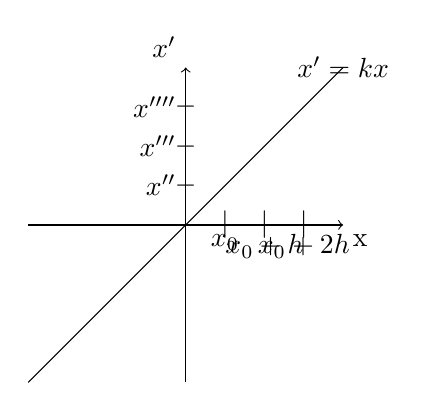
\begin{tikzpicture}[scale=1] %[x={10.0pt},y={10.0pt}]
	\pgfmathsetmacro\MAX{2}
	\draw[->] (-\MAX,0) -- (\MAX,0) node[anchor=north west] {x};
	\draw[->] (0,-\MAX) -- (0,\MAX) node[anchor=south east] {$ x'$};
	\draw[domain=-2:2,smooth,variable=\x] plot ({\x},{\x}) node {$ x'=kx$};
	\draw node at (0.5,0) {$|$};
	\draw node at (1,0) {$|$};
	\draw node at (1.5,0) {$|$};
	\draw node at (0,0.5) {$-$};
	\draw node at (0,1) {$-$};
	\draw node at (0,1.5) {$-$};
	\draw node[anchor=north] at (0.5,0) {$x_0$};
	\draw node[anchor=north] at (1,0) {$x_0+h$};
	\draw node[anchor=north] at (1.5,0) {$x_0+2h$};
	\draw node[anchor=east] at (0,0.5) {$ x'' $};
	\draw node[anchor=east] at (0,1) {$ x''' $};
	\draw node[anchor=east] at (0,1.5) {$ x''''$};
	
	\end{tikzpicture}% pic 1
	\qquad % <----------------- SPACE BETWEEN PICTURES
	\begin{tikzpicture}[scale=1] %[x={10.0pt},y={10.0pt}]
	\pgfmathsetmacro\MAX{2}
	\draw[->] (-\MAX,0) -- (\MAX,0) node[anchor=north west] {t};
	\draw[->] (0,-\MAX) -- (0,\MAX) node[anchor=south east] {x};
	\end{tikzpicture}% pic 2
\end{center}

blablabla ....\\
.......\\
Limiti di questo modello:
\begin{itemize}
	\item la variabile $x$ dovrebbe variare in $\N$, poiché una popolazione ha un numero intero di elementi.
	\item In molte specie è verosimile che il numero di nati al tempo $t$ dipenda dalla popolazione presente ad un tempo precedente $x(t-T), T>0$
	\item Supporre che una popolazione abbia per sempre a disposizione risorse sufficienti può non essere realistico
	\item Questo modello va bene quando si considerano intervalli di tempo molto lunghi.
\end{itemize}
\chapter{Calcolo delle Variazioni}
\section{Preliminari}
Il calcolo delle variazioni si occupa dell'ottimizzazione di funzioni $ F : X \to \R $, dove $X$ è un insieme di funzioni.\\
In questo capitolo varranno considerati univocamente funzionali integrali del tipo
\[\begin{array}{rcl} F: X & \to & \R \\
x & \to & \int_{a}^b f(t,x(t), x'(t))\integrald{t}\end{array}\]
eventualmente soggetti a vincoli sui valori $x(a)$ e $x(b)$ o sul valore di un integrale del tipo $\int_a^b \varphi(x(t))\integrald{t}$.\\
Dove:
\[f: \intervalclose{a}{b}\times \R ^n\times \R ^n \to \R\]
\[X=\brackets{x\in \cntclass{1}(\intervalclose{a}{b}); \R ^n\text{ t.c.: }x(a)=x_a, x(b)=x_b },\text{ con }x_a,x_b\in \R ^n\]
\proposition
Sia $f\in \cntclass{1}(A\times \R ; \R )$ con $a\subseteq \R ^n$\\
Se $\begin{array}{ccc} F: \R \times \R \times A & \to & \R \\
x & \to & \int_{\alpha}^\beta f(x,t)\integrald{t}\end{array}$
Allora:
\[ F\in \cntclass{1}\]
\[ \partial_\alpha F(\alpha,\beta,x)=-f(x,\alpha)\]
\[ \partial_\beta F(\alpha,\beta,x)=f(x,\beta)\]
\[ \nabla_x F(\alpha,\beta,x)=\int_{\alpha}^{\beta}\nabla_xf(x,t)\integrald{t}\]
\definition ?????????????? R OPPURE RN\\
Sia $I\in \R $ un intervallo. Curva su $I$ $ \R \bydef$ una funzione $\gamma:I\subseteq \R ^n$ che sia continua.
\observation
$\gamma(I)$ si chiama supporto della curva,ed 1'e certamente connesso.(una funzione continua manda intervalli connessi in connessi)
\definition
Sia $\gamma : \intervalclose{a}{b} \to \R^n$ una curva, allora
\[
	\begin{gathered}
		\text{lunghezza della curva }\\
		\bydef\\
		l(\gamma)=\sup\brackets{\sum\limits_{i=1}^{N}\norm{\gamma(t_i)-\gamma(t_{i-1})}: N\in\mathbb{N}\,N>1,t_0=a,t_N=b,t_{i-1}<t_i, i=1,2,\ldots,N}
	\end{gathered}
\]
cioè prendo una curva e la approssimo con una spezzata, la più lunga di tutte le poligonali è la lunghezza della curva.\\
DISEGNO\\
DISEGNO\\
\definition
Una curva $\gamma : \intervalclose{a}{b} \to \R^n$ si dice rettificabile $\bydef f(\gamma)<+\infty$
\observation
\[\sum\limits_{i=1}^{N}\norm{\gamma(t_i)-\gamma(t_{i-1})} \]
per il teorema del valore medio differenziale(accrescimenti finiti)
\[\sum\limits_{i=1}^{N}\norm{ \gamma'(t_i)(t_i-t_{i-1})} =??\]
\[\int_{a}^{b}\norm{ \gamma'(t)} \integrald{t}\]
\proposition
Se $\gamma\in \cntclass{1}(\intervalclose{a}{b}; \R ^n)\implies l(\gamma)=\int_a^b\norm{\gamma'(t)}\integrald{t}$
\observation
Se $\gamma$ è la traiettoria di un punto materiale,allora $\norm{\gamma}$ è la norma della velocità istantanea, e quindi $l(\gamma)$ è lo spazio che si percorre, cioè l'integrale della velocità valutato tra $t??????t_i$ due istanti di tempo entro i quali si mantiene tale velocità.
\observation
Nel caso specifico sarà:
\[ X=\brackets{ x\in \cntclass{1}(\left[a,b\right]; \R 2): x(a)=A, x(b)=B } \]
\[\begin{array}{ccc} 
F: X & \to & \R \\
x & \to & \int_{a}^b \norm{x'(t)}\integrald{t}
\end{array}\]
\[\begin{array}{ccc} 
f: \left[a,b\right]\times \R ^2\times \R ^2 & \to & \R \\
(t,x, x') & \to &  \norm{x'(t)}
\end{array}\]
\newpage
\section{L'Equazione di Eulero}
LEMMA:::LEMMA FONDAMENTALE DEL CALCOLO DELLE VARIAZIONI\\
Sia $f\in \cntclass{0}(\left[0,1\right]; \R )$ t.c.: $\forall v\in \cntclass{0}(\left[0,1\right]; \R )$ con $v(0)=v(1)=0$ si abbia $\int_0^1 f(x)v(x)\integrald{x}=0$\\
Allora $f(x)\equiv 0\forall x\in\left[0,1\right]$ 
\begin{proof}
	\begin{center}
		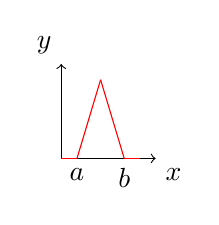
\begin{tikzpicture}[scale=1]
			\draw[->] (0,0) -- (1.2,0) node[anchor=north west] {$x$};
			\draw[->] (0,0) -- (0,1.2) node[anchor=south east] {$y$};
			\node[below] at (0.2,0) {$a$};
			\node[below] at (0.8,0) {$b$};
			\clip (0,0) rectangle (1,1);
			\draw[domain=0:0.2,smooth,red,variable=\x] plot ({\x},{0});
			\draw[domain=0.2:0.5,smooth,red,variable=\x] plot ({\x},{(1/0.3)*\x-(0.2/0.3)});
			\draw[domain=0.5:0.8,smooth,red,variable=\x] plot ({\x},{-(1/0.3)*\x+(0.8/0.3)});
			\draw[domain=0.8:1,smooth,red,variable=\x] plot ({\x},{0});
		\end{tikzpicture}
	\end{center}
	Per Assurdo, se $f\not\equiv 0$, allora $\exists\left[0,1\right]$ t.c. $f(x_0)\ne 0$.\\
	Osservo che se $x_0=0$ allora $\exists\overline{x}_0\in\left]0,1\right[$ t.c. $f(\overline{x}_0)\ne 0$.\\
	Osservo che se $x_0=1$ allora $\exists\overline{x}_0\in\left]0,1\right[$ t.c. $f(\overline{x}_0)\ne 0$\\
	Entrambe le osservazioni per la continuità di $f$, significa che se $x_0$ è un punto in cui la $f>0$ allora per la continuità della funzione anche li vicino si hanno valori maggiori di zero.\\
	Quindi si può pensare $x_0\in\left]0,1\right[$.\\
	Allora $\exists a,b\in\left]0,1\right[$ t.c. $x_0\in\left]a,b\right[ e \forall x\in\left]a,b\right[$ vale che $\abs{f(x)} \geq\abs{f(x_0)}$ sempre per la continuità di $f$.\\
	Pensiamo $f(x_0)>0$ in questo modo $\abs{f(x_0)}=f(x_0)$ e scegliamo la funzione $v(x)$ come disegnata: $v(x)=\left\{\begin{matrix}
	0&&x \leq x_0-\delta\\
	\frac{x}{\delta}-\frac{x_0-\delta}{\delta}&& x_0-\delta<x<x_0\\
	1&& x=x_0\\
	-\frac{x}{\delta}+\frac{x_0+\delta}{\delta}&&x_0<x<x_0+\delta\\
	0&&x \geq x_0+\delta
	\end{matrix}\right.$POSSIBILIPLAUSIBILIERRORI\\
	Se calcoliamo
	\[\int_0^1f(x)v(x)\integrald{x}=\int_a^bf(x)v(x)\integrald{x} \geq\frac{1}{2}f(x_0)\int_a^bv(x)\integrald{x}=\frac{1}{2}f(x_0)\frac{b-a}{2}>0\]
	Se avessi preso $f(x_0)<0$ prendo $v=-v$ e il resto segue...
\end{proof}
\observation
Questo lemma è concettualmente analogo al Teorema di Fermat nel capitolo delle derivate.
\corollary LEMMA CASO VETTORIALE.\\
Sia $f\in \cntclass{0}(\left[a,b\right]; \R ^n)$ tale che $\forall v\in \cntclass{0}(\left[a,b\right]; \R ^n)$ con $v(0)=v(1)=0$ si abbia $\int_0^1f(x)\bullet v(x)\integrald{x}=0$ allora $f(x)\equiv 0$ $\forall x\in \left[0,1\right]$.
\begin{proof}
	Per questa dimostrazione si osservano componente per componente.\\
	$\forall i=1,2,\ldots,n$ scelgo $v_j(x)=\left\{\begin{matrix}0&&j\ne i\\v_i(x)&&j=i \end{matrix}\right.$\\
	A questo punto applico il lemma fondamentale alla componente $i$-esima $f_i$ di $f$.
\end{proof}
\corollary
Sia $f\in \cntclass{0}(\left[a,b\right]; \R )$ e $k\in\mathbb{N}$ tale che $\forall v\in \cntclass{k}(\left[a,b\right]; \R ^n)$ con $v(0)=v(1)=0$ si abbia $\int_0^1f(x)v(x)\integrald{x}=0$ allora $f(x)\equiv 0$ $\forall x\in \left[0,1\right]$.
\begin{proof}
	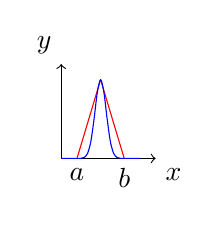
\begin{tikzpicture}[scale=1]
		\draw[->] (0,0) -- (1.2,0) node[anchor=north west] {$x$};
		\draw[->] (0,0) -- (0,1.2) node[anchor=south east] {$y$};
		\node[below] at (0.2,0) {$a$};
		\node[below] at (0.8,0) {$b$};
		\clip (0,0) rectangle (1,1);
		\draw[domain=0:0.2,smooth,red,variable=\x] plot ({\x},{0});
		\draw[domain=0.2:0.5,smooth,red,variable=\x] plot ({\x},{(1/0.3)*\x-(0.2/0.3)});
		\draw[domain=0.5:0.8,smooth,red,variable=\x] plot ({\x},{-(1/0.3)*\x+(0.8/0.3)});
		\draw[domain=0.8:1,smooth,red,variable=\x] plot ({\x},{0});
		\draw[domain=0:1,smooth,blue,variable=\x] plot ({\x},{ e^(-((\x-0.5)*10)^2) });
	\end{tikzpicture}
	\'E sempre lo stesso lemma con l'aggiunta che la funzione $v$ sia di classe $\cntclass{k}$.\\
	Se si chiama $u$ la funzione blu e $v$ la funzione rossa abbiamo:
	\[\int_0^1 f(x)u(x)\integrald{x}>0\]
	Se $v$ è un po più regolare , prendiamo $v=u^(k+1)(x)$. cioè se vogliamo $v\in \cntclass{k}$ prendiamo.....\\
	LA DINMOSTRAZIONE E A ME INCOMPRENSIBILE.
\end{proof}

\theorem EQUAZIONE DI EULERO.\\
Sia $f\in \cntclass{2}\left(\left[a,b\right]\times \R ^n\times \R ^n; \R \right)$ con $a,b\in \R $ e $a<b$.\\
Sia $X=\brackets{x\in \cntclass{2}\left(\left[a,b\right]; \R ^n\right): x(a)=A, x(b)=B}$ con $A,B\in \R ^n$.\\
Sia $\begin{array}{ccc} F: X & \to & \R \\
x & \to & \int_{a}^b f(t,x(t), x'(t))\integrald{t}\end{array}$.\\
Se la funzione $x_\ast\in X$ è t.c. $F(x_\ast)=\max\brackets{F(x):x\in X }$ [o min]\\
Allora $\partial_xf(t,x_\ast(t), x_\ast'(t))-\frac{d}{\integrald{t}}\partial_{ x'}f(t,x_\ast(t), x_\ast'(t))=0$.\\
Questa ultima equzione è l'equazione di Eulero-Lagrange del Funzionale $F$ o a volte detta variazione prima del funzionale $F$. è un sistema di $n$ equazioni differenziali ordinarie del secondo ordine nella funzione incognita $x_\ast$.
\begin{proof}
	 Sia $\varphi(h)=F(x_\ast+hv)$, dove $x_\ast\in X$ e $x_\ast+hv\in X$, con $h$ piccolo.\\
	 L'equazione di Eulero-Lagrange in apparenza complicata è analoga ad un equazione di analisi1 del tipo $f'=0$ oppure in analisi due a $\nabla f=0$. solo che ora sono cavoli amari.\\
	 Come si sceglie la variazione $v$ in modo che $x_\ast+hv\in X$, con $h$ piccolo.\\
	 $X$ è l'insieme delle funzioni di $\cntclass{2}$, si sa che $x_\ast\in \cntclass{2}$, una scelta opportuna di $v$ è $v\in \cntclass{2}(\left]a,b\right[; \R ^n)$.\\
	 Inotre deve essere che $ x_\ast(a)+hv(a)=A$ e  $x_\ast(b)+hv(b)=B$ per restare dentro l'insieme $X$.
	 Quindi $v(a)=v(b)=0$.
	 $h$ è uno scalare e per ipotesi si sa che $F(x_\ast)$ è punto di massimo, quindi si conclude che $h=0$ è punto di massimo per la funzione $\varphi$.\\
	 ........ 
\end{proof}
e qui finiscono gli appunti almeno per conto mio.



% a me questo tentativo di tema esame che avevo fatto fa un po pena
% poverino è li solo soletto ed incompleto ... io lo toglierei
\chapter{Temi Esame}
\section{T.E. 2012/2013 scritto n.1}
\begin{exercise}
	Sia $f: \R^2 \to \R$ data da $f(x, y)=e^{-\abs{4\cdot arctan(x\cdot y^2)}}$
	\begin{description}
		\item[A] Nessuna delle altre affermazioni è esatta
		\item[B] $f$ ammette almeno un punto di minimo assoluto
		\item[C] $\inf_R^2f = 0$
		\item[D] $f$ ha infiniti punti di massimo
	\end{description}
	L'esponensiale è una funzione monotona crescente quindi la ricerca di massimi a minimi si sposta alla ricerca dei massimi e minimi dell'esponente.\\
	L'esponente assume sempre valori negativi. Inotre risulta essere una quantità limitata tra $[0;4\frac{\pi}{0}[$, quindi $\sup_R^2f=e^0=1$ e $\inf_R^2f=e^{-2\pi}$\\
	Sono quindi punti di massimo tutti i punti che rendono nullo l'esponente: $arctan(xy^2)=0 \implies x=0,\forall y or y=0,\forall x$ che sono i due assi. Essendo questi punti del dominio allora si può dire $\sup_R^2f=\max_R^2f=0$\\
	I punti di minimo si hanno per $\abs{arctan(xy^2)}=\frac{\pi}{2}$ quindi per $x \to \pm\infty$ or $y \to \pm\infty$ essendo questi valori al limite il valore $e^{-2\pi}$ è $inf$ per $f$\\
	La risposta vera è quindi la D.\\
\end{exercise}
\begin{exercise}
	Sia $(X,d)$ uno spazio metrico e siano $A, B$ sottoinsiemi di $X$. Quale/i delle seguenti affermazioni è/sono certamente vera/e?
	\begin{description}
		\item[1] $A\subseteq B \implies\partial A\subseteq \partial B$
		\item[2] $A\subseteq B \implies\overline{A}\subseteq\overline{B}$
	\end{description}
	\begin{description}
		\item[A] Entrambe
		\item[B] Solo la seconda
		\item[C] Nessuna delle affermazioni è esatta
		\item[D] Solo la prima
	\end{description}
	La prima affermazione è certamente falsa poiché se scelto come spazio metrico $R^2$ con distanza quella eclidea. Scelgo $A=B((0,0),2), A=B((0,0),1)$ allora si ha che $\partial A = \{(x,y)\in \R^2:d((x,y),(0,0))=2\}$ e $\partial B = \{(x,y)\in \R^2:d((x,y),(0,0))=1\}$ e questi due insiemi sono disgiunti.\\
	la seconda è vera ma devo pensarci un po...\\
\end{exercise}



\renewcommand{\thesection}{\Alph{section}} % Using letters for appendix sections
\begin{appendices}
\section{Forme Quadratiche}\label{sect:for_quadr}
In questa sezione saranno riportati solo i risultati più importanti sulle forme quadratiche, quelli necessari alla ricerca di punti estremanti di funzioni a più variabili. Nel dettaglio, si vedrà come stabilire il segno di una forma quadratica.

Per un'esposizione dettagliata e completa si rimanda ad un libro di Algebra Lineare.

\begin{definition}[Forma Quadratica]
	\label{def:form_quadr}
	\textbf{Forma Quadratica} su $\R^n$ è una funzione del tipo
	\[\funcdef{q}{\R^n}{\R}{x}{x^T Q \: x}\]
	Dove:
	\begin{itemize}[noitemsep]
		\item $x^T \in \mat(1 \times n)$ è vettore riga trasposto del vettore colonna $x \in \mat(n \times 1)$
		\item $Q \in \mat(n \times n)$
	\end{itemize}

	\noindent Inoltre, per come è definito il prodotto righe per colonne, la $q$ può essere riscritta come
	\[q(x) = \sum\limits_{i, j = 1}^{n} q_{ij}\:x_i\:x_j\]
	con $q_{ij}$ elemento nella riga $i$ e nella colonna $j$ della matrice $Q$.
\end{definition}
\begin{exercise}
	Dimostrare che $q$ è una forma quadratica su $\R^n$ se e solo se $q(x)$ è un polinomio omogeneo di grado $2$ in funzione di $x$
	\begin{solution}
		Direttamente dalla \fullref{def:form_quadr} in forma di sommatoria, si ha un polinomio di grado $2$ nelle variabili $x_1, \;\dotsc\;, x_n$
		\[\sum\limits_{i, j = 1}^{n} q_{ij}\:x_i\:x_j \quad = \quad q_{11}x_1^2 + q_{12}x_1x_2 + \cdots q_{nn}x_n^2\]
	\end{solution}
\end{exercise}
\begin{proposition}
	\label{prop:proprieta_form_quadr}
	Sia $q$ forma quadratica su $\R^n$, allora:
	\begin{enumerate}
		\item \label{itm:form_quadr_lambda} $\forall \lambda \in \R,\; \forall x \in \R^n$ vale $q(\lambda x) = \lambda^2 q(x)$
		\item $q(0) = 0$
		\item $q$ è \textbf{limitata} $\implies$ $q$ è \textbf{identicamente nulla} (cioè $q(x) = 0 \; \forall x \in \R^n$)
	\end{enumerate}
	\begin{proof}\hfill
		\begin{enumerate}
			\item $q(\lambda x) = (\lambda x)^T Q \: (\lambda x) = \lambda^2 x^T Q \: x = \lambda^2 q(x)$
			\item $q(0) = q(0 \cdot 0)$, prendendo poi dal punto precedente, $q(0 \cdot 0) = 0^2 \; q(0) = 0$
			\item Si dimostra la contronominale (cioè la negazione dell'implicazione inversa)\\
				$q$ non identicamente nulla $\implies \exists x \in \R^n:\; q(x) \neq 0 \implies \forall \lambda \in \R \quad q(\lambda x) = \lambda^2 q(x) \implies q$ non limitata
		\end{enumerate}
	\end{proof}
\end{proposition}
\begin{proposition}
	\label{prop:form_quadr_M}
	Data $q$ forma quadratica su $\R^n$, allora esiste una costante $M$ tale che
	\[\forall x \in \R^n \qquad \abs{q(x)} \leq M \norm{x}^2\]
	\begin{proof}
		Grazie al punto \ref{itm:form_quadr_lambda} della \fullref{prop:proprieta_form_quadr}, si sa che
		\begin{equation}
			\label{eq:form_quadr_M}
			\abs{q(x)} = \abs{q \left( \norm{x} \frac{x}{\norm{x}} \right)} = \norm{x}^2 \; \abs{q \left( \frac{x}{\norm{x}} \right)}
		\end{equation}
		$\frac{x}{\norm{x}}$ è il \textbf{Versore} di $x$ (il vettore direzione con norma $= 1$) quindi, $\forall x \in \R^n$, si sta lavorando soltanto sui punti appartenenti a $\partial B(0,1)$: la frontiera della sfera di raggio $1$.\\
		Sia dunque $M = \max\limits_{\partial B(0,1)} q(x)$. $\partial B(0,1)$ è un compatto, essendo insieme chiuso e limitato in $\R^n$ (vedasi \fullref{prop:compat_chius_lim}). Grazie alla regolarità di $q$ ed alla compattezza di $\partial B(0,1)$, si può applicare l'\fullref{ex:weier_analisi_1} ed avere la certezza dell'esistenza di un $M$ finito.\\
		Verificata l'esistenza di $M$, massimo sulla $\partial B(0,1)$, è sicuramente possibile minorare l'ultimo termine di \cref{eq:form_quadr_M} ed ottenere la tesi
		\[\abs{q(x)} = \norm{x}^2 \; \abs{q \left( \frac{x}{\norm{x}} \right)} \leq M \norm{x}^2\]
	\end{proof}
\end{proposition}
\begin{corollary}
	Data $q$ forma quadratica su $\R^n$, allora:
	\[\forall \alpha \in \intervalclop{0}{2} \qquad q(x) = o(\norm{x}^\alpha) \text{ per } x \to 0\]
	\begin{proof}
		Immediata dalla \fullref{prop:form_quadr_M} perché si ha già dimostrato che esista un certo $M$ per cui $q(x) \leq M \norm{x}^2$. Basta applicare la \fullref{def:o_piccolo} a $x \to 0$ per arrivare alla tesi.
	\end{proof}
\end{corollary}
\begin{proposition}
	Data $q$ forma quadratica su $\R^n$, allora:
	\[\abs{q(x)} = o(\norm{x}^2) \text{ per } x \to 0 \quad \iff \quad q(x) = 0 \qquad \forall x \in \R^n\]
	\begin{proof}~
		\begin{itemize}
			\item[$\implies$] Sia $x \in \R^n$ con $\norm{x} = 1$ (quindi $x$ \textbf{Versore}). Si applica la \fullref{def:o_piccolo}
				\begin{align*}
					0 &= \lim\limits_{t \to 0} \frac{\norm{q(tx)}}{\norm{tx}^2}\\
					\shortintertext{Essendo $q(tx) \in \R$, la norma corrisponde al valore assoluto}
					&= \lim\limits_{t \to 0} \frac{\abs{q(tx)}}{\norm{tx}^2}
					\shortintertext{Utilizzando il punto \ref{itm:form_quadr_lambda} della \fullref{prop:proprieta_form_quadr} e la proprietà \ref{itm:norm_lambda} da \fullref{def:norma}}
					&= \lim\limits_{t \to 0} \frac{\abs{t^2 q(x)}}{\abs{t}^2 \norm{x}^2}
					 = \lim\limits_{t \to 0} \frac{\abs{t^2} \abs{q(x)}}{\abs{t}^2 \norm{x}^2}
					 = \frac{\abs{q(x)}}{\norm{x}^2} \; \lim\limits_{t \to 0} \frac{t^2}{t^2}
					 = \frac{\abs{q(x)}}{\norm{x}^2}
					\shortintertext{Essendo per ipotesi $\norm{x} = 1$}
					&= \abs{q(x)}
				\end{align*}
				Ma, avendo un valore assoluto $= 0$, è sicuramente vero che
				\[0 = \abs{q(x)} = q(x)\]
				Da cui la tesi
			\item[$\impliedby$] Immediatamente applicando la \fullref{def:o_piccolo}, in quanto si avrebbe
				\[\lim\limits_{x \to x_0} \frac{\norm{q(x)}}{\norm{x}^2} = \lim\limits_{x \to x_0} \frac{0}{\norm{x}^2} = 0\]
		\end{itemize}
	\end{proof}
\end{proposition}
\begin{definition}
	\label{def:def_semdef_pos_neg}
	Data $q$ forma quadratica su $\R^n$ individuata dalla matrice $Q$, allora $q$ è:
	\begin{itemize}
		\item \makebox[11em][l]{\textbf{Definita Positiva}} \makebox[15em][l]{$\quad \bydef \quad \forall x \in \R, x \neq 0 \quad q(x) > 0$} $\bydef \quad Q > 0$
		\item \makebox[11em][l]{\textbf{Semidefinita Positiva}} \makebox[15em][l]{$\quad \bydef \quad \forall x \in \R \quad q(x) \geq 0$} $\bydef \quad Q \geq 0$
		\item \makebox[11em][l]{\textbf{Definita Negativa}} \makebox[15em][l]{$\quad \bydef \quad \forall x \in \R, x \neq 0 \quad q(x) < 0$} $\bydef \quad Q < 0$
		\item \makebox[11em][l]{\textbf{Semidefinita Negativa}} \makebox[15em][l]{$\quad \bydef \quad \forall x \in \R \quad q(x) \leq 0$} $\bydef \quad Q \leq 0$
	\end{itemize}
	\begin{note}
		La definizione più a destra, quella che utilizza i segni $\gtrless$, è sconsigliabile in quanto fuorviante: non esiste relazione d'ordine tra matrici.
	\end{note}
\end{definition}
\begin{exercise}
	Esibire un esempio di forma quadratica su $\R^2$ per ognuno dei tipi sopra definiti.\\
	Esibire un esempio di forma quadratica su $\R^2$ non definita.
	\begin{solution}~
		\begin{enumerate}
			\item Semidefinita positiva
				\[ Q =
					\begin{bmatrix}
						2 & 0\\
						0 & 3
					\end{bmatrix}
					\qquad
					q(x,y) = 2x^2 + 3y^2
				\]
			\item Definita positiva
				\[ Q =
					\begin{bmatrix}
						1 & -1\\
						-1 & 3
					\end{bmatrix}
					\qquad
					q(x,y) = x^2 - 2xy + 3y^2
				\]
				\[\left( \frac{x}{y} \right)^2 - 2\left( \frac{x}{y} \right) + 3 > 0\]
			\item Semidefinita negativa
				\[ Q =
					\begin{bmatrix}
						-3 & 0\\
						0 & 0
					\end{bmatrix}
					\qquad
					q(x,y) = -3x^2
				\]
			\item Definita negativa
				\[ Q =
					\begin{bmatrix}
						-1 & \sqrt{2}\\
						\sqrt{2} & -2
					\end{bmatrix}
					\qquad
					q(x,y) = -x^2 + 2\sqrt{2}xy - 2y^2
				\]
			\item Nè definita nè semidefinita
				\[ Q =
					\begin{bmatrix}
						1 & 0\\
						0 & -1
					\end{bmatrix}
					\qquad
					q(x,y) = x^2 - y^2
				\]
				\[q(1,0) = 1 \qquad\qquad q(0,1) = -1\]
		\end{enumerate}
	\end{solution}
\end{exercise}
\begin{exercise}
	In $\mat (n \times n)$, sia definita la relazione d'ordine $>$ da
	\[M_1 > M_2 \quad \bydef \quad M_1 - M_2 > 0\]
	La relazione $>$ è una relazione di ordine totale?
	% TODO solution
\end{exercise}
\begin{proposition}
	\label{prop:form_quadr_def_pos_q_geq_m}
	Data $q$ forma quadratica su $\R^n$, allora:
	\[
		q \text{ \textbf{Definita Positiva}} \quad \iff \quad \exists m > 0:\; \forall x \in \R^n \quad q(x) \geq m \norm{x}^2
	\]

	\begin{proof}~
		\begin{itemize}
			\item[$\implies$] Si procede con un procedimento analogo a quello della \fullref{prop:form_quadr_M}.\\
				Grazie al punto \ref{itm:form_quadr_lambda} della \fullref{prop:proprieta_form_quadr}, si sa che
				\begin{equation}
					\label{eq:form_quadr_def_pos}
					q(x) = q \left( \norm{x} \frac{x}{\norm{x}} \right) = \norm{x}^2 \; q \left( \frac{x}{\norm{x}} \right)
				\end{equation}
				Per gli stessi motivi dell'altra dimostrazione, si può porre $m = \min\limits_{\partial B(0,1)} q(x)$ ed avere la certezza che esista finito. Inoltre, sicuramente $m \geq 0$ perché $q$ è definita positiva per ipotesi.\\
				È dunque sicuramente possibile maggiorare l'ultimo termine di \cref{eq:form_quadr_def_pos} ed ottenere la tesi
				\[q(x) = \norm{x}^2 \; q \left( \frac{x}{\norm{x}} \right) \geq m \norm{x}^2\]
			\item[$\impliedby$] Immediata.
		\end{itemize}
	\end{proof}
\end{proposition}
\begin{corollary}
	\label{coro:form_quadr_def_neg_q_leq_-m}
	Data $q$ forma quadratica su $\R^n$, allora:
	\[
		q \text{ \textbf{Definita Negativa}} \quad \iff \quad \exists m > 0:\; \forall x \in \R^n \quad q(x) \leq -m \norm{x}^2
	\]
	\begin{proof}
		Analoga alla precedente
	\end{proof}
\end{corollary}

\vspace*{\baselineskip}
Grazie alle seguenti proposizioni viene fornito metodo più rapido per verificare la definizione/semidefinizione delle forme quadratiche.
\begin{proposition}[Ortogonalizzazione di Gram-Schmidt]
	\label{prop:gram_schm}
	Data $q$ forma quadratica \textbf{definita positiva} o \textbf{negativa} su $\R^n$ con matrice \textbf{simmetrica} $Q$.\\
	Esiste un sistema di coordinate in cui la matrice $\tilde{Q}$ di $q$ è diagonale ed ha come coefficienti
	\[Q_1 \qquad \frac{\det Q_2}{\det Q_1} \qquad \frac{\det Q_3}{\det Q_2} \qquad \dotsc \qquad \frac{\det Q_n}{\det Q_{n-1}}\]
	dove $Q_i$ è la matrice costituita dalle prime $i$ righe ed $i$ colonne di $Q$ ("come negli orlati").
	\begin{note}
		Non è necessario conoscere il sistema di coordinate in cui è valida l'uguaglianza, ai fini dello studio di una Forma Quadratica è sufficiente sapere che esso esiste e che l'uguaglianza è valida.
	\end{note}
	\begin{center}
		\begin{tikzpicture} [
			nodes = {anchor=center}
		]
			\matrix (Q) [
				matrix of math nodes,
				left delimiter = {[}, right delimiter = {]},
				nodes in empty cells,
				minimum width = 2.5em, minimum height = 2.5em
			]{
			Q_1 &	&	&	\\
				& Q_2 &	&	\\
				&	& \ddots &\\
				&	&	& Q_n\\
			};

			\draw[dashed] (Q-1-1.south west) -- (Q-1-1.south east);
			\draw[dashed] (Q-1-1.south east) -- (Q-1-1.north east);
			\draw[dashed] (Q-2-1.south west) -- (Q-2-2.south east);
			\draw[dashed] (Q-2-2.south east) -- (Q-1-2.north east);
			\draw[dashed] (Q-3-1.south west) -- (Q-3-3.south east);
			\draw[dashed] (Q-3-3.south east) -- (Q-1-3.north east);

			\node at ([xshift=2.5em] Q.east) {$=$};

			\matrix at ([xshift=12em] Q.east) [
				matrix of math nodes,
				left delimiter = {[}, right delimiter = {]},
				nodes in empty cells,
				minimum width = 2.5em, minimum height = 2.5em
			]{
			\det Q_1 &	&	&	\\
				& \frac{\det Q_2}{\det Q_1} &	&	\\
				&	& \ddots &\\
				&	&	& \frac{\det Q_n}{\det Q_{n-1}}\\
			};
		\end{tikzpicture}
	\end{center}
	\begin{proof}
		Omessa.
	\end{proof}
	\begin{note}
		Questa enunciazione dell'ortogonalizzazione di Gram-Schmidt sembra privilegiare le sottomatrici costituite dalle prime righe e dalle prime colonne. È però possibile enunciare una versione di questa proposizione in cui tutte le sottomatrici quadrate costruite attorno alla diagonale hanno gli stessi \textit{privilegi}.
	\end{note}
\end{proposition}
\begin{observation}
	Nella \fullref{prop:gram_schm}, l'ipotesi che $q$ sia definita assicura che le diverse $Q_i$ per $i = 1,\:\dotsc\:,n$ siano non nulle.\\
	Nel caso in cui $q$ non fosse definita sarebbe ancora possibile diagonalizzare $q$ ottenendo una matrice diagonale con gli "ultimi" elementi della diagonale nulli.
\end{observation}
\begin{corollary}
	\label{coro:def_pos_neg_segni_Q}
	Data $q$ forma quadratica su $\R^n$ con matrice \textbf{simmetrica} $Q$.
	\begin{align*}
		Q \text{ Definita Positiva }
		\quad &\iff \quad
		\begin{cases}
			q_1 > 0\\
			\det Q_2 > 0\\
			\det Q_3 > 0\\
			\vdots\\
			\det Q_n > 0
		\end{cases}\\
		Q \text{ Definita Negativa }
		\quad &\iff \quad
		\begin{cases}
			-q_1 > 0\\
			\det Q_2 > 0\\
			-\det Q_3 > 0\\
			\vdots\\
			(-1)^n \; \det Q_n > 0
		\end{cases}
	\end{align*}
	dove $Q_i$ è la matrice costituita dalle prime $i$ righe ed $i$ colonne di $Q$ ("come negli orlati").

	Cioè se tutte le sottomatrici hanno determinante positivo, allora la $Q$ è Definita Positiva. Se invece i determinanti hanno segni alternati (partendo da una negativa), allora è Definita Negativa.
	\begin{proof}
		Omessa.
	\end{proof}
\end{corollary}
\begin{exercise}
	Dimostrare il \fullref{coro:def_pos_neg_segni_Q}. Suggerimento: applicare la \fullref{prop:gram_schm}.
	% TODO solution
\end{exercise}
\begin{exercise}
	Enunciare il \fullref{coro:def_pos_neg_segni_Q} nel caso $n = 2$ e verificarlo con i metodi dell'algebra elementare.\\
	Suggerimento: utilizzare la regola per determinare il segno di un polinomio di secondo grado.
	% TODO solution
\end{exercise}
\end{appendices}


\backmatter
\phantomsection
\cleardoublepage
\addcontentsline{toc}{chapter}{Indice Analitico}
\printindex

\end{document}